% to compile in windows:
% lualatex main.tex
%
% to compile bibtex
% bibtex main
%
% then refresh the pdf view to see changes if not reflected automatically
\documentclass[a4paper, 12pt, oneside]{book}
\usepackage[left=1.25in,top=1in,right=1in,bottom=1in]{geometry}
\usepackage[utf8]{inputenc}
\usepackage{booktabs}
\usepackage{float}
\usepackage{tabularx}
\usepackage{algorithm}
\usepackage{algpseudocode}
\usepackage{multirow}
\usepackage[framemethod=TikZ]{mdframed}
\usepackage{amsmath, amssymb, amsthm}
\usepackage{mdframed}
\usepackage{arabluatex}
\usepackage{tikz}
\usetikzlibrary{shapes,backgrounds,automata,chains,arrows,positioning,calc,patterns}
\usetikzlibrary{decorations.markings,arrows}
\usepackage{pgfplots}
\usepackage{pifont}
\usepackage{parnotes}
\usepackage{newpxmath} % math font is Palatino compatible
% \usepackage[nomath]{fontspec}
% \usepackage{amsmath}
\usepackage{subcaption}
\usepackage{pdflscape}
\usepackage{setspace}
\usepackage[explicit,compact]{titlesec}
\usepackage[hidelinks]{hyperref}
\usepackage{apacite} % load this after hyperref
\usepackage{listings}
\usepackage{xcolor} % For syntax highlighting colors
\usepackage{fancyvrb}
\usepackage{fontspec}
\usepackage{polyglossia}
\setmainlanguage{english}
\setotherlanguage{arabic}

\usepackage{newfloat}
\DeclareFloatingEnvironment[
    fileext=loi,
    listname={List of Listings},
    name=Listing,
    placement=tbhp,
]{listing2}

\mdfdefinestyle{mystyle}{
    linewidth=1pt,
    linecolor=black,
    topline=true,
    bottomline=true,
    leftline=true,
    rightline=true,
    innertopmargin=10pt,
    innerbottommargin=15pt,
    innerrightmargin=10pt,
    innerleftmargin=10pt,
    roundcorner=5pt
}

\newenvironment{bottomtitledframe}[1]{%
    \par\vspace{0.5cm}
    \begin{mdframed}[style=mystyle]
    \gdef\frameparamtitle{#1}% Store the parameter globally
}{%
    \end{mdframed}
    \par\vspace{-1.05cm}
    \centering\colorbox{white}{\textbf{\frameparamtitle}}% Use the stored parameter
    \par\vspace{0.5cm}
}

% arabluatex
\SetArbDflt*
\newarbmark{als}{^^^^fd47}{} % alayhis salam


% Basic configuration
\lstset{
    frame=single,
    breaklines=true,
    postbreak=\raisebox{0ex}[0ex][0ex]{\ensuremath{\hookrightarrow\space}},
    basicstyle=\ttfamily\small\singlespacing,
    keywordstyle=\color{blue}\bfseries,
    commentstyle=\color{green!60!black}\itshape,
    stringstyle=\color{red},
    numbers=left,
    numberstyle=\tiny\color{gray},
    numbersep=10pt,
    tabsize=4,
    showspaces=false,
    showstringspaces=false
}

\lstdefinelanguage{Julia}{
  keywords={
    abstract, baremodule, begin, bitstype, break, catch, ccall,
    const, continue, do, else, elseif, end, export, finally, for,
    function, global, if, immutable, import, importall, in,
    let, local, macro, module, quote, return, struct, try, type,
    typealias, using, while
  },
  sensitive=true,
  comment=[l]{\#},
  morecomment=[n]{\#=}{=\#},
  string=[b]",
  morestring=[b]',
  morestring=[b]"""
}

\setmainfont{TeX Gyre Pagella} 
\newfontfamily\arabicfont{Amiri}[Script=Arabic,RawFeature={+ss05}]
% remove this if you want to print it as paperback
\setlength\oddsidemargin{\dimexpr(\paperwidth-\textwidth)/2 - 1in\relax}
\setlength\evensidemargin{\oddsidemargin}

% arabluatex options
\SetTranslitConvention{arabica}
% \txarb{\fontspec{Scheherazade New} ﵇} - peace be upon him
% \txarb{\fontspec{Scheherazade New} ﵈} - peace be upon them (masculine)
% \txarb{\fontspec{Scheherazade New} ﵉} - peace be upon them (both)
% \txarb{\fontspec{Scheherazade New} ﵍} - peace be upon her
% \txarb{\fontspec{Scheherazade New} ﷺ} - sallalahu alayhi wa sallam
% \txarb{\fontspec{Scheherazade New} ﷾} - subhana wa ta'ala
% \txarb{\fontspec{Scheherazade New} ﷿} - azza wa jall


% mdframed options
% \definecolor{amethyst}{rgb}{0.6, 0.4, 0.8}
% \mdfdefinestyle{MyFrame}{%
%     linecolor=amethyst,
%     outerlinewidth=0.3pt,
%     roundcorner=3pt}
\newcounter{ortho}[section]\setcounter{ortho}{0}
\renewcommand{\theortho}{\arabic{section}.\arabic{ortho}}
\newenvironment{ortho}[2][]{%
\refstepcounter{ortho}%
\ifstrempty{#1}%
{\mdfsetup{%
frametitle={%
\tikz[baseline=(current bounding box.east),outer sep=0pt]
\node[anchor=east,rectangle,fill=orange!50]
{\strut Orthography~\theortho};}}
}%
{\mdfsetup{%
frametitle={%
\tikz[baseline=(current bounding box.east),outer sep=0pt]
\node[anchor=east,rectangle,fill=orange!50]
{\strut Orthography~\theortho:~#1};}}%
}%
\mdfsetup{innertopmargin=10pt,linecolor=orange!50,%
linewidth=1.5pt,topline=true,roundcorner=3pt,%
frametitleaboveskip=\dimexpr-\ht\strutbox\relax
}
\begin{mdframed}[]\relax%
\label{#2}}{\end{mdframed}}

\newcommand{\CI}{\mathrel{\perp\mspace{-10mu}\perp}}
\newcommand{\nCI}{\centernot{\CI}}
\newcommand{\ein}{\varepsilon_{\mathrm{in}}}
\newcommand{\eout}{\varepsilon_{\mathrm{out}}}
\newcommand{\Var}{\operatorname{Var}}
\newcommand{\ev}{\operatorname{E}}
\newcommand{\var}{\operatorname{Var}}
\newcommand{\p}{\mathbb{P}}
\newcommand{\af}{\varrho}
\newcommand{\I}{\mathbb{I}}
\newcommand{\D}{\operatorname{d}}
\newcommand{\dkl}{\mathbb{D}_{\mathrm{KL}}}
\newcommand{\f}{\mathbb{F}}
\newcommand{\set}{\overset{\text{set}}{=}}
\newcommand{\tr}{\mathrm{tr}}
\newcommand\numberthis{\addtocounter{equation}{1}\tag{\theequation}}
\newcommand{\g}{\mathbb{G}}
\newcommand{\idxa}{\textrm{\ding{70}}}
\newcommand{\idxb}{\textrm{\ding{72}}}
\newcommand{\idxc}{\textrm{\ding{86}}}
\newcommand{\post}{\textrm{\ding{71}}}
\newcommand{\F}{\mathtt{f}}
\newtheorem*{remark}{Remark}
\newtheorem{thm}{Theorem}[section]
\newtheorem{prop}{Proposition}[section]
\newtheorem{lem}{Lemma}[section]
\newtheorem{cor}{Corollary}[section]
\theoremstyle{definition}
\newtheorem{exmpx}{Example}[section]
\newtheorem{defnx}{Definition}[section]
\newenvironment{defn}
  {\pushQED{\qed}\renewcommand{\qedsymbol}{$\multimap$}\defnx}
  {\popQED\enddefnx}
\newenvironment{exmp}
  {\pushQED{\qed}\renewcommand{\qedsymbol}{$\multimapdot$}\exmpx}
  {\popQED\endexmpx}
  \newenvironment{warning}
  {\par\begin{mdframed}[linewidth=2pt,linecolor=gray]%
    \begin{list}{}{\leftmargin=.5cm
                   \labelwidth=\leftmargin}\item[\Large\ding{43}]}
  {\end{list}\end{mdframed}\par}

% for full expanding width table
\newcolumntype{Y}{>{\centering\arraybackslash}X}
\newcolumntype{s}{>{\hsize=.6\textwidth}c}

\def\title{\Large\bf Text Analytics of the Qur'\=an}
\def\author{Al-Ahmadgaid Bahauddin Asaad}
\def\program{\bf Master of Arts in Islamic Studies}
\def\ddate{June 2025}

\titleformat{\chapter}[block]
    {\vspace{-3cm}\bfseries\Large\centering}{\chaptertitlename}{0.5ex}{\;\bfseries\Large\thechapter\\#1}

\titleformat{name=\chapter,numberless}[block]
    {\vspace{-3cm}\bfseries\Large\centering}{#1}{0.5ex}{}

\titleformat{\section}[block]
    {\bfseries\normalsize}{\thesection}{0.5ex}{\;#1}

\titleformat{\subsection}[block]
    {\bfseries\normalsize}{\thesubsection}{0.5ex}{\;#1}

\begin{document} 
\begin{center}
\vspace{-2cm}\title
\end{center}
\addcontentsline{toc}{chapter}{Title Page}
\thispagestyle{empty}
{\baselineskip=1.0\baselineskip
\begin{center}
\vspace{2cm}
by\\
\vspace{3cm}
{\bfseries\author}\\
\vspace{3cm}
{
Submitted to the \textit{Institute of Islamic Studies}\\[0.2cm]
in partial fulfillment of the requirements for the degree of\\[.2cm]}
{\program}\\
\vspace{2.8cm}

\includegraphics[scale=0.08]{uplogo}\\[0.2cm]
{\large \textsc{University of the Philippines}}\\[0.2cm]
Diliman, Quezon City\\
\vspace{3.4cm}
{\ddate }
\end{center}

}
\doublespacing
% \chapter*{Dedication}
\addcontentsline{toc}{chapter}{Dedication}
\begin{center}
    \txarb{إلى الرجل المعروف لدى البعض كمخطط ومتحدث عام، ولكنه معروف لدى الكثيرين كمعلم، ومصمم، ونجار، وسائق دراجة ثلاثية، وصياد سمك، وبشكل خاص أب متواضع، أبانا العزيز، غرواس س. أسعد. نسأل الله أن يمنحك أعلى درجات الجنة، وأن يجمعنا جميعاً هناك. أشتاق إليك كثيراً، شكراً لك على كل شيء.}\\

    \textit{To the man known to some as a planner and a public speaker, but known to many as a teacher, designer, carpenter, tricycle driver, fisherman, and most especially a humble father, our dear papa, Garwas S. Asaad. May Allah \txarb{\fontspec{Scheherazade New} ﷿} bless you with the highest of} \arb{jannaT} \textit{, and may He unite us all there together. I miss you so much pa, magsukul ma kamemon.}\\
    \begin{minipage}{.6\linewidth}
        \centering
        \vspace{4cm}
        \arb[fullvoc]{'afalA yatadabbarUna 'l-qur'Ana walawkAna min `indi.gayri 'l-lahi lawajadUA" fIhi "axtilAfaN ka_tIraN}\\
        \textit{Will they not think about this Qur'an? If it had been from anyone other than God, they would have found much inconsistency in it.}\\
        {\sc Qur'an 4:82}\\[2cm]
        \arb[fullvoc]{wa`ibAdu 'l-ra.hmAni 'lla_dIna yam^sUna `alaY" 'l-'ar.di hawnaN wa-'i_dA xA.tabahumu\\
        'l-j---------------------Ahi---------------------lUna 
        q---------------------Al---------------------UA" sa---------------------lAm---------------------aN}\\
        \textit{The servants of the Lord of Mercy are those who walk humbly on the earth, and who, when aggressive people address them, reply, with words of Peace.}\\
        {\sc Qur'an 25:63}\\[1cm]
    \end{minipage}
\end{center}
% \chapter*{Acknowledgement}
\addcontentsline{toc}{chapter}{Acknowledgement}
{\centering

\includegraphics[scale = 1]{img/bismillah.jpg}\\[-.3cm]
(In the name of Allah, the Entirely Merciful, the Especially Merciful)\\[3cm]
}
\textit{The author would like to acknowledge his thesis adviser, Prof. Julkipli M. Wadi, for his patience and guidance; his thesis panels, Dr. Joselito C. Magadia (UPD School of Statistics), for his valuable insights on the theory, algorithm, and modeling aspect of the paper. Lastly, the author would like to acknowledge his family, friends, co-workers, and his chuchay for their moral support.}\\[2cm]
\begin{center}
    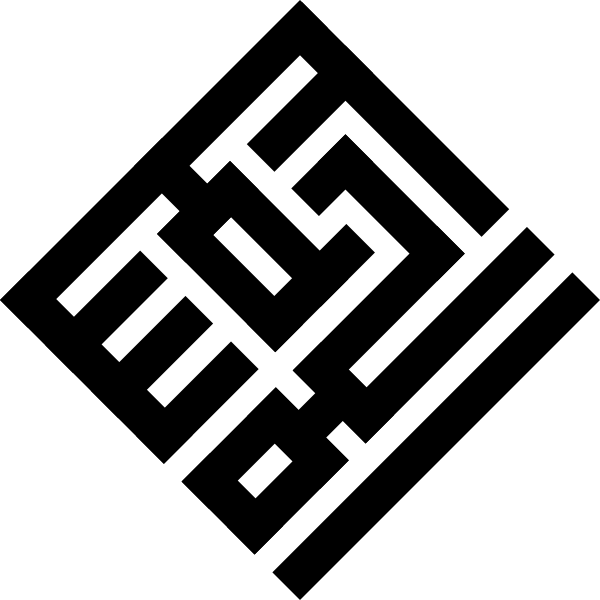
\includegraphics[width=0.1\textwidth]{img/alasaad-logo.png}\\
    Al Asaad\\
    \url{https://al-asaad.com}\\[-0.3cm]
    \url{https://al-asaad.vercel.app}
\end{center}
\tableofcontents\newpage
\listoffigures 
\chapter*{Abstract}
\addcontentsline{toc}{chapter}{Abstract}
This thesis presents a novel application of Statistics and Machine Learning techniques to analyze the Qur'\=an, complementing traditional methodologies while approaching the sacred text with appropriate respect and care. The research examines structural and linguistic patterns through multiple analytical lenses. Descriptive statistics reveal distinct clusters between \arb[trans]{makkiyyaT} \arb{makkiyyaT} and \arb[trans]{madaniyyaT} \arb{madaniyyaT} \arb[trans]{suwar} \arb{suwar}, with the latter demonstrating higher median values and greater variability. Morphological analysis of the root word \arb[trans]{Alh} \arb[novoc]{Alh} shows its common form \arb[trans]{'l-lahi} \arb[fullvoc]{'l-lahi} predominantly appears in \arb[trans]{madaniyyaT} \arb{madaniyyaT} chapters, while rarer forms (\arb[trans]{--|"'Alihati} \arb[fullvoc]{--|"'Alihati} and \arb[trans]{'alihatu} \arb[fullvoc]{'alihatu}) are exclusive to \arb[trans]{makkiyyaT} \arb{makkiyyaT} texts. Examination of manuscripts from 660-1000 CE from the Corpus Coranicum project confirms the preservation of these morphological patterns, supporting the integrity of oral transmission. For rhythmic analysis, the paper propose visualization techniques including line plots, heatmaps, rhythmic graphs, and histogram density plots, revealing strong patterns where approximately 70\% of \arb[trans]{'ayaT} \arb{'ayaT} endings feature transitions from short to long vowels. The paper further investigate concentric structures in \arb[trans]{sUraTu 'l-baqara} \arb{sUraTu 'l-baqara} using a novel Genetic Algorithm approach to objectively identify structural borders, employing CL-AraBERT for word embeddings with Cosine Distance metrics. The resulting optimal structural borders ($A$, $B$, $C$, $D$, $C^*$, $B^*$, $A^*$) were thematically analyzed using GPT-4o, confirming the concentric arrangement. This research demonstrates the value of computational methods, particularly the Julia programming language with libraries like QuranTree.jl and Yunir.jl, in revealing new insights into this complex, multi-layered text while respecting its sanctity and significance.

\chapter{Introduction}
\label{ch:introduction}
The use of scientific computing to studying the Qur'\=an is still in its early stage in the fields of Islamic Studies and Statistical and Machine Learning applications. This study will indeed benefit not only researchers from Islamic Studies but also Statisticians and Machine Learning researchers who are into text analytics. Having said that, it is therefore necessary to provide context to audiences of these disciplines to provide background on the state of Qur'\=anic studies and the increasing adoption of scientific methodology to studying humanities.
\section{Background}
The Qur'\=an or \arb[trans]{al-qur'An} \arb{al-qur'An} meaning \textit{the recitation}, the holy book of Islam, is revered by 1.9 billion (according to 2020 projection of \shortciteA[p.~13]{pewresearch}) Muslims across the globe as the literal words of God. Muslims believed that the Qur'\=an was gradually revealed (Qur'\=an 25:32) to Prophet Muhammad \arb{\arbmark{slm}} through angel \arb[trans]{jibrIl} \arb{jibrIl} or Gabriel (Qur'\=an 2:97). The Qur'\=an contains 77,429 Arabic words in total, which covers only 56 percent of the Greek New Testament which has 138,020 words in total \cite[p.~11]{sinai2017}. 

The Qur'\=an is divided into \textit{s\=urahs} \arb{sUr} which are the equivalent of chapters, each containing \arb[trans]{'ayAt} \arb{'ayAt} (meaning \textit{signs}), which are the equivalent of verses. The \textit{s\=urahs} \arb{sUr} are not arranged in chronological order as in the Bible's books and chapters, but rather arranged in monotonically decreasing length of number of verses after the first \textit{s\=urah} \arb{sUraT} (\textit{see} Figure \ref{fig:ayah_word_count}). The \textit{s\=urah} \arb{sUraT} of the Qur'\=an can be categorized into two types: the \arb[trans]{makkiyyaT} \arb{makkiyyaT} (Meccan) and \arb[trans]{madaniyyaT} \arb{madaniyyaT} (Medinan). The categories refer to the geographical location of where the \textit{s\=urah} \arb{sUraT} was revealed. Figure \ref{fig:ayah_word_count} shows the grouping of the \textit{s\=urahs} \arb{sUr}. Note that some of the \textit{s\=urahs} \arb{sUr} have mixed geographical locations\footnote{\textit{see} list of the location in \url{https://tanzil.net/docs/revelation_order}}, that is, a few of the \arb[trans]{'ayAt} \arb{'ayAt} in it were revealed in other geographical location apart from the geographical location of the rest of the \arb[trans]{'ayAt} \arb{'ayAt}. Therefore, the categorization in Figure \ref{fig:ayah_word_count} highlights the geographical location of the majority of the \arb[trans]{'ayAt} \arb{'ayAt} in the \textit{s\=urah} \arb{sUraT}.

\begin{figure}[!b]
    \centering
    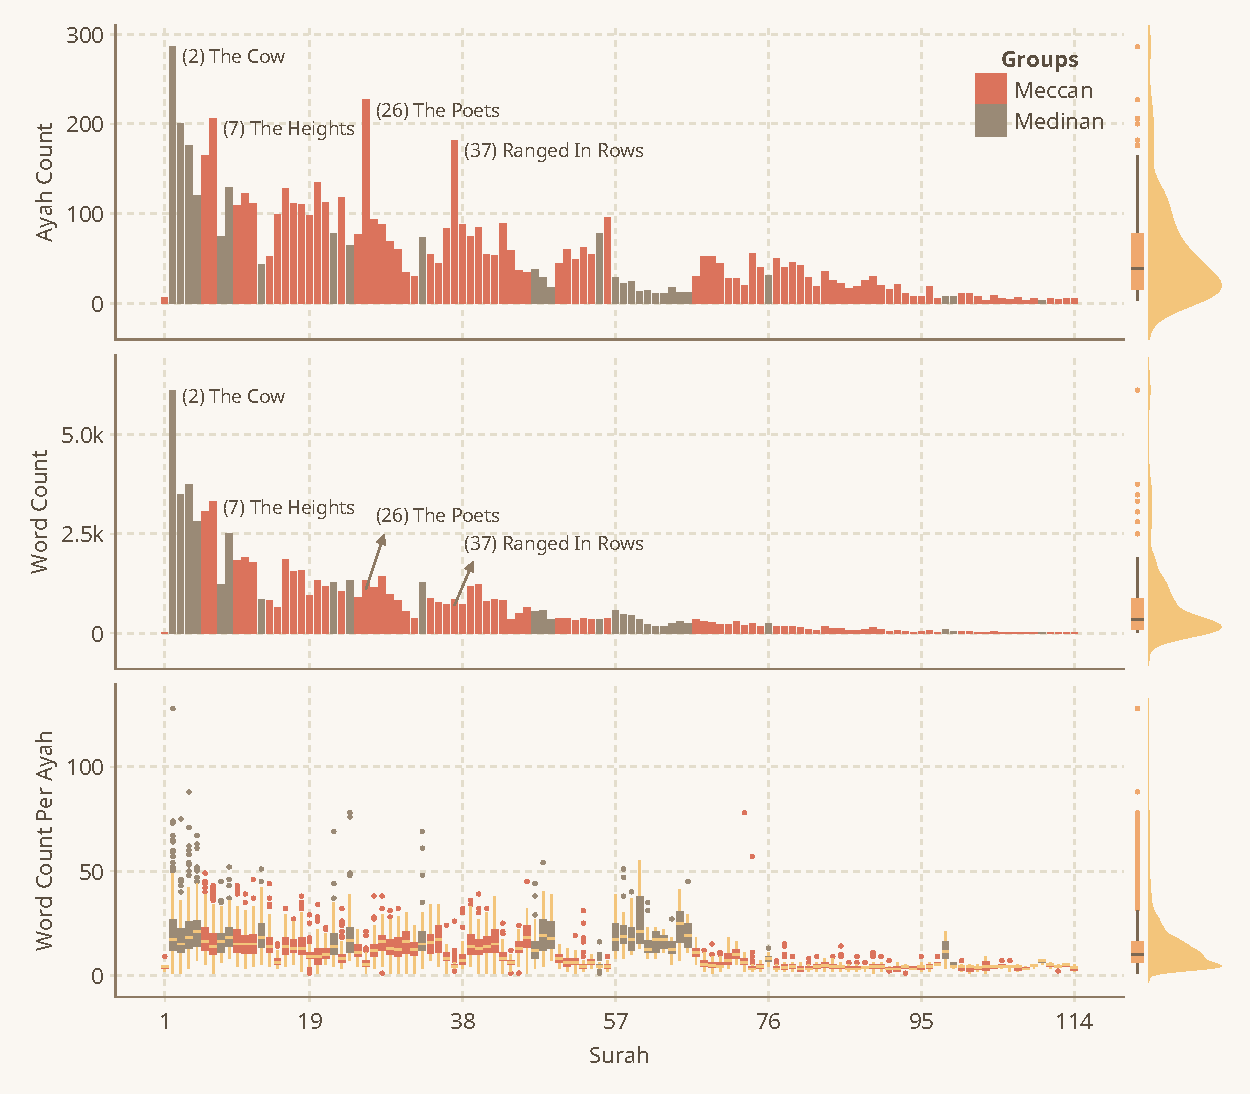
\includegraphics[width=\textwidth]{img/plot1.pdf}
    \caption{Statistics of the words and \arb[trans]{ayAt} \arb{ayAt} (verses) of the Qur'\=an}
    \label{fig:ayah_word_count}
\end{figure}

The Qur'\=an (meaning \textit{the recitation}) was revealed \textit{orally} by angel \arb[trans]{jibrIl} \arb{jibrIl} to Prophet Muhammad \arb{\arbmark{slm}} and passed onto other believers through oral tradition (reciting the Qur'\=an to students repeatedly so as to memorize it, instead of writing it down and let the believers read it and memorize it). Memorizing 77,429 Arabic words of the Qur'\=an through oral transmission can be a difficult task, but what aids this memorization is the rhythm feature of the Qur'\=an. According to one Orientalist, \citeA{sinai2017}, "rhyme, however, or rather a periodically recurrent word-final assonance, is a feature of the Qur'\=an throughout, and it naturally partitions the \textit{s\=urah} \arb{sUraT}." Indeed, because of this feature, it makes it easy to memorize the entire Qur'\=an, and the one who do so is called \arb[trans]{hafi.z} \arb{hafi.z} meaning \textit{one who remembers} or \textit{keeper}. Qur'\=an memorization contest is a common event in Muslim countries, the Philippine embassy has hosted one in 2022 in Saudi Arabia \cite{mb2022}.

According to the Muslim tradition, the oral transmission of passing the Qur'\=an from a \arb[trans]{hafi.z} \arb{hafi.z} to new believers was gradually put into writings as requested by the believers themselves. The idea was brought up after the battle of Yamama, where many of the Muslims who died were \arb[trans]{qurrA'} \arb{qurrA'} (\textit{the one who properly recite the Qur'\=an}), and so fearing that their numbers will reduce in other battle fields, Umar ibn al-Khattab \arb{`umaru bnu 'l-xa.t.tAb} (who became the second caliph) suggested to the first caliph, Ab\=u Bakr 'Abd All\=ah ibn 'Ab\=i ibn 'Ab\=i Qu\d{h}\=afa, \arb{'abU bakriN `abdu 'l-lAhi 'ibni 'abiY qu.hAfaTa} or short for Ab\=u Bakr \arb{'abU bakr}, to collect the Qur'\=an into writing. Ab\=u Bakr then authorized Zaid ibn Thabit \arb{zaydi bni _tAbitiN} for the task. According to Zaid, he started collecting from the leafless stalks of the date-palm tree and from the pieces of leather and hides and from the stones, and from the chests of men (who had memorized the Qur'\=an, i.e. the \arb[trans]{hafi.z} \arb{hafi.z})\footnote{\textit{see} \url{https://sunnah.com/bukhari:7191}}. Long story short, the effort was finally codified by the third caliph, Uthman ibn Affan \arb{`u_tmAnu bnu `affAn} in the year 645 CE, which was then recopied and distributed to the different regional capitals of the early Islamic empire of that time. The rest of the copies outside this codification were then burned\footnote{\textit{see} \url{https://sunnah.com/bukhari:4987}} down in order to have one standard Qur'\=an. The Qur'\=an nowadays is therefore assumed to be based on Uthmanic codex because of the story mentioned. That is, if indeed Uthman has ordered to burn other copies of the Qur'\=an outside his codification, then what's left should only be based on his codex or archetype, and that should only be the inherited codex of the Muslims today.

The Qur'\=an is believed by the Muslims to have been preserved since it was first recited by angel \arb[trans]{jibrIl} \arb{jibrIl} or Gabriel to the Prophet \arb{\arbmark{slm}}. Many orientalists had been skeptic about this claim, for example, John Wansbrough theorized that the Qur'\=an was collected over a 200-year period \cite<\textit{see}>[p.~101]{wansbrough2004} after the death of the Prophet \arb{\arbmark{slm}}, instead of within a few years after the death of the Prophet \arb{\arbmark{slm}}. However, recent findings through radiocarbon dating brings forward strong evidence of potential preservation of the whole Qur'\=an, which the Muslims believed to be so. For example, the Birmingham Qur'\=an manuscript discovered in 2015 is dated to be between 568 and 645 CE with 94.5\% accuracy, making it among the oldest Qur'\=anic manuscript in the world \cite<\textit{see} >{bu2015}. Its predicted range of years intersects with the lifetime (570 to 632 CE) of the Prophet \arb{\arbmark{slm}}. What is interesting is that the Birmingham Qur'\=an is consistent with the Qur'\=an today, word-by-word and letter-by-letter\footnote{The orthography of the Arabic letters in the early days had no diacritics and were written in its basic consonantal skeleton. That is, Arabic orthography and grammar were in their nascent when the Qur'\=an was revealed, and therefore has to adjust and catch up, to capture and preserve the proper recitation of the Qur’an.}, see Figure \ref{fig:birmingham}. This is indeed another evidence that the Qur'\=an today was codified by Uthman since the discovery of the Birmingham Qur'\=an manuscripts have confirm it. In addition to this, the Sana'a Palimphest is also among the oldest Qur'\=an radiocarbon dated to be between 578 CE and 669 CE with 95\% accuracy \cite{behnam2010}, which according to \citeA{sinai2017}, "neither does the edited portion of the Sana'a palimpsest offer evidence for additional or missing verses or for a divergent verse order within the \textit{s\=urahs} \arb{sUr}." Given these discoveries on the recent Quranic manuscripts, the claim of \citeA[p.~101]{wansbrough2004} is now untenable \cite<\textit{see}>{sinai_2014}.

\begin{figure}[!b]
    \centering
    \includegraphics[width=\textwidth]{img/birmingham.jpg}
    \caption{20th Century Qur'\=an (left) in its fully featured orthographies vs Birmingham Qur'\=an dated between 568 and 645 CE (right) in its basic consonantal skeleton. Image from \protect\citeA{wikibirmingham}.}
    \label{fig:birmingham}
\end{figure}

One likely reason as to why the scribes were able to preserve the Qur'\=an in the two folios of the Birmingham Qur'\=an manuscripts follows from the fact that the Qur'\=an is firstly memorized before it was decided to be written. So that, the \mbox{Topkapi} manuscripts that contain 99\% (only 23 verses missing)---dated around 701 to 750 CE \cite{karatay1962}\footnote{\textit{see also} \url{https://corpuscoranicum.de/en/manuscripts/1977/page/1-410?sura=1&verse=1}}, that is, around 69 to 118 years after the death of the Prophet \arb{\arbmark{slm}}---of the Qur'\=an today was likely partly written from memory. This is possible since the Qur'\=an possesses a rhytmic feature (that aids with memorization) that naturally divides its verses or \arb[trans]{'ayAt} \arb{'ayAt}, and that the Qur'\=an memorization competition is still held to this day \cite<as in the example of >{mb2022}, apart from the fact that it needs to be recited (any chapter after the first chapter of the Qur'\=an according to the choice of the worshipper) every prayer from memory. Bottomline, there are many avenues for Qur'\=an recitation from memory, and these have helped in its preservation. Moreover, since there are no significant evidence of insertion or malicious intention on addition or revision in all of the extant Qur'\=anic manuscripts so far, some Orientalists came up with other theories of insertions on the basis of the literary style of the Qur'\=an, see for example \citeA[p.~92]{sinai2017}, where verse 102 of \arb[trans]{sUraT 'l-.sAffAt} \arb{sUraT 'l-.sAffAt} or The Chapter of \textit{Ranged in Rows} is theorized as addition because it is longer compared to other verses in the said chapter, refer to \citeA[p.~92]{sinai2017} for his other reasonings. Nonetheless, the Qur'\=an is indeed stable based on the extant manuscripts.

Furthermore, the vastness of the early Islamic empire meant that different Muslim regional capitals have covered populations with different Arabic dialects, and so to accommodate these differences, Muslims believed that there were seven variant readings of the Uthmanic codex. Variant readings are defined as different pronunciations of the same word, in this case seven Uthamnic Qur'\=an for seven different pronunciations. The \arb[trans]{.hadI_t} \arb{.hadI_t} or \textit{narration} comes from Ubayy ibn Ka'b \arb{'ubayyi bin ka`b} who reported\footnote{source: \url{https://sunnah.com/muslim:821a}} that the Prophet \arb{\arbmark{slm}} was near the tank of Banu Ghifar that \arb[trans]{jibrIl} \arb{jibrIl} or Gabriel came to him and said: "... Allah has commanded you to recite the Qur'\=an to your people in \textit{seven dialects}, and in whichever dialect they would recite, they would be right." Recent work of \citeA{sidky2020} shows that the material evidence on the regional variants is in remarkable agreement with well-attested written variants documented in the traditional Muslim literature.

Muslim and non-Muslim scholars alike have been extremely interested in understanding the unique literary characteristics of the Qur'\=an. As mentioned earlier, unlike other books like the Bible (arranged in chronological order), the Qur'\=an does not follow any obvious organization. In addition to this, a \textit{s\=urah} \arb{sUraT} does not fit the exact definition of a chapter. Indeed, the name attached to a \textit{s\=urah} \arb{sUraT} is often decided as the unique entity mentioned in the said \textit{s\=urah} \arb{sUraT}, its main purpose is to help early Muslims distinguish which \textit{s\=urah} \arb{sUraT} they are talking about, this is contrary to the chapter name where the associated name is obviously the main topic of the chapter. Further, as described by \citeA{sinai2017}, "... the compositional unity of the long surahs located at the beginning of the corpus is anything but obvious: at least at first sight, they can appear a flit back and forth between different topics in a largely haphazard manner. This impression is not limited to Western readers: even pre-modern Muslim scholars have often approached their scripture as a quarry of unconnected verses and groups of verses that bear little intrinsic relation to what precedes and follows." It wasn't until \citeA{Neuwirth_2007}, that the compositional unity of the Qur'\=an can be observed in tighter literary unities, as \citeA{Neuwirth_2007} showed that the many of these texts display a tripartite structure and are often constructive around a narrative middle part \cite{sinai2017}. Samples of the organizational style of the Qur'\=an was shown in \citeA[p.~88]{sinai2017}.

\section{Rationale of the Study}\label{sec:rationale}
Attempts at understanding the Qur'\=an by Qur'\=anic scholars were mostly done with the use of manual processes, that is, studying the scriptures by going through its content one-at-a-time manually. However, with the advent of computers, some researchers have started using it to aid in their study. The first known to have used computers for studying the Qur'\=an was likely Rashad Khalifa in 1968\footnote{\textit{see} \url{https://www.masjidtucson.org/quran/miracle/a_profound_miracle_sura68nun133.html}}, where he studied the significance of the mysterious initials at the beginning of some \textit{s\=urahs} \arb{sUr}. Rashad uploaded the Qur'\=an into his computer by transliterating the Arabic letters and other Qur'\=anic orthographies into Roman letters and symbols that the computer can easily parse. This approach of using computers to find new insights is more common in the field of science, and it was new to the field of Qur'\=anic studies.

Indeed, to proceed with the use of scientific computing, the Qur'\=an will be treated as the data that needs to be analyzed using what is called Natural Language Processing (NLP), a branch of Machine Learning (ML) that aims to understand natural languages, such as Arabic. To instruct the computer to do Statistical analyses, ML, or NLP, one needs to use a \textit{software application} or a formal language called \textit{programming language}. There are several programming languages that the computer can understand. The popular one for researchers in the field of sciences are Python, R, and sometimes Julia \shortcite{Julia2017}. These programming languages will be used to construct instructions for computer. Therefore, if the data is the Qur'\=an, then there should be a way to interface with it using any of these programming languages. Or alternatively, there should be a way to upload it into the chosen programming language and encode the Arabic letters into something that can be easily parsed by the computer, like what Rashad \mbox{Khalifa} did. Having said that, there are indeed some programming languages with libraries or packages for interfacing with the Qur'\=an, and this is true for Python, R, and \mbox{Julia}. For this study, Julia programming language since its  library for interfacing the Qur'\=an using the QuranTree.jl\footnote{\textit{see} \url{https://alstat.github.io/QuranTree.jl/stable/}} has more features compared to those available in R and Python \cite<\textit{see}>{asaad2021qurantree}. QuranTree.jl is based on Tanzil\footnote{\url{https://tanzil.net/download/}} for the Qur'\=anic Arabic texts, and \citeA{dukes-habash-2010-morphological} for morphological annotation, which both libraries from R and Python do not have in terms of morphological annotation from \citeA{dukes-habash-2010-morphological}.

Now that the programming language for this paper is identified, next is to understand how Statistics and Machine Learning can help in studying the Qur'\=an. Statistics is a branch of Science that aims to study features or characteristics of data generated from a random phenomenon. The findings of Statistical analyses can then be used to make conclusions or predictions of the general population of the data or general characteristics of the data. Machine Learning or ML, on the other hand, is a branch of Artificial Intelligence that heavily intersects with Statistics, albeit with distinct differences as well. Both Statistics and ML aims to characterize data by learning its features, but ML research aims on complex models that are often inspired by simpler models from Statistics. Therefore, one can think of Statistics as one of the fundamentals of ML. 

One of the goals of Statistics and Machine Learning is to summarize all of the learned features into a hypothesized equation or hypothesized mathematical formula whose parameters or weights are optimized to capture the most characteristics of the data. It is called hypothesized equation since the researcher is the one who decide which family of equation best describe the characteristics of the data. The said equation is called a \textit{model}. Therefore, a model is a generic entity that can be fitted or molded to capture the features of the data. Mathematically and in general, a model can be written as:
\begin{equation}\label{eq:general_model}
    \hat{y}:=h(x|\mathbf{\theta}),
\end{equation}
which is a mapping between the sets $\mathcal{X}$ and $\mathcal{Y}$ where $x\in\mathcal{X}$ and $y\in\mathcal{Y}$ through a hypothesized function $h$. The idea of modeling is to find the optimal value of $\mathbf{\theta}$ in such a way it will minimize the error between the actual data (represented by $y$ below) and the predicted one $\hat{y}$:
\begin{equation}
    \varepsilon:=y-\hat{y}=y-h(x|\mathbf{\theta}).
\end{equation}

To help understand the concept of modeling, and relate it to the fashion industry, which the author assumes most readers are familiar with, a model in a fashion industry is responsible for representing the characteristics of the target customers (in Eq. \ref{eq:general_model} this is $y$). Therefore, for a clothing company, they hire Asian models (in Eq. \ref{eq:general_model}, this is $\hat{y}$ or $h(x|\mathbf{\theta})$) to target Asian customers (in Eq. \ref{eq:general_model} this is $y$). So that, when these models wore the clothes sold by the said company, the potential customer will more or less be able to relate to the model, and be able to imagine themselves wearing that same clothes as well, which help them incline to buying the said clothing. The model, therefore, does not necessarily have the looks of every target Asian customers, but at least in terms of height, skin tone, hair, and other common Asian features, the model will likely have it, or at least the difference is more or less minimal (in Eq. \ref{eq:general_model}, the difference is represented by $\varepsilon:=y-\hat{y}$). The question now is, what are the benefits that this model can bring to the clothing company? Well, the clothing company will be able to create products that are tailored to their Asian customers using the said model, since the company will have the right baseline measurements needed. Relating this analogy to the technical concept discussed earlier, you can think of the target customers as the
real or actual data (in Eq. \ref{eq:general_model} this is $y$), and the model as the same technical term use in Machine Learning and Statistics (in Eq. \ref{eq:general_model} this is $h(x|\mathbf{\theta})$), but this time this technical model is expected to capture the characteristics of the real data analogous to fashion model that is expected to capture the characteristics of the target customer. This Statistical or Machine Learning model brings the following benefit: researchers will be able to study the real data by simply using the model to answer questions that are not available in the sampled real data.

In this paper, the aim is to make use of the Statistical or Machine Learning modeling to understand the characteristics of the Qur'\=an in terms of the morphologies of its canonical text in its modern orthography. More specifically, the following are the general objectives:

\section{Objectives}\label{sec:objectives}
The following are the general and specific objectives of this paper:
\begin{enumerate}
    \item What are the structural characteristics of the Qur'an that can be extracted from its rich morphologies using statistical and large language models?
    \begin{enumerate}
        \item What are the statistics of the Qur'\=an's morphological features in terms of its parts of speech and selected entities like God's name and the prophets names mentioned?
        
        \item How do the rhythmic signatures of the Qur'\=an of the verses looks like and what are statistical insights that can be extracted?
        
        \item What are the supporting statistical insights on the current divisions of the Qur'\=an's verses? 
    \end{enumerate}
    
    \item What other insights that can be extracted from the semantics of the Qur'an's texts using statistical and large language models?
    \begin{enumerate}
        \item How does the theory of \textit{concentrism} be formulated statistically, and what are the insights from the statistical and large language models on this? 
        
        \item How do the surahs are organized in terms of the topics? What are the themes that can be extracted for each of the surahs?
        
        \item How do these extracted themes compare to the summaries of Abdel\linebreak Haleem's English translation of the Qur'an?
    \end{enumerate}
    
    \item How does this combination of statistical, machine learning, and artificial intelligence with the Muslim's traditional literatures help in understanding the Qur'\=an, especially with the advent of Generative AI?
\end{enumerate}

\section{Significance of the Study}\label{sec:significance}
While the Qur'\=an has been extensively studied by Muslims and non-Muslims scholars alike, especially in the topic of Meccan and Medinan surahs, there is still a lot to uncover from the perspective of Computational Statistics. Hence, the significance of this study is that it brings forward new ways of extracting insights from the Qur'\=an by leveraging Computations, Statistics, Machine Learning, and AI, that is still in its early stage in the field of Qur'\=anic Studies. Therefore, this new perspective or process of studying the scripture not only aids the scholars of the Islamic Studies, but may also contribute indirectly to community development and policy makers who use Qur'\=an as part of their decision making.
\section{Scope of the Study}
The paper will cover all chapters of the Qur'\=an both for the Morphological and Topic Modeling analyses, but it will only present the results of \textit{s\=urahs} \arb{sUr} with at least 1000 words. The rest of the result will be part of the web application that can be used to query the Qur'\=an. It will also not delve into the \textit{tafsir} \arb{tafsIr} of each of the verses, but only when necessary for further context.
\section{Thesis Organization}
The paper is organized as follows: Chapter 2 will discuss the related literatures, Chapter 3 will discuss the methodology, Chapter 4 will present the results and discussions, and finally Chapter 5 will contain the conclusion and recommendation. The references and appendices are placed after the Chapter 5.
\chapter{Review of Related Literature}\label{ch:rrl}

As mentioned in the previous chapter, the earliest paper on Qur'\=anic studies using computer was likely the work of Rashad Khalifa in 1968\footnote{\url{https://www.masjidtucson.org/quran/miracle/a_profound_miracle_sura68nun133.html}}, which led to one of his book entitled `The Computer Speaks: God's Message to the World' (\textit{see} \citeA{rashad1981}). While the work of Rashad started at studying the mystery letters in the beginning of some \textit{s\=urahs} \arb{sUr} (for example Qur'\=an 2:1, 3:1, 7:1, etc.), it quickly went on to cover what he calls other \textit{mathematical miracles}, all of which are covered in \citeA{rashad1981}. His work were mainly based on counting the positional statistics of selected entities like names of God relative to other names or words in the Qur'\=an, and showing through counting and simple math of factoring some totals, he showed an interesting matches among these statistics. He was able to do this by transliterating the Qur'\=an into Alpha-Numeric typesets for easy parsing of the computers back then. His findings led him to generalize the claim that God revealed His words through this "mathematical" patterns throughout the Qur'\=an, and that those verses that were off and did not conform to this discovered "mathematical" patterns led him to extensive investigation of the said verses, and concluded that those could be or surely be an insertion that should not have been in the Qur'\=an in the first place. There are two verses that were off according to Rashad, and he called these verses as \textit{false verses}\footnote{\url{https://submission.org/App24.html}}, these are the last two \arb[trans]{'AyAt} \arb{'AyAt} of \arb[trans]{sUraTu 'l-tAwbaT} \arb{sUraTu 'l-tAwbaT} or The Chapter of \textit{Repentance}. These two verses were removed in Rashad's Qur'\=an translation\footnote{\url{https://www.masjidtucson.org/quran/frames/}}. Rashad believed so much on his findings that he self-proclaimed himself to be a messenger\footnote{\url{https://www.masjidtucson.org/submission/faq/rashad_khalifa_summary.html}} with this new findings and that the Qur'\=an nowadays should conform to his found "mathematical" patterns. This self-proclamation led to his assassination.

What the above tells us is that early on with the advent of computers, there was already interest in trying to understand the structural characteristics of the Qur'\=an. This is because the Qur'\=an is not like the Bible that is arranged chronologically, but rather arranged in generally decreasing number of \arb[trans]{'AyAt} \arb{'AyAt} per \arb[trans]{sUraT} \arb{sUraT} as shown in Figure \ref{fig:ayah_word_count}. This unique structure led to different literatures on understanding the Qur'\=an's design in terms of its unique presentation of topics, not only from the Islamic studies researchers but also computer scientists who were into Arabic Natural Language Processing studies. 

Among the pioneers in computational applications for the Qur'\=an is the work of \shortciteA{thabet2004}, who built a stemmer system for the Qur'\=an. A stemmer system is a system for trimming inflected words into its basic form, which grammatically mean its the root form. For example, in English language the root word for \textit{computational}, \textit{computer}, \textit{computation}, and \textit{computerize} is \textit{compute}. Therefore, the root of a word forms different \textit{stems} representing the different words. Hence, the idea of stemming is to trim these words into its basic form, so that it would be easy to do word clustering or grouping through word similarity. According to \citeA{thabet2004}, the rich morphology of the Qur'\=anic language or the Classical Arabic makes it even more difficult to do word stemming. Moving on, \citeA{thabet2005} builds on top of this stemming system, and used it for tokenization of the Qur'\=anic words, and building a statistical methodology for clustering or grouping the chapters of the Qur'\=an, in particular \citeA{thabet2005} used a Agglomerative Hierarchical Clustering based on the Euclidean distance of the adjusted word frequency of a \arb[trans]{sUraT} \arb{sUraT}.

The work of \citeA{thabet2004} and \citeA{thabet2005} used a Qur'\=an's corpus that was transliterated to Roman letters and symbols. Indeed, with the growing interests on studying the Qur'\=an from the lense of Data Analysis and Natural Language Processing, resulted into creating digital corpi of the Qur'\=an that captures the different aspects of its linguistic styles. Hence, a series of work by Sharaf and Atwell led to the following publications: \shortciteA{sharaf2009} studied knowledge representation of the Qur'\=an's verb valences using FrameNet frames, the output of which is a lexical database as a corpus of Qur'\=an's verbs. Further, the work of \shortciteA{sharaf2012} came up with corpus for the annotations of the Qur'\=anic pronouns, the authors named it as QurAna. Building on this work, \shortciteA{sharaf2012b} came up with a corpus for studying Qur'\=anic relatedness based on the commentary of Ibn Kathir \arb{ibn ka_tir}, the authors named this corpus as QurSim. Apart from Sharaf and Atwell, Dukes and Habash was also working on this, but specifically on the morphological annotations. The final and verified\footnote{The authors used online community collaboration for checking or verification of the morphological annotations. This was necessary since the Qur'\=an is a highly regarded book by Muslims, and there should be no mistakes in annotations.} work of the authors is the \shortciteA{dukes-habash-2010-morphological}, which also led to other publications \shortcite{dukes2010online, dukes2013supervised, dukes2010dependency} related to this.

With the establishment of a morphological annotated corpus for the Qur'\=an, the hoped was to have further analyses on the said scripture using statistical and machine learning methodologies. As such, the work of \shortciteA{dukes-habash-2011-one, dukes2015statistical} were among the first to do so, where they constructed a statistical parser through machine learning. This was then followed by \shortcite{siddiqui2013} who used the said corpus for topic modeling using Latent Dirichlet Allocation, the said study started with 114 \arb[trans]{sUwar} \arb{sUwar}, but after processing it went down to 24 \arb[trans]{sUwar} \arb{sUwar} after considering \arb[trans]{sUwar} \arb{sUwar} with 1000 or more words. This was mainly due to the very sparse document term matrix for the Term Frequency - Inverse Document Frequency\footnote{\textit{See} Section \ref{sec:tf-idf}} (TF-IDF) embedding if considering all of the 114 \arb[trans]{sUwar} \arb{sUwar}. Aside from this, the rest have used the corpus by \shortciteA{dukes-habash-2010-morphological} as part of benchmark for morphological analysis or for new lexicographic database, for example \shortciteA{sabtan2017morphological, jarrar-hammouda-2024-qabas-open}.

For the case of \textit{rhythmic analysis} of the Qur'\=an, most of the literatures have looked into the recitation of this rhythmic feature of the Qur'\=an, for example the work of \shortciteA{shekha2013effects, samhani2022rhythms, abdullah2011effect} and \shortciteA{naqvi2020effect} have all investigated the effect of listening to the Qur'\=an recitation on temporal Electroencephalogram (EEG) signals and on human physiology through Electrocardiogram (ECG) signal. The work of \shortciteA{shekha2013effects} subjected 11 students to listen to soft music, hard music, and Qur'\=anic recitation and collected the \textit{alpha} wave signals of it in EEG. The authors used t-test and ANOVA to compare the results from the three input audio. Their findings suggest that the Qur'\=an recitation both during opened eyes or closed eyes while listening to the Qur'\=an have significant magnitude in \textit{alpha} waves electrode. The same study was also conducted by \shortciteA{samhani2022rhythms}, but this time listening to Arab News; Qur'\=anic recitation of \arb[trans]{sUraTu 'l-fAti.haT} \arb{sUraTu 'l-fAti.haT}; and simply resting, that is not listening to any audio. The authors used Analysis of Variance (ANOVA) and Hierarchical Clustering for the resulting Beta oscillation data. Their study found that the said Beta rhythms synchronization
of listening to \arb[trans]{sUraTu 'l-fAti.haT} \arb{sUraTu 'l-fAti.haT} is associated with verbal fluency, academic performance, social
interaction, inhibitory function, movement planning, self-motivation, self-management and
reactivation of sensory features of memory trace as highly activated cluster, followed by working memory, language processing and decision making as medially activated cluster. Another similar study was also done by \shortciteA{abdullah2011effect} with same pattern of output, and that is a good effect on the EEG of the patients. On the other hand, the work of \shortciteA{naqvi2020effect} investigated the effect of the Qur'\=an on the ECG. The authors used different classification models for classifying signals from the Qur'\=an listening. 

While the rhythmic feature is the most obvious feature of the Qur'\=an, the structural arrangement of the topics and verses are not as obvious as compared to any other books. Hence, there have been several attempts to understand these arrangements even from the pre-modern day Muslim scholars. The Basran writer al-Jahiz (d. 255/868 or 869) produced a work entitled \textit{The Composition of the Qur'an}, even a scholar named Abu Bakr al-Nisaburi from 4 AH/10 CE would ask such questions as, "Why is this verse next to the other one?" and, "What is the widom in the plcement of this chapter next to this other one?" \shortcite{farrin2014structure}. According to \shortciteA{farrin2014structure}, since the 1980s, numerous scholars in the field have followed their lead and have begun to show clearly that individual chapters, both short and long, are indeed characterized by a high degree of unity. With that said, among the structure that was found is the \textit{theory of concentrism}, which accordingly is the structural pattern of the Qur'\=an. This was the proposition of Michael Cuypers\footnote{All of his work are written in French. Please refer to \shortciteA{farrin2014structure} for the list of articles written by Cuypers.}. As far as the knowledge of the author, the most comprehensive exposition of the theory of \textit{concentrism} in English is the work of \shortciteA{farrin2014structure}. However, not a single paper have been written for a mathematical formulation of this that can be used for statistical analyses. 

Finally, the recent advancement of large language models (LLM) and its use for the retrieving information resulted into what is called the Retrieval-Augmented Generation (RAG) proposed by \shortciteA{lewis2020retrieval}. This recent methodology have been used by \shortciteA{alan2024rag} for developing the MufassirQAS LLM by augmenting the OpenAI's Application Processing Iterface (API) for GPT3.5 Turbo with vector database of Islamic sources. The same process will be used but this paper augments the generation of the LLM using the results from the rhythmic analysis and concentrism theory, which both have not been integrated to any RAG applications.
\chapter{Background on Probability and Statistics}\label{ch:statistics}
This chapter will discuss some statistical concepts that will be used to understand and build up the ideas behind the methodology of this paper, which is presented in the next chapter. With that said, the discussions are organized as follows: Section \ref{sec:descriptive_stat_method} will present the concept of Descriptive Statistics; Section \ref{sec:probability_method} will discuss the Probability Theory; and, Section \ref{sec:stat_graphs_method} will discuss the Statistical graphs or plots.

Further, the topics discussed here may be self-explanatory for Statisticians, ML researchers or those with Mathematical background. However, for the benefit of readers coming from humanities background, the paper will present the methodology as follows: mathematical formulas are formalized for purpose of brevity through Definition, Proposition, and Corollary, but immediate to these are explanations or examples aimed to be simple enough for non-statistician readers. As a guide, statisticians or ML researchers can simply read the Definition, Proposition, and/or Corollary. Whereas for humanities readers, the reading shouldn't not stress too much on the said mathematical formalities, and instead proceed to the discussions or examples immediate to it to aid with the understanding.
\section{Descriptive Statistics}\label{sec:descriptive_stat_method}
Among the basic statistical methodologies for summarizing information or data is what is known as Descriptive Statistics. From the name itself, these statistics are meant to convey simple descriptions of the data. For example, \textit{mean} and \textit{variance} are common statistics used for describing the data. The formulas for these statistics are given in the following definitions:
\begin{defn}[Mean]\label{defn:mean}
Let $x_i, i\in\{1,\cdots,n\}$ where $n\in\mathbb{N}$, then the \textit{mean} of $x_i$s is defined as follows:
\begin{equation}
    \bar{x} = \sum_{i=1}^n x_i, \qquad\text{where}\;x_i \in\mathbb{R}.
\end{equation}
\end{defn}
\begin{defn}[Variance]
    Let $x_i, i\in\{1,\cdots,n\}$ where $n\in\mathbb{N}$ and let $\bar{x}$ be the mean defined in Defn. \ref{defn:mean} then the \textit{variance} of $x_i$s is defined as follows:
    \begin{equation}
        \mathbb{V}\text{ar}(x) = \frac{1}{n-1}\sum_{i=1}^n (x_i-\bar{x})^2, \qquad\text{where}\;x_i \in\mathbb{R}.
    \end{equation}    
\end{defn}
\begin{defn}[Standard Deviation]
Let $\sigma^2$ be the variance, then the standard deviation, denoted by $\sigma$, is defined as $\sigma:=\sqrt{\sigma^2}$, that is, square root of the variance.    
\end{defn}
The mean is simply the average of the data points, while the variance is a single number that measures or summarizes the distances of the data points from the mean. The variance therefore measures how spread or varied the data points are. In practice, however, standard deviation is more popular for measure of variability since it doesn't get big easily due to the square root operator. Standard deviation is also the preferred metric for this paper.
\section{Probability Theory}\label{sec:probability_method}
Statistics is built around the concept of Probability Theory. Hence, it is important to understand how this mathematical theory behind the statistical concepts work. Probability theory is a discipline in itself. It is a branch of mathematics that aims at studying realizations or observations from random phenomena. It does this by using algorithms and models (\textit{see} discussion in Chapter \ref{ch:introduction} for understanding the model). These probability models are mathematical formula design to characterize or describe the patterns of data points. The simplest form of these models is the univariate probability density functions. However, before discussing these models, the idea behind it should be build up from ground up so that humanities readers can appreciate it. To do this, the discussion will proceed with the concept of probability.
\begin{defn}[Probability]\label{defn:probability}
A probability is a mathematical concept that measures the likelihood or chance of some event to happen.
\end{defn}
Indeed, this idea of probability is well known or is easily understood by many. So that, the probability that someone will die is 1, meaning 100\%, since that's how natures and biology work. Further, the probability of selecting one \arb[trans]{'ayAt} \arb{'ayAt} from \arb[trans]{sUraT 'l-fAti.hati} \arb{sUraT 'l-fAti.hati} through a random draw is one out of seven, assuming each \arb[trans]{'ayAt} \arb{'ayAt} has equal chances of being drawn.

Now, to gradually formalize the concept into mathematics, the succeeding definitions will be discussed to build up the definition of a probability distribution.
\begin{defn}[Sample Space]
Let $\omega_1,\cdots,\omega_n, \forall n\in\mathbb{N}$ be the list of all possible outcomes of a random event or a phenomena, then the sample space, denoted by $\Omega$, is defined as the collection of all these possible outcomes including the empty set denoted by $\emptyset$.
\end{defn}
\begin{exmp}\label{ex:sample_space}
Consider the random phenomenon or event where someone randomly picks a verse from the Qur'\=an, what is the probability that it will be a Meccan \arb{makkiyyaT} or a Medinan \arb{madaniyyaT} verse?

The possible output for such random event is either Meccan or Medinan. Suppose, we let Meccan to be denoted by $\omega_1$ and Medinan to be denoted $\omega_2$, then the sample space, which is the collection of all possible output is denoted as follows:
\begin{equation}\label{ex_eq:sample_space}
    \Omega:=\{\text{\arb{makkiyyaT}},\text{\arb{madaniyyaT}}\}=\{\text{Meccan}, \text{Medinan}\}=\{\omega_1,\omega_2\}
\end{equation}
It should be understood that $\emptyset$ is also included in $\Omega$, but is not written for brevity.

\end{exmp}
\begin{defn}[Event]
Let $\Omega=\{\omega_1,\cdots,\omega_n\}, \forall n\in\mathbb{N}$, be the sample space, then an event, denoted here as $\mathscr{A}$, is defined as the subset of the sample space, i.e., $\mathscr{A}\subseteq{\Omega}$.
\end{defn}
\begin{exmp}
From Ex. \ref{ex:sample_space}, consider drawing two samples from the Qur'an, what is the sample space and give an example of a possible event?\\
\textit{Solution:} The sample space is given below:
\begin{align}
    \Omega=&\{(\text{\arb{makkiyyaT}},\text{\arb{makkiyyaT}}),(\text{\arb{makkiyyaT}},\text{\arb{madaniyyaT}}), (\text{\arb{madaniyyaT}}, \text{\arb{makkiyyaT}}), (\text{\arb{madaniyyaT}}, \text{\arb{madaniyyaT}})\}\nonumber\\
    =&\{(\text{Meccan},\text{Meccan}),(\text{Meccan},\text{Medinan}), \\
    &\;\;(\text{Medinan},\text{Meccan}), (\text{Medinan},\text{Medinan})\}\\
    =&\{(\omega_1,\omega_1),(\omega_1,\omega_2),(\omega_2,\omega_1),(\omega_2,\omega_2)\}
\end{align}
So that, if $\mathscr{A}$ is the event of drawing two \arb[trans]{'ayAt} \arb{'ayAt} from the Qur'\=an, then a possible event is given by 
\begin{equation}
    \mathscr{A}:=\{\text{\arb{madaniyyaT}}, \text{\arb{makkiyyaT}}\}=\{\text{Medinan}, \text{Meccan}\}=\{\omega_2,\omega_1\}
\end{equation}
Therefore, $\mathscr{A}\subseteq\Omega$, read as $\mathscr{A}$ is a subset of $\Omega$.
\end{exmp}
Now, going back to the discussion on the concept of probability above and reflect on the example given, that the probability that someone will die is 1; and that the probability of selecting one \arb[trans]{'ayAt} \arb{'ayAt} from \arb[trans]{sUraT 'l-fAti.hati} \arb{sUraT 'l-fAti.hati} through a random draw is one out of seven. It therefore begs the following questions: how does one solve this? Like how does it translate into a formal mathematical computation?

Indeed, to appreciate the motivation of the succeeding definitions, it is important to devise a logical approach to computing probability mathematically, and this should explain why the following definitions are defined the way they are.

Probability as already defined in Defn. \ref{defn:probability} is a measure, which will be formalized in Defn. \ref{defn:probability_measure}. Indeed, this is analogues to measuring an object's size using a tape measure. So, when someone attempts to measure an object's size, there are conditions for the space of the object to be measurable. The first expectation is that, the space or area can be measured in several ways. Either measuring it as a whole, or measuring it piece by piece from its partitions. Now, measuring it as a whole using tape measure should be straightforward. However, measuring it by pieces can have several cases, and all of these should end up to the same measuring. These cases accounts for the fact that when dealing with pieces of the surface one can start with different sizes of the pieces to be measured. So that, all the collections of all these possible configurations of pieces are mathematically called $\sigma$-algebra, and this collection should include the following:
\begin{enumerate}
    \item The 0 size piece, that is, the object's measurement should start at 0;
    \item The remainings of the pieces given the pieces already measured;
    \item The union of all the pieces.
\end{enumerate}
The above explanation for the $\sigma$-algebra is condensed in to the following mathematical definition:
\begin{defn}[$\sigma$-algebra]\label{defn:sigma_algebra}
Let $\Omega:=\{\omega_1,\cdots,\omega_n\}, \forall n\in\mathbb{N}$, then the collections of all disjoint partitions, which are the events, are defined as the $\sigma$-algebra or $\sigma$-field, denoted here as $\mathfrak{F}$, and should satisfy the following conditions:
\begin{enumerate}
    \item The empty set $\emptyset\in\mathfrak{F}$
    \item If $\mathscr{A}\in\mathfrak{F}$, then the complement $\Omega\backslash\mathscr{A}$ is also an element of $\mathfrak{F}$
    \item If $\mathscr{A}_1,\mathscr{A}_2,\cdots$ is a countable sequence of sets in \mathscr{A}, then the $\bigcup_{i=1}^{\infty}\mathscr{A}_i$ is also an element of $\mathfrak{F}$
\end{enumerate}
\end{defn}
\begin{exmp}
Given the sample space $\Omega:=\{\text{Meccan},\text{Medinan}\}$, the $\sigma$-algebra is
\begin{align}
    \mathfrak{F}=&\{\text{Meccan},\text{Medinan},(\text{Meccan},\text{Medinan}),\nonumber\\
    &\;\;(\text{Meccan},\text{Meccan}), (\text{Medinan},\text{Meccan}),\nonumber\\
    &\;\;(\text{Medinan},\text{Medinan}),\emptyset\}
\end{align}

\end{exmp}
\begin{defn}[Probability Measure]\label{defn:probability_measure}
Let $\Omega$ be the \textit{sample space}, $\mathfrak{F}$ be the $\sigma$-algebra, $ p$ be the probability measure, then the probability of a set $\mathscr{A}, \mathscr{A}\in\mathfrak{F}$, on the probability space $(\Omega,\mathfrak{F}, p)$, denoted by $ p(\mathscr{A})$, satisfies the following properties:
\begin{enumerate}
    \item Non-negativity: For any set $\mathscr{A},  p(\mathscr{A})\geq 0$
    \item Normalization: $ p(\Omega)=1$
    \item Countable additivity: For any sequence of disjoint sets $\mathscr{A}_1,\mathscr{A}_2,\cdots$ in $\mathfrak{F}$, such that the union $\bigcup_{\forall i \in\mathbb{N}}\mathscr{A}_i$ is also in $\mathfrak{F}$, we have: $ p\left(\displaystyle\bigcup_{\forall i\in\mathbb{N}}\mathscr{A}_i\right)=\displaystyle\sum_{\forall \in\mathbb{N}} p(\mathscr{A}_i)$
\end{enumerate}

\end{defn}

Basically, the idea of Defn. \ref{defn:probability_measure} is to define the concept of "measure" in general sense, although above is a special measure called probability measure. As before, one can think of this probability measure like a tape measure in simple sense. This tape measure has some properties that should be expected for a measurement tool. The first property or condition is that the probability measure has to be positive. Indeed, if we use any tape measure for measuring length, never will someone get a negative measure like -2cm length. It always has to be positive. Further, the second condition to expect is that for this type of tape measure called probability measure, the total measure of all objects available in the given space should be equal to 1. That is, the total is normalized to 1. Think of this like 100\% coverage if we measure all of the objects. Lastly, for any object, this tape measure should be able to measure the object through partitions, such that the measure of the union of these partitions is equal to the sum of the measure of each partition. All of these conditions are logical criteria for a general idea of "measure," although the normalization part above is unique for probability measure. Note that, the concept of proability measure here should not be confined to measuring length as in the analogy, it should generalize to measuring volume and complex objects in general.
\begin{defn}[Random Variable]
Let $\Omega$ be the sample space, and $\mathbb{R}$ be the set of all real numbers, then a random variable $X$ is a function defined as $X:\Omega\rightarrow\mathbb{R}$.
\end{defn}
\begin{exmp}\label{ex:ayah_prob}
Consider the example of drawing a random verse or \arb[trans]{'ayAt} \arb{'ayAt} again, what is the probability that it will be an \arb[trans]{'ayAt} \arb{'ayAt} from \textit{s\=urah l-baqara}'s \arb[trans]{'ayAt} \arb{A"'yaTu sUraT 'l-baqaraT} or the Chapter of Cow?

The answer to this is 4.59\% probability, this is because there are 286 \arb[trans]{'ayAt} \arb{'ayAt} and there are 6236 verses in the Qur'\=an, so that the probability is $\frac{286}{6236}=0.04586$. The assumption here is that all of the \arb[trans]{'ayAt} \arb{'ayAt} in the Qur'\=an have equal chances of being picked up or drawn.

\end{exmp}
\begin{exmp}\label{ex:binom_manual}
To apply the concept so far, consider again Ex. \ref{ex:ayah_prob}, what is the probability of getting 5 \textit{s\=urah l-baqara}'s \arb[trans]{'ayAt} \arb{A"'yaTu sUraT 'l-baqaraT} if we randomly pick 20 \arb[trans]{'ayAt} \arb{'ayAt} in total from the Qur'\=an?\\
\textit{Solution.} The following are given:
\begin{itemize}
    \item $n=20$ independent trials of drawing $x=5$ \arb{'ayAt} from the Qur'\=an
    \item Each trial has two possible outcomes: \arb[trans]{na`am} \arb{na`am} meaning Yes or \arb[trans]{lA} \arb{lA} meaning No. That is, if the \arb[trans]{'ayAt} \arb{'ayAt}  is from the \textit{s\=urah l-baqara} \arb{sUraT 'l-baqaraT} then its \arb{na`am}, otherwise \arb{lA}.
\end{itemize}
Now, the sample space consists of all possible sequences of 20 \arb{na`am} and \arb{lA}. That is,
\begin{align}
    \Omega=\{&
        (\text{\arb{lA}},\text{\arb{na`am}},\text{\arb{lA}},\cdots,\text{\arb{na`am}}),\\
        &(\text{\arb{lA}},\text{\arb{na`am}},\text{\arb{lA}},\cdots,\text{\arb{lA}}),\\
        &\qquad\qquad\vdots\\
        &(\text{\arb{lA}},\text{\arb{lA}},\text{\arb{lA}},\cdots,\text{\arb{lA}})\}.
\end{align}
In total, there are $20^2=400$ possible samples in the sample space $\Omega$. Further, from Ex. \ref{ex:ayah_prob}, the probability of getting a \textit{s\=urah l-baqara}'s \arb[trans]{'ayAt} \arb{A"'yaTu sUraT 'l-baqaraT} is 0.0459 or 4.59\%. Therefore, if $X$ is the random variable of an event of drawing an \arb[trans]{'ayAt} from the Qur'\=an, if we assign \arb{lA}  and \arb{na`am} as either 0 or 1, respectively, then this would imply that mathematically $ p(X=1)=0.0459$. In addition, the probability of getting an \arb[trans]{'ayAt} \arb{'ayAt} from other \textit{s\=urah} \arb{sUraT} would be

\begin{equation}    
 p(X=0)=1- p(X=1)=1-0.0459=0.9541.
\end{equation}

Further, let $Z$ be the random variable for the event of getting $n$ \arb{na`am} from 20 trials, then the problem is now equivalent to finding the number of ways to choose $n$ possible positions out of 20 in the collection or set. This can be solved using the \textit{combination} formula as shown below:
\begin{align}
    n \choose x &= \frac{n!}{r!(n-r)!}\Rightarrow{20 \choose 5} = \frac{20!}{5!(20-5)!}=15,504. 
\end{align}
That is, there are 15,504 possible cases of 5 positions' configuration for \arb{na`am} in a 20 trial. Moreover, in each of these samples 5 has a probability of $ p(X=1)=0.0459$, while the remaining 15 has a probability of $ p(X=0)=0.9541$. So that,
\begin{align}
     p(Z=5)&=184,756\times p(X=1)^{5}\times p(X=0)^{20-5}\nonumber\\
    &=15,504\times0.0459^{5}\times0.9541^{20-5}\nonumber\\
    &=0.0016.
\end{align}
Hence, there is a 0.16\% probability of getting 5 \textit{s\=urah l-baqara}'s \arb[trans]{'ayAt} \arb{A"'yaTu sUraT 'l-baqaraT} when randomly drawing 20 \arb{'ayAt} from the Qur'\=an.

\end{exmp}
Note that Ex. \ref{ex:binom_manual} can be solved using a known formula in probability called \textit{Binomial} mass function, which is a model that can be used to describe the event of getting 5 \textit{s\=urah l-baqara}'s \arb[trans]{'ayAt} \arb{A"'yaTu sUraT 'l-baqaraT} on a 20 random samples of Qur'\=an's \arb{'ayAt}. The {Binomial} mass function is specifically a probability mass/density function model. The following section will discuss the Statistical Graphs, which will cover the concept of frequency distribution, the one modeled or characterized by the probability mass/density function.
\section{Statistical Charts}\label{sec:stat_graphs_method}
Charts or plots or graphs are data visualization tools that are useful for exploratory data analysis apart from the Descriptive Statistics discussed above. It supplements the Descriptive Statistics findings through shapes visualized in the graphs. Among the popular statistical graphs is the bar graph. An example of this is given in Figure \ref{fig:ayah_word_count}. Other graphs used are the box plots and the density plots which is also in Figure \ref{fig:ayah_word_count}
\subsection{Box, Density, and Histogram Plots}
While most statistical plots are easy to understand like bar graphs and scatter plots, others like Box, Density, and Histogram plots may not be easy to comprehend for someone with no Statistical background. This section will discuss how it is interpreted. Let's use Figure \ref{fig:ayah_word_count}, Figure \ref{fig:ayah_word_count_with_desc} for easy reference in this section.
\begin{figure}[!b]
    \centering
    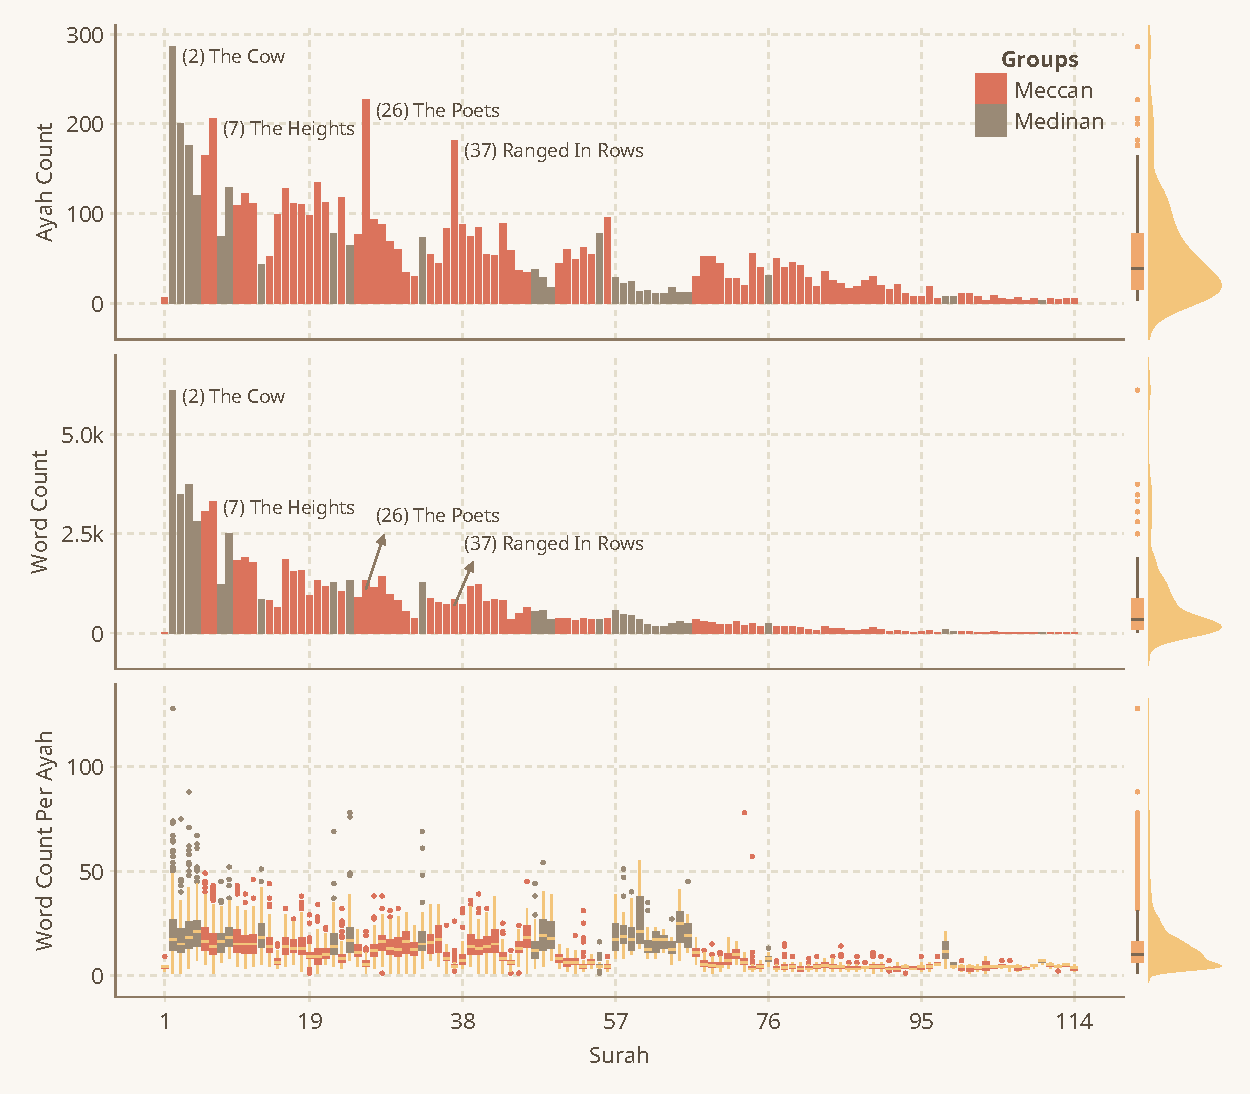
\includegraphics[width=\textwidth]{img/plot1.pdf}
    \caption{Statistics of the words and \arb[trans]{ayAt} \arb{ayAt} (verses) of the Qur'\=an}
    \label{fig:ayah_word_count_with_desc}
\end{figure}

As shown in Figure \ref{fig:ayah_word_count_with_desc}, both the Box and Density plots are tied to each other. This is indeed the case because both are describing the same information but presented in different style of visualization. In fact, Histogram is also used to describe the same information as the Box and Density, and the three are therefore related. So much so, that the three can be put into one graph. As to how to interpret these, readers are referred to for further details \textcolor{red}{[to add reference]}.
\begin{exmp}[Frequency Distribution]\label{ex:frequency_distribution}
Consider again the task of drawing an \arb[trans]{'ayAt} \arb{'ayAt} from the Qur'\=an, suppose the \arb[trans]{'ayAt} \arb{'ayAt} are separated into \arb{makkiyyaT} Meccan and \arb{madaniyyaT} Medinan, what is the probability of getting at most 10 \arb[trans]{kalimAt} \arb{kalimAt} or words in a sampled \arb[trans]{'ayAt} \arb{'ayAt} from \arb{makkiyyaT} Meccan \textit{surah}s \arb{sUr}?\\
\textit{Solution:} To answer this, Figure \ref{fig:meccan_medinan_word_count_per_ayah} shows the \textit{histograms} with the \textit{box plots} and the \textit{rainclouds} plots. The figure shows the frequency of the \arb[trans]{kalimAt} \arb{kalimAt} or words in a sampled \arb[trans]{'ayAt} \arb{'ayAt}. This frequency describes the distribution of the \arb[trans]{kalimAt} \arb{kalimAt}. To interpret this, the Medinan \arb{madaniyyaT} histogram shows that most of the \arb[trans]{'ayAt} \arb{'ayAt} have about 10 to 20 \arb[trans]{kalimAt} \arb{kalimAt} or words in total. This conclusion is based on the where the box of the box plot is located, which also corresponds to the area where the bars of the histogram are high, and also where most of the points or 'droplets' from the rainclouds plot are congested. With that said, \textit{historgram}, \textit{box plot}, and \textit{rainclouds} are related and are telling the same story from different perspectives. It should be noted that, the rainclouds plot is not a common visualization tool. 

Now, comparing the numbers from Medinan \arb{madaniyyaT} to the \arb[trans]{'AyAt 'l-makkiyyaTu} \arb{'AyAt 'l-makkiyyaTu}, there are about 5 to 15 \arb[trans]{kalimAt} \arb{kalimAt} to expect per \arb[trans]{'ayAt} \arb{'ayAt} based on Figure \ref{fig:meccan_medinan_word_count_per_ayah}. 

\begin{figure}[!t]
    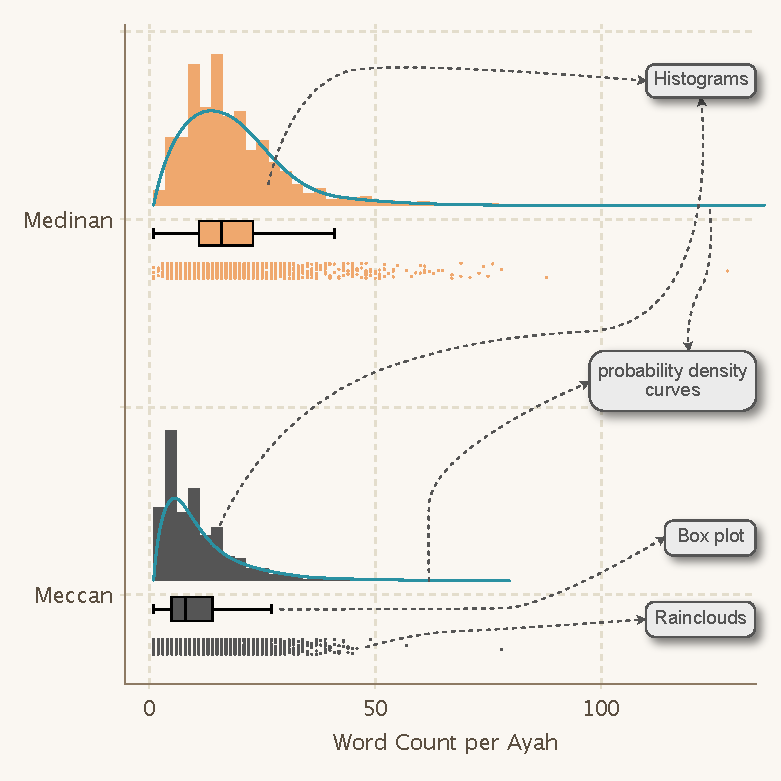
\includegraphics[width=\textwidth]{img/plot3.pdf}
    \caption{Probability density function plot of word count per \arb[trans]{'ayAt} \arb{'ayAt} by revelation location, in relation to its box plot and rainclouds.}
    \label{fig:meccan_medinan_word_count_per_ayah}
\end{figure}

The question has not been answered yet though, the above discussions only explains how to interpret the graphs in Figure \ref{fig:meccan_medinan_word_count_per_ayah}. So to answer the question, one simply needs to total the number of \arb[trans]{'AyAt} \arb{'AyAt} with at most 10 \arb[trans]{kalimAt} \arb{kalimAt} or words and divide this with the total number of \arb[trans]{'AyAt 'l-makkiyyaTu} \arb{'AyAt 'l-makkiyyaTu}. The answer is as follows, and this is part of the result of this paper: there are 4613 \arb[trans]{'AyAt 'l-makkiyyaTu} \arb{'AyAt 'l-makkiyyaTu}, and out of these is 2602 \arb[trans]{'AyAt 'l-makkiyyaTu} \arb{'AyAt 'l-makkiyyaTu} with at most 10 words. Therefore, the probability is $\frac{2602}{4613}=0.612$ or 61.2\% probability. Formally, if $X$ is the random variable of the event of observing at most 10 \arb[trans]{kalimAt} \arb{kalimAt} in a \arb[trans]{'AyAt 'l-makkiyyaTu} \arb{'AyAt 'l-makkiyyaTu}, then 
\begin{align}
     p(X\leq 10)=&\sum_{x=0}^{10} p(X=x)\label{ex_eq:prob_lesseq_10}\\
    =& p(X=0)+ p(X=1)+ p(X=2)+\cdots+ p(X=10)\label{ex_eq:freq_dist_prob1..10}\\
    =&0+\frac{24}{4613}+\frac{172}{4613}+\cdots+\frac{222}{4613}\label{ex_eq:freq_dist_probval1..10}\\
    =&\frac{2602}{4613}=0.612\label{ex_eq:prob_0612}
\end{align}

From Eq. \ref{ex_eq:freq_dist_prob1..10}, $ p(X=0)$ is the probability of observing zero \arb[trans]{kalimaT} \arb{kalimaT} in a \arb[trans]{'AyAt 'l-makkiyyaTu} \arb{'AyAt 'l-makkiyyaTu}, and $ p(X=1)$ is the probability of observing one \arb[trans]{kalimaT} \arb{kalimaT} in a \arb[trans]{'AyAt 'l-makkiyyaTu} \arb{'AyAt 'l-makkiyyaTu}, and so on. The numbers in Eq. \ref{ex_eq:freq_dist_probval1..10} are the number of \arb[trans]{'AyAt 'l-makkiyyaTu} \arb{'AyAt 'l-makkiyyaTu} having zero, one, two, to ten \arb[trans]{kalimAt} \arb{kalimAt}.

\end{exmp}
\section{Population and Sample}
Statistics is a branch of science that is concerned with understanding how the data behave based on a sample---a small set of the said data. It uses statistical methodologies to understand these behavior such as probability mass/density function, and use the findings from these tools on the sampled data as a conclusion for the population---the overall data.

Figure \ref{fig:pop_sample} illustrates the relation of population and sample data. A good example of this is the political surveys on the pulse of the nation on the candidates prior to election. Private entities like PulseAsia\footnote{\url{https://pulseasia.ph/}} and Social Weather Station\footnote{\url{https://www.sws.org.ph/swsmain/home/}} (SWS) do their survey by  sampling from the total population of the Philippines, hence the name survey.

The statistics computed from the surveys like the percentage of votes for particular political candidate are referred as estimates, this is because the computation was done in a sample of the population and not on the population itself. It is therefore important that for these estimates to be accurate representation of the nation's opinion, it has to be representative of the population. That is, the sample shouldn't be bias and leaning to the opinions of the few only and not of the whole nation.

The importance of the sample data as illustrated below follows from the fact that it saves time and cost since interviewing 2500 compared to 100,000 is better compromise for the estimated vote percentages. Further, since these samples requires to well represent the population, the computations of the statistics are estimated using statistical models, like probability mass/density functions, and other models like linear and nonlinears discussed in Section \ref{sec:stat_modeling}. The next example will illustrate the idea population and sample, and how probabilistic modeling can help in understanding insights and answering more questions.
\begin{figure}[t]
    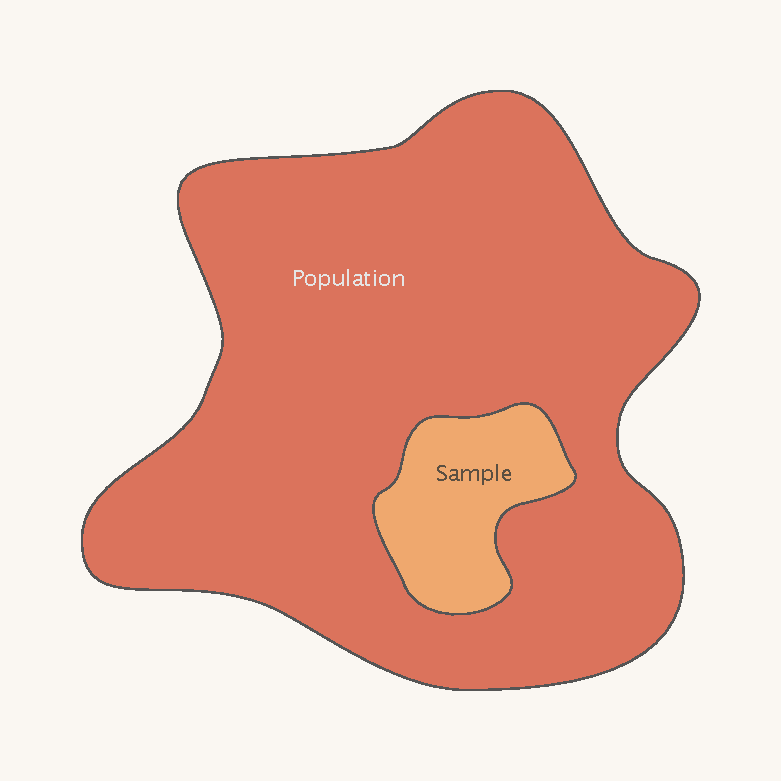
\includegraphics[width=\textwidth]{img/pop_sample.pdf}
    \caption{Population and sample illustration}
    \label{fig:pop_sample}
\end{figure}
\begin{exmp}\label{ex:population_sample_distribution_meccan_words}
Consider the task of sampling 250 \arb[trans]{'AyAt} \arb{'AyAt} from the population of \arb[trans]{'AyAt 'l-makkiyyaT}, describe the statistics of the population and the sample.\\
\textit{Solution:} In Statistics, there are several ways to sample from data, the simplest approach is through the use of \textit{uniform distribution}, that is, the sampling assumes that all data from the population are distributed equally, in the sense that all data points have equal chance of being selected. The other approach is through a \textit{weighted distribution}, where a probability is assigned to each of the data points in the population, so that, the selection will be biased to those with high probability. Figure \ref{fig:meccan_words_sampling} shows the graphs or plots of the population distribution of \arb[trans]{kalimAtu 'l-makkiyyaT} \arb{kalimAtu 'l-makkiyyaT}, which is presented as the top plot, this distribution of \arb{kalimAtu 'l-makkiyyaT} is the same one shown in the bottom plot of Figure \ref{fig:meccan_medinan_word_count_per_ayah}. 

To draw 100 samples from the said population, a simple random sampling without replacement (SRSWOR) is used for selecting or drawing samples. SRSWOR works by randomly selecting sample from the population and then setting it aside as the first sample. The resulting 100 samples are plotted in the bottom plot of Figure \ref{fig:meccan_words_sampling}.

As discussed above, the sample needs to be representative of the population. Figure \ref{fig:meccan_words_sampling} shows that the sampling distribution has more or less the same shape as the population. So that, the statistics are shown in Table \ref{tbl:meccan_words_pop_sample_stats}. From the said table, it can be seen that in terms of centrality, the both data are almost the same, for example the mean is 12.42 for the population and 10.64 for the sample. The reason why the mean in the population is much higher is due to the outlier in the population, which is seen in the extent of the tail of the Kernel Density Estimate in Figure \ref{fig:meccan_words_sampling}. In fact, this is seen in the Median in Table \ref{tbl:meccan_words_pop_sample_stats}, where  the estimate are almost the same. This is because the median is not affected by the outlier. However, the variance did suffer from the outlier in the population, with 50\% reduction in the sample variance, 54.15 to 48.96. The sample will less likely get the outlier as the sample since the outlier is only one observation from the 4163 total Meccan surahs.

The estimates got from the sample ideally are taken from a probabilistic model fitted into the sample data. This computation will be discussed in the next example.

\begin{table}
    \caption{Descriptive statistics of the population and sample data of \arb[trans]{kalimAtu 'l-makkiyyaT} \arb{kalimAtu 'l-makkiyyaT}}
    \label{tbl:meccan_words_pop_sample_stats}
    \begin{tabularx}{\textwidth}[!h]{XXXXl}
        \toprule
        Data&Mean&Median&Variance&Std. Deviation\\
        \midrule
        Population&10.28&8&54.15&7.36\\
        Sample&10.64&9&48.96&7.00\\
        \bottomrule
    \end{tabularx}
\end{table}
\begin{figure}[t]
    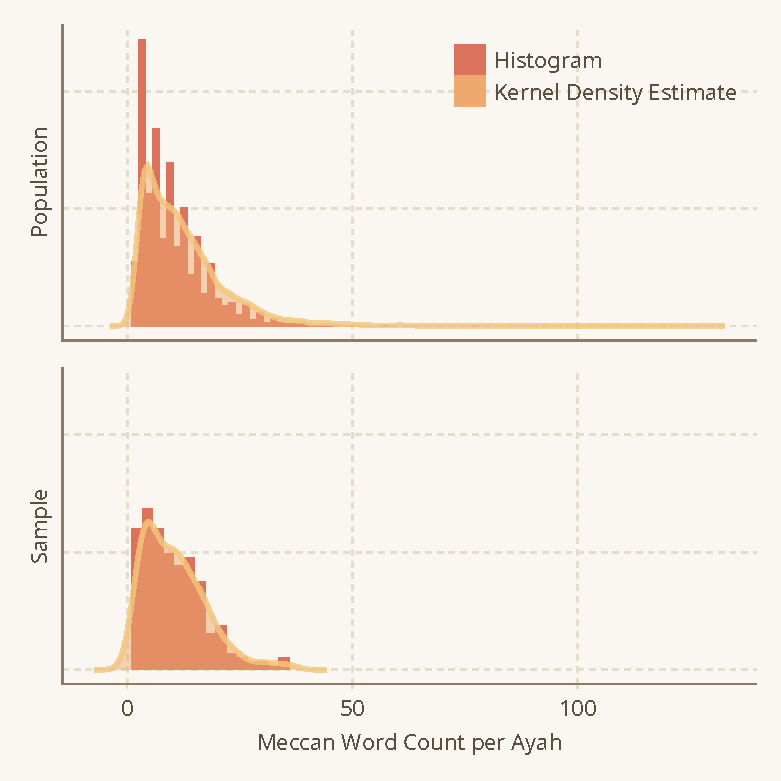
\includegraphics[width=\textwidth]{img/plot5.pdf}
    \caption{Population and sample distribution of Meccan }
    \label{fig:meccan_words_sampling}
\end{figure}

\end{exmp}
\begin{exmp}
Consider again Ex. \ref{ex:population_sample_distribution_meccan_words}, suppose the sample data is the only data available, how will you compute the probability of getting exactly 35 \arb[trans]{kalimAtu 'l-sUratu 'l-makkiyyaTu} \arb{kalimAtu 'l-sUratu 'l-makkiyyaTu}?\\
\textit{Solution:} To answer this question, one might approach this using the frequency distribution as in Ex. \ref{ex:frequency_distribution}. However, the use of frequency distribution from the said example is applicable since that deals with the population data, which is already the true probability, and there is no need to do some estimation. It is like try to get the average height of male Filipinos in the Philippines by doing census across the population, for such case, why would you do an estimate if you have all the census data of all heights of the Filipino, wouldn't it be easier to just do the average computation directly? This is the analogy for the frequency distribution used in Ex. \ref{ex:frequency_distribution}, that is, no need to do some estimation. However, for this problem, the assumption is that only the sample is available, that is, not all of the population is available. With that said, the best solution is to do some estimation. Now, doing an estimation is possible using the samples only, that is, using the idea of frequency distribution but this time applying it on the sample. This is becaus the sample was done using a random sampling, which more or less representative of the population. However, using this approach may possess a problem, let's see what that problem will likely be by forcing the approach in Ex. \ref{ex:frequency_distribution}, following the computation as in Eq. (\ref{ex_eq:prob_lesseq_10}) to Eq. (\ref{ex_eq:prob_0612}). 

Let $X$ again be the random variable of an event of observing 35 \arb[trans]{kalimAt} \arb{kalimAt}, this time from the sample, then
\begin{equation}\label{eq:probx_eq_35}
     p(X=35)=\begin{cases}
        \displaystyle\frac{0}{250}=0,&\text{if sample data}\\
        \displaystyle\frac{5}{4613}=0.0011,&\text{if population data}
    \end{cases}
\end{equation}
From the Eq. \ref{eq:probx_eq_35}, it shows that if we use the sample data for estimating the probability of observing 35 \arb{kalimAt}, then the answer above is 0, meaning by estimate there is a 0 chance of observing a 35 \arb{kalimAt} from a \arb[trans]{'AyAtu 'l-makkiyyaTu} \arb{'l-sUrAtu 'l-makkiyyaTu}. This conclusion is indeed misleading, since according to the population data, there are \arb[trans]{'AyAtu 'l-makkiyyaTu} \arb{'AyAtu 'l-makkiyyaTu} that has 35 \arb[trans]{kalimAt} \arb{kalimAt}. 

So, how to properly estimate this then? This is where the concept of probabilistic modeling comes in. For this problem, the data is count, and that the event of observing 10 \arb[trans]{kalimAtu 'l-sUratu 'l-makkiyyaTu} \arb{kalimAtu 'l-sUratu 'l-makkiyyaTu} in an \arb{'ayaT} is known to be best modeled by a Poisson distribution defined in Defn. \ref{defn:poisson_mass_function}. Ex. \ref{ex:poisson_distribution_sample} will discuss how to solve this. 
\end{exmp}
\section{Probability Distributions}
\begin{defn}[Poisson Mass Function]\label{defn:poisson_mass_function}
Let $X$ be a random variable and let $\lambda>0$ be a parameter, then if $x$ is the random value, then the \textit{Poisson} mass function is given by:
\begin{equation}
     p(X=x)=\frac{\lambda^x\exp(-\lambda)}{x!}
\end{equation}
\end{defn}
\begin{exmp}\label{ex:poisson_distribution_sample}
Consider again Ex. \ref{ex:population_sample_distribution_meccan_words}, the problem can be solved using the Poisson distribution.
\end{exmp}
\begin{defn}[Normal Density Function]
Let $Y$ be a random variable and let $\mu\in\mathbb{R}$ and $\sigma\in\mathbb{R}$ be the mean and variance parameters, if $y$ is the random value, then the \textit{Gaussian} or \textit{Normal} density function is given below:
\begin{equation}
     p(Y=y):=\frac{1}{\sqrt{2\pi\sigma^2}}\exp\left\{-\frac{(y-\mu)^2}{\sigma^2}\right\},\quad\text{where}\;-\infty<y<\infty
\end{equation}
\end{defn}
\begin{defn}[Dirichlet Density Function]
Let $\mathbf{Y}$ be a vector random variable with a random value $\mathbf{y}:=[y_1,\cdots,y_k]^{\text{T}}$ and let $\boldsymbol{\alpha}:=[\alpha_1,\cdots,\alpha_k]^{\text{T}}$ be the parameters, then the \textit{Dirichlet} density function is defined as
\begin{equation}
     p(\mathbf{X}=\mathbf{x};\boldsymbol{\alpha}):=\frac{1}{B(\boldsymbol{\alpha})}\prod_{i=1}^kx_i^{\alpha_i-1},
\end{equation}
where,
\begin{equation}
    B(\boldsymbol{\alpha}):=\frac{\displaystyle\prod_{i=1}^k\Gamma(\alpha_i)}{\Gamma\left(\sum_{i=1}^k\alpha_i\right)}
\end{equation}

\end{defn}
\begin{defn}[Multinomial Mass Function]
Let $\mathbf{X}$ be a vector random variable with a random value $\mathbf{x}:=[x_1,\cdots,x_k]^{\text{T}}$ such that $x_i\geq 0,\forall i \in[1,k]$, let $\boldsymbol{q}:=[q_1,\cdots,q_k]^{\text{T}}$ and $n$ be the parameters, the probability mass function of a Multinomial distribution is 
\begin{align}
    f(x_1,\cdots,x_k;n,q_1,\cdots,q_k):=& q(X_1=x_1\;\text{and}\;\cdots\;\text{and}\;X_k=x_k)\nonumber\\
    =&\begin{cases}
        \displaystyle\frac{n!}{x_1!\cdots x_k!}q_1^{x_1}\times\cdots\times q_k^{x_k},&\text{when}\;\sum_{i=1}^kx_i=n\\
        0&\text{otherwise},
    \end{cases}
\end{align}
\end{defn}

\section{Frequentist Estimation}\label{sec:stat_modeling}
Probability distributions are fundamental models that can be used to describe some characteristics of the data. However, combinations of variables, and accounting dynamics of the observations can lead into other types of models as well. In general, a statistical model can be written using the following formula:
\begin{equation}
    y=f(x|\mathbf{\Theta})+\varepsilon,
\end{equation}
where $y\sim p(\cdot)$ and $\varepsilon\sim p(\cdot)$.

There are two main ways to estimating the parameters $\boldsymbol{\Theta}$, and that is either through Frequentist or Bayesian approach.
\subsection{Maximum Likelihood Estimation}
Maximum likelihood estimation (MLE) is a fundamental concept in statistics that provides a method for estimating the parameters of a statistical model based on the observed data. The basic idea behind MLE is to find the parameter values that make the observed data most likely or probable under the assumed statistical model. The concept of MLE can be explained as follows:

Suppose we have a random sample of observations $X := \{x_1, x_2, ..., x_n\}$ from a probability distribution $f(x | \theta)$, where $\theta$ represents the unknown parameter(s) of the distribution. The likelihood function, denoted as $\mathcal{L}(\theta | X)$, is the joint probability density (or probability mass function for discrete distributions) of the observed data $X$, treated as a function of the parameter(s) $\theta$.
\begin{equation}
    \mathcal{L}(\theta | X) = f(x_1 | \theta) \times f(x_2 | \theta) \times\cdots\times f(x_n | \theta)    
\end{equation}

The maximum likelihood estimate (MLE) of $\theta$, denoted as $\hat{\theta}$, is the value of $\theta$ that maximizes the likelihood function $\mathcal{L}(\theta | X)$. In other words, $\hat{\theta}$ is the value of θ that makes the observed data most likely or probable under the assumed statistical model.
\begin{equation}
    \hat{\theta} = \underset{\theta}{\arg\max} \mathcal{L}(\theta | X)    
\end{equation}

In practice, it is often easier to work with the log-likelihood function, denoted as $\ell(\theta | X) = \log(\mathcal{L}(\theta | X))$, since the logarithm is a monotonic function and maximizing the log-likelihood is equivalent to maximizing the likelihood.
\begin{equation}
   \hat{\theta} = \underset{\theta}{\arg\max}\ell(\theta | X)    
\end{equation}
\begin{exmp}[Normal distribution]
    Suppose we have a random sample $X = \{x_1, x_2,\cdots, x_n\}$ from a normal distribution with unknown mean μ and known variance $\sigma^2$. The likelihood function is:
    \begin{equation}
        \mathcal{L}(\mu | X) = \frac{1}{(\sqrt{2\pi\sigma^2})^n}\exp\left(-\sum_{\forall i}(x_i - \mu)^2 / (2\sigma^2)\right)
    \end{equation}
    
    Taking the log and differentiating with respect to $\mu$, setting the derivative equal to zero, and solving for $\mu$, we get the maximum likelihood estimate or MLE of $\mu$:
    \begin{equation}
        \hat{\mu} = \frac{1}{n}\sum_{\forall i}x_i
    \end{equation}
\end{exmp}
MLE has several desirable properties, such as consistency (the MLE converges to the true parameter value as the sample size increases) and asymptotic normality (the sampling distribution of the MLE approaches a normal distribution as the sample size increases), which make it a widely used method in statistical inference and modeling.
\subsection{Numerical Approximation}
There are several ways to numerically estimate the parameters of the model using mathematical programming. The popular algorithm that is very common in Machine Learning is the \textit{gradient descent} (GD) given in Algorithm \ref{algo:GD}. Suppose $\nabla\ein(\hat{\mathbf{w}}^{(r)})$ is the gradient of the cost function at the $r$th iteration. $\ein$ is defined as \mbox{the \textit{in-sample error}} or the error in the training dataset, $\gamma$ is the \textit{learning-rate} parameter of the algorithm and $\nu$ is the \textit{precision} parameter. As an illustration, consider Example \ref{ex:gd}.\vspace{.4cm}

\begin{algorithm}
\caption{\it Gradient Descent}
\label{algo:GD}
\begin{algorithmic}[1]\vspace{.2cm}
\item Initialize $\hat{\mathbf{w}}^{(r)},r=0$\vspace{.2cm}
\While{$\lVert \hat{\mathbf{w}}^{(r+1)}-\hat{\mathbf{w}}^{(r)}\rVert > \nu$}\vspace{.2cm}
\State $\hat{\mathbf{w}}^{(r+1)}\triangleq \hat{\mathbf{w}}^{(r)} - \gamma\nabla\ein(\hat{\mathbf{w}}^{(r)})$\vspace{.2cm}
\State $r\triangleq r + 1$\vspace{.2cm}
\EndWhile\\\vspace{.2cm}
\Return $\hat{\mathbf{w}}^{(r)}$ and $r$.
\end{algorithmic}
\end{algorithm}
\vspace{-.3cm}

\begin{exmp}\label{ex:gd}
Suppose the loss function is given by
\begin{equation}\label{eq:errgd1}
\ein(w)\triangleq w^4 - 3w^3 + 2.
\end{equation}
The first derivative of the above equation with respect to $w$ is given by ${\ein'(w)=4w^3-9w^2}$. Let the initial guess be $\hat{w}^{(0)}=.1$ and let $\gamma=.01$ with $\nu=.00001$. Then $\nabla\ein(\hat{w}^{(0)})=\ein'(\hat{w}^{(0)})=-0.086$, so that $\hat{w}^{(1)}\triangleq\hat{w}^{(0)}-.01(-0.086)=0.10086$, and $|\hat{w}^{(1)} - \hat{w}^{(0)}| = 0.00086> \nu$. It turns out that 173 iterations are needed to satisfy \mbox{the inequality}, $|\hat{w}^{(r+1)} - \hat{w}^{(r)}| \ngtr \nu$.
\end{exmp}
In practice, however, there are hundreds to millions of data points that need to be summarized, so that at each iteration, the parameters are updated \textit{after} \mbox{the presentation} of \textit{all} the training examples that constitute an \textit{epoch} --- one complete presentation of the entire training dataset during the learning process \cite{Haykin1998}. In this setting, GD is sometimes called \textit{batch gradient descent} (BGD).
\subsection{Stochastic Gradient Descent}\label{sec:sgd}
An alternative to BGD is SGD or \textit{stochastic gradient descent}. SGD updates the parameter using only one observation for every iteration, which is a lot faster. Further, BGD is prone to local minimum since GD does so. This is guaranteed for misspecified initial value especially for high dimensional nonlinear error surface function. \mbox{The stochasticity} of the SGD follows from the randomization of the dataset at each epoch, and contrary to BGD, the SGD is not expected to converge to \mbox{the global} minimum, instead it will only stay around the global solution (\textit{see} Algorithm \ref{algo:SGD}). Example \ref{exmp:bgdslr} illustrates the application of mathematical programming in estimating the parameters of a simple linear regression model.
\vspace{.4cm}

\begin{algorithm}[!h]
\caption{\it Stochastic Gradient Descent}
\label{algo:SGD}
\begin{algorithmic}[1]\vspace{.2cm}
\item Initialize $\hat{\mathbf{w}}^{(r)},r=0$\vspace{.2cm}
\While{$\lVert \hat{\mathbf{w}}^{(r)}-\hat{\mathbf{w}}^{(r+1)}\rVert > \nu$}\vspace{.2cm}
\State Randomize the data set ($\mathbf{x}_i,\mathbf{y}_i$) with respect to $i$.\vspace{.2cm}
\For{$i \in\{1,\cdots, n\}$}\vspace{.2cm}
\State Update the parameters
\begin{align}\nonumber
\hat{\mathbf{w}}^{(r)}&\triangleq \hat{\mathbf{w}}^{(r)} - \gamma\nabla\mathrm{e}(h(\mathbf{x}_i,\hat{\mathbf{w}}^{(r)}),\mathbf{y}_i)\\\nonumber
&=\hat{\mathbf{w}}^{(r)} - \gamma\frac{\partial}{\partial\mathbf{w}}\left\{\frac{1}{2}[h(\mathbf{x}_i,\hat{\mathbf{w}}^{(r)})-\mathbf{y}_i]^2\right\}
\end{align}
%\State Compute $\mathrm{e}^{(r)}\triangleq\mathrm{e}(h(\mathbf{x}_k,\hat{\mathbf{w}}^{(r+1)}),\mathbf{y}_k)$\vspace{.2cm}
\EndFor\vspace{.2cm}
\State $\hat{\mathbf{w}}^{(r+1)}\triangleq \hat{\mathbf{w}}^{(r)}$\vspace{.2cm}
%\State Compute the cost function
%\begin{equation}
%\ein(h)=\frac{1}{n}\sum_{i=1}^K\mathrm{e}(h(\mathbf{x}_i,\hat{\mathbf{w}}^{(r+1)}),\mathbf{y}_i)
%\end{equation}
\EndWhile\vspace{.2cm}
\item\Return $\hat{\mathbf{w}}^{r}$ and $r$.
\end{algorithmic}
\end{algorithm}
\section{Bayesian Estimation}
Bayesian estimation is a statistical approach that incorporates prior knowledge or beliefs about the parameters of interest into the estimation process. It combines the prior knowledge with the observed data to obtain updated beliefs or estimates of the parameters, known as the posterior distribution.
The Bayesian estimation framework is based on Bayes' theorem, which relates the conditional probabilities of events. In the context of parameter estimation, Bayes' theorem can be expressed as:
\begin{equation}
    p(\theta | X) = \frac{p(X | \theta)p(\theta))}{p(X)}
\end{equation}
where $p(\theta | X)$ is the posterior distribution, representing the updated beliefs about the parameter(s) $\theta$ after observing the data X. $p(X | \theta)$ is the likelihood function, which quantifies the probability of observing the data X given the parameter(s) $\theta$. $p(\theta)$ is the prior distribution, representing the initial beliefs or knowledge about the parameter(s) $\theta$ before observing the data. $p(X)$ is the marginal likelihood or the probability of observing the data X, which acts as a normalizing constant.
\subsection{Laplace's Approximation}\label{sec:laplace}
The simplest approximation to the posterior distribution of the parameter of interest is the Laplace's approximation. The idea behind this procedure is to use a Gaussian approximator, $\g(x)$, such that it is centered on the mode of the target distribution, $ p(x)$. To illustrate, suppose
\begin{equation}
 p(x):=\frac{f(x)}{Z},\quad\mathrm{where}\;Z:=\int f(x)\D x.
\end{equation}
Using basic calculus, the mode\footnote{obtained using maximum \textit{a posteriori} (MAP)} of the posterior distribution, say at $x=x_{\text{MAP}}$, is achieved by taking the derivative of the objective function with respect to the $x$-axis, such that the gradient of the function is $0$ at $x=x_{\text{MAP}}$. That is,
\begin{equation}
\frac{\D f(x)}{\D x}\bigg|_{x=x_{\text{MAP}}}=0.
\end{equation}
The Gaussian distribution has the property that its logarithm is a quadratic function of the variables \cite{bishop}. Hence, the following is an approximation of \mbox{the log} of \mbox{the objective} function using second-order Taylor series expansion centered on \mbox{the mode} $x_{\text{MAP}}$, 
\begin{align}
\log f(x)=&\log f(x_{\text{MAP}})+\frac{\D \log f(x)}{\D x}\bigg|_{x=x_{\text{MAP}}}(x-x_{\text{MAP}})\\
&+\frac{\D^2 \log f(x)}{\D x^2}\bigg|_{x=x_{\text{MAP}}}\frac{(x-x_{\text{MAP}})^2}{2}+\mathcal{O}(x)\\
\approx&\log f(x_{\text{MAP}})+\frac{\D^2 \log f(x)}{\D x^2}\bigg|_{x=x_{\text{MAP}}}\frac{(x-x_{\text{MAP}})^2}{2}.
\end{align}
Exponentiating both sides of the above equations becomes
\begin{equation}
f(x)\approx f(x_{\text{MAP}})\exp\left[\frac{\D^2 \log f(x)}{\D x^2}\bigg|_{x=x_{\text{MAP}}}\frac{(x-x_{\text{MAP}})^2}{2}\right],
\end{equation}
so that the normalized estimator $\g(x)$ is given by
\begin{equation}
\g(x)=\left(-\frac{1}{2\pi}\frac{\D^2 \log f(x)}{\D x^2}\bigg|_{x=x_{\text{MAP}}}\right)^{1/2}\exp\left[\frac{\D^2 \log f(x)}{\D x^2}\bigg|_{x=x_{\text{MAP}}}\frac{(x-x_{\text{MAP}})^2}{2}\right].
\end{equation}
\vspace{-1cm}
\begin{exmp}
Suppose the posterior distribution is a chi-square of the form: $p(x):=\frac{x^{k-1}\exp\left(-\frac{x^2}{2}\right)}{Z}$, with $k$ degrees of freedom where $Z:=2^{\frac{k}{2}-1}\Gamma\left(\frac{k}{2}\right),\quad x>0$. Using Laplace, \mbox{the approximator} to the posterior distribution is obtained as follows:\\[.3cm]
The log-likelihood of the density function is given by
\begin{equation}
\ell(x):=\log p(x)=(k-1)\log x-\frac{x^2}{2}+\mathcal{C},
\end{equation}
where $\mathcal{C}$ is the constant. The mode of this posterior is given by
\begin{align}
\frac{\partial}{\partial x}\log  p(x)&=\frac{k-1}{x_{\text{MAP}}}-x_{\text{MAP}}\overset{\text{set}}{=}0\\
x_{\text{MAP}}&=\sqrt{k-1}.
\end{align}
The second partial derivative of the log-likelihood with respect to $x$ evaluated at $x_{\text{MAP}}$ is
\begin{equation}\label{eq:laplaceexapprox}
-\frac{\partial^2}{\partial x^2}\log  p(x)\bigg|_{x=x_{\text{MAP}}}=1-\frac{1-k}{x_{\text{MAP}}^2}=2.
\end{equation}
Thus the estimate of the posterior is given by a Gaussian distribution with mean $\mu=\sqrt{k-1}$ and variance $\sigma^2 = \frac{1}{2}$. Figure \ref{fig:laplaceapprox} visualizes the Gaussian distribution as an approximator to the posterior distribution.
\end{exmp}
Now consider the case where $\mathbf{x}\in\mathbb{R}^{d}$, such that $ p(\mathbf{x}):=\frac{f(\mathbf{x})}{Z}$. Analogous to \mbox{the univariate} case, the Laplace's approximation for $ p(\mathbf{x})$ is obtained by aligning \mbox{the mean} of the multivariate Gaussian distribution to the mode of the posterior density, denoted by $\mathbf{x}_{\text{MAP}}$. As before, the log-likelihood of $f(\mathbf{z})$ is given by \mbox{the following} equation
\begin{equation}\label{eq:laplacemultivar}
\log f(\mathbf{x})\approx\log f(\mathbf{x}_{\text{MAP}})-\frac{1}{2}(\mathbf{x}-\mathbf{x}_{\text{MAP}})^{\text{T}}\boldsymbol{\mathfrak{H}}(\mathbf{x}-\mathbf{x}_{\text{MAP}}),
\end{equation}
where $\boldsymbol{\mathfrak{H}}$ is the Hessian matrix defined by
\begin{equation}\label{eq:2ndderivlaplace}
\boldsymbol{\mathfrak{H}}:=-\frac{\partial^2}{\partial\mathbf{x}^2}\log f(\mathbf{x})\bigg|_{\mathbf{x}=\mathbf{x}_{\text{MAP}}}.
\end{equation}
Exponentiating Equation (\ref{eq:laplacemultivar}) leads to the normalized approximator, $\g(\mathbf{x})=\mathcal{N}_d(\mathbf{x}|\mathbf{x}_{\text{MAP}},\boldsymbol{\mathfrak{H}}^{-1})$.
\subsection{Markov Chain Monte Carlo (MCMC)}
Laplace has the advantage of being simple and easy to use. However, like any approximator, it has limitations especially on multimodal densities since it uses Gaussian as estimate to the posterior distribution. Most interesting high dimensional Bayesian models have multimodal \textit{a posteriori}, which can't be captured through Laplace's method. To address this problem, sampling methods are instead used for approximating the \textit{a posteriori}. These family of sampling methods are called Markov Chain Monte Carlos (MCMC) with \textit{Metropolis-Hasting} (MH) and \textit{Gibbs sampling} as \mbox{the popular} MCMCs. Further, for sophisticated MCMCs, the algorithms available are not limited to \textit{Hamiltonian Monte Carlo} (HMC) and \textit{Stochastic Gradient HMC}.
\subsection{Metropolis-Hasting}\label{sec:metropolishasting}
The idea of the MH algorithm is to randomly walk in the support of the target density such that the random step is governed by the proposal distribution $\g(\cdot)$. \mbox{The assumption} is that the posterior distribution has no closed-form solution, but the kernel, which is the unnormalized form of the target density is easy to evaluate. This is the advantage of the Metropolis-Hasting algorithm where the \textit{a posteriori} is not necessarily be normalized --- often the difficulty in simplifying the model evidence of the Bayes' rule. Let $ p(\cdot)$ be the \textit{a posteriori}, then the Metropolis-Hasting algorithm is given in Algorithm \ref{algo:mcmcmh}.
\vspace{.4cm}

\begin{algorithm}[!t]
\caption{\it Metropolis-Hasting MCMC}
\label{algo:mcmcmh}
\begin{algorithmic}[1]\vspace{.2cm}
\item Initialize $\mathbf{w}_{r}\sim\g(\mathbf{w}),r=0$\vspace{.2cm}
\For {$r\in\{1,\cdots, r_{\text{max}}\}$}\vspace{.2cm}
\State Propose: $\mathbf{w}_{new}\sim\g(\mathbf{w}_{new}|\mathbf{w}_{r-1})$\vspace{.2cm}
\State Acceptance: $\alpha(\mathbf{w}_{new}|\mathbf{w}_{r-1}):=\min\left\{1,\frac{ p(\mathbf{w}_{new}|\mathbf{w}_{r-1})\g(\mathbf{w}_{r-1}|\mathbf{w}_{new})}{ p(\mathbf{w}_{r-1}|\mathbf{w}_{new})\g(\mathbf{w}_{new}|\mathbf{w}_{r-1})}\right\}$\vspace{.2cm}
\State Draw $x\sim\text{Unif}(0,1)$\vspace{.2cm}
\If {$x<\alpha(\mathbf{w}_{new}|\mathbf{w}_{r-1})$}\vspace{.2cm}
\State $\mathbf{w}_{r}:=\mathbf{w}_{new}$
\vspace{.2cm}
\Else \vspace{.2cm}
\State $\mathbf{w}_{r}:=\mathbf{w}_{r-1}$\vspace{.2cm}
\EndIf\vspace{.2cm}
\EndFor
\end{algorithmic}
\end{algorithm}
\vspace{-.3cm}
\begin{exmp}\label{exmp:mcmcmh}
Consider the bivariate Gaussian distribution defined below:
\begin{equation}
f(\mathbf{x}|\boldsymbol{\mu},\boldsymbol{\Sigma})
:=\frac{1}{\sqrt{(2\pi)^d|\boldsymbol{\Sigma}|}}\exp\left[-\frac{1}{2}(\mathbf{x} - \boldsymbol{\mu})^{\text{T}}\boldsymbol{\Sigma}^{-1}(\mathbf{x}-\boldsymbol{\mu})\right].
\end{equation}
Suppose it has the following parameters: 
\begin{equation}\nonumber
\boldsymbol{\mu}:=[10\;-10]^{\text{T}} \quad\text{and}\quad \boldsymbol{\Sigma}:=\left[\begin{array}{cc}1.5^2&\rho(1.5)(1.35)\\\rho(1.5)(1.35)&1.35^2\end{array}\right]
\end{equation}
where ${\rho := .5}$; in order to draw samples from this model, let the proposal distribution defined to be the current step of the random walk plus an increment from a uniform distribution with parameters min = -5 and max = 5.

The random samples drawn by MH are not independent, this is due to \mbox{the design} of the algorithm where the distribution of the candidate sample depends solely on the current sample\footnote{this is the property of the Markov Chain, hence the name MCMC.}. To address this problem, diagnostics are applied using methods such as \textit{thinning}, where every $i$th sample is taken and the rest are discarded; or using \textit{burn-in} where first $n^{\star}$ samples are discarded.

\end{exmp}
\subsection{Gibbs Sampling}\label{sec:gibbssampling}
MH is by far one of the easiest MCMC algorithm for drawing samples from \textit{a posteriori} where direct sampling is not possible. It uses proposal distribution as drivers of the random walk in the support of the target density, which for high dimensional data, the choice of appropriate proposal function is sometimes difficult to specify. As an alternative, Gibbs sampler can be used for taking samples from the posterior distribution. The only requirement is that the joint distribution of the parameters (the \textit{a posteriori}) can be decomposed into conditional distributions of each variable conditioned on other variables. Mathematically, suppose \mbox{the multivariate} distribution is given by $f(\mathbf{w}|\mathscr{D})$, where $\mathbf{w}:=[w_1\;w_2\cdots w_K]^{\text{T}}$, then the Gibbs sampling algorithm is given in Algorithm \ref{algo:mcmcgibbs}.
\vspace{.4cm}

\begin{algorithm}[!b]
\caption{\it Gibbs Sampling MCMC}
\label{algo:mcmcgibbs}
\begin{algorithmic}[1]\vspace{.2cm}
\item Initialize $\mathbf{w}_{r}, r=0$\vspace{.2cm}
\For {$r\in\{1,\cdots, r_{\text{max}}\}$}\vspace{.2cm}
\State $w_1^{(new)}\sim f(w_1|w_2,\cdots,w_K)$\vspace{.2cm}
\State $w_2^{(new)}\sim f(w_2|w_1^{(new)},\cdots,w_K)$\vspace{.2cm}
\State $w_3^{(new)}\sim f(w_3|w_1^{(new)},w_2^{(new)},\cdots,w_K)$\vspace{.2cm}
\State $\vdots\qquad\qquad\qquad\vdots\qquad\qquad\qquad\vdots$\vspace{.2cm}
\State $w_K^{(new)}\sim f(w_K|w_1^{(new)},w_2^{(new)},\cdots,w_{K-1}^{(new)})$\vspace{.2cm}
\State $\mathbf{w}_r:=[w_1^{(new)},\cdots,w_K^{(new)}]^{\text{T}}$\vspace{.2cm}
\EndFor
\end{algorithmic}
\end{algorithm}
\vspace{-.3cm}
\begin{exmp}\label{exmp:gibbs}
Using the same posterior distribution as in Example \ref{exmp:mcmcmh}, the conditional distributions of the parameters conditioned on other parameters are also Gaussian with mean $\mu:=\mu_1 + \left(\frac{\sigma_1}{\sigma_2}\right)\rho(x - \mu_2)$ and standard deviation $\sigma:=\sqrt{(1 - \rho^2)\sigma_1^2}$. Analogous to MH, samples obtained using Gibbs are not independent but with lower autocorrelation compared to the former. As before, the same diagnostics can be done. 
\end{exmp}
\subsection{Bayesian Linear Regression}\label{sec:blr}
As an illustration of Bayesian inference to basic modeling, this section attempts to discuss the Bayesian approach to linear regression. Let ${\mathscr{D}=\{(\mathbf{x}_1,y_1),\cdots, (\mathbf{x}_n,y_n)\}}$ where $\mathbf{x}_i\in\mathbb{R}^{d}, y_i\in \mathbb{R}$ be the pairwised dataset. Suppose the response values, $y_1,\cdots,y_n$, are independent given the parameter $\mathbf{w}$, and is distributed as $y_i\sim\mathcal{N}(\mathbf{w}^{\text{T}}\mathbf{x}_i,\alpha^{-1})$, where $\alpha^{-1}$ is referred to as the \textit{precision} parameter --- useful for later derivation. In Bayesian perspective, the weights are assumed to be random and are governed by some \textit{a priori} distribution. The choice of this distribution is subjective, but choosing arbitrary \textit{a priori} can sometimes or often result to an intractable integration, especially for interesting models. For simplicity, a conjugate prior is used for the latent weights. Specifically, assume that ${\mathbf{w}\sim\mathcal{N}(\mathbf{0},\beta^{-1}\mathbf{I})}$ such that $\beta>0$ is the hyperparameter supposed in this experiment as known value. The posterior distribution based on the Bayes' rule is given by
\begin{equation}\label{eq:bayesrulepost}
	p(\mathbf{w}|\mathbf{y})=\frac{p(\mathbf{w})p(\mathbf{y}|\mathbf{w})}{p(\mathbf{y})},
\end{equation}
where $p(\mathbf{w})$ is the \textit{a priori} distribution of the parameter, $p(\mathbf{y}|\mathbf{w})$ is the likelihood, and $p(\mathbf{y})$ is the normalizing factor. The likelihood is given by
\begin{align}
    p(\mathbf{y}|\mathbf{w})&=\prod_{i=1}^{n}\frac{1}{\sqrt{2\pi\alpha^{-1}}}\exp\left[-\frac{\alpha(y_i-\mathbf{w}^{\text{T}}\mathbf{x}_i)^2}{2}\right]\\
    &=\left(\frac{\alpha}{2\pi}\right)^{n/2}\exp\left[-\sum_{i=1}^n\frac{\alpha(y_i-\mathbf{w}^{\text{T}}\mathbf{x}_i)^2}{2}\right].\label{eq:likelihood:blreg}
\end{align}
In matrix form, this can be written as
\begin{equation}
    p(\mathbf{y}|\mathbf{w})\propto\exp\left[-\frac{\alpha}{2}(\mathbf{y}-\boldsymbol{\mathfrak{A}}\mathbf{w})^{\text{T}}(\mathbf{y}-\boldsymbol{\mathfrak{A}}\mathbf{w})\right]
\end{equation}
where $\boldsymbol{\mathfrak{A}}=\left[(\mathbf{x}_i^{\text{T}})\right]$, i.e. $\boldsymbol{\mathfrak{A}}\in(\mathbb{R}^{n}\times\mathbb{R}^d)$, this matrix is known as the \textit{design matrix}. Given that $\mathbf{w}$ has the following prior distribution
\begin{equation}\label{eq:wpriori}
    p(\mathbf{w})=\frac{1}{\sqrt{(2\pi)^{d}|\beta^{-1}\mathbf{I}|}}\exp\left[-\frac{1}{2}\mathbf{w}^{\text{T}}\beta\mathbf{I}\mathbf{w}\right],
\end{equation}
implies that the posterior has the following form:
\begin{align}
    p(\mathbf{w}|\mathbf{y})&\propto\exp\left[-\frac{\alpha}{2}(\mathbf{y}-\boldsymbol{\mathfrak{A}}\mathbf{w})^{\text{T}}(\mathbf{y}-\boldsymbol{\mathfrak{A}}\mathbf{w})\right]\exp\left[-\frac{1}{2}\mathbf{w}^{\text{T}}\beta\mathbf{I}\mathbf{w}\right]\\
&=\exp\left\{-\frac{1}{2}\left[\alpha(\mathbf{y}-\boldsymbol{\mathfrak{A}}\mathbf{w})^{\text{T}}(\mathbf{y}-\boldsymbol{\mathfrak{A}}\mathbf{w})+\mathbf{w}^{\text{T}}\beta\mathbf{I}\mathbf{w}\right]\right\}.
\end{align}
Expanding the terms in the exponent, becomes
\begin{equation}\label{eq:expterms}
    \alpha\mathbf{y}^{\text{T}}\mathbf{y}-2\alpha\mathbf{w}^{\text{T}}\boldsymbol{\mathfrak{A}}^{\text{T}}\mathbf{y}+\mathbf{w}^{\text{T}}(\alpha\boldsymbol{\mathfrak{A}}^{\text{T}}\boldsymbol{\mathfrak{A}}+\beta\mathbf{I})\mathbf{w}.
\end{equation}
The next step is to complete the square of the above equation such that it resembles the inner terms of the exponential factor of the Gaussian distribution. The quadratic form of the exponential term of a $\mathcal{N}(\mathbf{w}|\boldsymbol{\mu},\boldsymbol{\Sigma}^{-1})$ is given by
\begin{align}
    (\mathbf{w}-\boldsymbol{\mu})^{\text{T}}\boldsymbol{\Sigma}^{-1}(\mathbf{w}-\boldsymbol{\mu})&=(\mathbf{w}-\boldsymbol{\mu})^{\text{T}}(\boldsymbol{\Sigma}^{-1}\mathbf{w}-\boldsymbol{\Sigma}^{-1}\boldsymbol{\mu})\\
&=\mathbf{w}^{\text{T}}\boldsymbol{\Sigma}^{-1}\mathbf{w}-
2\mathbf{w}^{\text{T}}\boldsymbol{\Sigma}^{-1}\boldsymbol{\mu}+\boldsymbol{\mu}^{\text{T}}\boldsymbol{\Sigma}^{-1}\boldsymbol{\mu}.\label{eq:expnorm}
\end{align}
The terms in Equation (\ref{eq:expterms}) are matched up with that in (\ref{eq:expnorm}), so that
\begin{equation}\label{eq:sigmablrgauss}
    \boldsymbol{\Sigma}^{-1}=\alpha\boldsymbol{\mathfrak{A}}^{\text{T}}\boldsymbol{\mathfrak{A}}+\beta\mathbf{I}
\end{equation}
and
\begin{align}
    \mathbf{w}^{\text{T}}\boldsymbol{\Sigma}^{-1}\boldsymbol{\mu}&=\alpha\mathbf{w}^{\text{T}}\boldsymbol{\mathfrak{A}}^{\text{T}}\mathbf{y}\\
    \boldsymbol{\Sigma}^{-1}\boldsymbol{\mu}&=\alpha\boldsymbol{\mathfrak{A}}^{\text{T}}\mathbf{y}\\
    \boldsymbol{\mu}&=\alpha\boldsymbol{\Sigma}\boldsymbol{\mathfrak{A}}^{\text{T}}\mathbf{y}.\label{eq:mublrgauss}
\end{align}
Thus the \textit{a posteriori} is a Gaussian distribution with location parameter in \mbox{Equation (\ref{eq:mublrgauss})} and scale parameter given by the inverse of Equation (\ref{eq:sigmablrgauss}).
\section{Types of Statistical Methods}
\textit{Parametric} and \textit{non-parametric} statistics are two broad categories of statistical methods, each with its own assumptions and applications. The primary difference between them lies in the underlying assumptions made about the population distribution.
\subsection{Parametric}
Parametric statistics are based on the assumption that the data follows a specific probability distribution, such as the normal distribution (also known as the Gaussian distribution). These methods rely on the estimation of parameters (such as the mean and standard deviation) from the sample data to make inferences about the population.
\begin{enumerate}
    \item \textbf{Student's t-test} - for comparing means
    \item \textbf{Analysis of Variance (ANOVA)} - for comparing means across multiple groups
    \item \textbf{Pearson's correlation coefficient} - for measuring linear correlation
    \item \textbf{Linear regression} - for modeling relationships between variables
\end{enumerate}
\subsection{Nonparametric}
Non-parametric statistics, also known as distribution-free tests, do not make assumptions about the underlying probability distribution of the data. These methods are based on the ranks or signs of the data rather than the actual values.
\begin{enumerate}
    \item \textbf{Mann-Whitney U test} - for comparing two independent groups
    \item \textbf{Wilcoxon signed-rank test} - for comparing two related groups or paired samples
    \item \textbf{Kruskal-Wallis test} - for comparing more than two independent groups
    \item \textbf{Spearman's rank correlation coefficient} - for measuring monotonic relationships between variables
\end{enumerate}
\section{Types of Models}
Generally, there are two types of models, the \textit{supervised} and \textit{unsupervised}. The other one that is not common, is the \textit{semi-supervised}. The following sections will elaborate more.
\subsection{Supervised}
Supervised learning models are trained using labeled data, which means that each training example is paired with an output label. The goal is to learn a mapping from inputs to outputs based on the labeled training data, so the model can predict the output for new, unseen inputs. The following are examples of supervised learning models:
\begin{enumerate}
    \item \textbf{Linear Regression} - used for predicting continuous outcomes that are not time dependent.
    \item \textbf{Logistic Regression} - used for binary classification.
    \item \textbf{Neural Networks} - the core model powering most of the big AI models and applications.
\end{enumerate}
\subsection{Unsupervised}\label{sec:unsupervised_models}
Unsupervised learning models are trained using unlabeled data, which means that the data does not have output labels. The goal is to uncover the underlying structure of the data, such as grouping similar data points together or reducing the dimensionality of the data. The following are examples of unsupervised models:

\begin{enumerate}
    \item \textbf{Hierarchical Clustering} - used for finding groups or clusters from the data.
    \item \textbf{Kernel Density Estimation (KDE)} - used for estimating the probability density function of the data.
    \item \textbf{Gaussian Processes} - used for regression and probabilistic classification, modeling distributions over functions.
\end{enumerate}

\chapter{Methodology}
This chapter is organized as follows: Section \ref{sec:topic_modeling_method} will discuss the concept of Topic Modeling, Section \ref{sec:llm_method} will discuss the concept of Large Language Models, and finally Section \ref{sec:code_setup} will discuss how to implement this in Julia programming language.
\section{Topic Modeling}\label{sec:topic_modeling_method}
As presented in Chapter \ref{ch:introduction}, the first objective is to extract the thematic themes of \textit{s\=urahs} \arb{sUr} with at least 1000 words. In Statistics and Machine Learning, this task is called Topic Modeling. There are several ways to do this, but the popular methodology is to use the Latent Dirichlet Allocation (LDA) discussed in the next section.
\subsection{Latent Dirichlet Allocation}\label{sec:lda}
Latent Dirichlet Allocation (LDA) is a Statistical methodology that is based on Bayesian inference \cite{bayes,laplace1986}. It is a generative probabilisitic model for collection of discrete data such as text corpora \cite{blei2003latent}. The main formula is defined below:
\begin{defnx}[Latent Dirichlet Allocation]
Let $\mathbf{W},\mathbf{Z},\boldsymbol{\theta},\boldsymbol{\varphi}$ be the random variables, and let $\alpha$ and $\beta$ be the hyper-parameters, then the probability of generating a document is
\begin{equation}
    \mathbb{P}(\mathbf{W},\mathbf{Z},\boldsymbol{\theta},\boldsymbol{\varphi})=\prod_{j=1}^m\mathbb{P}(\boldsymbol{\theta}_j;\alpha)\prod_{i=1}^{k}\mathbb{P}(\boldsymbol{\varphi};\beta)\prod_{t=1}^{n}\mathbb{P}(\mathbf{Z}_{j,t}|\boldsymbol{\theta}_j)\mathbb{P}(\mathbf{W}_{j,t}|\boldsymbol{\varphi}_{\mathbf{Z}_{j,t}})
\end{equation}
\end{defnx}
\subsection{Large Language Models}\label{sec:llm_method}
Generative Artificial Intelligence or GenAI for short has been making waves on its effectiveness to generate texts, images, audio, video, etc. It has elevated humanity to a new level of capability. However, behind this amazing capabilities is that GenAI is by design a mathematical formula that are called \textit{model}. There are several types of \textit{models}, and one of those is the Large Language Model (LLM). The following section will discuss what LLM is and its mathematical formulation.
\subsubsection{Bidirectional Encoder Representation from Transformer}
\subsubsection{Generative Pre-Trained Transformer}
\section{Retrieval-Augmented Generation}
The problem with LLM is that it was only trained on huge but limited data, and is therefore not able to infer what should be the context when asked.
\section{Julia Code Setup}\label{sec:code_setup}
This section will discuss the coding setup. As mentioned in Chapter \ref{ch:introduction}, the main programming language to use is Julia. As such, it is necessary to present where the codes will be stored so that readers are able to reproduce it. All of the codes will be saved in Github repository accessible through the following link:
\begin{center}
    \url{https://github.com/alstat/ma-thesis/tree/main/codes}
\end{center}
\section{Python Code Setup}\label{sec:py_code_setup}


\chapter{Background on Natural Language Processing}
This chapter will discuss the concept and examples of Natural Language Processing in the context of analyzing the Qur'\=an.
\section{Text Analytics}
Technically, any information can be regarded as data, whether it be image, audio, video, and even texts; and in fact many more. All of these raw data, however, needs to be translated into numbers, and therefore true for texts as well. There are several ways to translate texts into numbers, the easiest way maybe is to map the letters into numbers. Like for example, $a$ will be 1, $b$ will be 2, and so on. This simple assignment, while easy to do, disregards a lot of information or representation of the texts. Therefore, when it comes to mapping raw data not in numeric form, the assignment has to be logical. One needs to make sure that the transformation from its raw form needs to account the characteristics of the texts. For example, any language has words that have synonyms and antonyms. So, mapping these to numbers should account these relations as well. For example, since synonyms depict the related words to a given words, their numeric form should therefore be close to each other. So that, if ``beautiful'' corresponds to 132, then ``attractive'' should have a numeric mapping that is close to 132 since the word ``beautiful'' and ``attractive'' are considered synonymous or related. On the other hand, ``ugly'', which is an antonym of the ``beautiful'', the corresponding numeric form should be far from 132 to capture the opposite of the two in number. The next section will discuss formal mathematical definition for this concept of representing the texts.
\section{Tokenization}\label{sec:text_tokenization}
When it comes to analyzing natural language presented as texts, it is important that like human beings, digesting a paragraph is by understanding it at the level of word for word. This is the same with mathematical computations, the texts need to be broken down into pieces before can be fed into the formula. Disintegrating the texts into smaller units is called \textit{tokenization}, and that the units are called \textit{tokens}.
\begin{exmp}
    Consider the \textit{basmala}, tokenize it into words.\\
    \textit{Solution:} Let $X=\text{"\arb[fullvoc]{bismi 'l-lahi 'l-ra.hmAni 'l-rahImi}"}$, if $f(\cdot;s)$ is the tokenizer function such that $s$ is the type of delimeter, then
    \begin{equation}
        f(X;s=` ')=[\text{\arb[fullvoc]{bismi}},\text{\arb[fullvoc]{'l-lahi}},\text{\arb[fullvoc]{'l-ra.hmAni}},\text{\arb[fullvoc]{'l-rahImi}}]^{\text{T}}
    \end{equation}
\end{exmp}
\section{Embeddings}
Embeddings is the technical word for translating the words into numbers, it is the process of `embedding' the words in a Euclidean vector space, a low-dimensional dense space. Let's understand this piece by piece. A logical approach to translating a word into numbers would be to do a one-hot encoding, which is a process of representing a word in a sparse vector with only one non-zero entry. Let's say the language contains only three words, `hi', `hello', and `yes'. Then, the one-hot encoding for this would be:
\begin{align}
    \text{hi}&=[1,0,0]\\
    \text{hello}&=[0,1,0]\\
    \text{yes}&=[0,0,1]
\end{align}
Notice, that each of the words has unique identity in their vector encoding. However, this example only shows 3 words, what if the language contains one million words, then each words will have 999,999 zeros in their vector encoding and only one non-zero entry. If a vector contains many zeros than non-zeros, then it is refered to as sparse. For this case, it is very sparse indeed. Further, applying such methodology is not flexible, since it is tied to fix number of words, which is a problem even for Arabic due to its complex morphology. Further, sparse vectors are not good for natural language processing (NLP), especially for doing all of the linear algebra computations. It is more preferrable to have a dense vector that also captures the semantics of the words.

Ideally, this very high dimensional vectors should be condensed into very low dimension to avoid the curse of dimensionality, a case where the vectors which supposed to be close to each other, but becomes more unique due to very high dimension. Apart from this, the embedding in the vector space should also capture the semantic proximity, that is, words that are similar semantically should be closed to each other in the embedding space. There are two approaches: \textit{Term Frequency - Inverse Document Frequency}, and \textit{Word Embeddings}.
\subsection{Term Frequency - Inverse Document Frequency}
The TF-IDF or Term Frequency - Inverse Document Frequency is a NLP method for embedding words. It is composed of two statistics, the TF and the IDF. The following is the formal definitions of both statistics.
\begin{defnx}[Term Frequency]
Let $d$ be the document, and let $i$ be a term or word in the document, then the \textit{term frequency} of the $i$th term in the document $d$ is denoted by $\operatorname{tf}(i,d)$ with the following formula: $\operatorname{tf}(i,d)=\displaystyle\frac{|i|}{\sum_{\forall i'\in d}|i'|}$, where $i'$ is any other term other than $i$.
\end{defnx}
\begin{defnx}[Inverse Document Frequency]
Let $N$ be the total number of documents $D$ in the corpus, and let $i$ be the term in $d$ such that $d\in D$, then the \textit{inverse document frequency} is defined by
\begin{equation}
    \operatorname{idf}(i,d)=\log\frac{N}{|\{d:d\in D\;\text{and}\;i\in d\}|}
\end{equation}
\end{defnx}
\subsection{Word Embeddings}\label{sec:word-embeddings}
TF-IDF has several limitations, like the initial discussions above, each word will have its own dimension. Therefore, the resulting embedding will be very high in dimension. Further, while TF-IDF can create pairs of words in its bag-of-words to add a little context to the given word, it still cannot capture the full context of the sentence. Lastly, TF-IDF cannot handle out-of-vocabulary words without re-running all the computations to account the new word.

Having said all the limitaitons of the TF-IDF, \textit{word embeddings}, which is understood as based on Neural Network became popular since it addresses all of TF-IDF limitations. First, these word embeddings are dense and lower in dimension compared to the TF-IDF embeddings. Second, these embeddings capture the semantic relationship and similarities between words. Advanced models like Bidirectional Encoder Representation from Transformer (BERT) and Generative Pre-Trained Transformers (GPT) can generate contextualized embeddings, meaning the same word can have different representations depending on its context within a sentence. Both BERT and GPT are discussed in the next chapter. Third, these embeddings have the flexibility to handle out-of-vocabulary words. Lastly, these embeddings pre-trained on large corpora can be fine-tuned for specific tasks.

In summary, while TF-IDF is a straightforward and interpretable method for measuring term importance, it falls short in capturing the semantic richness and contextual nuances of language. Neural network-based word embeddings address these limitations by providing dense, semantically rich, and context-aware representations of words, making them more powerful and versatile for a wide range of natural language processing tasks.

\chapter{Methodology}
This chapter is organized as follows: Section \ref{sec:topic_modeling_method} will discuss the concept of Topic Modeling, Section \ref{sec:llm_method} will discuss the concept of Large Language Models, and finally Section \ref{sec:code_setup} will discuss how to implement this in Julia programming language.
\section{Morphological Analysis}
This section will discuss the statistical analyses of the morphology of Qur'\=an's texts. In particular, the focus would be on the parts of speech of the Qur'\=an.
\section{Rhythmic Analysis}
As discussed in Chapter \ref{ch:introduction}, one of the Qur'\=an's characteristics is the rhythmic feature of the \arb[trans]{'ayaT} \arb{'ayaT} in the \arb[trans]{sUraT}. This can be easily confirmed by simply learning the phonetical alphabets of Arabic, and reciting through the \arb[trans]{'ayaT} \arb{'ayaT} of the Qur'\=an. However, none has ever studied this rhythmic feature objectively from a statistical perspective. In this section, the methodology on how to analyze this is discussed. To start with, consider the following example:
\begin{exmp}
    Table \ref{tbl:surah_alfatihah} shows the verses of the first chapter of the Qur'\=an, \arb[trans]{sUraTu 'l-fAti.haT} \arb{sUraTu 'l-fAti.haT}. In this table the last two syllables are highlighted in red. In Arabic, when the sentence ends or there is a pause, the last vowel of the syllable is silent, that is, not pronounced. So that, for the first \arb[trans]{'ayaT} \arb{'ayaT}, the last two syllables is read as \arb[trans]{hImi} \arb{hImi}, but because this is the end of the said \arb[trans]{'ayaT} \arb{'ayaT}, then it is read as \arb[trans]{hIm} \arb{hIm}. This is the same case with the remaining six \arb[trans]{'ayaT} \arb{'ayaT}. Therefore, following the said rule, the \arb[trans]{'ayaT} \arb{'ayaT} of \arb[trans]{sUraTu 'l-fAti.haT} \arb{sUraTu 'l-fAti.haT} are: \arb[trans]{hIm} \arb{hIm}, \arb[trans]{mIn} \arb{mIn}, \arb[trans]{hIm} \arb{hIm}, \arb[trans]{dIn} \arb{dIn}, \arb[trans]{`in} \arb{`in}, \arb[trans]{qIm} \arb{qIm}, and \arb[trans]{lIn} \arb{lIn}. As observed, all of the ending syllables has a vowel of \textit{i}, and this consistency is what produces the rhyme. In this paper, the rhymes across all \arb[trans]{'Ayat} of the Qur'\=an are studied.\\
    \begin{table}
        \caption{The verses or \arb[trans]{'Ayat} \arb{'Ayat} of \arb[trans]{sUraTu 'l-fAti.haT} \arb{sUraTu 'l-fAti.haT}}
        \begin{tabularx}{\textwidth}{XX}
            \toprule
            \textbf{Transliteration}&\textbf{Verses} or \arb[trans]{'Ayat} \arb{'Ayat}\\
            \midrule
            \arb[trans]{bismi 'l-lahi 'l-ra.hmAni 'l-ra\arbcolor[red]{hIm}i ((1))}&
            \arb[fullvoc]{bismi 'l-lahi 'l-ra.hmAni 'l-ra\arbcolor[red]{hImi} ((1))}
            \\[0.4cm]
            \arb[trans]{'l.hamdu lillahi rabbi 'l`Ala\arbcolor[red]{mIn}a ((2))}&
            \arb[fullvoc]{'l-.hamdu lillahi rabbi 'l-`Ala\arbcolor[red]{mIna} ((2))}\\[0.4cm]
            
            \arb[trans]{'l-ra.hmAni 'l-ra\arbcolor[red]{hIm}i ((3))}&
            \arb[fullvoc]{'l-ra.hmAni 'l-ra\arbcolor[red]{hImi} ((3))}\\[0.4cm]
            
            \arb[trans]{mAliki yawmi 'l-\arbcolor[red]{dIn}i ((4))}&
            \arb[fullvoc]{mAliki yawmi 'l-\arbcolor[red]{dIni} ((4))}\\[0.4cm]
            
            \arb[trans]{'iyyAka na`budu wa-'iyyaka nasta\arbcolor[red]{`In}u ((5))}&
            \arb[fullvoc]{'iyyAka na`budu wa-'iyyaka nasta\arbcolor[red]{`Inu} ((5))}\\[0.4cm]
            
            \arb[trans]{'ihdinA 'l-.sirA.ta 'l-musta\arbcolor[red]{qIm}a ((6))}&
            \arb[fullvoc]{'ihdinA 'l-.sirA.ta 'l-musta\arbcolor[red]{qIma} ((6))}\\[0.4cm]

            \arb[trans]{.sirA.ta 'lla_dIna 'an`amta `alayhim .gayri 'l-ma.g.dUbi `alayhim wa-lA 'l-.dAl\arbcolor[red]{lIn}a ((7))}&
            \arb[fullvoc]{.sirA.ta 'lla_dIna 'an`amta `alayhim .gayri 'l-ma.g.dUbi `alayhim wa-lA 'l-.dA\arbcolor[red]{llIna} ((7))}\\[0.4cm]
            \bottomrule
        \end{tabularx}
        \label{tbl:surah_alfatihah}
    \end{table}
\end{exmp}

The first method for studying the rhyme is to simply visualize this through a line chart, with the x-axis being the \arb[trans]{'ayaT} \arb{'ayaT} number and the y-axis being the last syllables. The idea then is to understand the pattern of how the vowels switch. Figure \ref{fig:fatihah_baqarah_rhythmic_method} shows the rhythmic pattern of the last pronounced syllable of both \arb[trans]{sUraTu 'l-fati.haT} \arb{sUraTu 'l-fati.haT} and \arb[trans]{sUraTu 'l-baqaraT} \arb{sUraTu 'l-baqaraT}.

\begin{figure}[!t]
    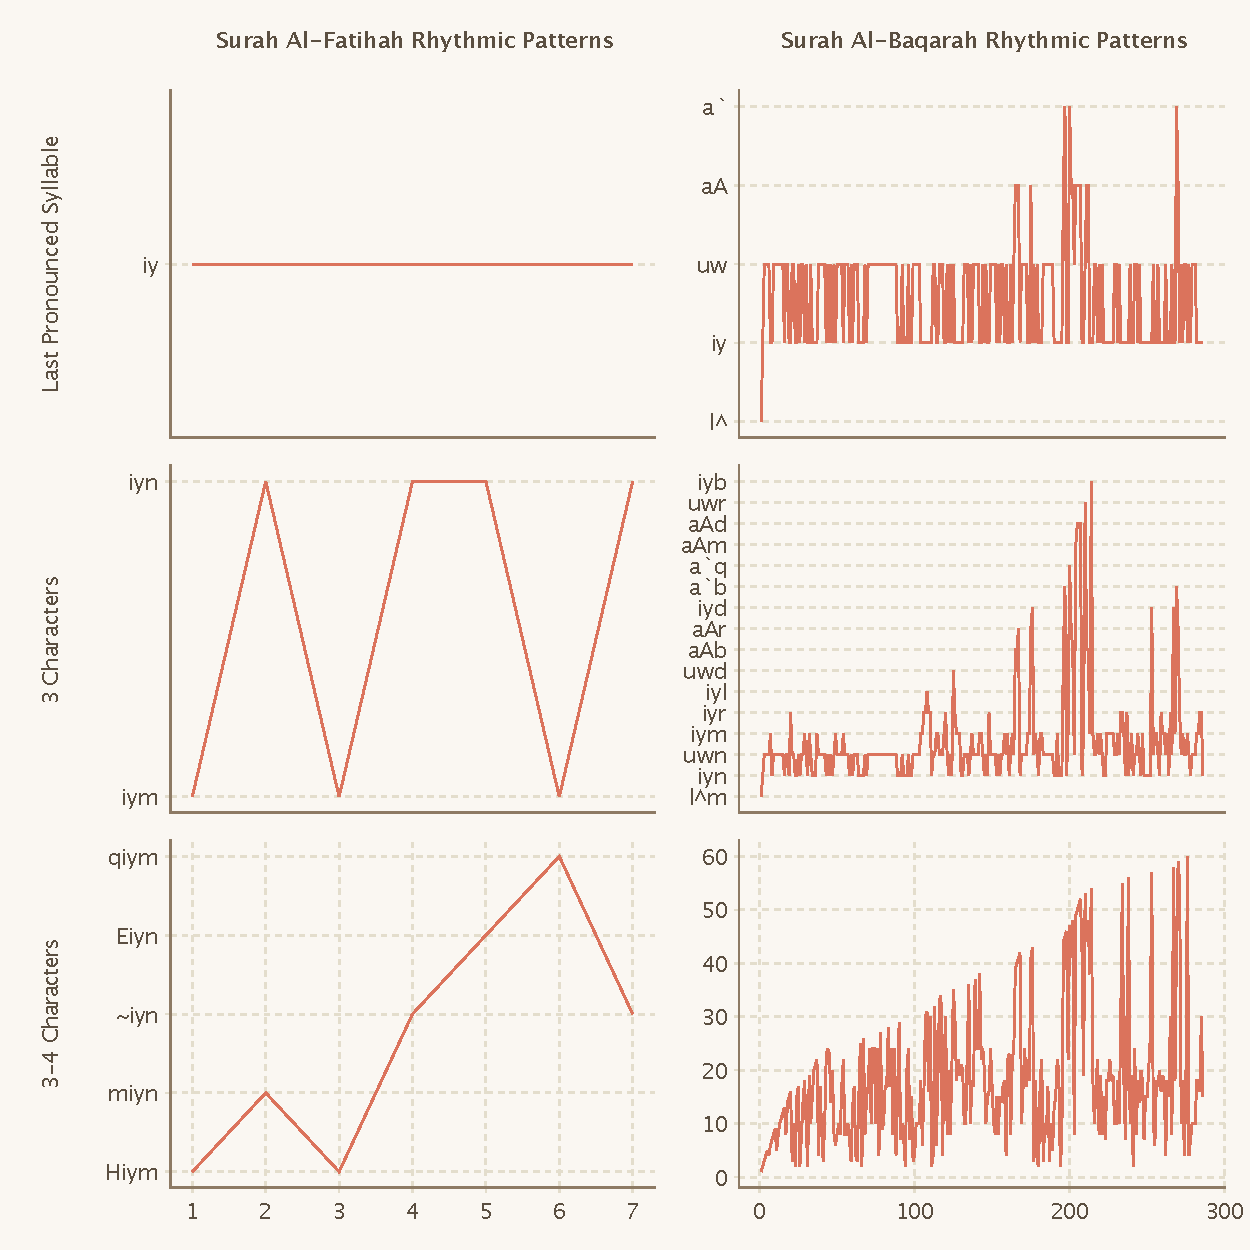
\includegraphics[width=\textwidth]{img/plot_rhythmic1.pdf}
    \caption{Rhythmic pattern of the last pronounced syllables of the \arb[trans]{sUraTu 'l-fati.haT} \arb{sUraTu 'l-fati.haT} and \arb[trans]{sUraTu 'l-baqaraT} \arb{sUraTu 'l-baqaraT}}
    \label{fig:fatihah_baqarah_rhythmic_method}
\end{figure}

With the data given in Figure \ref{fig:fatihah_baqarah_rhythmic_method}, we want to study if there are some interesting patterns on the switch of the rhythm, like in terms of topic, does the switch to particular rhythmic syllables imply a change in topic being discussed in the \arb[trans]{sUraT} \arb{sUraT}? Further, we also would want to model the dynamic of the changes using a statistical model. The first one is a non-dynamic model and is called Bayesian Networks model, and then the other one accounts the changes over the \arb[trans]{'ayaT} \arb{'ayaT} numbers, and this model is called the Discrete-Time Markov Models, both discussed in the succeeding sections after the concept of Graphical models, which is the basis of the said model.
\subsection{Directed Probabilistic Graphical Models (PGM)}
Probabilistic graphical models or simply graphical models are probability models represented graphically using nodes as random variables and segments or links as dependencies between variables. The link between the nodes is expressed as a chain rule of a conditional probability.

\begin{exmp}\label{exmp:directgraph}
Figure \ref{fig:baysnet} (a) illustrates the connections between three variables. The joint probability distribution of these random variables is expressed as follows:
$$
p(X_1,X_2,X_3)=p(X_1)p(X_2|X_1)p(X_3|X_1,X_2).
$$
On the other hand, Figure \ref{fig:baysnet} (b) has $N$ events namely $X_1,X_2,\cdots, X_N$, such that the joint probability is given by
$$
\begin{aligned}
p(X_1,X_2,\cdots,X_N)&=p(X_1)p(X_2)p(X_3|X_1,X_2)\cdots p(X_n|X_1,X_2)\\
&= p(X_1) p(X_2)\prod_{n=3}^{N} p(X_n|X_1,X_2).
\end{aligned}
$$
\end{exmp}
\begin{figure}
\begin{minipage}[c]{\textwidth}\centering
\begin{subfigure}[b]{.5\textwidth}
\centering
\begin{tikzpicture}[>=latex,auto,thick,node distance = 3cm]
\tikzstyle{every state}=[fill=white,draw=black,thick,text=black,scale=1]
\node[state] (A)  {$X_1$};
\node[state] (B) [above right of = A] {$X_2$};
\node[state] (C) [below right of = B] {$X_3$};
\path[->]
  (A) edge (B)
  (B) edge (C)
  (A) edge (C);
\end{tikzpicture}
\subcaption{Directed Acyclic Graph.}
\end{subfigure}\hspace{-1cm}
\begin{subfigure}[b]{.5\textwidth}
\centering
\begin{tikzpicture}[>=latex,auto,thick,node distance = 3cm]
\tikzstyle{every state}=[fill=white,draw=black,thick,text=black,scale=1]
\tikzstyle{plate}=[draw = black, rounded corners,thick,dashed, minimum width = 2cm, minimum height = 3cm, above]
\node (N) [plate] at (3,-1.3) {};
\node at (3,-1) {\footnotesize $3\to N$};
\node[state] (1) {$X_1$};
\node[state] (n) [right of = 1] {$X_n$};
\node[state] (2) [above of = n] {$X_2$};
\path[->]
  (1) edge (n)
  (2) edge (n);
%\draw[dotted, thick] ($(n)-(.5,.5)$) rectangle (1,1) node {$N$};
\end{tikzpicture}
\subcaption{Directed Acyclic Graph with Plate.}
\end{subfigure}
\end{minipage}
\caption[Bayesian Network Representation]{\it Bayesian Network Representation.}
\label{fig:baysnet}
\end{figure}
\begin{defn}[\it  Conditional Independence]
Let $X_1,X_2,$ and $X_3$ be a random variables, then $X_1$ and $X_2$ are said to be \textit{conditionally independent} given $X_3$, denoted by $X_1\CI X_2|X_3$ if
\begin{equation}
    p(X_1,X_2|X_3)=p(X_1)p(X_2)
\end{equation}
\end{defn}
\begin{exmp}
This example illustrates three possible cases that are likely to occur in probabilistic graphical models.
\textit{Case 1}: In Figure \ref{fig:case1} (a), $X_3$ is not known. The joint probability of the graph is given by
$$
 p(X_1,X_2,X_3)= p(X_3) p(X_1|X_3) p(X_2|X_3).
$$
It follows that $X_1\nCI X_2\mid \emptyset$, that is $X_1$ and $X_2$ are not independent since
\begin{figure}
\begin{minipage}[c]{\textwidth}
\centering
\begin{subfigure}[b]{.5\textwidth}
\centering
\begin{tikzpicture}[>=latex,auto,thick,node distance = 3cm]
\tikzstyle{every state}=[fill=white,draw=black,thick,text=black,scale=1]
\node[state] (A)  {$X_1$};
\node[state] (C) [above right of = A] {$X_3$};
\node[state] (B) [below right of = C] {$X_2$};
\path[->]
  (C) edge (A)
  (C) edge (B);
\end{tikzpicture}
\subcaption{$X_3$ is unknown.}
\end{subfigure}\hspace{-1cm}
\begin{subfigure}[b]{.5\textwidth}
\centering
\begin{tikzpicture}[>=latex,auto,thick,node distance = 3cm]
\tikzstyle{every state}=[fill=white,draw=black,thick,text=black,scale=1]
\tikzstyle{known} = [pattern = north west lines, pattern color = gray]

\node[state] (A)  {$X_1$};
\node[state] (C) [above right of = A, known] {$X_3$};
\node[state] (B) [below right of = C] {$X_2$};
\path[->]
  (C) edge (A)
  (C) edge (B);
\end{tikzpicture}
\subcaption{$X_3$ is known.}
\end{subfigure}
\end{minipage}
\caption[Tail-to-Tail Node Directed Graph]{\it Tail-to-Tail Node Directed Graph.}
\label{fig:case1}
\end{figure}
\vspace{.3cm}
$$
\begin{aligned}
 p(X_1,X_2)&=\sum_{\forall x} p(X_1,X_2,X_3=x)=\sum_{\forall x} p(X_3=x) p(X_1|X_3=x) p(X_2|X_3=x)\\
&\neq  p(X_1) p(X_2).
\end{aligned}
$$
However, if $X_3$ is known (see Figure \ref{fig:case1} (b)), $X_1\CI X_2\mid X_3$ because\vspace{.3cm}
$$
\begin{aligned}
 p(X_1,X_2|X_3)&=\frac{ p(X_1,X_2,X_3)}{ p(X_3)}=\frac{ p(X_3) p(X_1|X_3) p(X_2|X_3)}{ p(X_3)}\\
&= p(X_1|X_3) p(X_2|X_3).
\end{aligned}
$$\vspace{-.5cm}

\textit{Case 2}: Next consider the graph in Figure \ref{fig:case2} (a), the joint probability distribution factorizes into
$$
 p(X_1,X_2,X_3)= p(X_1) p(X_3|X_1) p(X_2|X_3).
$$
$X_1\nCI X_2\mid \emptyset$ since
$$
 p(X_1,X_2)=\sum_{\forall x} p(X_1) p(X_3=x|X_1) p(X_2|X_3=x)\neq  p(X_1) p(X_2).
$$
\begin{figure}
\begin{minipage}[c]{\textwidth}
\centering
\begin{subfigure}[b]{.5\textwidth}
\centering
\begin{tikzpicture}[>=latex,auto,thick,node distance = 3cm]
\tikzstyle{every state}=[fill=white,draw=black,thick,text=black,scale=1]
\node[state] (A)  {$X_1$};
\node[state] (C) [right of = A] {$X_3$};
\node[state] (B) [right of = C] {$X_2$};
\path[->]
  (A) edge (C)
  (C) edge (B);
\end{tikzpicture}
\subcaption{$X_3$ is unknown.}
\end{subfigure}\\[1cm]
\begin{subfigure}[b]{.5\textwidth}
\centering
\begin{tikzpicture}[>=latex,auto,thick,node distance = 3cm]
\tikzstyle{every state}=[fill=white,draw=black,thick,text=black,scale=1]
\tikzstyle{known} = [pattern = north west lines, pattern color = gray]

\node[state] (A)  {$X_1$};
\node[state] (C) [right of = A,known] {$X_3$};
\node[state] (B) [right of = C] {$X_2$};
\path[->]
  (A) edge (C)
  (C) edge (B);
\end{tikzpicture}
\subcaption{$X_3$ is known.}
\end{subfigure}
\end{minipage}
\caption[Head-to-Tail Node Directed Graph]{\it Head-to-Tail Node Directed Graph.}
\label{fig:case2}
\end{figure}
But if $X_3$ is known as in Figure \ref{fig:case2} (b) then $X_1\CI X_2\mid X_3$, that is\vspace{.2cm}
$$
\begin{aligned}
 p(X_1,X_2|X_3)&=\frac{ p(X_1,X_2,X_3)}{ p(X_3)}=\frac{ p(X_1) p(X_3|X_1) p(X_2|X_3)}{ p(X_3)}\\
&= \frac{ p(X_1) p(X_3|X_1)}{ p(X_3)} p(X_2|X_3)= p(X_1|X_3) p(X_2|X_3).
\end{aligned}
$$\vspace{-.5cm}

\textit{Case 3}: This case is a bit different from the preceding cases. Refer to the graphical model in Figure \ref{fig:case3} (a). The joint probability distribution of this graph is given by
$$
 p(X_1,X_2,X_3)= p(X_1) p(X_2) p(X_3|X_1,X_2).
$$
Previously, $X_1$ is not independent of $X_2$ if $X_3$ is unknown. That is not true for head-to-head relationship, however, since\vspace{.2cm}
$$
\begin{aligned}
 p(X_1,X_2)&=\sum_{\forall x} p(X_1) p(X_2) p(X_3=x|X_1,X_2)\\
&= p(X_1) p(X_2)\sum_{\forall x} p(X_3=x|X_1,X_2)= p(X_1) p(X_2).
\end{aligned}
$$
And so $X_1\CI X_2\mid \emptyset$. Also $X_1\nCI X_2\mid X_3$ as shown below\vspace{.2cm}
$$
\begin{aligned}
 p(X_1,X_2|X_3)&=\frac{ p(X_1,X_2,X_3)}{ p(X_3)}=\frac{ p(X_1) p(X_2) p(X_3|X_1,X_2)}{ p(X_3)}\\
&\neq p(X_1|X_3) p(X_2|X_3).
\end{aligned}
$$
\begin{figure}
\begin{minipage}[c]{\textwidth}
\centering
\begin{subfigure}[b]{.5\textwidth}
\centering
\begin{tikzpicture}[>=latex,auto,thick,node distance = 3cm]
\tikzstyle{every state}=[fill=white,draw=black,thick,text=black,scale=1]
\node[state] (C)  {$X_3$};
\node[state] (A) [above left of = C] {$X_1$};
\node[state] (B) [above right of = C] {$X_2$};
\path[->]
  (A) edge (C)
  (B) edge (C);
\end{tikzpicture}
\subcaption{$X_3$ is unknown.}
\end{subfigure}\hspace{-1cm}
\begin{subfigure}[b]{.5\textwidth}
\centering
\begin{tikzpicture}[>=latex,auto,thick,node distance = 3cm]
\tikzstyle{every state}=[fill=white,draw=black,thick,text=black,scale=1]
\tikzstyle{known} = [pattern = north west lines, pattern color = gray]

\node[state] (C) [known]  {$X_3$};
\node[state] (A) [above left of = C] {$X_1$};
\node[state] (B) [above right of = C] {$X_2$};
\path[->]
  (A) edge (C)
  (B) edge (C);
\end{tikzpicture}
\subcaption{$X_3$ is known.}
\end{subfigure}
\end{minipage}
\caption[Head-to-Head Node Directed Graph]{\it Head-to-Head Node Directed Graph.}
\label{fig:case3}
\end{figure}
\end{exmp}
\subsection{Markov Chain}\label{sec:markovchain}
Let $X_t,\;t=1,2,\cdots$ be a discrete-time stochastic process that takes values in the finite set $\mathscr{D}=\{\psi_1,\cdots,\psi_M\}$ called the \textit{states} of the system. In particular, define the probability distribution of the initial state as
\begin{equation}\label{eq:init}
\eta_{m}:= p(X_1=\psi_m)
\end{equation}
and the \textit{transition probabilities} from state to state as
\begin{equation}
\upsilon_{mm^{\star}}:= p(X_{t}=\psi_{m^{\star}}|X_{t-1}=\psi_{m},\cdots,X_1=\psi_1).
\end{equation}\vspace{-1cm}
\begin{defn}[\it  Markov Property]
A stochastic process is said to possess a \textit{Markov property} if the transition probability to state $m^{\star}$ given the history of the system, is equal to the probability of the $m^{\star}$th state given the immediate $m$th state. That is,
\begin{equation}
\label{eq:markov}
 p(X_{t}=\psi_{m^{\star}}|X_{t-1}=\psi_{m},\cdots,X_1=\psi_1):= p(X_{t}=\psi_{m^{\star}}|X_{t-1}=\psi_{m}).
\end{equation}
Suggesting that past and future states are conditionally independent given the present state.\end{defn}
\begin{remark}
A process having Markov property is called \textnormal{Markov process}. And the product of Equation (\ref{eq:markov}) over $t\in\{2,\cdots,\tau\}$ is called \textnormal{first-order Markov chain}.
\end{remark}

\begin{exmp}
Consider the Markov chain in Figure \ref{fig:markovgraph} (a) for four states. The graph is directed acyclic and so Proposition \ref{prop:d-sep} is equivalent to ``memorylessness'' Markov property. Suppose the history of the system from $t=1$ to $t = 3$ are the following states: $\psi_3,\psi_3$, and $\psi_2$. The transition probability from the current state $X_3=\psi_2$ to $X_4=\psi_4$ is given by
$$
\upsilon_{24}= p(X_4=\psi_4|X_3=\psi_2).
$$
The state $X_3$ has head-to-tail node relationship, so from Case 2 of Example \ref{exmp:directgraph} and Proposition \ref{prop:d-sep}, $X_2\CI X_4\mid X_3$ or $\psi_3\CI\psi_4\mid\psi_2$. 
\end{exmp}
This stochastic process is also called an \textit{observable} Markov chain since the output of the process is the set of states at each instant of time, where each state corresponds to a physical (observable) event (\cite{Rabiner89atutorial}). The state diagram in Figure \ref{fig:markovgraph} (b) is a directed cyclic graph (DCG). In this setting, the Markov property is not equivalent to Proposition \ref{prop:d-sep}, since $d$-separation will not hold. Also notice that the node is labelled as states as opposed to random variables in Figure \ref{fig:markovgraph} (a).
\begin{figure}[!t]
\centering
\begin{subfigure}[b]{\textwidth}
\centering
\begin{tikzpicture}[thick,node distance = 3cm]
\tikzstyle{every state}=[fill=white,draw=black,thick,text=black,scale=1]
\tikzstyle{known} = [pattern = north west lines, pattern color = gray]
\tikzstyle{plate}=[draw = black, rounded corners,thick, minimum width = 2cm, minimum height = 3.5cm, above]
\node (0) {\large\bf$\cdots\cdot$};
\node[state, known] (1)[right of = 0] {$X_4$};
\node[state, known] (2)[right of = 1] {$X_5$};
\node[state, known] (3)[right of = 2] {$X_6$};
\node (4)[right of = 3] {\large\bf$\cdots\cdot$};
\draw[
    >=latex,
%   every node/.style={above,midway},% either
    auto=right,                      % or
    loop above/.style={out=75,in=105,loop},
    every loop,
    ]
     %(1)   edge[loop above] node {$p_{gg}$}   (1)
     (0)   edge             node[above] {$\upsilon_{X_3X_4}$} (1)
     (1)   edge             node[above] {$\upsilon_{X_4X_5}$} (2)
     (2)   edge             node[above] {$\upsilon_{X_5X_6}$} (3)
     (3)   edge             node[above] {$\upsilon_{X_6X_7}$} (4);
\end{tikzpicture}
\subcaption{First-Order Markov Chain.}
\end{subfigure}\vspace{.6cm}
\begin{subfigure}[b]{\textwidth}
\centering
\begin{tikzpicture}[>=latex,auto,thick,node distance = 4cm]
\tikzstyle{every state}=[draw = black, rectangle, rounded corners,thick, scale = 1, above]
\tikzstyle{known} = [pattern = north west lines, pattern color = gray]

\node[state, known]    (1)                   		 	{$\psi_1$};
\node[state, known]    (2)[above right of=1]  		 	{$\psi_2$};
\node[state, known]    (4)[below right of=1]   		{$\psi_4$};
\node[state, known]    (3)[below right of=2]    {$\psi_3$};
\path[->]
(1) edge[loop left]        node{$\upsilon_{11}$} (1)
    edge[bend left]        node{$\upsilon_{12}$} (2)
    edge[bend left]        node{$\upsilon_{14}$} (4)
(2) edge[loop above]       node{$\upsilon_{22}$} (2)
	edge[bend left]        node{$\upsilon_{23}$} (3)
	edge[bend left]        node{$\upsilon_{21}$} (1)
(3) edge[loop right]       node{$\upsilon_{33}$} (3)
	edge[bend left]        node{$\upsilon_{34}$} (4)
	edge[bend left]        node{$\upsilon_{32}$} (2)
(4) edge[loop below]       node{$\upsilon_{44}$} (4)
    edge[bend left] 	   node{$\upsilon_{41}$} (1)
    edge[bend left]        node{$\upsilon_{43}$} (3);
\end{tikzpicture}
\subcaption{State Transition Diagram.}
\end{subfigure}
\caption[Markov Chain Graphs]{\it Markov Chain Graphs.}
\label{fig:markovgraph}
\end{figure}
\section{Thematic Analysis}
This section will discuss the methodology on how to extract the themes or topics of an input text like a \arb[trans]{sUraT} \arb{sUraT}. There are two approaches for this, using the classic statistical methodology and using the recent large language models. The popular statistical method for this is using a Bayesian model called Latent Dirichlet Allocation or LDA. On the other hand, there are two for large language model, and that is using a Bidirectional Encoder Representation from Transformers (BERT) and Generative Pre-Trained Transformer (GPT). The three approaches will be tested for generating these topics.
\subsection{Latent Dirichlet Allocation}\label{sec:lda}
Latent Dirichlet Allocation (LDA) is a Statistical methodology that is based on Bayesian inference \cite{bayes,laplace1986}. It is a generative probabilisitic model for collection of discrete data such as text corpora \cite{blei2003latent}. The main formula is defined below:
\begin{defn}[\it Latent Dirichlet Allocation]
Let $\mathbf{W},\mathbf{Z},\boldsymbol{\theta},\boldsymbol{\varphi}$ be the random variables, and let $\alpha$ and $\beta$ be the hyper-parameters, then the probability of generating a document is
\begin{equation}
    \mathbb{P}(\mathbf{W},\mathbf{Z},\boldsymbol{\theta},\boldsymbol{\varphi})=\prod_{j=1}^m\mathbb{P}(\boldsymbol{\theta}_j;\alpha)\prod_{i=1}^{k}\mathbb{P}(\boldsymbol{\varphi};\beta)\prod_{t=1}^{n}\mathbb{P}(\mathbf{Z}_{j,t}|\boldsymbol{\theta}_j)\mathbb{P}(\mathbf{W}_{j,t}|\boldsymbol{\varphi}_{\mathbf{Z}_{j,t}})
\end{equation}
\end{defn}
\subsection{Large Language Models}\label{sec:llm_method}
Generative Artificial Intelligence or GenAI for short has been making waves on its effectiveness to generate texts, images, audio, video, etc. It has elevated humanity to a new level of capability. However, behind this amazing capabilities is that GenAI is by design a mathematical formula that are called \textit{model}. There are several types of \textit{models}, and one of those is the Large Language Model (LLM). The following section will discuss what LLM is and its mathematical formulation.
\subsection{Bidirectional Encoder Representation from Transformers}\label{sec:bert}
BERT or Bidirectional Encoder Representation from Transformers model is a large language model proposed by \citeA{devlin2018bert}. From the name itself, it is based on the Transformer model architecture (\textit{see} discussion in Section \ref{sec:transformers}) in that it only uses the Encoder layer, and stack it together. BERT was pre-trained on large corpus of text using two unsupervised (\textit{see} Section \ref{sec:unsupervised_models}) tasks, and these are:
\begin{enumerate}
    \item \textit{Masked Language Modeling (MLM)} - tokens (\textit{see} Section \ref{sec:text_tokenization}) are randomly masked in the input and trains the model to predict these masked tokens based on the surrounding context.
    \item \textit{Next Sentence Prediction (NSP)} - tains the model to understand the relationship between two sentences by predicting if one sentence follows the other.
\end{enumerate}
After pre-training the model, BERT can then be fine-tuned on specific tasks like question answering, sentiment analysis, and more with relatively smaller datasets. With that, BERT works as follows: 
\begin{enumerate}
    \item \textit{Input Representation} - BERT takes tokenized text as input, which includes a pair of sentences. The input is converted into tokens, added with special tokens like [CLS] (classification token at the beginning) and [SEP] (separator token between sentences).
    \item \textit{Embedding Layer} - The tokens are converted into embeddings which are the sum of token embeddings, segment embeddings, and position embeddings.
    \item \textit{Encoder Layers} - The embeddings are then passed through multiple layers of bidirectional Transformer encoders (\textit{see} Section \ref{sec:transformers}), which apply self-attention mechanisms to generate contextualized representations for each token.
    \item \textit{Output} - The final hidden states from the encoder layers are used for different tasks:
    \begin{itemize}
        \item The [CLS] token’s representation can be used for classification tasks.
        \item The representations of other tokens can be used for tasks like named entity recognition (NER) or question answering.
    \end{itemize}
\end{enumerate}
There are several applications of BERT model, but for this paper it will be used for Topic Modeling and Text Summarization of the Qur'\=an. In particular, CL-AraBERT model by will be used for extracting embeddings of the Qur'\=anic words for further analysis.
\subsection{Generative Pre-Trained Transformer}
GPT or Generative Pre-Trained Transformer is another large language model proposed by \cite{radford2018improving}. From the name itself and like BERT, GPT is based on the Transformer model \cite{vaswani2017attention}, \textit{see} Section \ref{sec:transformers}. Unlike BERT though, GPT uses the decoder layer of the Transformer model and stacks it multiple times. This is the model that is powering the ChatGPT\footnote{\url{https://chat.openai.com/}} of OpenAI and also Claude AI\footnote{\url{https://claude.ai/}} of Anthropic\footnote{\url{https://anthropic.com/}}.

GPT models like those powering ChatGPT were pre-trained on large corpora by going through the sequence of the texts in \textit{unidirection}, which is contrary to the \textit{bidirectional} approach of BERT model. As such, the GPT models excel in generating text and performing tasks that require producing coherent sequences of words, in applications like text completion and creative writing. Whereas BERT is technically effective for tasks requiring deep contextual understanding such as text classification and named-entity recognition.

For this paper, the 
\section{Concentrism Statistical Formulation}
One of the specific items for the second objective of this paper is on the theory of concentrism, and how can this be formulated statistically, and what are the insights that can be extracted. The idea of the theory of concentrism is that a given texts with define partition follows a ring or concentric structure, which is a literary form where the text is organized in such a way that it mirrors itself around a central point. This means that the beginning and ending sections correspond to each other, moving inward until the center of the text, which often contains the main message or theme. This particular pattern was observed by linguistic experts that it got documented in a book by \citeA{farrin2014structure}. This theory can be defined mathematically as follows:

\begin{defn}[\it Concentric]\label{defn:concentric}
    Let $\mathscr{D}$ be a collection of texts, then $\mathscr{D}$ is said to have a \textit{concentric} or \textit{ring} structure if and only if $\exists\;\mathscr{A}_i\subseteq\mathscr{D},\mathscr{C}\subseteq\mathscr{D},$ and $\mathscr{A}_i^{*}\subseteq\mathscr{D},i\in\mathbb{N}_1$; and that these sets are arranged as follows in $\mathscr{D}$:  $\mathscr{A}_1,\cdots,\mathscr{A}_n,\mathscr{C},\mathscr{A}_1^{*},\cdots,\mathscr{A}_n^{*}$, such that $\mathscr{A}_i^{*}$ \underline{mirrors} $\mathscr{A}_i$ in semantic, and that $\mathscr{C}$ is the center texts of the document $\mathscr{D}$ that is \underline{not related} to both $\mathscr{A}_i$ and $\mathscr{A}_i^{*}$.
\end{defn}

The underlined words above will be used in the next section, because mathematically it begs further definition on what we mean by "mirrors" and "not related" mathematically. This will be defined in the next section. Now, another pattern that was observed by \citeA{farrin2014structure} as chiasmus, which is basically \textit{ring} structure but the second half of the ring after the center is the "complement" or "reversal" of the first half of the document before the center. The following is its mathematical definition.

\begin{defn}[\it Chiasmus]\label{defn:chiasmus}
    Let $\mathscr{D}$ be a collection of texts, then $\mathscr{D}$ is said to have a \textit{concentric} or \textit{ring} structure if and only if $\exists\;\mathscr{A}_i\subseteq\mathscr{D},\mathscr{C}\subseteq\mathscr{D},$ and $\mathscr{A}_i^{*}\subseteq\mathscr{D},i\in\mathbb{N}_{geq 1}$; and that these sets are arranged as follows in $\mathscr{D}$:  $\mathscr{A}_1,\cdots,\mathscr{A}_n,\mathscr{C},\mathscr{A}_1^{c},\cdots,\mathscr{A}_n^{c}$, such that $\mathscr{A}_i^{c}$ is the \underline{complement} or \underline{reversal} of $\mathscr{A}_i$ in semantic, and that $\mathscr{C}$ is the center texts of the document $\mathscr{D}$ that is \underline{not related} to both $\mathscr{A}_i$ and $\mathscr{A}_i^{c}$.
\end{defn}
There are other structures that can be observed in the Qur'\=an, like \textit{parallelism} where themes are repeated in other \arb[trans]{sUraT} \arb{sUraT}; and \textit{segment structure}, where a particular segment starts and ends with similar phrases or themes, creating a bracket around the content; but, these other structures are not studied in this paper. Apart from this, there is also the "mathematical patterns" of the Qur'\=an which has been extensively studied by \citeA{rashad1981}, but this is also not studied in this paper.
\subsection{Cosine Similarity}
From Defn. \ref{defn:concentric} and \ref{defn:chiasmus}, there are key words that are still vagued in terms of its mathematical meaning, and these were "mirrors," "not related," and "complemented" or "reversal." Well, semantically these words refer to measurement, particularly, a distance measurement. So that, "mirrors" would mean related meaning the distance in terms of measurement should be relatively close as opposed to "not related" or "complemented" or "reversal". So, how to measure this then?

The answer to the above question is by measuring the distance of their word embeddings. These embeddings as discussed in Section \ref{sec:bert} will be extracted from BERT models. Using these embeddings a similarity or distance measurement can be used, and the common formula for this is the \textit{cosine similarity} defined below.

\begin{defn}[\it Cosine Similarity]
    Let $\mathbf{u}:=[u_1,\cdots,u_n]^{\text{T}}$ and $\mathbf{v}:=[v_1,\cdots,v_n]^{\text{T}},\linebreak n\in\mathbb{N}_{\geq 1}$ be word embedding vectors such that $\theta_{\mathbf{u},\mathbf{v}}$ is the angle between $\mathbf{u}$ and $\mathbf{v}$, then the cosine similarity of the given angle $\theta$ is
    \begin{equation}
        \cos(\theta_{\mathbf{u};\mathbf{v}}):=\frac{\mathbf{u}\cdot\mathbf{v}}{||\mathbf{u}||\,||\mathbf{v}||}.
    \end{equation}
\end{defn}
Therefore, for this study, if $\theta_1$ is the angle between "related" \arb[trans]{'Ayat} \arb{'Ayat} embeddings, and $\theta_2$ is the angle between "not related" \arb[trans]{'Ayat} \arb{'Ayat} embeddings, then it should be expected that $\cos(\theta_1)\leq\cos(\theta_2)$. Further, if $\theta_3$ is the angle of "complemented" or "reversal" \arb[trans]{'Ayat} \arb{'Ayat} embeddings, then maybe $\cos(\theta_1)\leq\cos(\theta_3)$ since it is not clear yet how disparate is the "related" distance to "complement" or "reversal" distance, and this is especially true for the relation of $\theta_2$ to $\theta_3$ as it cannot be determined up front, and may only be observed from the data, which will be discussed in the next chapter.
\subsection{Bayesian Optimization}
From Defn. \ref{defn:concentric} and \ref{defn:chiasmus}, it both states that, a document $\mathscr{D}$ may only be considered \textit{concentric} or \textit{chiasmus} if and only if "there exist", denoted by the symbol $\exists$. Indeed, subset of texts $\mathscr{A}_i$s, $\mathscr{C}$, and $\mathscr{A}_i^{*}$ or $\mathscr{A}_i^{\text{c}}$ are all determined manually by the investigator. In this study, we propose to automate the determination of these subsets of texts of document $\mathscr{D}$, and this is through the use of an optimization algorithm called Bayesian Optimization. The idea behind Bayesian optimization is that it approximates the objective function with a \textit{surrogate} function, and using this surrogate to find the global maximum or minimum of the objective function. Furthermore, it does this by fitting the surrogate function to the objective function in as few input points or iteration as possible. As such, an \textit{acquisition} function is needed for choosing smartly the next input points to be used for fitting the surrogate. Using these components, a Bayes' Theorem is used in fitting the surrogate.

To do this, a \textit{global objective function} must be defined, for this study, the cosine similarity discussed in the previous section will be used as the said cost function that will either be maximized or minimized. The core model for this optimization is the Gaussian Process defined below.
\subsubsection{Surrogate Function}
The surrogate function aims to approximate the objective function. In Bayesian, optimization, the surrogate function is defined by the Gaussian process (GP).
\begin{defn}[\it Gaussian Process]\label{defn:gp}
    Let $Y_1,Y_2,\cdots,Y_T$ be sequence of random variables such that $Y_t\in\mathbf{Y}$, then the sequence is a \textit{Gaussian process} (GP) if and only if $\mathbf{Y}\overset{\mathrm{iid}}{\sim}\mathcal{N}(\boldsymbol{\mu}, \boldsymbol{\Sigma})$.
\end{defn}
\begin{defn}[\it Parameter Space]\label{defn:parameter_space}
    Let $\mathbf{s}_i\in\mathscr{D}$ be a word embedding of an \arb[trans]{'ayaT} \arb{'ayaT} in document $\mathscr{D}$, which can be a \arb[trans]{sUraT} \arb{sUraT}, group of \arb[trans]{suwar} \arb{suwar}, or group of \arb[trans]{'Ayat} \arb{'Ayat} within a \arb[trans]{sUraT} \arb{sUraT}. Further, suppose $\mathscr{A}_i,\mathscr{C},\mathscr{A}_i^{*}\subseteq\mathscr{D}$ such that $\mathscr{A}_i:=\{\mathbf{s}_{i,1},\cdots,\mathbf{s}_{i,n}\},\linebreak\mathscr{C}:=\{\mathbf{s}_{n+1},\cdots,\mathbf{s}_{n+c}\}$, and $\mathscr{A}_i^{*}:=\{\mathbf{s}_{i,(n+c+1)},\cdots,\mathbf{s}_{i,(n+c+n)}\}$, then the \textit{parameters} to be optimized are assigned to $\mathbf{v}:=[n,c]^{\text{T}}$, and since $n,c,m\in\mathbb{N}_{\geq 2}$, then the \textit{parameter space} is $\mathscr{P}:=\mathbb{N}_{\geq 2}\times\mathbb{N}_{\geq 2}\times\mathbb{N}_{\geq 2}=(\mathbb{N}_{\geq 2})^3$, so that $\mathbf{v}\in\mathscr{P}$. 
\end{defn}
\begin{defn}[\it Semi-Circle Cost Function]\label{defn:semi_circle_cost}
    From Defn. \ref{defn:parameter_space}, let $r_1$ to denote that $\mathscr{A}_i$ is "related" to $\mathscr{A}_i^{*}$, and $r_2$ to denote that $\mathscr{A}_i$ is "reversal" of $\mathscr{A}_i^{*}$, such that $\eta:=\{r_1,r_2\}$, then  the \textit{semi-circle} cost function between $\mathscr{A}_i$ and $\mathscr{A}_i^{*}$ is defined as:
    \begin{equation}
        \operatorname{\gamma}_{a}(\mathbf{v};\mathscr{A}_i,\mathscr{A}_i^{*},\eta):=\begin{cases}
            \frac{1}{n}\sum_{k=1}^{n}\cos\left(\theta_{\mathbf{s}_{i,k};\mathbf{s}_{i,n+l}}\right),&\text{if}\;\eta=r_1\\
            1-\frac{1}{n}\sum_{k=1}^{n}\cos\left(\theta_{\mathbf{s}_{i,k};\mathbf{s}_{i,n+l}}\right),&\text{if}\;\eta=r_2\\
        \end{cases}
    \end{equation}
\end{defn}
\begin{defn}[\it Center Cost Function]\label{defn:center_cost}
    From Defn. \ref{defn:parameter_space}, the \textit{center} cost function is defined as:
    \begin{equation}
        \operatorname{\gamma}_{b}(\mathbf{v};\mathscr{A}_i,\mathscr{C},\mathscr{A}_i^{*}):=2-\frac{1}{nc}\sum_{k=1}^{n}\sum_{l=1}^{c}\cos\left(\theta_{\mathbf{s}_{i,k};\mathbf{s}_{n+l}}\right)-\frac{1}{nc}\sum_{k=1}^{n}\sum_{l=1}^{c}\cos\left(\theta_{\mathbf{s}_{n+l};\mathbf{s}_{i,n+c+k}^{*}}\right).
    \end{equation}
\end{defn}
\begin{defn}[\it Global Cost Function]\label{defn:global_cost}
    From Defn. \ref{defn:parameter_space}-\ref{defn:center_cost}, the \textit{global} cost function is defined as:
    \begin{equation}
        \operatorname{\gamma}_{g}(\mathbf{v};\mathscr{A}_i,\mathscr{C},\mathscr{A}_i^{*},\eta):=\operatorname{\gamma}_{a}(\mathbf{v};\mathscr{A}_i,\mathscr{A}_i^{*},\eta)+\operatorname{\gamma}_{b}(\mathbf{v};\mathscr{A}_i,\mathscr{C},\mathscr{A}_i^{*})
    \end{equation}
\end{defn}
\begin{defn}[\it Optimal Parameters] From Defn. \ref{defn:global_cost}, the optimal parameters would be:
\begin{equation}
    \hat{\mathbf{v}}:=\underset{n,c}{\arg\min}\operatorname{\gamma}_{g}(\mathbf{v};\mathscr{A}_i,\mathscr{C},\mathscr{A}_i^{*},\eta),
\end{equation}    
\end{defn}
\begin{prop}\label{prop:hypedist}
    Let $\mathscr{P}$ be the parameter space and suppose $\gamma(\mathbf{v})\overset{\mathrm{iid}}{\sim}\mathcal{N}(m(\mathbf{v}),k(\mathbf{v},\mathbf{v})), \linebreak\forall \mathbf{v}\in\mathscr{P}$, then for any $\boldsymbol{\delta}:=[\gamma(\mathbf{v}_1),\cdots,\gamma(\mathbf{v}_n)]^{\top}$, $\boldsymbol{\delta}\overset{\mathrm{iid}}{\sim}\mathcal{N}_n(\mathbf{m},\mathbf{K})$, where 
    \begin{equation}
        \mathbf{m}:=[m(\mathbf{v}_1),\cdots,m(\mathbf{v}_n)]^{\top}
    \end{equation}
    and
    \begin{equation}
        \mathbf{K}:=\left[\begin{matrix}
        k(\mathbf{v}_1,\mathbf{v}_1)&\cdots&k(\mathbf{v}_1,\mathbf{v}_n)\\
        \vdots&\ddots&\vdots\\
        k(\mathbf{v}_n,\mathbf{v}_1)&\cdots&k(\mathbf{v}_n,\mathbf{v}_n)\\
        \end{matrix}\right]
    \end{equation}
\end{prop}
\begin{proof}
    The proof follows from the proof of Theorem 1.2.9 of \citeA{muirhead2005}.
\end{proof}
\begin{remark}
    From Proposition \ref{prop:hypedist} and Definition \ref{defn:gp}, $\boldsymbol{\delta}$ is a GP.
\end{remark}
\begin{prop}\label{prop:jointpdf}
    From Proposition \ref{prop:hypedist}, suppose $\boldsymbol{\delta}_{*}:=[\gamma(\mathbf{v}_{n+1}),\cdots,\gamma(\mathbf{v}_{n+p})]^{\top}$, such that $\boldsymbol{\delta}_{*}\overset{\mathrm{iid}}{\sim}\mathcal{N}_p(\mathbf{m}_*,\mathbf{K}_*)$ then 
    \begin{equation}
        \left[
        \begin{matrix}
            \boldsymbol{\delta}\\
            \boldsymbol{\delta}_{*}\\
        \end{matrix}
        \right]\overset{\mathrm{iid}}{\sim}
        \mathcal{N}_{n+p}\left(\left[
        \begin{matrix}
            \mathbf{m}\\
            \mathbf{m}_{*}\\
        \end{matrix}
        \right],\left[
        \begin{matrix}
            \mathbf{K}&\mathbf{K}_{*}\\
            \mathbf{K}_{*}^{\top}&\mathbf{K}_{**}\\
        \end{matrix}
        \right]\right)
    \end{equation}
\end{prop}
\begin{proof}
    Let $\mathbf{u}:=[\boldsymbol{\delta},\boldsymbol{\delta}_{*}]^{\top}$, then $\mathbf{u}=[\gamma(\mathbf{v}_1),\cdots,\gamma(\mathbf{v}_{n+p})]^{\top}$. Further, since $\mathbf{\gamma}(\mathbf{v}_i)\overset{\mathrm{iid}}{\sim}\mathcal{N}(m(\mathbf{v}_i),k(\mathbf{v}_i,\mathbf{v}_i)),\forall i\in\mathbb{N}_{\leq n+p}$, then the joint distribution of the $\gamma(\mathbf{v}_i)$s, i.e. $\mathrm{Pr}(\mathbf{u})$, follows from the proof of Theorem 1.2.9 of \citeA{muirhead2005}.
\end{proof}
\begin{cor}\label{cor:condpdf}
From Proposition \ref{prop:jointpdf}, let $\mathbf{m}$ and $\mathbf{m}_{*}$ be zero vectors, then the following conditional distribution is true:
    \begin{equation}\label{eq:gp_updater}    \boldsymbol{\delta}_*\mid\boldsymbol{\delta}\overset{\mathrm{iid}}{\sim}\mathcal{N}_{p}(\mathbf{K}_{*}^{\top}\mathbf{K}^{-1}\boldsymbol{\delta},\mathbf{K}_{**}-\mathbf{K}_{*}^{\top}\mathbf{K}^{-1}\mathbf{K}_{*}).
\end{equation}
\end{cor}
\begin{proof}
    The proof follows by reversing the condition from $\mathbf{X}_1\mid\mathbf{X}_2$ to $\mathbf{X}_2\mid\mathbf{X}_1$ of the proof of Theorem 1.2.11 of \cite{muirhead2005}.
\end{proof}
\begin{defn}[\it Lower Confidence Bound]\label{defn:lcb}
    Let $m(\mathbf{v})$ be the mean of the GP, then the Lower Confidence Bound (LCB) notated as $\xi$ is given by
    \begin{equation}
        \xi(\mathbf{v}\mid\zeta):=m(\mathbf{v})-\zeta k(\mathbf{v},\mathbf{v}),
    \end{equation}
    where $\zeta$ is the balancing factor.
\end{defn}
The \textit{global cost} computed from the global cost function in Defn. \ref{defn:global_cost} is approximated by the Gaussian process (the surrogate function) defined in Defn. \ref{defn:gp} through Proposition \ref{prop:hypedist}. So that, for any new observed global cost computed from the new parameter input $\mathbf{v}$, chosen by the acquisition function defined in Defn. \ref{defn:lcb}, the joint distribution with the previous global cost is given in Proposition \ref{prop:jointpdf}. Therefore, computing for the conditional distribution of the new global costs conditioned on previous global cost is given in Corollary \ref{cor:condpdf}. The process of acquiring new parameter candidate and computing the global cost is done iteratively. The algorithm converges until there is no significant changes on the new parameter candidate relative to the preceding parameter candidate, or alternatively, until a specified maximum iteration.
\begin{center}
    \textcolor{red}{add theoretical Bayes theorem computations here}
\end{center}
\section{Integrating Other Islamic Literatures}
The third objective of this paper asks on how to unify all of these results from Statistics, Machine Learning, AI, and the work of Islamic scholars on Qur'\=anic studies help in understanding the Qur'\=an. Discussions on this will be provided in the next chapter, but in terms of the methodology on how to combine all of this into something that is accessible to Muslims and those interested in learning the Qur'\=an, this paper will provide the architecture on how to package all of these.

The idea of combining the results in this paper with the work of Islamic scholars requires some form of relation, that is, relating particular results to what was studied by the scholars before in order to provide more context. For such tasks, of relating particular result to a large corpus of documents written in Qur'\=anic studies will seem to be a great endeavor. Manually reading through those corpus and combining to the results of this paper, plus trying to summarize all of this combinations can be a daunting task. Fortunately, at the age of Generative AI, such task can be automated. To do this, there are three main components, and these are: 
\begin{enumerate}
    \item Digitized Pre-Modern Islamic Documents - this include like the \textit{ahadith} or the traditions or \arb[trans]{sunnaT} \arb{sunnaT} of the Prophet, and writings of the early Islamic scholars.
    \item Information Retrieval Algorithm - an algorithm that will help extract the necessary pre-modern Islamic document related to the results.
    \item Text Summarizer - a generative AI model that can create coherent summary on the combinations of the results of this paper plus the context from the pre-modern Islamic document
\end{enumerate}
\subsection{Open Islamic Text Initiative}
The OpenITI or Open Islamic Text Initiative project by Aga Khan University, Institute for the Study of Muslim Civilisations in London, Roshan Institute for Persian Studies at the University of Maryland, College Park, and Universität Hamburg is a huge step to computational analysis of the Islamicate texts, which include the pre-modern Islamic texts. What the team of this project did is that they converted all of the said documents into a text file, so that, it can be used for any digital humanities study of these texts.

According to their About page in their website\footnote{\url{https://openiti.org/}}, since its founding in 2016, OpenITI's work has focused on the tasks necessary to build digital capacity in Islamicate studies, including improving Arabic-script optical character recognition (OCR) and handwritten text recognition (HTR), developing robust Arabic-script standards for OCR and HTR output and text encoding, and creating platforms for the collaborative creation of Islamicate text corpora and digital editions.

More specifically, OpenITI compiled all of these digitized texts in their sub-project called KITAB or Knowledge, Information Technology, and the Arabic Book. For this paper, the digitized Sahih al-Bukhari from  OpenITI's KITAB will be used as the Islamic context for demonstrating how to combine the results from this study. Fortunately, a Julia library called Kitab.jl\footnote{\url{https://github.com/alstat/Kitab.jl}} developed by \citeA{al_ahmadgaid_b_asaad_kitab} was made to interface with KITAB books for easy access, and will be used for this project.
\subsection{Retrieval-Augmented Generation}
The popularity of Generative AI like ChatGPT has made the said tool the go-to assistant when it comes to anything writing. It is especially good at synthesizing different texts and summarizing it beautifully. However, like any \textit{mathematical models}, it only has knowledge about the data it was trained on. In fact, those that it even learned has the chance of getting it wrong. This is just the nature of models in general, they are not perfect but good enough to be an effective assistant. Therefore, when it comes to new informations, or data, these AI models can still generate answers that seem believable when in fact it is not, and this is what is called as \textit{AI hallucination}. So the question now is, how can we at least mitigate this limitation and still be able to take advantage its creative writing skills? Well, the simplest way is to provide it more context. Like instead of just asking a question to it, provide it with a document as an attached context for it to read, so that, it can provide its answer not only based on the knowledge it learned during the training, but also the documents provided to it in the query. This will make the AI generate a better and more relevant answer.

Now, the next question is, if there are several documents, how can someone automate the process where the user will only query, and then the AI will be given the necessary document it needs for the context, plus those documents that are related to the query can also be presented as part of the outputs? Well, this is the concept of Retrieval-Augmented Generation or RAG. This method proposed by \citeA{NEURIPS2020_6b493230} is gaining popularity especially in companies trying to integrate AI into their workflow.
\begin{center}
    \textcolor{red}{add figure here in the context of the methodology proposed}
\end{center}
\section{Programming Languages Setup}\label{sec:code_setup}
This section will discuss the programming languages used in this paper. As mentioned in Chapter \ref{ch:introduction}, there are three main programming languages that will be used, all of which are known in the area of data analysis, and these are Julia, Python, and R. The rule of thumb here is to use Julia as much as possible. With that said, Python is the popular framework for deep learning modeling, and therefore will be used in this paper for such tasks if in case the deep learning model is not available in Julia. Finally, R is known for almost all statistical models, especially those that are very niche, and this is because R was created as a statistical software not as a general purpose programming language like Julia and Python. To download these software, refer to Table \ref{tbl:download_page} for the links to the download page. Further, there are several tutorials on these programming languages in Youtube\footnote{\url{https://www.youtube.com/}} for those interested to learn these. Finally, all of the codes for this paper are stored in a Github repository below:

\begin{center}
    \url{https://github.com/alstat/ma-thesis/tree/main/codes}
\end{center}

Further, in terms of the libraries used, QuranTree.jl\footnote{\url{https://github.com/alstat/QuranTree.jl}} by \citeA{asaad2021qurantree} will be used as the main library for interfacing with the digitized Qur'\=an text; Yunir.jl\footnote{\url{https://github.com/alstat/Yunir.jl}} by \citeA{al_ahmadgaid_b_asaad_yunir} will be used for text analytics; Kitab.jl\footnote{\url{https://github.com/alstat/Kitab.jl}} by \citeA{al_ahmadgaid_b_asaad_kitab} will be used for interfacing with other Islamicate texts from OpenITI\footnote{\url{https://openiti.org/}}.
\begin{table}[!t]
    \caption{Download page for programming languages used}
    \begin{tabularx}{\textwidth}[h]{XXl}
        \toprule
        Software&Version&Download Page\\
        \midrule
        Julia&1.10.3&\url{https://julialang.org/downloads/}\\
        Python&3.12.2&\url{https://www.python.org/downloads/}\\
        R&3.4.4&\url{https://cran.r-project.org/bin/windows/base/}\\
        \bottomrule
    \end{tabularx}
    \label{tbl:download_page}
\end{table}
\chapter{Results and Discussions}\label{ch:results}
This chapter is organized as follows: Section \ref{sec:result_data} will discuss the main data used in this study, including an illustration of how to access it and the features it provides; Section \ref{sec:ch4_desc_stat} will discuss the results of the descriptive statistics; Section \ref{sec:ch4_morphological_analysis} will discuss the results on the morphological analyses; Section \ref{sec:ch4_structural_analysis} will discuss the results on the structural analyses; Section \ref{sec:ch4_topic_modeling_result} will discuss the results of the topic modeling; and Section \ref{sec:ch4_relating_islamic_texts} will discuss the results of relating the Qur'\=an to other Islamic texts and analyses. Finally, Section \ref{sec:ch4_limitations} will discuss the limitations of the models used in this study.
\section{Qur'\=an Data}\label{sec:result_data}
The main data used in this study is the digitized Qur'\=an data available through QuranTree.jl library by \citeA{asaad2021qurantree}. QuranTree.jl has both the Tanzil data\footnote{\url{https://tanzil.net/}} and the Qur'anic Arabic Corpus\footnote{\url{https://corpus.quran.com/}}, where the latter contains the morphological data of the Qur'\=an. These digital data will help in doing programmatic analyses of the Qur'\=an using Julia programming language. To see how to access this in QuranTree.jl in Julia, Figure \ref{fig:result_crps_tbl} shows the code for accessing the morphological data of the first \arb[trans]{'ayaT} \arb{'ayaT} of \arb[trans]{sUraTu 'l-fAti.haT} \arb{sUraTu 'l-fAti.haT}. Note that, the setup on how to install the said QuranTree.jl and other libraries and the Julia programming language is given in Appendix \ref{appendix:installation_libraries}.

Referring to Figure \ref{fig:result_crps_tbl}, the first line of the code, which has the code \texttt{using QuranTree}, loads the QuranTree library. The second line, which has the code \texttt{crps, tnzl = load(QuranData())}, loads both the morphological data and the Tanzil data of the Qur'\=an. The third line of the code converts these data into a tabular form. Finally, the fourth line of the code queries the first \arb[trans]{sUraT} \arb{sUraT} and the first \arb[trans]{'ayaT} \arb{'ayaT} of the morphological data of the Qur'\=an, the results of which are shown in succeeding lines with the heading indicating \texttt{Chapter 1} and \texttt{Verse 1}. Both the number 1 for Chapter 1 is indicated by \texttt{[1]} and \texttt{[1]}, respectively, in the code \verb|crps_tbl[1][1]| in Figure \ref{fig:result_crps_tbl}.

\begin{figure}[!t]
    \centering
    \includegraphics[width=\textwidth]{img/crps_tbl.png}
    \caption{\arb[trans]{sUraTu 'l-fAti.haT} \arb{sUraTu 'l-fAti.haT} morphological data}
    \label{fig:result_crps_tbl}
\end{figure}

The output of the code in Figure 1 as indicated by the lines starting with \texttt{\#} shows the morphological data of the \textit{basmallah} \arb[fullvoc]{bismi 'l-l_ahi 'l-ra.hm_ani 'l-ra.hImi}. In this data, there are five columns after the Row column. The \texttt{word} column indicates the word of the queried data, in this case the first \arb[trans]{'ayaT} \arb{'ayaT} of the first \arb[trans]{sUraT} \arb{sUraT}. According to this column, there are four words in the \textit{basmallah}. The second column, \texttt{part}, indicates the parts of the word. In this case, the first word, has two parts. These two parts is indicated by its \texttt{form} in the third column, which are \texttt{bi} a Roman encoding based on Buckwalter mapping which is decoded in Arabic as \arb{bi}, and the second part of the first word has the form in Roman encoding through Buckwalter as \texttt{somi} or decoded in Arabic as \arb[fullvoc]{smi}. The fourth column indicates the part-of-speech of the parts of the words. For the first word, \arb[fullvoc]{bismi}, its two parts are composed of Preposition \arb{bi} and a Noun \arb[fullvoc]{smi}, both of which are further described in the \texttt{features} column, which is the morphological features column. In this last column, it further tells the reader that the Preposition \arb{bi} is a prefix. In addition, the second part \arb[fullvoc]{smi} is the stem of the word \arb[fullvoc]{bismi}, with lemma indicated by \texttt{\{som} which is decoded as \arb{"ism}, and a root of \arb{smw}. There are still other features detailed in the morphological column for the second word \arb[fullvoc]{smi}, and this can be describe further using QuranTree.jl's \texttt{@desc} macro. The result of which is given in Figure \ref{fig:result_at_desc_basmallah}, which also show the other features such as the gender of the noun, in this case it is Masculine and is in Genitive case.

\begin{figure}[!t]
    \centering
    \includegraphics[width=\textwidth]{img/at_desc_basmallah.png}
    \caption{Morphological feature of the second part of the word \arb[fullvoc]{bismi}}
    \label{fig:result_at_desc_basmallah}
\end{figure}

The Quranic Arabic Corpus data which contain the morphological features discussed above, has the Qur'\=an texts represented as Buckwalter encoding, which is a character by character mapping of the Arabic orthographies of the Qur'\=an into a Roman letter. This encoding if decoded to Arabic matches exactly the Qur'\=an musaf. In fact, the Tanzil data which is also available in QuranTree.jl, exactly matches this data. The difference between the two is that the Tanzil data only contains the Arabic texts of the Qur'\=an broken down up until the \arb[trans]{'ayaT} \arb{'ayaT} only. Figure \ref{fig:result_tnzl_tbl} shows the Tanzil data queried through the QuranTree.jl for \arb[trans]{sUraTu 'l-fAti.haT} \arb{sUraTu 'l-fAti.haT}. The only difference between the two data in terms of presentation of the \arb[trans]{sUraT} \arb{sUraT} is that, the Quranic Arabic Corpus (in Figure \ref{fig:result_crps_tbl}) skips the \textit{basmallah} for all \arb[trans]{sUwar} \arb{sUwar} except for the first, \arb[trans]{sUraTu 'l-fAti.haT} \arb{sUraTu 'l-fAti.haT}, while the Tanzil data has it in every \arb[trans]{sUwar} \arb{sUwar}.

\begin{figure}[!t]
    \centering
    \includegraphics[width=\textwidth]{img/tnzl_tbl.png}
    \caption{\arb[trans]{sUraTu 'l-fAti.haT} \arb{sUraTu 'l-fAti.haT} Tanzil data}
    \label{fig:result_tnzl_tbl}
\end{figure}

The rich data available in QuranTree.jl opens up many possibilities for researchers to do programmatic analyses of the Qur'\=an. Especially on the use of Statistical modeling to understand its structure and patterns. This paper will demonstrate some of these possibilities. The data can be used to do morphological analyses, structural analyses, and even topic modeling. The data can also be used to do other analyses such as sentiment analysis, and other text analytics. 

\section{Descriptive Statistics}\label{sec:ch4_desc_stat}
The first statistical analysis is to describe the distribution of the data, through Descriptive Statistics. This statistical method is mainly used to summarize the data by looking at the central tendency, dispersion, and shape of the distribution of the data. The central tendency is a measure of the center of the data, which can be represented by the mean, median, and mode. The dispersion is a measure of how spread out the data is, which can be represented by the range, variance, and standard deviation.

The data in this case are the orthographies, parts of words, words, \arb[trans]{ayAt} \arb{ayAt}, and \textit{s\=urah} \arb{sUraT} of the Qur'\=an. The Qur'\=an is a collection of 114 \textit{s\=urah} \arb{sUraT} and 6,348 \arb[trans]{ayAt} \arb{ayAt}. Each \textit{s\=urah} \arb{sUraT} is made up of a number of \arb[trans]{ayAt} \arb{ayAt}, and each \arb[trans]{ayAt} \arb{ayAt} is made up of a number of words, which in turn is made of parts, and finally parts are made up of Arabic letters. These data as discussed in the previous section are available through the Quranic Arabic Corpus and the Tanzil data in the QuranTree.jl library.

As discussed in the Introduction of this thesis, the Qur'\=an has unique organizational structure unlike other scriptures. This has attracted both Muslims and non-Muslims to endeavor on understanding its structure. Most of the scholars have done this manually, going through each \arb[trans]{ayAt} \arb{ayAt} and \arb[trans]{sUraT} \arb{sUraT} of the Qur'\=an one at a time to find patterns that will at least convey why it is arranged as it is. However, this manual process is very tedious and time consuming, and hence other opportunities to understanding its structure has not yet been explored. Among those is undersanding the statistics of the counts of the words, \arb[trans]{AyAt} \arb{AyAt}, and \arb[trans]{suwar} \arb{suwar}. 

\begin{figure}[!t]
    \centering
    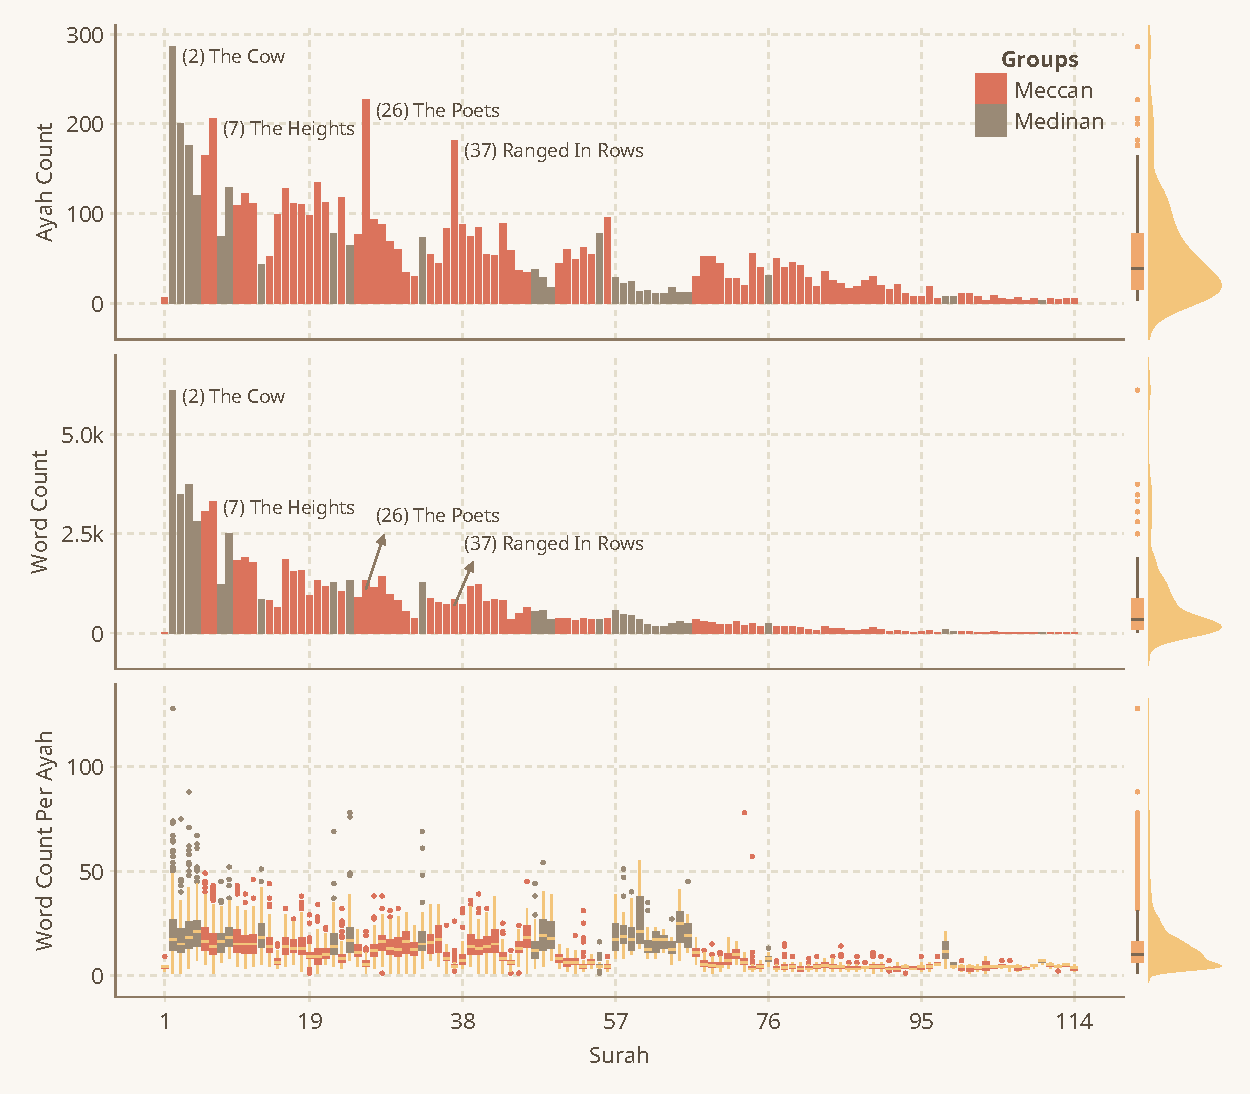
\includegraphics[width=\textwidth]{img/plot1.pdf}
    \caption{Distribution of Meccan and Medinan \arb[trans]{sUwar} \arb{sUwar}}
    \label{fig:result_ayah_word_count}
\end{figure}

Figure \ref{fig:result_ayah_word_count} shows the bar chart of the \arb[trans]{AyAt} \arb{AyAt} counts and word counts, and also the distribution of the word counts and character counts both per \arb[trans]{ayAt} \arb{ayAt}. In this figure, the geographical locations (Meccan or Medinan) of the \arb[trans]{sUraT} \arb{sUraT} based on the \arb[trans]{'asbAb 'alnuzUl} \arb{'asbAb 'alnuzUl} or the 'occasions/circumstances of revelation' are also indicated.

The first obvious pattern, which is known to Muslims, is the monotonically decreasing number of the \arb[trans]{ayAt} \arb{ayAt} after the first \arb[trans]{sUraT} \arb{sUraT}. This is true for both the bar charts of the \arb[trans]{ayAt} \arb{ayAt} count and the word count. An interesting pattern also is that, two \arb[trans]{suwar} \arb{suwar} has significant number of \arb[trans]{AyAt} \arb{AyAt} but with each \arb[trans]{ayAt} \arb{ayAt} having small number of words. These two \arb[trans]{suwar} \arb{suwar} are the \arb[trans]{sUraT} \arb{sUraT} 26th (\arb[trans]{sUraTu 'l-^su`arA'} \arb{sUraTu 'l-^su`arA'} or "the Poet") and 37th (\arb[trans]{sUraTu 'l-.sAffAt} \arb{sUraTu 'l-.sAffAt} or "the Ranged in Rows"), respectively. This can be confirmed even in the Medina Mushaf, where the first page for \arb[trans]{sUraTu 'l-^su`arA'} \arb{sUraTu 'l-^su`arA'} already contains 19 \arb[trans]{AyAt} \arb{AyAt}, and the \arb[trans]{sUraTu 'l-.sAffAt} \arb{sUraTu 'l-.sAffAt} contains 24 \arb[trans]{AyAt} \arb{AyAt} in its first page. This indicates that the said \arb[trans]{suwar} \arb{suwar} contain small number of words per \arb[trans]{ayAt} \arb{ayAt} shown in Figure \ref{fig:result_ayah_word_count}.

Moving on, the distribution of the words per \arb[trans]{ayAt} \arb{ayAt} and the characters per \arb[trans]{ayAt} \arb{ayAt} are shown in the third and fourth rows or plots of Figure \ref{fig:result_ayah_word_count}. It is indeed expected that these distributions are more or less identical, since it is expected that more words means more characters. The reason why the distribution of characters per \arb[trans]{ayAt} \arb{ayAt} is shown is to make it comparable to the work of \citeA{sinai2020oqs}, which will be compared later in Section. 

To interpret these distributions of word count per \arb[trans]{ayAt} \arb{ayAt} and the character count per \arb[trans]{ayAt} \arb{ayAt}, the x-axis is still the 114 \arb[trans]{suwar} \arb{suwar} of the Qur'\=an, while the y-axis is either the count of words (third row plot) per \arb[trans]{ayAt} \arb{ayAt} or the count of characters (fourth row plot) per \arb[trans]{ayAt} \arb{ayAt} in Figure \ref{fig:result_ayah_word_count}. Thus, each boxplot shown in these plots describes the distributions of the count of either the words or characters per \arb[trans]{ayAt} \arb{ayAt}. From these distributions, an interesting groups of distributions at around 57th \arb[trans]{sUraT} \arb{sUraT} to 66th \arb[trans]{sUraT} \arb{sUraT} are observed. These distributions while might be reasoned as easily seen because of its Medinan \arb[trans]{'asbAb 'alnuzUl} \arb{'asbAb 'alnuzUl} color, the mean of these are obviously higher than its surrounding \arb[trans]{sUraT} \arb{sUraT} as seen in the figure. In fact, these \arb[trans]{suwar} \arb{suwar} have lower number of \arb[trans]{ayAt} \arb{ayAt} compared to its surrounding \arb[trans]{suwar} \arb{suwar} (\textit{see} first plot and second plot of Figure \ref{fig:result_ayah_word_count}). Although, the number of words are more or less the same.

Further, it can be observed that the distributions of the Medinan \arb[trans]{suwar} \arb{suwar} tend to have higher mean as opposed to those in Meccan \arb[trans]{suwar} \arb{suwar}, which is indeed the case as seen in later discussions. In fact, as a prelude to this, if the order of the arb[trans]{suwar} \arb{suwar} is based on the \arb[trans]{'asbAb 'alnuzUl} \arb{'asbAb 'alnuzUl}, the observation that Medinan surah has higher number of word or character per \arb[trans]{ayAt} \arb{ayAt} can be seen in Figure \ref{fig:result_ayah_word_count_rev_order}. In this figure, the Medinan \arb[trans]{suwar} \arb{suwar} seen in the latter part of the \arb[trans]{'asbAb 'alnuzUl} \arb{'asbAb 'alnuzUl} clearly have higher mean counts and tend to have variable number of word or character counts per \arb[trans]{ayAt} \arb{ayAt}. This is again true especially when looking at the overall distributions of these categories across \arb[trans]{suwar} \arb{suwar} as in Figure \ref{fig:result_meccan_medinan_dist}.

\begin{figure}[!t]
    \centering
    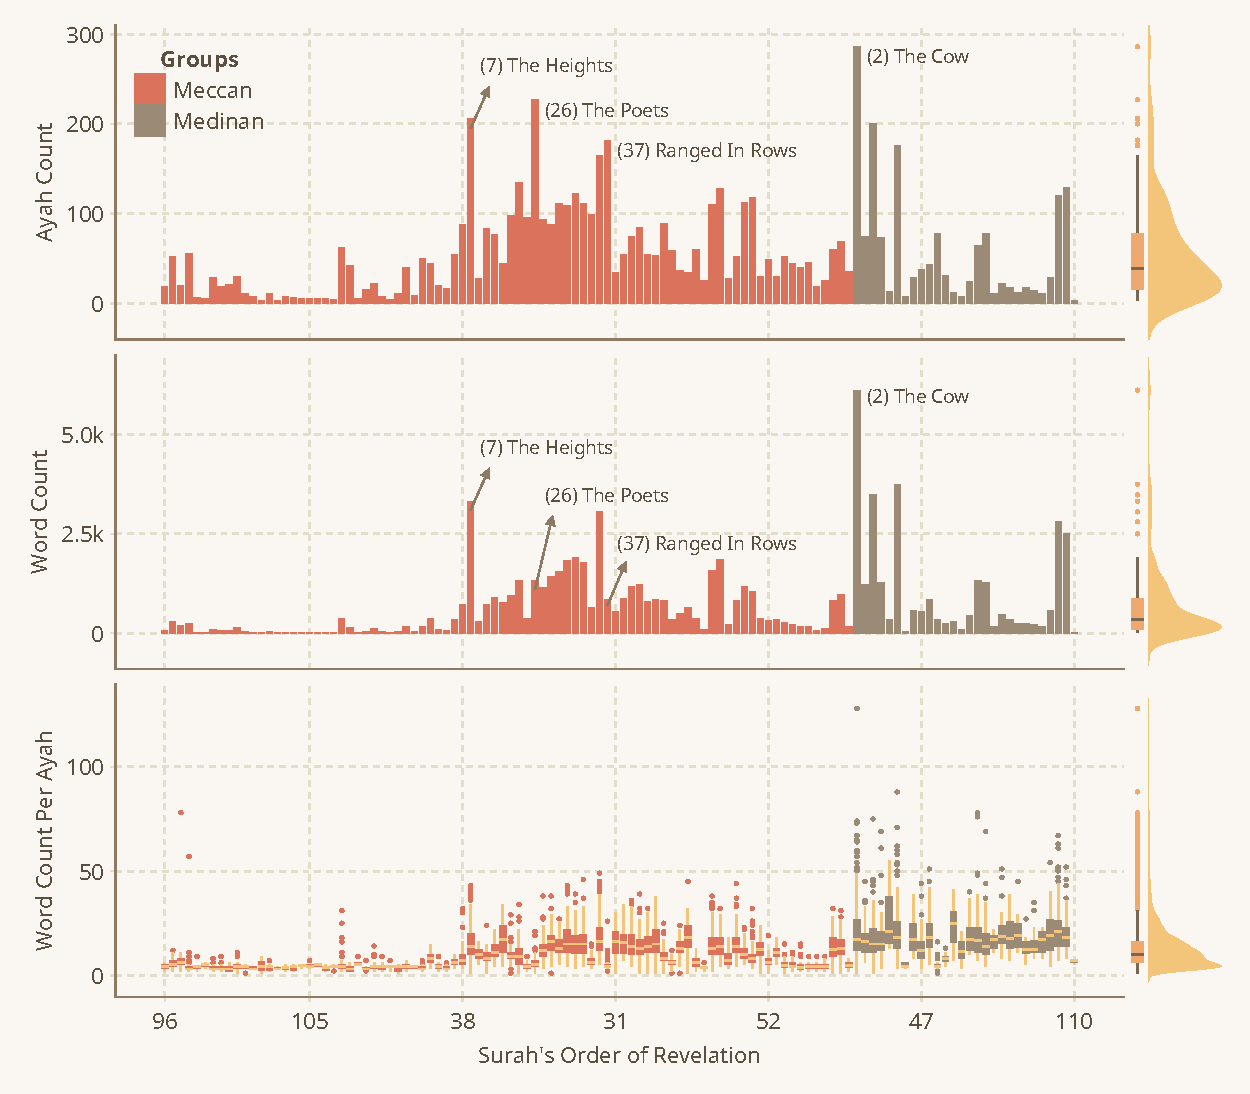
\includegraphics[width=\textwidth]{img/plot2.pdf}
    \caption{Statistics of the words and \arb[trans]{ayAt} \arb{ayAt} (verses) of the Qur'\=an according to revelation order}
    \label{fig:result_ayah_word_count_rev_order}
\end{figure}

\begin{figure}[!t]
    \centering
    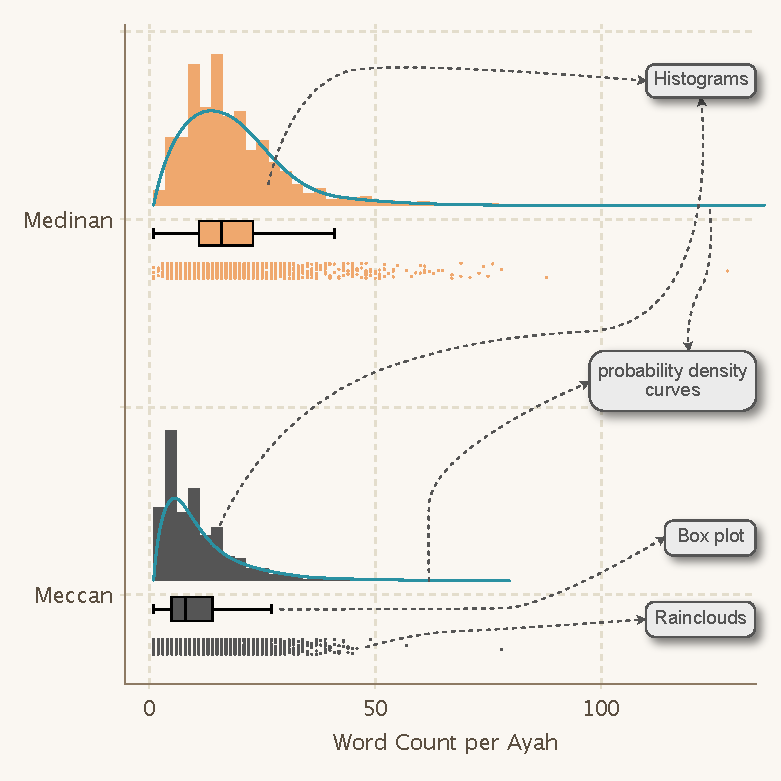
\includegraphics[width=\textwidth]{img/plot3.pdf}
    \caption{Distribution of Meccan and Medinan \arb[trans]{sUwar} \arb{sUwar}}
    \label{fig:result_meccan_medinan_dist}
\end{figure}

\begin{table}
    \caption{Descriptive statistics of the \arb[trans]{ayAt} \arb{ayAt} counts and the counts of its words}
    \label{tbl:desc_stats}
    \begin{tabularx}{\textwidth}[!h]{XXXX}
        \toprule
        Count Data&Mean&Median&Std. Deviation\\
        \midrule
        Ayahs&54.70&39&53.21\\
        Words&679.20&344&931.18\\
        Words per Ayah&10.27&8.23&6.35\\
        \bottomrule
    \end{tabularx}
\end{table}
\subsection{Comparison to Sinai's Inner-Chronology}
The work of \citeA{sinai2020oqs} investigated the same statistical distributions as in the previous section, but has focused from a non-traditionalist view by not basing on the \arb[trans]{'asbAb 'alnuzUl} \arb{'asbAb 'alnuzUl}, and instead mainly on the Qur'\=an's text itself using a transliteration data from Prof. Hans Zirker. The said data is not exactly the same as the one used in here, nor it is publicly verified as the one (Quranic Arabic Corpus and the Tanzil data) used in this study. Nonetheless, if indeed the said transliteration is exactly the same as the one used here once decoded to its Arabic form, the result should more or less be the same. However, while the preprocessing done by \citeA{sinai2020oqs} was not done in the analyses of the previous section, the result of the distributions should not deviate much. In the said study of \citeA{sinai2020oqs}, the findings suggest that there is inner-chronology of the Qur'\=an. This was concluded by the said author by looking at the mean verse length, which is more or less similar to the median verse length indicator used in boxplots of the third and fourth plots of Figures \ref{fig:result_ayah_word_count} and \ref{fig:result_ayah_word_count_rev_order}. Indeed, median is a better metric than mean in this case due to outlier counts seen in the boxplots in Figures \ref{fig:result_ayah_word_count} and \ref{fig:result_ayah_word_count_rev_order}. It is surprising though that he considered those with significant variance or coefficient variations (meaning those \arb[trans]{suwar} \arb{suwar} with very varied number of characters per \arb[trans]{ayAt} \arb{ayAt}) as possible later insertion to the Qur'\=an upon his closer inspection. It may sound polemic to disregard his findings or to attack it, but to be fair to Muslim traditionalists that to believe in such claim requires solid evidence from extant manuscripts and not just from someone's own interpretation of the statistics or literary styles of the \arb[trans]{ayAt} \arb{ayAt}. Indeed, the findings of Prof. Sina's can be categorized as \textit{theories} as it does not have supporting manuscripts that shows one. It may also be difficult to prove so as all Qur'\=anic extant manuscripts are consistent with the current one, including the controversial Sana'a Palimpest, where also Prof. Sinai was fair to admit in his own book \cite{sinai2017} that the said texts have. 

Furthermore, while it is healthy for the advancement of any studies including Qur'\=anic studies to have opposing views. For the case of \citeA{sinai2020oqs}, the premise of not considering \arb[trans]{'asbAb 'alnuzUl} \arb{'asbAb 'alnuzUl} shows a different structure as discussed in the preceding section.
\section{Morphological Analysis}\label{sec:ch4_morphological_analysis}
The second statistical analysis is to analyze the morphological features of the Qur'\=an. There are several ways to do this, and the easiest one is to find a particular word and study its morphologies. This will be the goal of this section, and the important word to study is the name of God in the Qur'\=an and that is \arb[trans]{'l-l_ah} \arb{'l-l_ah}. The root of this word is the \arb[trans]{Alh} \arb[novoc]{Alh}, and thus the morphologies of this root word will be studied and compared againts the \arb[trans]{'asbAb 'alnuzUl} \arb{'asbAb 'alnuzUl} or the 'occasions/circumstances of revelation.' Table \ref{tbl:result_Alh_morphologies} contains the complete list of morphologies of \arb[trans]{Alh} \arb[novoc]{Alh}. The first column in the said table lists the said morphologies, the second column lists its location in \arb[trans]{sUraT} \arb{sUraT} and \arb[trans]{'ayaT} \arb{'ayaT}, the third column lists the total number of \arb[trans]{'ayaT} \arb{'ayaT} that has the said morphology in the Qur'\=an, and the fourth column lists the percentage of \arb[trans]{'ayaT} \arb{'ayaT} whose \arb[trans]{'asbAb 'alnuzUl} \arb{'asbAb 'alnuzUl} is Mecca. The codes on how to generate this table in Julia using QuranTree.jl, Yunir.jl, and DataFrames.jl libraries are shown in Figure \ref{fig:result_Alh_morphologies}.

\begin{table}[!t]
    \begin{tabularx}{\textwidth}[!h]{cXcc}
        \toprule\\[-0.3cm]
        Morph. & Surah \& Ayah & Count & Meccan \% \\[0.2cm]
        \midrule\\[-0.4cm]
        \arb[fullvoc]{'l-l_ahi} & 1:1, 2:8, 2:23, $\cdots$, 104:6, 110:1, 110:2 & $710$ & 47\% \\[0.2cm]
        \arb[fullvoc]{llahi} & 1:2, 2:22, 2:98, $\cdots$, 71:13, 72:18, 82:19 & $122$ & 55\%\\[0.2cm]
        \arb[fullvoc]{'l-l_ahu} & 2:7, 2:10, 2:15, $\cdots$, 98:8, 112:1, 112:2 & $624$ & 39\% \\[0.2cm]
        \arb[fullvoc]{'l-l_aha} & 2:9, 2:26, 2:55, $\cdots$, 72:12, 96:14, 98:5 & $351$ & 30\% \\[0.2cm]
        \arb[fullvoc]{'il---a---_aha} & 2:133, 3:6, 6:106, $\cdots$, 45:23, 47:19, 73:9 & $17$ & 76\% \\[0.2cm]
        \arb[fullvoc]{'il---a---_ahu} & 2:163, 16:22, 18:110, $\cdots$ , 21:108, 29:46, 41:6 & $8$ & 88\% \\[0.2cm]
        \arb[fullvoc]{'il---a---_ahiN} & 3:62, 28:38, 38:65 & $3$ & 67\%\\[0.2cm]
        \arb[fullvoc]{|"'AlihaTaN} & 6:74, 18:15, 21:21, $\cdots$, 36:23, 37:86, 43:45 & $9$ & 100\% \\[0.2cm]
        \arb[fullvoc]{|"'Alihata} & 7:127, 21:36, 21:68, 71:23 & $4$ & 100\% \\[0.2cm]
        \arb[fullvoc]{'il---a---_ahaN} & 7:138, 18:14, 26:29 & $3$ & 100\%\\[0.2cm]
        \arb[fullvoc]{|"'Alihati} & 11:53, 11:54, 19:46, 25:42, 37:36, 37:91, 38:6, 46:22 & $8$ & 100\% \\[0.2cm]
        \arb[fullvoc]{|"'Alihatu} & 11:101 & $1$ & 100\% \\[0.2cm]
        \arb[fullvoc]{'il---a---_ahuN} & 14:52, 21:29, 43:84, 52:43 & $4$ & 100\% \\[0.2cm]
        \arb[fullvoc]{|"'AlihaTuN} & 17:42, 21:22, 21:43 & $3$ & 100\% \\[0.2cm]
        \arb[fullvoc]{'il---a---_ahi} & 20:97, 40:37, 114:3 & $3$ & 100\% \\[0.2cm]
        \arb[fullvoc]{--|"'Alihati}& 21:59, 21:62 & $2$ & 100\%\\[0.2cm]
        \arb[fullvoc]{|"'il---a---_ahuN} & 27:60, 27:61, 27:62, 27:63, 27:64 & $5$ & 100\% \\[0.2cm]
        \arb[fullvoc]{|"'AlihaTa} & 38:5 & $1$ & 100\% \\[0.2cm]
        \arb[fullvoc]{'alihatu} & 43:58 & $1$ & 100\% \\[0.2cm]
        \bottomrule
    \end{tabularx}
    \caption{Morphologies of \arb[novoc]{Alh} in the Qur'\=an}
    \label{tbl:result_Alh_morphologies}
\end{table}

The codes in Figure \ref{fig:result_Alh_morphologies} defines a Julia function called \verb|get_morphologies| from lines 5 to 25. The body of this function contains logics for extracting the morphologies of a given root word. At a high level, the logics has the following flow: it reads the morphological features of the root word \arb[novoc]{Alh}, then it lists down the chapter and verses containing this root word, and then compute the total number of \arb[trans]{AyAt} \arb{AyAt} that contain the given morphology of the given root word. Finally, it returns the output in tabular form that is presented in Table \ref{tbl:result_Alh_morphologies}. The defined \verb|get_morphologies| function can then be used to generate similar tables from other root words without rewriting those codes in lines 5 to 25 of Figure \ref{fig:result_Alh_morphologies}. Indeed, this is the beauty of programming, it can automate the manual process. For example, to generate similar table for the morphology of \arb{r.hm}, the code is as simple as shown in Figure \ref{fig:result_rHm_morphologies}, which shows only the first five morphologies of \arb{r.hm}.

\begin{figure}[!t]
    \centering
    \includegraphics[width=\textwidth]{img/morphologies_Alh.png}
    \caption{Julia code for generating Table \ref{tbl:result_Alh_morphologies}}
    \label{fig:result_Alh_morphologies}
\end{figure}

\begin{figure}[!t]
    \centering
    \includegraphics[width=\textwidth]{img/morphologies_rHm.png}
    \caption{Julia code for generating morphologies of \arb[novoc]{r.hm}}
    \label{fig:result_rHm_morphologies}
\end{figure}

From the result it can be observed that those these morphologies are purely under Meccan: \arb[trans]{'alihatu}  \arb[fullvoc]{'alihatu} - a masculine plural noun in nominative case (\textit{see} Figure \ref{fig:result_mfeat_43_58} for the codes on how to get these details in QuranTree.jl); \arb[trans]{|"'AlihaTa} \arb[fullvoc]{|"'AlihaTa} - a masculine plural noun in accusative case; \arb[trans]{|"'il---a---_ahuN} \arb[fullvoc]{|"'il---a---_ahuN} - a masculine singular noun in indefinite state and nominative case; \arb[trans]{--|"'Alihati} \arb[fullvoc]{--|"'Alihati} - a masculine plural noun in genitive case; \arb[trans]{'il---a---_ahi} \arb[fullvoc]{'il---a---_ahi} - a masculine singular noun in genitive case; \arb[trans]{|"'AlihaTuN} \arb[fullvoc]{|"'AlihaTuN} - a masculine plural noun in indefinite state and nominative case; \arb[trans]{'il---a---_ahuN} \arb[fullvoc]{'il---a---_ahuN} - similar to \arb[trans]{|"'il---a---_ahuN} \arb[fullvoc]{|"'il---a---_ahuN} with slightly different morphology; \arb[trans]{|"'Alihatu} \arb[fullvoc]{|"'Alihatu} - a masculine plural noun in nominative case; \arb[trans]{|"'Alihati} \arb[fullvoc]{|"'Alihati} - a masculine plural noun in genitive case; \arb[trans]{'il---a---_ahaN} \arb[fullvoc]{'il---a---_ahaN} - a masculine singular noun in indefinite state and accusative case; \arb[trans]{|"'Alihata} \arb[fullvoc]{|"'Alihata} - a masculine plural noun in accusative state, \arb[trans]{|"'AlihaTaN} \arb[fullvoc]{|"'AlihaTaN} - a masculine plural noun in indefinite state and accusative case.

\begin{figure}[!t]
    \centering
    \includegraphics[width=\textwidth]{img/mfeat_43_58.png}
    \caption{Julia code for describing morphological features of \arb[trans]{'alihatu} \arb{'alihatu}}
    \label{fig:result_mfeat_43_58}
\end{figure}

The last column in Table \ref{tbl:result_Alh_morphologies} contains the percentages of the Meccan \arb[trans]{AyAt} \arb{AyAt}, therefore among the \arb[trans]{AyAt} \arb{AyAt} that contain the morphologies of \arb[trans]{'l-l_ahi} \arb[fullvoc]{'l-l_ahi} is that 47\% of those are Meccan. This column was generated by the code in Figure \ref{fig:result_meccan_ratio}.

\begin{figure}[!t]
    \centering
    \includegraphics[width=\textwidth]{img/meccan_ratio.png}
    \caption{Julia code for generating last column of Table \ref{tbl:result_meccan_ratio}}
    \label{fig:result_meccan_ratio}
\end{figure}

Sample \arb[trans]{AyAt} \arb{AyAt} are given for Q43:59, Q21:59, and Q2:23. The first \arb[trans]{'ayaT} \arb{'ayaT} contains the only morphology for \arb[trans]{'alihatu} \arb[fullvoc]{'alihatu} in the Qur'\=an, which is highlighted in red. The context of this \arb[trans]{'ayaT} \arb{'ayaT} is that it the \textit{gods} (\arb[trans]{'alihatu} \arb[fullvoc]{'alihatu}) referred here are the dieties worshipped by the disbelievers. The one they cited here as \textit{him} is given in the previous  \arb[trans]{'ayaT} \arb{'ayaT} as Jesus \txarb{\fontspec{Scheherazade New} ﵇}, the son of Mary \txarb{\fontspec{Scheherazade New} ﵍}. 

\begin{bottomtitledframe}{Q43:58}
    \begin{center}
        \begin{arab}[fullvoc]
            min ((sUraTu 'l-zuxrufi)): waqAlUA |"'a\arbcolor[red]{'a_alihatu}nA xayruN 'am huwa mA .darabUhu laka 'illA jadalA bal hum qawmun xA.simUn
        \end{arab}
        \begin{arab}[trans]
            min ((sUraTu 'l-zuxrufi)): waqAlUA |"'a\arbcolor[red]{'a_alihatu}nA xayruN 'am huwa mA .darabUhu laka 'illA jadalA bal hum qawmun xA.simUn
        \end{arab}
    \end{center}
    From Surah \textit{Ornaments of Gold}: saying, 'Are our \textcolor{red}{gods} better or him?' --- they cite him only to challenge you: they are a contentious people ---
\end{bottomtitledframe}

The next Meccan \arb[trans]{'ayaT} \arb{'ayaT} is Q21:59, which contain the morphology for \arb[trans]{--|"'Alihati} \arb[fullvoc]{--|"'Alihati}, which refers to \textit{gods} or \textit{deities} of the disbelievers. In this \arb[trans]{'ayaT} \arb{'ayaT} the question is coming from disbelievers during the time of Abraham \txarb{\fontspec{Scheherazade New} ﵇}, after he destroyed the idols worshipped by his father and the disbelievers. Indeed, the not so common morphologies for \arb[novoc]{alh} refer to false gods and dieties and not to the true God that the Qur'\=an refers to. 

\begin{bottomtitledframe}{Q21:59}
    \begin{center}
        \begin{arab}[fullvoc]
            min ((sUraTu 'l-'anbiyA'i)): waqAlUA man fa`ala ha_a_dA bi\arbcolor[red]{--|"'Alihati}n'A 'innahu lamina 'l-.za_alimIna
        \end{arab}
        \begin{arab}[trans]
            min ((sUraTu 'l-'anbiyA'i)): waqAlUA man fa`ala ha_a_dA bi\arbcolor[red]{--|"'Alihati}n'A 'innahu lamina 'l-.za_alimIna
        \end{arab}
    \end{center}
    From Surah \textit{The Prophets}: They said, 'Who has done this to our \textcolor{red}{gods}? How wicket he must be!
\end{bottomtitledframe}

Finally, the example for the use of \arb[novoc]{alh} morphology to refer to the true God in the Qur'\=an is given in Q2:23, for \arb[trans]{'l-lahi} \arb[fullvoc]{'l-lahi}. Here the context is the challenge of Allah or God to the disbelievers to produce a single \textit{s\=urah} \arb{sUraT} or chapter like that in the Qur'\=an. This is indeed a challenge that is still valid until today, and no one has ever produced a single \textit{s\=urah} \arb{sUraT} like the Qur'\=an. If there was one, it should have been published in a reputable journal addressing this challenge. The problem with producing this is that it should be with the same eloquence and beauty of the Qur'\=an. This is indeed a challenge that is still valid until today, and no one has ever produced a single \textit{s\=urah} \arb{sUraT} like the Qur'\=an. This is part of the \arb[trans]{'al-'i`jAzu 'l-qur`an} \arb{'al-'i`jAzu 'l-qur`an} or \textit{the inimitability of the Qur'\=an}, which is one of the main reasons why the Qur'\=an is considered to be a miracle by the Muslims.

\begin{bottomtitledframe}{Q2:23}
    \begin{center}
        \begin{arab}[fullvoc]
            min ((sUraTu 'l-baqaraTi)): wa-'in kuntum fI raybiN mmimmA nazzalnA `alY_a `abdinA fa'tUA bisUraTiN mmin mmi_tlihi wa-"ad`UA ^suhada'A'akum mmin dUni \arbcolor[red]{'l-lahi} 'in kuntum .sa--_a--diqIna
        \end{arab}
        \begin{arab}[trans]
            min ((sUraTu 'l-baqaraTi)): wa-'in kuntum fI raybiN mmimmA nazzalnA `alY_a `abdinA fa'tUA bisUraTiN mmin mmi_tlihi wa-"ad`UA ^suhada'A'akum mmin dUni \arbcolor[red]{'l-lahi} 'in kuntum .sa--_a--diqIna
        \end{arab}
    \end{center}
    From Surah \textit{The Cow}: If you have doubts about the revelation We have sent down to Our servant, then produce a single surah like it --- enlist whatever supporters you have other than \textcolor{red}{God} --- if you truly [think you can].
\end{bottomtitledframe}

The results shown in Table \ref{tbl:result_Alh_morphologies} found several verses for the common morphologies of \arb[novoc]{alh}, while those rare ones have been found by the codes in Figure \ref{fig:result_Alh_morphologies}. In fact, the whole results in Table \ref{tbl:result_Alh_morphologies} were generated in under 5 seconds and few lines of codes from Figure \ref{fig:result_Alh_morphologies} and \ref{fig:result_meccan_ratio}. Had it been done manually, it would have taken days, weeks or even months. Plus the final results will likely have human errors, or at least it will need another person to verify the results, which too will take time. This is the main advantage of programming as it can automate such process with great accuracy, so long as the codes are accurate. Generating new morphologies for any given root can be done in just one line of code as in the first line of code in Figure \ref{fig:result_rHm_morphologies}.

% \begin{bottomtitledframe}{Q43:58}
%    Hello!
% \end{bottomtitledframe}



\section{Thematic Analysis}\label{sec:result_thematic_analysis}
From previous section, it was concluded that those morphologies that are unique to Meccan \arb[trans]{sUwar} \arb{sUwar} are considered to refer to false gods or deities worshipped by the disbelievers. Whereas those with common morphologies are considered to refer to the true God. Sample \arb[trans]{sUwar} \arb{sUwar} were given above for three \arb[trans]{ayaT} \arb{ayaT}, but it would be better to also understand the themes of \arb[trans]{AyAt} \arb{AyAt} for other morphologies, especially those that are common. However, doing this manually would be very tedious and time consuming, since the first morphology, \arb[trans]{'l-lahi} \arb[fullvoc]{'l-lahi}, contain 710 \arb[trans]{AyAt} \arb{AyAt}. Trying to summarize this manually would take so much time, and will also be prone to human error. How to automate then?

In Statistics and Machine Learning, there are techniques to do this mathematically. Among the basic method is what is called Latent Dirichlet Allocation (LDA), an algorithm that can produce keywords as topics from a given text. The algorithm is based on the idea that each document is a mixture of topics, and each topic is a mixture of words. The algorithm works by assigning each word in the document to a topic, and then updating the topic assignments based on the words assigned to each topic. This process is repeated until the topic assignments converge. The result is a set of topics, each represented by a set of words, that can be used to summarize the document. LDA has been effective for topic modeling and has been widely used in various applications, including text classification, information retrieval, and document clustering.

Another approach to topic modeling is using the BERT (Bidirectional Encoder Representations from Transformers) model, in layman's term, it is an artificial intelligence model that can understand the meaning of words in a sentence by looking at the context of the words around it. The idea is that BERT can generate a numerical representation of a word or a sentence, which can then be used to find similar words or sentences. Since it can be used to find similar words, it therefore can be used to find themes --- which groups similar words. This concept is called BERTopic. 

The third approach to topic modeling or thematic clustering is to use Generative Pre-trained Transformer (GPT) model. The idea is that GPT can generate a summary of a given text, and this summary can be used to find the themes of the text. This approach is similar to LDA, but it uses a different algorithm to generate the summary. The advantage of using GPT is that it can generate a more accurate summary than LDA, and it can also be used to generate summaries for longer texts. For many readers, ChatGPT is the most popular AI model. Indeed, this is the GPT model referred here. 

Among the three approaches mentioned, the third one is the best for the study as it can do everything the first two approaches do, but with human-readable summary and many GPT models have been trained on Qur'\=an data. There are many open-sourced GPT models that can be used, but those commercialized one are more accurate, such as the ChatGPT or the ClaudeAI. For this study, Claude 3.7 Sonnet GPT model is used.

\begin{listing2}[!t]
    \centering
    \includegraphics[width=\textwidth]{img/ayah_morph_extract.png}
    \caption{Julia code for generating last column of Table \ref{tbl:result_meccan_ratio}}
    \label{fig:result_thematic_analysis}
\end{listing2}

\begin{table}[!h]
    \begin{tabularx}{\textwidth}[!h]{cXcc}
        \toprule\\[-0.3cm]
        Morph. & Surah \& Ayah & Count & Meccan \% \\[0.2cm]
        \midrule\\[-0.4cm]
        \arb[fullvoc]{'l-l_ahi} & Divine Unity \& Singularity (Tawhid) [6:164, 28:88, 2:163]; Faith \& Belief (Iman) [49:15, 65:11]; Divine Guidance \& Revelation [2:2, 5:48]; Prophet \& Messengers [2:136, 48:29]; The Day of Judgement \& Afterlife [2:281, 68:34]; Moral \& Ethical Teachings [16:90, 5:1]; Stories of Previous Nations [47:10]; Relationship Between Allah \& Creation [50:16, 51:56]; Rules \& Legislation [62:9, 4:2]; Struggle \& Perseverance [22:78, 2:155] & $710$ & 47\% \\[0.2cm]
        \arb[fullvoc]{llahi} & Divine Sovereignty \& Ownership [2:284, 3:109, 3:129]; Divine Attributes [4:170, 31:26, 4:139, 9:91]; Creator \& Sustainer [6:1, 35:1]; Purpose of Worship [53:62, 22:31]; Divine Judgement \& Authority [22:56, 24:64, 3:129]; Gratitude \& Praise [1:2, 6:1, 34:1, 35:1]; Divine Will \& Power [14:4, 3:129]; Submission to Allah [2:112, 4:125] & $122$ & 55\%\\[0.2cm]
        \arb[fullvoc]{'l-l_ahu} & Divine Unity \& Singularity (Tawhid) [112:1, 2:255, 2:116, 10:68]; Divine Sovereignty \& Power [7:54, 10:3]; Divine Knowledge [3:29, 9:94]; Divine Justice [40:20, 3:57]; Divine Guidance [2:213, 24:46, 57:25]; Divine Will \& Decree [14:27, 5:48]; Divine Names \& Attributes [59:24, 24:35]; Relationship with Believers [98:8]; Divine Creation \& Sustenance [23:14, 7:54]  & $624$ & 39\% \\[0.2cm]
        \arb[fullvoc]{'l-l_aha} & Divine Unity \& Singularity (Tawhid) [7:59, 19:36, 98:5]; Divine Attributes [49:16, 9:5, 2:284]; Obedience to Allah \& His Messenger [4:59, 64:12, 48:17]; Piety \& God Conciousness [3:102, 2:194, 8:25]; Reward \& Punishment [47:12, 40:17, 22:14]; Prayer, Charity, \& Righteous Deeds [98:5]; Stories of Prophets \& Past Nations [11:50, 11:61]; Faith \& Belief [49:10]; Justice \& Fairness [16:90] & $351$ & 30\% \\[0.2cm]
        \arb[fullvoc]{'il---a---_aha} & 2:133, 3:6, 6:106, $\cdots$, 45:23, 47:19, 73:9 & $17$ & 76\% \\[0.2cm]
        \arb[fullvoc]{'il---a---_ahu} & 2:163, 16:22, 18:110, $\cdots$ , 21:108, 29:46, 41:6 & $8$ & 88\% \\[0.2cm]
        \arb[fullvoc]{'il---a---_ahiN} & 3:62, 28:38, 38:65 & $3$ & 67\%\\[0.2cm]
        \arb[fullvoc]{|"'AlihaTaN} & 6:74, 18:15, 21:21, $\cdots$, 36:23, 37:86, 43:45 & $9$ & 100\% \\[0.2cm]
        \arb[fullvoc]{|"'Alihata} & 7:127, 21:36, 21:68, 71:23 & $4$ & 100\% \\[0.2cm]
        \arb[fullvoc]{'il---a---_ahaN} & 7:138, 18:14, 26:29 & $3$ & 100\%\\[0.2cm]
        \arb[fullvoc]{|"'Alihati} & 11:53, 11:54, 19:46, 25:42, 37:36, 37:91, 38:6, 46:22 & $8$ & 100\% \\[0.2cm]
        \arb[fullvoc]{|"'Alihatu} & 11:101 & $1$ & 100\% \\[0.2cm]
        \arb[fullvoc]{'il---a---_ahuN} & 14:52, 21:29, 43:84, 52:43 & $4$ & 100\% \\[0.2cm]
        \arb[fullvoc]{|"'AlihaTuN} & 17:42, 21:22, 21:43 & $3$ & 100\% \\[0.2cm]
        \arb[fullvoc]{'il---a---_ahi} & 20:97, 40:37, 114:3 & $3$ & 100\% \\[0.2cm]
        \arb[fullvoc]{--|"'Alihati}& 21:59, 21:62 & $2$ & 100\%\\[0.2cm]
        \arb[fullvoc]{|"'il---a---_ahuN} & 27:60, 27:61, 27:62, 27:63, 27:64 & $5$ & 100\% \\[0.2cm]
        \arb[fullvoc]{|"'AlihaTa} & 38:5 & $1$ & 100\% \\[0.2cm]
        \arb[fullvoc]{'alihatu} & 43:58 & $1$ & 100\% \\[0.2cm]
        \bottomrule
    \end{tabularx}
    \caption{Morphologies of \arb[novoc]{Alh} in the Qur'\=an}
    \label{tbl:result_Alh_morphologies_theme}
\end{table}

\section{Rhythmic Analysis}\label{sec:result_rhythmic_analysis}
\section{Theory of Concentric Structure}
One of the specific items for the second objective of this paper is on the theory of concentrism, and how can this be formulated statistically, and what are the insights that can be extracted. The idea of the theory of concentrism is that a given texts with define partition follows a ring or concentric structure, which is a literary form where the text is organized in such a way that it mirrors itself around a central point. This means that the beginning and ending sections correspond to each other, moving inward until the center of the text, which often contains the main message or theme. This particular pattern was observed by linguistic experts that it got documented in a book by \citeA{farrin2014structure}. This theory can be defined mathematically as follows:

\begin{defn}[\it Concentric]\label{defn:concentric}
    Let $\mathscr{D}$ be a collection of texts, then $\mathscr{D}$ is said to have a \textit{concentric} or \textit{ring} structure if and only if $\exists\;\mathscr{A}_i\subseteq\mathscr{D},\mathscr{C}\subseteq\mathscr{D},$ and $\mathscr{A}_i^{*}\subseteq\mathscr{D},i\in\mathbb{N}_1$; and that these sets are arranged as follows in $\mathscr{D}$:  $\mathscr{A}_1,\cdots,\mathscr{A}_n,\mathscr{C},\mathscr{A}_1^{*},\cdots,\mathscr{A}_n^{*}$, such that $\mathscr{A}_i^{*}$ \underline{mirrors} $\mathscr{A}_i$ in semantic, and that $\mathscr{C}$ is the center texts of the document $\mathscr{D}$ that is \underline{not related} to both $\mathscr{A}_i$ and $\mathscr{A}_i^{*}$.
\end{defn}

The underlined words above will be used in the next section, because mathematically it begs further definition on what we mean by "mirrors" and "not related" mathematically. This will be defined in the next section. Now, another pattern that was observed by \citeA{farrin2014structure} as chiasmus, which is basically \textit{ring} structure but the second half of the ring after the center is the "complement" or "reversal" of the first half of the document before the center. The following is its mathematical definition.

\begin{defn}[\it Chiasmus]\label{defn:chiasmus}
    Let $\mathscr{D}$ be a collection of texts, then $\mathscr{D}$ is said to have a \textit{concentric} or \textit{ring} structure if and only if $\exists\;\mathscr{A}_i\subseteq\mathscr{D},\mathscr{C}\subseteq\mathscr{D},$ and $\mathscr{A}_i^{*}\subseteq\mathscr{D},i\in\mathbb{N}_{geq 1}$; and that these sets are arranged as follows in $\mathscr{D}$:  $\mathscr{A}_1,\cdots,\mathscr{A}_n,\mathscr{C},\mathscr{A}_1^{c},\cdots,\mathscr{A}_n^{c}$, such that $\mathscr{A}_i^{c}$ is the \underline{complement} or \underline{reversal} of $\mathscr{A}_i$ in semantic, and that $\mathscr{C}$ is the center texts of the document $\mathscr{D}$ that is \underline{not related} to both $\mathscr{A}_i$ and $\mathscr{A}_i^{c}$.
\end{defn}
There are other structures that can be observed in the Qur'\=an, like \textit{parallelism} where themes are repeated in other \arb[trans]{sUraT} \arb{sUraT}; and \textit{segment structure}, where a particular segment starts and ends with similar phrases or themes, creating a bracket around the content; but, these other structures are not studied in this paper. Apart from this, there is also the "mathematical patterns" of the Qur'\=an which has been extensively studied by \citeA{rashad1981}, but this is also not studied in this paper.
\subsection{Bayesian Optimization}\label{sec:bayes-opt}
From Defn. \ref{defn:concentric} and \ref{defn:chiasmus}, it both states that, a document $\mathscr{D}$ may only be considered \textit{concentric} or \textit{chiasmus} if and only if "there exist", denoted by the symbol $\exists$. Indeed, subset of texts $\mathscr{A}_i$s, $\mathscr{C}$, and $\mathscr{A}_i^{*}$ or $\mathscr{A}_i^{\text{c}}$ are all determined manually by the investigator. In this study, we propose to automate the determination of these subsets of texts of document $\mathscr{D}$, and this is through the use of an optimization algorithm called Bayesian Optimization. The idea behind Bayesian optimization is that it approximates the objective function with a \textit{surrogate} function, and using this surrogate to find the global maximum or minimum of the objective function. Furthermore, it does this by fitting the surrogate function to the objective function in as few input points or iteration as possible. As such, an \textit{acquisition} function is needed for choosing smartly the next input points to be used for fitting the surrogate. Using these components, a Bayes' Theorem is used in fitting the surrogate.

To do this, a \textit{global objective function} must be defined, for this study, the cosine similarity discussed in the previous section will be used as the said cost function that will either be maximized or minimized. The core model for this optimization is the Gaussian Process defined below.
\subsubsection{Surrogate Function}
The surrogate function aims to approximate the objective function. In Bayesian, optimization, the surrogate function is defined by the Gaussian process (GP).
\begin{defn}[\it Gaussian Process]\label{defn:gp}
    Let $Y_1,Y_2,\cdots,Y_T$ be sequence of random variables such that $Y_t\in\mathbf{Y}$, then the sequence is a \textit{Gaussian process} (GP) if and only if $\mathbf{Y}\overset{\mathrm{iid}}{\sim}\mathcal{N}(\boldsymbol{\mu}, \boldsymbol{\Sigma})$.
\end{defn}
\begin{defn}[\it Parameter Space]\label{defn:parameter_space}
    Let $\mathbf{s}_i\in\mathscr{D}$ be a word embedding of an \arb[trans]{'ayaT} \arb{'ayaT} in document $\mathscr{D}$, which can be a \arb[trans]{sUraT} \arb{sUraT}, group of \arb[trans]{suwar} \arb{suwar}, or group of \arb[trans]{'Ayat} \arb{'Ayat} within a \arb[trans]{sUraT} \arb{sUraT}. Further, suppose $\mathscr{A}_i,\mathscr{C},\mathscr{A}_i^{*}\subseteq\mathscr{D}$ such that $\mathscr{A}_i:=\{\mathbf{s}_{i,1},\cdots,\mathbf{s}_{i,n}\},\linebreak\mathscr{C}:=\{\mathbf{s}_{n+1},\cdots,\mathbf{s}_{n+c}\}$, and $\mathscr{A}_i^{*}:=\{\mathbf{s}_{i,(n+c+1)},\cdots,\mathbf{s}_{i,(n+c+n)}\}$, then the \textit{parameters} to be optimized are assigned to $\mathbf{v}:=[n,c]^{\text{T}}$, and since $n,c,m\in\mathbb{N}_{\geq 2}$, then the \textit{parameter space} is $\mathscr{P}:=\mathbb{N}_{\geq 2}\times\mathbb{N}_{\geq 2}\times\mathbb{N}_{\geq 2}=(\mathbb{N}_{\geq 2})^3$, so that $\mathbf{v}\in\mathscr{P}$. 
\end{defn}
\begin{defn}[\it Semi-Circle Cost Function]\label{defn:semi_circle_cost}
    From Defn. \ref{defn:parameter_space}, let $r_1$ to denote that $\mathscr{A}_i$ is "related" to $\mathscr{A}_i^{*}$, and $r_2$ to denote that $\mathscr{A}_i$ is "reversal" of $\mathscr{A}_i^{*}$, such that $\eta:=\{r_1,r_2\}$, then  the \textit{semi-circle} cost function between $\mathscr{A}_i$ and $\mathscr{A}_i^{*}$ is defined as:
    \begin{equation}
        \operatorname{\gamma}_{a}(\mathbf{v};\mathscr{A}_i,\mathscr{A}_i^{*},\eta):=\begin{cases}
            \frac{1}{n}\sum_{k=1}^{n}\cos\left(\theta_{\mathbf{s}_{i,k};\mathbf{s}_{i,n+l}}\right),&\text{if}\;\eta=r_1\\
            1-\frac{1}{n}\sum_{k=1}^{n}\cos\left(\theta_{\mathbf{s}_{i,k};\mathbf{s}_{i,n+l}}\right),&\text{if}\;\eta=r_2\\
        \end{cases}
    \end{equation}
\end{defn}
\begin{defn}[\it Center Cost Function]\label{defn:center_cost}
    From Defn. \ref{defn:parameter_space}, the \textit{center} cost function is defined as:
    \begin{equation}
        \operatorname{\gamma}_{b}(\mathbf{v};\mathscr{A}_i,\mathscr{C},\mathscr{A}_i^{*}):=2-\frac{1}{nc}\sum_{k=1}^{n}\sum_{l=1}^{c}\cos\left(\theta_{\mathbf{s}_{i,k};\mathbf{s}_{n+l}}\right)-\frac{1}{nc}\sum_{k=1}^{n}\sum_{l=1}^{c}\cos\left(\theta_{\mathbf{s}_{n+l};\mathbf{s}_{i,n+c+k}^{*}}\right).
    \end{equation}
\end{defn}
\begin{defn}[\it Global Cost Function]\label{defn:global_cost}
    From Defn. \ref{defn:parameter_space}-\ref{defn:center_cost}, the \textit{global} cost function is defined as:
    \begin{equation}
        \operatorname{\gamma}_{g}(\mathbf{v};\mathscr{A}_i,\mathscr{C},\mathscr{A}_i^{*},\eta):=\operatorname{\gamma}_{a}(\mathbf{v};\mathscr{A}_i,\mathscr{A}_i^{*},\eta)+\operatorname{\gamma}_{b}(\mathbf{v};\mathscr{A}_i,\mathscr{C},\mathscr{A}_i^{*})
    \end{equation}
\end{defn}
\begin{defn}[\it Optimal Parameters] From Defn. \ref{defn:global_cost}, the optimal parameters would be:
\begin{equation}
    \hat{\mathbf{v}}:=\underset{n,c}{\arg\min}\operatorname{\gamma}_{g}(\mathbf{v};\mathscr{A}_i,\mathscr{C},\mathscr{A}_i^{*},\eta),
\end{equation}    
\end{defn}
\begin{prop}\label{prop:hypedist}
    Let $\mathscr{P}$ be the parameter space and suppose $\gamma(\mathbf{v})\overset{\mathrm{iid}}{\sim}\mathcal{N}(m(\mathbf{v}),k(\mathbf{v},\mathbf{v})), \linebreak\forall \mathbf{v}\in\mathscr{P}$, then for any $\boldsymbol{\delta}:=[\gamma(\mathbf{v}_1),\cdots,\gamma(\mathbf{v}_n)]^{\top}$, $\boldsymbol{\delta}\overset{\mathrm{iid}}{\sim}\mathcal{N}_n(\mathbf{m},\mathbf{K})$, where 
    \begin{equation}
        \mathbf{m}:=[m(\mathbf{v}_1),\cdots,m(\mathbf{v}_n)]^{\top}
    \end{equation}
    and
    \begin{equation}
        \mathbf{K}:=\left[\begin{matrix}
        k(\mathbf{v}_1,\mathbf{v}_1)&\cdots&k(\mathbf{v}_1,\mathbf{v}_n)\\
        \vdots&\ddots&\vdots\\
        k(\mathbf{v}_n,\mathbf{v}_1)&\cdots&k(\mathbf{v}_n,\mathbf{v}_n)\\
        \end{matrix}\right]
    \end{equation}
\end{prop}
\begin{proof}
    The proof follows from the proof of Theorem 1.2.9 of \citeA{muirhead2005}.
\end{proof}
\begin{remark}
    From Proposition \ref{prop:hypedist} and Definition \ref{defn:gp}, $\boldsymbol{\delta}$ is a GP.
\end{remark}
\begin{prop}\label{prop:jointpdf}
    From Proposition \ref{prop:hypedist}, suppose $\boldsymbol{\delta}_{*}:=[\gamma(\mathbf{v}_{n+1}),\cdots,\gamma(\mathbf{v}_{n+p})]^{\top}$, such that $\boldsymbol{\delta}_{*}\overset{\mathrm{iid}}{\sim}\mathcal{N}_p(\mathbf{m}_*,\mathbf{K}_*)$ then 
    \begin{equation}
        \left[
        \begin{matrix}
            \boldsymbol{\delta}\\
            \boldsymbol{\delta}_{*}\\
        \end{matrix}
        \right]\overset{\mathrm{iid}}{\sim}
        \mathcal{N}_{n+p}\left(\left[
        \begin{matrix}
            \mathbf{m}\\
            \mathbf{m}_{*}\\
        \end{matrix}
        \right],\left[
        \begin{matrix}
            \mathbf{K}&\mathbf{K}_{*}\\
            \mathbf{K}_{*}^{\top}&\mathbf{K}_{**}\\
        \end{matrix}
        \right]\right)
    \end{equation}
\end{prop}
\begin{proof}
    Let $\mathbf{u}:=[\boldsymbol{\delta},\boldsymbol{\delta}_{*}]^{\top}$, then $\mathbf{u}=[\gamma(\mathbf{v}_1),\cdots,\gamma(\mathbf{v}_{n+p})]^{\top}$. Further, since $\mathbf{\gamma}(\mathbf{v}_i)\overset{\mathrm{iid}}{\sim}\mathcal{N}(m(\mathbf{v}_i),k(\mathbf{v}_i,\mathbf{v}_i)),\forall i\in\mathbb{N}_{\leq n+p}$, then the joint distribution of the $\gamma(\mathbf{v}_i)$s, i.e. $\mathrm{Pr}(\mathbf{u})$, follows from the proof of Theorem 1.2.9 of \citeA{muirhead2005}.
\end{proof}
\begin{cor}\label{cor:condpdf}
From Proposition \ref{prop:jointpdf}, let $\mathbf{m}$ and $\mathbf{m}_{*}$ be zero vectors, then the following conditional distribution is true:
    \begin{equation}\label{eq:gp_updater}    \boldsymbol{\delta}_*\mid\boldsymbol{\delta}\overset{\mathrm{iid}}{\sim}\mathcal{N}_{p}(\mathbf{K}_{*}^{\top}\mathbf{K}^{-1}\boldsymbol{\delta},\mathbf{K}_{**}-\mathbf{K}_{*}^{\top}\mathbf{K}^{-1}\mathbf{K}_{*}).
\end{equation}
\end{cor}
\begin{proof}
    The proof follows by reversing the condition from $\mathbf{X}_1\mid\mathbf{X}_2$ to $\mathbf{X}_2\mid\mathbf{X}_1$ of the proof of Theorem 1.2.11 of \cite{muirhead2005}.
\end{proof}
\begin{defn}[\it Lower Confidence Bound]\label{defn:lcb}
    Let $m(\mathbf{v})$ be the mean of the GP, then the Lower Confidence Bound (LCB) notated as $\xi$ is given by
    \begin{equation}
        \xi(\mathbf{v}\mid\zeta):=m(\mathbf{v})-\zeta k(\mathbf{v},\mathbf{v}),
    \end{equation}
    where $\zeta$ is the balancing factor.
\end{defn}
The \textit{global cost} computed from the global cost function in Defn. \ref{defn:global_cost} is approximated by the Gaussian process (the surrogate function) defined in Defn. \ref{defn:gp} through Proposition \ref{prop:hypedist}. So that, for any new observed global cost computed from the new parameter input $\mathbf{v}$, chosen by the acquisition function defined in Defn. \ref{defn:lcb}, the joint distribution with the previous global cost is given in Proposition \ref{prop:jointpdf}. Therefore, computing for the conditional distribution of the new global costs conditioned on previous global cost is given in Corollary \ref{cor:condpdf}. The process of acquiring new parameter candidate and computing the global cost is done iteratively. The algorithm converges until there is no significant changes on the new parameter candidate relative to the preceding parameter candidate, or alternatively, until a specified maximum iteration.
\begin{center}
    \textcolor{red}{add theoretical Bayes theorem computations here}
\end{center}
\subsection{Discussions on Islamic Philosophy of Qur'\=an's Structural Analysis}
\newpage
\section{Topic Modeling}\label{sec:ch4_topic_modeling_result}
\subsection{Latent Dirichlet Allocation}
\subsection{Bidirectional Encoder Representation from Transformer}
\subsection{Generative Pre-Trained Transformer}
\section{Relating to other Islamic Texts and Analyses}\label{sec:ch4_relating_islamic_texts}
\subsection{Retrieval-Augmented Generation Approach}
\section{Limitations of the Models}

\section{Advantages of Computation}

\chapter{Future Research}\label{ch:future_research}
\begin{itemize}
    \item Change in rhythmic style mean change in topic?
    \item Superimposition of the morphological features to rhythmic patterns to get a resultant signature
\end{itemize}
\bibliographystyle{apacite}
\bibliography{reference}
\appendix
\chapter{Theoretical Results}
\label{appendix:theoretical_results}
\setcounter{section}{1}
The following are the mathematical formulations of the proposed solution for finding the optimal structural borders of classes of concentric structure.
\begin{defn}[\it Concentric]\label{defn:concentric}
    Let $\mathscr{D}$ be a collection of texts, then $\mathscr{D}$ is said to have a \textit{concentric} or \textit{ring} structure if and only if $\exists\;\mathscr{A}_i\subseteq\mathscr{D},\mathscr{C}\subseteq\mathscr{D},$ and $\mathscr{A}_i^{*}\subseteq\mathscr{D},i\in\mathbb{N}_1$; and that these sets are arranged as follows in $\mathscr{D}$:  $\mathscr{A}_1,\cdots,\mathscr{A}_n,\mathscr{C},\mathscr{A}_1^{*},\cdots,\mathscr{A}_n^{*}$, s.t. $\mathscr{A}_i^{*}$ \underline{mirrors} $\mathscr{A}_i$ in semantic, and that $\mathscr{C}$ is the center section of the document $\mathscr{D}$ that is \underline{not related} to both $\mathscr{A}_i$ and $\mathscr{A}_i^{*}$.
\end{defn}

The underlined words above will be used in the next section, because mathematically it begs further definition on what we mean by "mirrors" and "not related." This will be defined in the next section. Now, another pattern that was observed by \citeA{farrin2014structure} is \textit{chiasm}, which is basically \textit{concentrism} structure but with no center class. Succeeding definitions and results outline the proposed mathematical formulation of finding the optimal structural borders of a given number of classes of concentric structure.
\begin{defn}[\it CL-AraBERT Embedding Function]
    Let $\mathscr{D}$ be the collection of texts, e.g. \arb[trans]{'AyAt} \arb{'AyAt} in a \arb[trans]{suwar} \arb{suwar}, and let $s_i\in\mathscr{D}$, then  $\omega:s\rightarrow\mathbb{R}^{r},r\in\mathbb{N}_{\geq 1}$ is the \textit{CL-AraBERT} embedding function s.t. $\omega(s_i)=\mathbf{z}_i\in\mathbb{R}^{r}$, where $\mathbf{z}_i$ is the $i$th CL-AraBERT sentence embedding of the document $\mathscr{D}$, and $r$ is the dimension of the embedding space. 
\end{defn}
\begin{defn}[\it Structural Borders]\label{defn:structural_borders}
    Let $\mathscr{D}$ be a collection of texts, then for $s_i\in\mathscr{D}, i\in\mathbb{N}$, \exists\; \textit{structural borders} $x_0<\cdots<x_{n}$ s.t. $\mathscr{A}_j:=\{s_{x_{j-1}},\cdots,s_{x_{j}}\}\subseteq\mathscr{D},j\in\mathbb{N}$.
\end{defn}
\begin{defn}[\it Dirichlet Structural Proportions]\label{defn:dirichlet_structural_proportions}
    Let $\mathbf{x}_i:=[x_{i,1},\cdots,x_{i,n-1}]^{\top}$ where $i\in\mathbb{N}_{\leq v}$ and $n$ is the total number of concentric classes, then the \textit{Dirichlet Structural Proportions} are generated from the Dirichlet distribution, that is $\mathbf{x}_i\overset{\text{iid}}{\sim}\mathcal{D}(\alpha_1,\cdots,\alpha_{n-1})$, where $\alpha_i\in\mathbb{R}_{>0}$, and $\sum_{i=1}^{n-1}\alpha_i=1$. Thus,
    \begin{equation}
        \mathcal{D}(\mathbf{x}_i|\alpha_1,\cdots,\alpha_{n-1}):=\frac{1}{B(\alpha_1,\cdots,\alpha_{n-1})}\prod_{j=1}^{n-1}x_{i,j}^{\alpha_j-1},
    \end{equation}
    where $B(\alpha_1,\cdots,\alpha_{n-1})=\frac{\prod_{j=1}^{n-1}\Gamma(\alpha_j)}{\Gamma(\sum_{j=1}^{n-1}\alpha_j)}$, and $\Gamma(x)=\int_0^{\infty}t^{x-1}e^{-t}\D t$.
\end{defn}
\begin{remark}
    The structural proportions need to be sorted, thus if $\rho:\mathscr{X}\rightarrow\tilde{\mathscr{X}}$ is the sorting function s.t. $\mathscr{X}:=\{\mathbf{x}_1,\cdots,\mathbf{x}_m\}$, then $\rho(\mathscr{X})=\tilde{\mathscr{X}}=\{[x_{i,j},\cdots,x_{i,n-1}]^{\top}:x_{i,j}<x_{i,j+1}\}$ is the set of sorted structural proportions.
\end{remark}

\begin{defn}[\it Dirichlet Propulation]\label{defn:dirichlet_population}
    From Definition \ref{defn:dirichlet_structural_proportions}, let $v$ be the total number of sections of texts, e.g. number of \arb[trans]{'AyAt} \arb{'AyAt} in a \arb[trans]{suwar} \arb{suwar}, then the \textit{Dirichlet population} is $\mathbf{y}_i:=v\mathbf{x}_i=[vx_{i,1},\cdots,vx_{i,n-1}]^{\top},\mathbf{y}_i\in\mathscr{P}$, where $\mathscr{P}$ is the solution space.
\end{defn}
\begin{remark}
    If the goal is to find $n$ classes for the concentric structure, then the intervals for structural borders are $[x_0=1,x_1),[x_1,x_2),\cdots,[x_{n-1},x_n=v]$ where $v$ is the total number of sections (e.g. \arb[trans]{'ayaT} \textnormal{\arb{'ayaT}} as the section) of the texts. Therefore, since $x_0$ and $x_n$ are both known, then the only unknowns are $x_1,\cdots,x_{n-1}$, and these are the structural proportions. Thus, the Dirichlet population is a vector of $n-1$ proportions, i.e. $\mathbf{y}_i:=[vx_{i,1},\cdots,vx_{i,n-1}]^{\top}$.
\end{remark}
\begin{defn}[\it Discrete Uniform Population]\label{defn:discrete_uniform_population}
    Let $\mathbf{x}_i:=[x_{i,1},\cdots,x_{i,n-1}]^{\top}$ where $n$ is the total number of target classes for concentric structure, then the \textit{uniform population} is generated from the discrete uniform distribution, that is $\mathbf{x}_i\overset{\text{iid}}{\sim}\mathcal{U}(k,m-k)$, where $k\in\mathbb{N}_{\geq \delta},\delta>1$ serves as the padding, and $x_{i,j}\in\mathbb{R}_{>0}$, and $\sum_{j=1}^{n-1}x_{i,j}=1$. Thus,
    \begin{equation}
        \mathcal{U}_{\mathbb{N}}(\mathbf{x}_i|k,v-k):=\prod_{j=1}^{n-1}\frac{1}{v-2k}.
    \end{equation}
\end{defn}
\begin{remark}
    For this study, $k$ is set to 10 for finding the optimal structural borders of \arb[trans]{sUraTu 'l-baqaraT} \textnormal{\arb{sUraTu 'l-baqaraT}}.
\end{remark}
\begin{prop}\label{prop:mixture_beta}
    Let $\mathbf{x}_i:=[x_{i,1},\cdots,x_{i,n-1}]^{\top}\overset{\textnormal{iid}}{\sim}\mathcal{D}(\alpha_1,\cdots,\alpha_{n-1}),i\in\mathbb{N}_{\leq m}$, s.t. $y_k\in\{x_{1,1},\cdots,x_{1,n-1},x_{2,1},\cdots,x_{2,n-1},\cdots,x_{m,n-1}\}$, then the distribution of $y_k$ is given by:
\begin{equation}
y_k\overset{\textnormal{iid}}{\sim}\frac{1}{n-1}\sum_{i=1}^{n-1}\mathcal{B}(\alpha_i,\alpha_0-\alpha_i),\quad\text{where}\;\alpha_0=\sum_{i=1}^{n-1}\alpha_i,
\end{equation}
and $\mathcal{B}(\cdot)$ is a Beta distribution function.
\end{prop}
\begin{proof}
    For a fixed $i$, the marginal distribution of $x_{i,j}$ is:
    \begin{equation}\label{eq:dirichlet_marginal}
        x_{i,j}\overset{\textnormal{iid}}{\sim}\mathcal{B}(\alpha_j,\alpha_0-\alpha_j),\quad\text{where}\;\alpha_0=\sum_{j=1}^{n-1}\alpha_j,
    \end{equation}
    This is a known property of the Dirichlet distribution, where each coordinate marginal follows a Beta distribution. Now, let 
    \begin{equation}
        \mathcal{Y}:=\{x_{i,j}:i\in\mathbb{N}_{\leq m}, j\in\mathbb{N}_{\leq n-1}\},
    \end{equation}
    then $k\in\mathbb{N}_{\leq m(n-1)}$. Let $y_k$ be a uniformly random draw from the full set $\mathcal{Y}$, then 
    \begin{equation}
        p(y_k=x_{i,j})=\frac{1}{m(n-1)}.
    \end{equation}
    Hence, the distribution of $y_k$ is given by:
    \begin{equation}
        p(y_k\leq z)=\frac{1}{m(n-1)}\sum_{i=1}^m\sum_{j=1}^{n-1}p(x_{i,j}\leq z).
    \end{equation}
    Further, since $x_{i,j}$ is independent and identically Beta distributed as in Equation \ref{eq:dirichlet_marginal} for fixed $j$, then:
    \begin{equation}
        p(x_{1,j}\leq z)=p(x_{2,j}\leq z)=\cdots=p(x_{m,j}\leq z)=p(x_{i,j}\leq z),
    \end{equation}
    so that for fixed $j$, we have:
    \begin{equation}
        \sum_{i=1}^m p(x_{i,j}\leq z)=m\cdot p(x_{i,j}\leq z).
    \end{equation}
    Thus, we can write:
    \begin{equation}
        p(y_k\leq z)=\frac{1}{n-1}\sum_{j=1}^{n-1}p(x_{i,j}\leq z).
    \end{equation}
    Therefore,
    \begin{equation}
        y_k\overset{\textnormal{iid}}{\sim}\frac{1}{n-1}\sum_{j=1}^{n-1}\mathcal{B}(\alpha_j,\alpha_0-\alpha_j),\quad\text{where}\;\alpha_0=\sum_{j=1}^{n-1}\alpha_j.
    \end{equation}
\end{proof}
\begin{defn}[\it Cosine Distance]\label{defn:cosine_distance}
    Let $\mathbf{z}_i$ and $\mathbf{z}_j$ be the CL-AraBERT embeddings of the $i$th and $j$th words, then the cosine distance denoted by $d_{\cos}(\cdot)$ between $\mathbf{z}_i$ and $\mathbf{z}_j$ is defined as:
    \begin{equation}
        d_{\cos}(\mathbf{z}_i,\mathbf{z}_j):=1-\frac{\mathbf{z}_i\cdot\mathbf{z}_j}{||\mathbf{z}_i||\cdot||\mathbf{z}_j||},
    \end{equation}
    where $\cdot$ is the dot product, and $||\cdot||$ is the Euclidean norm.
\end{defn}
\begin{defn}[\it Concentric Classes]\label{defn:concentric_classes}
    Let $\mathscr{D}$ be a collection of sentence embeddings of given texts s.t. given a vector of structural borders $\mathbf{x}_i:=[x_{i,1},\cdots,x_{i,n-1}]^{\top},i\in\mathbb{N}$ and $j\in\mathbb{N}$, \exists\; \textit{concentric classes} as follows:
    \begin{align}
        \mathscr{A}_{i,j}&:=\left\{\mathbf{z}_{x_{i,j}},\cdots,\mathbf{z}_{x_{i,j+1}}\right\},\quad 0\leq j\leq \frac{n-1}{2},\\
        \mathscr{C}_{i}&:=\left\{\mathbf{z}_{x_{i,\frac{n-1}{2}}+1},\cdots,\mathbf{z}_{x_{i,\frac{n-1}{2}+1}}\right\},\\
        \mathscr{A}_{i,j}^{*}&:=\left\{\mathbf{z}_{x_{i,j}+1},\cdots,\mathbf{z}_{x_{i,j}}\right\},\quad \frac{n-1}{2}+1\leq j\leq n,
    \end{align}
    where $\mathscr{A}_{i,j}$ and $\mathscr{A}_{i,j}^{*}$ form a pair since $\frac{n-1}{2}-0=n-\frac{n+1}{2}-1$.
\end{defn}
\begin{defn}[\it Five Number Summary]\label{defn:five_number_summary}
    From Definition \ref{defn:concentric_classes}, for a given concentric class $\mathscr{A}_{i,j}$ with $\mathbf{z}_{i,j}\in\mathscr{A}$, let $\mathbf{A}_{i,j}:=[\mathbf{z}_{i,j}^{\top},\cdots,\mathbf{z}_{i,k}^{\top}]^{\top}$ be the matrix form of the sentence embeddings $\mathbf{z}\in\mathbb{R}^r$ s.t. $\mathbf{v}_{i,l}\in\mathbb{R}^k$ and $l\in\mathbb{N}_{\leq r}$ be the column vector of $\mathbf{A}_{i,j}$, then the \textit{five number summary} of $\mathscr{A}_{i,j}$, denoted by $\gamma(\mathscr{A}_{i,j})$ is defined as:
    \begin{align}
        \gamma(\mathscr{A}_{i,j}):=&\left\{\min(\mathscr{A}_{i,j}),q_1(\mathscr{A}_{i,j}),\text{median}(\mathscr{A}_{i,j}),q_3(\mathscr{A}_{i,j}),\max(\mathscr{A}_{i,j})\right\}\\
        =&\left[\min(\mathbf{A}_{i,j})^{\top},q_1(\mathbf{A}_{i,j})^{\top},\text{median}(\mathbf{A}_{i,j})^{\top},q_3(\mathbf{A}_{i,j})^{\top},\max(\mathbf{A}_{i,j})^{\top}\right]^{\top}
    \end{align}
    where 
    \begin{align}
        \min(\mathbf{A}_{i,j}):=&[\min(\mathbf{v}_{i,1}),\cdots,\min(\mathbf{v}_{i,r})]^{\top},\\
        q_1(\mathbf{A}_{i,j}):=&[q_1(\mathbf{v}_{i,1}),\cdots,q_1(\mathbf{v}_{i,r})]^{\top},\\
        \operatorname{median}(\mathbf{A}_{i,j}):=&[\operatorname{median}(\mathbf{v}_{i,1}),\cdots,\operatorname{median}(\mathbf{v}_{i,r})]^{\top},\\
        q_3(\mathbf{A}_{i,j}):=&[q_3(\mathbf{v}_{i,1}),\cdots,q_3(\mathbf{v}_{i,r})]^{\top},\\
        \max(\mathbf{A}_{i,j}):=&[\max(\mathbf{v}_{i,1}),\cdots,\max(\mathbf{v}_{i,r})]^{\top},
    \end{align}
    and $\min(\mathbf{v}),q_1(\mathbf{v}),\operatorname{median}(\mathbf{v}),q_3(\mathbf{v}),\max(\mathbf{v})$ are the minimum, first quartile, median, third quartile, and maximum of $\mathbf{v}$, respectively.
\end{defn}
\begin{remark}
    Since every concentric class $\mathscr{A}_{i,j}$ can have differing number of elements, Definition \ref{defn:five_number_summary} guarantees that the newly summarized embedding $\gamma(\mathscr{A}_{i,j})\in\mathbb{R}^5\times\mathbb{R}^r$ will have the orignal dimension of embedding space but the varying number of sentence embeddings are now summarized into five numbers, which are robust statistics that are less sensitive to outliers, and it provides a good summary of the distribution of the data. This will make it easier to compare the concentric classes $\mathscr{A}_{i,j},\mathscr{A}_{i,j}^{*},$ and $\mathscr{C}_i$ because of the same number of dimensions.
\end{remark}
\begin{defn}[\it Cosine Distance on Summaries]\label{defn:cosine_distance_on_summaries}
    From Definition \ref{defn:five_number_summary}, let $\mathbf{W}:=[\mathbf{w}_1,\cdots,\mathbf{w}_r]$ where $\mathbf{w}_l:=[\min(\mathbf{v}_{i,1}),q_1(\mathbf{v}_{i,1}),\operatorname{median}(\mathbf{v}_{i,1}),q_3(\mathbf{v}_{i,1}),\max(\mathbf{v}_{i,1})]^{\top}$, then the \textit{cosine distance on summaries} is defined as:
    \begin{equation}
        d_{\cos}(\gamma(\mathscr{A}),\gamma(\mathscr{A}^*)):=d_{\cos}(\mathbf{W},\mathbf{W}^*):=[d_{\cos}(\mathbf{w}_1,\mathbf{w}_1^*),\cdots,d_{\cos}(\mathbf{w}_r,\mathbf{w}_r^*)]^{\top}.
    \end{equation}
\end{defn}
\begin{defn}[\it Global Cost Function]\label{defn:global_cost_function}
    From Definition \ref{defn:concentric_classes} and \ref{defn:cosine_distance_on_summaries}, the \textit{global cost function} is defined as:
    \begin{align}
        g(\mathscr{D};\mathbf{x}_{i}):=&\sum_{j=0}^{\frac{n-1}{2}}\mu\left\{d_{\cos}\left[\gamma\left(\mathscr{A}_{i,j}\right),\gamma\left(\mathscr{A}_{i,\frac{n-1}{2}+1+j}^{*}\right)\right]\right\}\nonumber\\
        &-\sum_{j=0}^{\frac{n-1}{2}}\mu\left\{d_{\cos}\left[\gamma\left(\mathscr{C}_i\right),\gamma\left(\mathscr{A}_{i,j}\right)\right]\right\}\nonumber\\
        &-\sum_{j=0}^{\frac{n-1}{2}}\mu\left\{d_{\cos}\left[\gamma\left(\mathscr{C}_i\right),\gamma\left(\mathscr{A}_{i,\frac{n-1}{2}+1+j}^{*}\right)\right]\right\},
    \end{align}
    where $\mu(\cdot)$ is the mean function.
\end{defn}

\begin{remark}
    Minimizing the global cost function $g(\cdot)$ is equivalent to minimizing the cosine distance between $\mathscr{A}_{i,j}$ and $\mathscr{A}_{i,\frac{n-1}{2}+1+j}^{*}$ (since both should mirror each other from Definition \ref{defn:concentric}), and maximizing the negative cosine distance between both $\mathscr{C}_i$ versus $\mathscr{A}_{i,j}$, and $\mathscr{C}_i$ versus $\mathscr{A}_{i,\frac{n-1}{2}+1+j}^{*}$ (since $\mathscr{C}_i$ as a center class should not relate to other classes according to Definition \ref{defn:concentric}).
\end{remark}

\begin{defn}[\it Optimal Structural Borders]\label{defn:optimal_structural_borders}
    Let $\mathscr{D}$ be a collection of texts, then the \textit{optimal structural borders} are defined as:
    \begin{equation}
        \hat{\mathbf{x}}_{i}:=\underset{\mathbf{x}_i\in\mathscr{P}}{\arg\min}g(\mathscr{D};\mathbf{x}_i),
    \end{equation}
    where $\mathscr{P}$ is the solution space.
\end{defn}

\begin{defn}[\it Sampling Parents]\label{defn:sampling_parents}
    Let $\mathscr{X}_h:=\{\mathbf{x}_{i}\mid 1\leq i\leq m\}$ be the $h$th population, then \textit{sampling $s$ candidate structural borders}, denoted as $\mathbf{y}_j, j \in\mathbb{N}_{\leq s}$ from $\mathscr{X}_h$ is defined as
    \begin{equation}
        \mathbf{y}_j\overset{\textnormal{iid}}{\sim}\mathcal{U}(\mathscr{X}_h),\quad j\in\mathbb{N}_{\leq s},
    \end{equation}
    so that for $\mathbf{y}_j\in\mathscr{Y}$ and from Definition \ref{defn:global_cost_function}, the sampled parent is
    \begin{equation}
        \mathbf{y}:=\underset{\mathbf{y}_j\in\mathscr{Y}}{\arg\min}\{g(\mathscr{D};\mathbf{y}_j)\mid j \in\mathbb{N}_{\leq s}\}
    \end{equation}
\end{defn}

\begin{defn}[\it Chromosome Crossover]\label{defn:chromosome_crossover}
    Let $\mathscr{Y}_h:=\{\mathbf{y}_{i}\mid 1\leq i \leq m\}$ be the selected parents (structural borders), then for a candidate pair of two structural borders $\mathbf{y}_i$ and $\mathbf{y}_j, i\neq j$ from $\mathscr{Y}_h$ selected as follows:
    \begin{equation}
        (\mathbf{y}_i, \mathbf{y}_j)=\begin{cases}
            (\mathbf{y}_i,\mathbf{y}_{i+1}),&i< m\\
            (\mathbf{y}_i,\mathbf{y}_{j}), j\overset{\text{iid}}{\sim}\mathcal{U}(1,m-1),&\text{otherwise},
        \end{cases}
    \end{equation}
    the \textit{crossovered chromosome} $\mathbf{u}_i$ and $\mathbf{u}_j$ are derived as follow: let $w\in\mathcal{U}_{\mathbb{N}}(1,n-3)$ and let $r\in\mathbb{R}_{[0,1]}$, then
    \begin{equation}
        (\mathbf{u}_i,\mathbf{u}_j):=\begin{cases}
            [y_{i,1},\cdots,y_{i,w-1},y_{j,w},\cdots,y_{j,n-1}]^{\top},&\mathcal{U}(0,1)< r\\
            [y_{j,1},\cdots,y_{j,w-1},y_{i,w},\cdots,y_{i,n-1}]^{\top}&\\[0.3cm]
            \mathbf{y}_i,\mathbf{y}_j,&\text{otherwise}.
        \end{cases}
    \end{equation}
\end{defn}

\begin{defn}[\it Chromosome Mutation]\label{defn:chromosome_mutation}
    Let $\mathscr{U}_h:=\{\mathbf{u}_{i}\mid 1\leq i \leq m\}$ be the crossovered structural borders, let $r\in\mathbb{R}_{[0,1]}$, then the \textit{mutation} of a candidate cross-overed structural border $\mathbf{u}_i$ is defined as:
    \begin{equation}
        \tilde{\mathbf{u}}_i:=\begin{cases}
            \mathbf{u}_i-\mathbf{w},&\mathcal{U}(0,1)< r\\
            \mathbf{u}_i,&\text{otherwise},
        \end{cases}
    \end{equation}
    where $\mathbf{w}:=[w_1,\cdots,w_{n-1}]^{\top}$ and $w_j\overset{\text{iid}}{\sim}\mathcal{U}_{\mathbb{N}}(-2,2)$.
\end{defn}

\begin{defn}[\it Genetic Algorithm]
    Let $\mathscr{D}$ be the given texts, let $\mathscr{X}_0$ be the initial \textit{population} sampled from either Dirichlet (Definition \ref{defn:dirichlet_population}) or Discrete Uniform (Definition \ref{defn:discrete_uniform_population}) distribution, then from this population the \textit{fitness score} using the global cost function (Definition \ref{defn:global_cost_function}). Given these fitness scores, the candidate structural borders or the parents are selected (Definition \ref{defn:sampling_parents}) for the next generation. The selected parents are then crossovered (Definition \ref{defn:chromosome_crossover}) to form the next generation of structural borders. The crossovered structural borders are then mutated (Definition \ref{defn:chromosome_mutation}), and finally refined by sorting the mutated results, and handling duplicate elements in a structural border vector. The final results form the next generation of structural borders. The process is repeated until the stopping criteria is met, i.e. the number of generations is reached or the fitness score does not improve. For this study, the stopping criteria is set to 50 generations. At the end of the process, the optimal structural borders are selected as the best candidate structural borders with the lowest fitness score or global cost function.
\end{defn}
\chapter{Mathematics of the Methodology}\label{app:math_methodology}
This appendix provides the mathematics behind the methodology in Chapter \ref{ch:methodology}. 

\section{Basic Statistics}
The following definitions are the mathematics behind the basic statistics used in this study.

\begin{defn}[Mean]\label{defn:mean_method}
    Let $x\in\mathbb{R}, n\in\mathbb{N}$ s.t. for any $D:=\{x_1,\cdots,x_n\}$, the \textit{mean}, notated as $\bar{x}$ is given by:
    \begin{equation}
        \bar{x}:=\frac{1}{n}\sum_{\forall i}x_i,\quad i\in\mathbb{N}
    \end{equation}
\end{defn}
\begin{defn}[Median]
    From Definition \ref{defn:mean_method}, the \textit{median}, notated as $\tilde{x}$, is given by:
    \begin{equation}
        \tilde{x}:=\begin{cases}
            x_{((n-1)/2)+1)},& n\operatorname{mod}2 \neq 0,\\[0.3cm]
            \displaystyle\frac{x_{(n/2)}+x_{(n/2+1)}}{2},&\text{otherwise}
        \end{cases},
    \end{equation}  
    where $x_{(i)}$ is the $i$th \textit{order statistics} of $x$.
\end{defn}
\begin{defn}[Variance]\label{defn:method_variance}
    From Definition \ref{defn:mean_method}, the \textit{variance}, notated as $\sigma^2$ is given by:
    \begin{equation}
        \sigma^2:=\frac{1}{n}\sum_{\forall i}(x_i-\bar{x}_i)^2
    \end{equation}
\end{defn}
\begin{defn}[Standard Deviation]
    From Definition \ref{defn:method_variance}, the \textit{standard deviation}, notated as $\sigma$ is given by $\sigma:=\sqrt{\sigma^2}$.
\end{defn}
\begin{defn}[$q$th Sample Quantile]
    From Definition \ref{defn:mean_method}, the $q$th \textit{sample quantile}, notated as $Q(p)$ where $p$ is the proportion, is given by
    \begin{equation}
        Q(p;\alpha,\beta):=(1-\gamma)x_{(i;\alpha,\beta)} + \gamma x_{(i+1;\alpha,\beta)},
    \end{equation}
    where $x_{(i)}$ is the $i$th \textit{order statistics} of $x$, $i:=\lfloor np+m\rfloor$, $m:=\alpha+p(1-\alpha-\beta)$, and $\gamma:=np+m-j$.
\end{defn}
\begin{remark}
    The $q$th sample quantile is the formula used in Julia programming language, and by default $\alpha=1$ and $\beta=1$.
\end{remark}

\section{Thematic Analysis}


\subsection{Large Language Models}\label{sec:llm_method}
Generative Artificial Intelligence or GenAI for short has been making waves on its effectiveness to generate texts, images, audio, video, etc. It has elevated humanity to a new level of capability. However, behind this amazing capabilities is that GenAI is by design a mathematical formula that are called \textit{model}. There are several types of \textit{models}, and one of those is the Large Language Model (LLM). The following section will discuss what LLM is and its mathematical formulation.
\subsection{Bidirectional Encoder Representation from Transformers}\label{sec:bert}
BERT or Bidirectional Encoder Representation from Transformers model is a large language model proposed by \citeA{devlin2018bert}. From the name itself, it is based on the Transformer model architecture (\textit{see} discussion in Section \ref{sec:transformers}) in that it only uses the Encoder layer, and stack it together. BERT was pre-trained on large corpus of text using two unsupervised (\textit{see} Section \ref{sec:unsupervised_models}) tasks, and these are:
\begin{enumerate}
    \item \textit{Masked Language Modeling (MLM)} - tokens (\textit{see} Section \ref{sec:text_tokenization}) are randomly masked in the input and trains the model to predict these masked tokens based on the surrounding context.
    \item \textit{Next Sentence Prediction (NSP)} - tains the model to understand the relationship between two sentences by predicting if one sentence follows the other.
\end{enumerate}
After pre-training the model, BERT can then be fine-tuned on specific tasks like question answering, sentiment analysis, and more with relatively smaller datasets. With that, BERT works as follows: 
\begin{enumerate}
    \item \textit{Input Representation} - BERT takes tokenized text as input, which includes a pair of sentences. The input is converted into tokens, added with special tokens like [CLS] (classification token at the beginning) and [SEP] (separator token between sentences).
    \item \textit{Embedding Layer} - The tokens are converted into embeddings which are the sum of token embeddings, segment embeddings, and position embeddings.
    \item \textit{Encoder Layers} - The embeddings are then passed through multiple layers of bidirectional Transformer encoders (\textit{see} Section \ref{sec:transformers}), which apply self-attention mechanisms to generate contextualized representations for each token.
    \item \textit{Output} - The final hidden states from the encoder layers are used for different tasks:
    \begin{itemize}
        \item The [CLS] token’s representation can be used for classification tasks.
        \item The representations of other tokens can be used for tasks like named entity recognition (NER) or question answering.
    \end{itemize}
\end{enumerate}
There are several applications of BERT model, but for this paper it will be used for Topic Modeling and Text Summarization of the Qur'\=an. In particular, CL-AraBERT model by will be used for extracting embeddings of the Qur'\=anic words for further analysis.
\subsection{Generative Pre-Trained Transformer}
GPT or Generative Pre-Trained Transformer is another large language model proposed by \cite{radford2018improving}. From the name itself and like BERT, GPT is based on the Transformer model \cite{vaswani2017attention}, \textit{see} Section \ref{sec:transformers}. Unlike BERT though, GPT uses the decoder layer of the Transformer model and stacks it multiple times. This is the model that is powering the ChatGPT\footnote{\url{https://chat.openai.com/}} of OpenAI and also Claude AI\footnote{\url{https://claude.ai/}} of Anthropic\footnote{\url{https://anthropic.com/}}.

GPT models like those powering ChatGPT were pre-trained on large corpora by going through the sequence of the texts in \textit{unidirection}, which is contrary to the \textit{bidirectional} approach of BERT model. As such, the GPT models excel in generating text and performing tasks that require producing coherent sequences of words, in applications like text completion and creative writing. Whereas BERT is technically effective for tasks requiring deep contextual understanding such as text classification and named-entity recognition.

For this paper, the 
\subsection{Cosine Similarity}\label{sec:cosine_similarity}
From Defn. \ref{defn:concentric} and \ref{defn:chiasmus}, there are key words that are still vagued in terms of its mathematical meaning, and these were "mirrors," "not related," and "complemented" or "reversal." Well, semantically these words refer to measurement, particularly, a distance measurement. So that, "mirrors" would mean related meaning the distance in terms of measurement should be relatively close as opposed to "not related" or "complemented" or "reversal". So, how to measure this then?

The answer to the above question is by measuring the distance of their word embeddings. These embeddings as discussed in Section \ref{sec:bert} will be extracted from BERT models. Using these embeddings a similarity or distance measurement can be used, and the common formula for this is the \textit{cosine similarity} defined below.

\begin{defn}[\it Cosine Similarity]\label{defn:cosine_similarity}
    Let $\mathbf{u}:=[u_1,\cdots,u_n]^{\text{T}}$ and $\mathbf{v}:=[v_1,\cdots,v_n]^{\text{T}},\linebreak n\in\mathbb{N}_{\geq 1}$ be word embedding vectors such that $\theta_{\mathbf{u},\mathbf{v}}$ is the angle between $\mathbf{u}$ and $\mathbf{v}$, then the cosine similarity of the given angle $\theta$ is
    \begin{equation}
        \cos(\theta_{\mathbf{u};\mathbf{v}}):=\frac{\mathbf{u}\cdot\mathbf{v}}{||\mathbf{u}||\,||\mathbf{v}||}.
    \end{equation}
\end{defn}
Therefore, for this study, if $\theta_1$ is the angle between "related" \arb[trans]{s.t.} \arb{'AyAt} embeddings, and $\theta_2$ is the angle between "not related" \arb[trans]{'AyAt} \arb{'AyAt} embeddings, then it should be expected that $\cos(\theta_1)\leq\cos(\theta_2)$. Further, if $\theta_3$ is the angle of "complemented" or "reversal" \arb[trans]{'AyAt} \arb{'AyAt} embeddings, then maybe $\cos(\theta_1)\leq\cos(\theta_3)$ since it is not clear yet how disparate is the "related" distance to "complement" or "reversal" distance, and this is especially true for the relation of $\theta_2$ to $\theta_3$ as it cannot be determined up front, and may only be observed from the data, which will be discussed in the next chapter.

\chapter{Background on Probability and Statistics}\label{ch:statistics}
This chapter will discuss some statistical concepts that will be used to understand and build up the ideas behind the methodology of this paper, which is presented in the next chapter. With that said, the discussions are organized as follows: Section \ref{sec:descriptive_stat_method} will present the concept of Descriptive Statistics; Section \ref{sec:probability_method} will discuss the Probability Theory; and, Section \ref{sec:stat_graphs_method} will discuss the Statistical graphs or plots.

Further, the topics discussed here may be self-explanatory for Statisticians, ML researchers or those with Mathematical background. However, for the benefit of readers coming from humanities background, the paper will present the methodology as follows: mathematical formulas are formalized for purpose of brevity through Definition, Proposition, and Corollary, but immediate to these are explanations or examples aimed to be simple enough for non-statistician readers. As a guide, statisticians or ML researchers can simply read the Definition, Proposition, and/or Corollary. Whereas for humanities readers, the reading shouldn't not stress too much on the said mathematical formalities, and instead proceed to the discussions or examples immediate to it to aid with the understanding.
\section{Descriptive Statistics}\label{sec:descriptive_stat_method}
Among the basic statistical methodologies for summarizing information or data is what is known as Descriptive Statistics. From the name itself, these statistics are meant to convey simple descriptions of the data. For example, \textit{mean} and \textit{variance} are common statistics used for describing the data. The formulas for these statistics are given in the following definitions:
\begin{defn}[Mean]\label{defn:mean}
Let $x_i, i\in\{1,\cdots,n\}$ where $n\in\mathbb{N}$, then the \textit{mean} of $x_i$s is defined as follows:
\begin{equation}
    \bar{x} = \sum_{i=1}^n x_i, \qquad\text{where}\;x_i \in\mathbb{R}.
\end{equation}
\end{defn}
\begin{defn}[Variance]
    Let $x_i, i\in\{1,\cdots,n\}$ where $n\in\mathbb{N}$ and let $\bar{x}$ be the mean defined in Defn. \ref{defn:mean} then the \textit{variance} of $x_i$s is defined as follows:
    \begin{equation}
        \mathbb{V}\text{ar}(x) = \frac{1}{n-1}\sum_{i=1}^n (x_i-\bar{x})^2, \qquad\text{where}\;x_i \in\mathbb{R}.
    \end{equation}    
\end{defn}
\begin{defn}[Standard Deviation]
Let $\sigma^2$ be the variance, then the standard deviation, denoted by $\sigma$, is defined as $\sigma:=\sqrt{\sigma^2}$, that is, square root of the variance.    
\end{defn}
The mean is simply the average of the data points, while the variance is a single number that measures or summarizes the distances of the data points from the mean. The variance therefore measures how spread or varied the data points are. In practice, however, standard deviation is more popular for measure of variability since it doesn't get big easily due to the square root operator. Standard deviation is also the preferred metric for this paper.
\section{Probability Theory}\label{sec:probability_method}
Statistics is built around the concept of Probability Theory. Hence, it is important to understand how this mathematical theory behind the statistical concepts work. Probability theory is a discipline in itself. It is a branch of mathematics that aims at studying realizations or observations from random phenomena. It does this by using algorithms and models (\textit{see} discussion in Chapter \ref{ch:introduction} for understanding the model). These probability models are mathematical formula design to characterize or describe the patterns of data points. The simplest form of these models is the univariate probability density functions. However, before discussing these models, the idea behind it should be build up from ground up so that humanities readers can appreciate it. To do this, the discussion will proceed with the concept of probability.
\begin{defn}[Probability]\label{defn:probability}
A probability is a mathematical concept that measures the likelihood or chance of some event to happen.
\end{defn}
Indeed, this idea of probability is well known or is easily understood by many. So that, the probability that someone will die is 1, meaning 100\%, since that's how natures and biology work. Further, the probability of selecting one \arb[trans]{'ayAt} \arb{'ayAt} from \arb[trans]{sUraT 'l-fAti.hati} \arb{sUraT 'l-fAti.hati} through a random draw is one out of seven, assuming each \arb[trans]{'ayAt} \arb{'ayAt} has equal chances of being drawn.

Now, to gradually formalize the concept into mathematics, the succeeding definitions will be discussed to build up the definition of a probability distribution.
\begin{defn}[Sample Space]
Let $\omega_1,\cdots,\omega_n, \forall n\in\mathbb{N}$ be the list of all possible outcomes of a random event or a phenomena, then the sample space, denoted by $\Omega$, is defined as the collection of all these possible outcomes including the empty set denoted by $\emptyset$.
\end{defn}
\begin{exmp}\label{ex:sample_space}
Consider the random phenomenon or event where someone randomly picks a verse from the Qur'\=an, what is the probability that it will be a Meccan \arb{makkiyyaT} or a Medinan \arb{madaniyyaT} verse?

The possible output for such random event is either Meccan or Medinan. Suppose, we let Meccan to be denoted by $\omega_1$ and Medinan to be denoted $\omega_2$, then the sample space, which is the collection of all possible output is denoted as follows:
\begin{equation}\label{ex_eq:sample_space}
    \Omega:=\{\text{\arb{makkiyyaT}},\text{\arb{madaniyyaT}}\}=\{\text{Meccan}, \text{Medinan}\}=\{\omega_1,\omega_2\}
\end{equation}
It should be understood that $\emptyset$ is also included in $\Omega$, but is not written for brevity.

\end{exmp}
\begin{defn}[Event]
Let $\Omega=\{\omega_1,\cdots,\omega_n\}, \forall n\in\mathbb{N}$, be the sample space, then an event, denoted here as $\mathscr{A}$, is defined as the subset of the sample space, i.e., $\mathscr{A}\subseteq{\Omega}$.
\end{defn}
\begin{exmp}
From Ex. \ref{ex:sample_space}, consider drawing two samples from the Qur'an, what is the sample space and give an example of a possible event?\\
\textit{Solution:} The sample space is given below:
\begin{align}
    \Omega=&\{(\text{\arb{makkiyyaT}},\text{\arb{makkiyyaT}}),(\text{\arb{makkiyyaT}},\text{\arb{madaniyyaT}}), (\text{\arb{madaniyyaT}}, \text{\arb{makkiyyaT}}), (\text{\arb{madaniyyaT}}, \text{\arb{madaniyyaT}})\}\nonumber\\
    =&\{(\text{Meccan},\text{Meccan}),(\text{Meccan},\text{Medinan}), \\
    &\;\;(\text{Medinan},\text{Meccan}), (\text{Medinan},\text{Medinan})\}\\
    =&\{(\omega_1,\omega_1),(\omega_1,\omega_2),(\omega_2,\omega_1),(\omega_2,\omega_2)\}
\end{align}
So that, if $\mathscr{A}$ is the event of drawing two \arb[trans]{'ayAt} \arb{'ayAt} from the Qur'\=an, then a possible event is given by 
\begin{equation}
    \mathscr{A}:=\{\text{\arb{madaniyyaT}}, \text{\arb{makkiyyaT}}\}=\{\text{Medinan}, \text{Meccan}\}=\{\omega_2,\omega_1\}
\end{equation}
Therefore, $\mathscr{A}\subseteq\Omega$, read as $\mathscr{A}$ is a subset of $\Omega$.
\end{exmp}
Now, going back to the discussion on the concept of probability above and reflect on the example given, that the probability that someone will die is 1; and that the probability of selecting one \arb[trans]{'ayAt} \arb{'ayAt} from \arb[trans]{sUraT 'l-fAti.hati} \arb{sUraT 'l-fAti.hati} through a random draw is one out of seven. It therefore begs the following questions: how does one solve this? Like how does it translate into a formal mathematical computation?

Indeed, to appreciate the motivation of the succeeding definitions, it is important to devise a logical approach to computing probability mathematically, and this should explain why the following definitions are defined the way they are.

Probability as already defined in Defn. \ref{defn:probability} is a measure, which will be formalized in Defn. \ref{defn:probability_measure}. Indeed, this is analogues to measuring an object's size using a tape measure. So, when someone attempts to measure an object's size, there are conditions for the space of the object to be measurable. The first expectation is that, the space or area can be measured in several ways. Either measuring it as a whole, or measuring it piece by piece from its partitions. Now, measuring it as a whole using tape measure should be straightforward. However, measuring it by pieces can have several cases, and all of these should end up to the same measuring. These cases accounts for the fact that when dealing with pieces of the surface one can start with different sizes of the pieces to be measured. So that, all the collections of all these possible configurations of pieces are mathematically called $\sigma$-algebra, and this collection should include the following:
\begin{enumerate}
    \item The 0 size piece, that is, the object's measurement should start at 0;
    \item The remainings of the pieces given the pieces already measured;
    \item The union of all the pieces.
\end{enumerate}
The above explanation for the $\sigma$-algebra is condensed in to the following mathematical definition:
\begin{defn}[$\sigma$-algebra]\label{defn:sigma_algebra}
Let $\Omega:=\{\omega_1,\cdots,\omega_n\}, \forall n\in\mathbb{N}$, then the collections of all disjoint partitions, which are the events, are defined as the $\sigma$-algebra or $\sigma$-field, denoted here as $\mathfrak{F}$, and should satisfy the following conditions:
\begin{enumerate}
    \item The empty set $\emptyset\in\mathfrak{F}$
    \item If $\mathscr{A}\in\mathfrak{F}$, then the complement $\Omega\backslash\mathscr{A}$ is also an element of $\mathfrak{F}$
    \item If $\mathscr{A}_1,\mathscr{A}_2,\cdots$ is a countable sequence of sets in \mathscr{A}, then the $\bigcup_{i=1}^{\infty}\mathscr{A}_i$ is also an element of $\mathfrak{F}$
\end{enumerate}
\end{defn}
\begin{exmp}
Given the sample space $\Omega:=\{\text{Meccan},\text{Medinan}\}$, the $\sigma$-algebra is
\begin{align}
    \mathfrak{F}=&\{\text{Meccan},\text{Medinan},(\text{Meccan},\text{Medinan}),\nonumber\\
    &\;\;(\text{Meccan},\text{Meccan}), (\text{Medinan},\text{Meccan}),\nonumber\\
    &\;\;(\text{Medinan},\text{Medinan}),\emptyset\}
\end{align}

\end{exmp}
\begin{defn}[Probability Measure]\label{defn:probability_measure}
Let $\Omega$ be the \textit{sample space}, $\mathfrak{F}$ be the $\sigma$-algebra, $ p$ be the probability measure, then the probability of a set $\mathscr{A}, \mathscr{A}\in\mathfrak{F}$, on the probability space $(\Omega,\mathfrak{F}, p)$, denoted by $ p(\mathscr{A})$, satisfies the following properties:
\begin{enumerate}
    \item Non-negativity: For any set $\mathscr{A},  p(\mathscr{A})\geq 0$
    \item Normalization: $ p(\Omega)=1$
    \item Countable additivity: For any sequence of disjoint sets $\mathscr{A}_1,\mathscr{A}_2,\cdots$ in $\mathfrak{F}$, such that the union $\bigcup_{\forall i \in\mathbb{N}}\mathscr{A}_i$ is also in $\mathfrak{F}$, we have: $ p\left(\displaystyle\bigcup_{\forall i\in\mathbb{N}}\mathscr{A}_i\right)=\displaystyle\sum_{\forall \in\mathbb{N}} p(\mathscr{A}_i)$
\end{enumerate}

\end{defn}

Basically, the idea of Defn. \ref{defn:probability_measure} is to define the concept of "measure" in general sense, although above is a special measure called probability measure. As before, one can think of this probability measure like a tape measure in simple sense. This tape measure has some properties that should be expected for a measurement tool. The first property or condition is that the probability measure has to be positive. Indeed, if we use any tape measure for measuring length, never will someone get a negative measure like -2cm length. It always has to be positive. Further, the second condition to expect is that for this type of tape measure called probability measure, the total measure of all objects available in the given space should be equal to 1. That is, the total is normalized to 1. Think of this like 100\% coverage if we measure all of the objects. Lastly, for any object, this tape measure should be able to measure the object through partitions, such that the measure of the union of these partitions is equal to the sum of the measure of each partition. All of these conditions are logical criteria for a general idea of "measure," although the normalization part above is unique for probability measure. Note that, the concept of proability measure here should not be confined to measuring length as in the analogy, it should generalize to measuring volume and complex objects in general.
\begin{defn}[Random Variable]
Let $\Omega$ be the sample space, and $\mathbb{R}$ be the set of all real numbers, then a random variable $X$ is a function defined as $X:\Omega\rightarrow\mathbb{R}$.
\end{defn}
\begin{exmp}\label{ex:ayah_prob}
Consider the example of drawing a random verse or \arb[trans]{'ayAt} \arb{'ayAt} again, what is the probability that it will be an \arb[trans]{'ayAt} \arb{'ayAt} from \textit{s\=urah l-baqara}'s \arb[trans]{'ayAt} \arb{A"'yaTu sUraT 'l-baqaraT} or the Chapter of Cow?

The answer to this is 4.59\% probability, this is because there are 286 \arb[trans]{'ayAt} \arb{'ayAt} and there are 6236 verses in the Qur'\=an, so that the probability is $\frac{286}{6236}=0.04586$. The assumption here is that all of the \arb[trans]{'ayAt} \arb{'ayAt} in the Qur'\=an have equal chances of being picked up or drawn.

\end{exmp}
\begin{exmp}\label{ex:binom_manual}
To apply the concept so far, consider again Ex. \ref{ex:ayah_prob}, what is the probability of getting 5 \textit{s\=urah l-baqara}'s \arb[trans]{'ayAt} \arb{A"'yaTu sUraT 'l-baqaraT} if we randomly pick 20 \arb[trans]{'ayAt} \arb{'ayAt} in total from the Qur'\=an?\\
\textit{Solution.} The following are given:
\begin{itemize}
    \item $n=20$ independent trials of drawing $x=5$ \arb{'ayAt} from the Qur'\=an
    \item Each trial has two possible outcomes: \arb[trans]{na`am} \arb{na`am} meaning Yes or \arb[trans]{lA} \arb{lA} meaning No. That is, if the \arb[trans]{'ayAt} \arb{'ayAt}  is from the \textit{s\=urah l-baqara} \arb{sUraT 'l-baqaraT} then its \arb{na`am}, otherwise \arb{lA}.
\end{itemize}
Now, the sample space consists of all possible sequences of 20 \arb{na`am} and \arb{lA}. That is,
\begin{align}
    \Omega=\{&
        (\text{\arb{lA}},\text{\arb{na`am}},\text{\arb{lA}},\cdots,\text{\arb{na`am}}),\\
        &(\text{\arb{lA}},\text{\arb{na`am}},\text{\arb{lA}},\cdots,\text{\arb{lA}}),\\
        &\qquad\qquad\vdots\\
        &(\text{\arb{lA}},\text{\arb{lA}},\text{\arb{lA}},\cdots,\text{\arb{lA}})\}.
\end{align}
In total, there are $20^2=400$ possible samples in the sample space $\Omega$. Further, from Ex. \ref{ex:ayah_prob}, the probability of getting a \textit{s\=urah l-baqara}'s \arb[trans]{'ayAt} \arb{A"'yaTu sUraT 'l-baqaraT} is 0.0459 or 4.59\%. Therefore, if $X$ is the random variable of an event of drawing an \arb[trans]{'ayAt} from the Qur'\=an, if we assign \arb{lA}  and \arb{na`am} as either 0 or 1, respectively, then this would imply that mathematically $ p(X=1)=0.0459$. In addition, the probability of getting an \arb[trans]{'ayAt} \arb{'ayAt} from other \textit{s\=urah} \arb{sUraT} would be

\begin{equation}    
 p(X=0)=1- p(X=1)=1-0.0459=0.9541.
\end{equation}

Further, let $Z$ be the random variable for the event of getting $n$ \arb{na`am} from 20 trials, then the problem is now equivalent to finding the number of ways to choose $n$ possible positions out of 20 in the collection or set. This can be solved using the \textit{combination} formula as shown below:
\begin{align}
    n \choose x &= \frac{n!}{r!(n-r)!}\Rightarrow{20 \choose 5} = \frac{20!}{5!(20-5)!}=15,504. 
\end{align}
That is, there are 15,504 possible cases of 5 positions' configuration for \arb{na`am} in a 20 trial. Moreover, in each of these samples 5 has a probability of $ p(X=1)=0.0459$, while the remaining 15 has a probability of $ p(X=0)=0.9541$. So that,
\begin{align}
     p(Z=5)&=184,756\times p(X=1)^{5}\times p(X=0)^{20-5}\nonumber\\
    &=15,504\times0.0459^{5}\times0.9541^{20-5}\nonumber\\
    &=0.0016.
\end{align}
Hence, there is a 0.16\% probability of getting 5 \textit{s\=urah l-baqara}'s \arb[trans]{'ayAt} \arb{A"'yaTu sUraT 'l-baqaraT} when randomly drawing 20 \arb{'ayAt} from the Qur'\=an.

\end{exmp}
Note that Ex. \ref{ex:binom_manual} can be solved using a known formula in probability called \textit{Binomial} mass function, which is a model that can be used to describe the event of getting 5 \textit{s\=urah l-baqara}'s \arb[trans]{'ayAt} \arb{A"'yaTu sUraT 'l-baqaraT} on a 20 random samples of Qur'\=an's \arb{'ayAt}. The {Binomial} mass function is specifically a probability mass/density function model. The following section will discuss the Statistical Graphs, which will cover the concept of frequency distribution, the one modeled or characterized by the probability mass/density function.
\section{Statistical Charts}\label{sec:stat_graphs_method}
Charts or plots or graphs are data visualization tools that are useful for exploratory data analysis apart from the Descriptive Statistics discussed above. It supplements the Descriptive Statistics findings through shapes visualized in the graphs. Among the popular statistical graphs is the bar graph. An example of this is given in Figure \ref{fig:ayah_word_count}. Other graphs used are the box plots and the density plots which is also in Figure \ref{fig:ayah_word_count}
\subsection{Box, Density, and Histogram Plots}
While most statistical plots are easy to understand like bar graphs and scatter plots, others like Box, Density, and Histogram plots may not be easy to comprehend for someone with no Statistical background. This section will discuss how it is interpreted. Let's use Figure \ref{fig:ayah_word_count}, Figure \ref{fig:ayah_word_count_with_desc} for easy reference in this section.
\begin{figure}[!b]
    \centering
    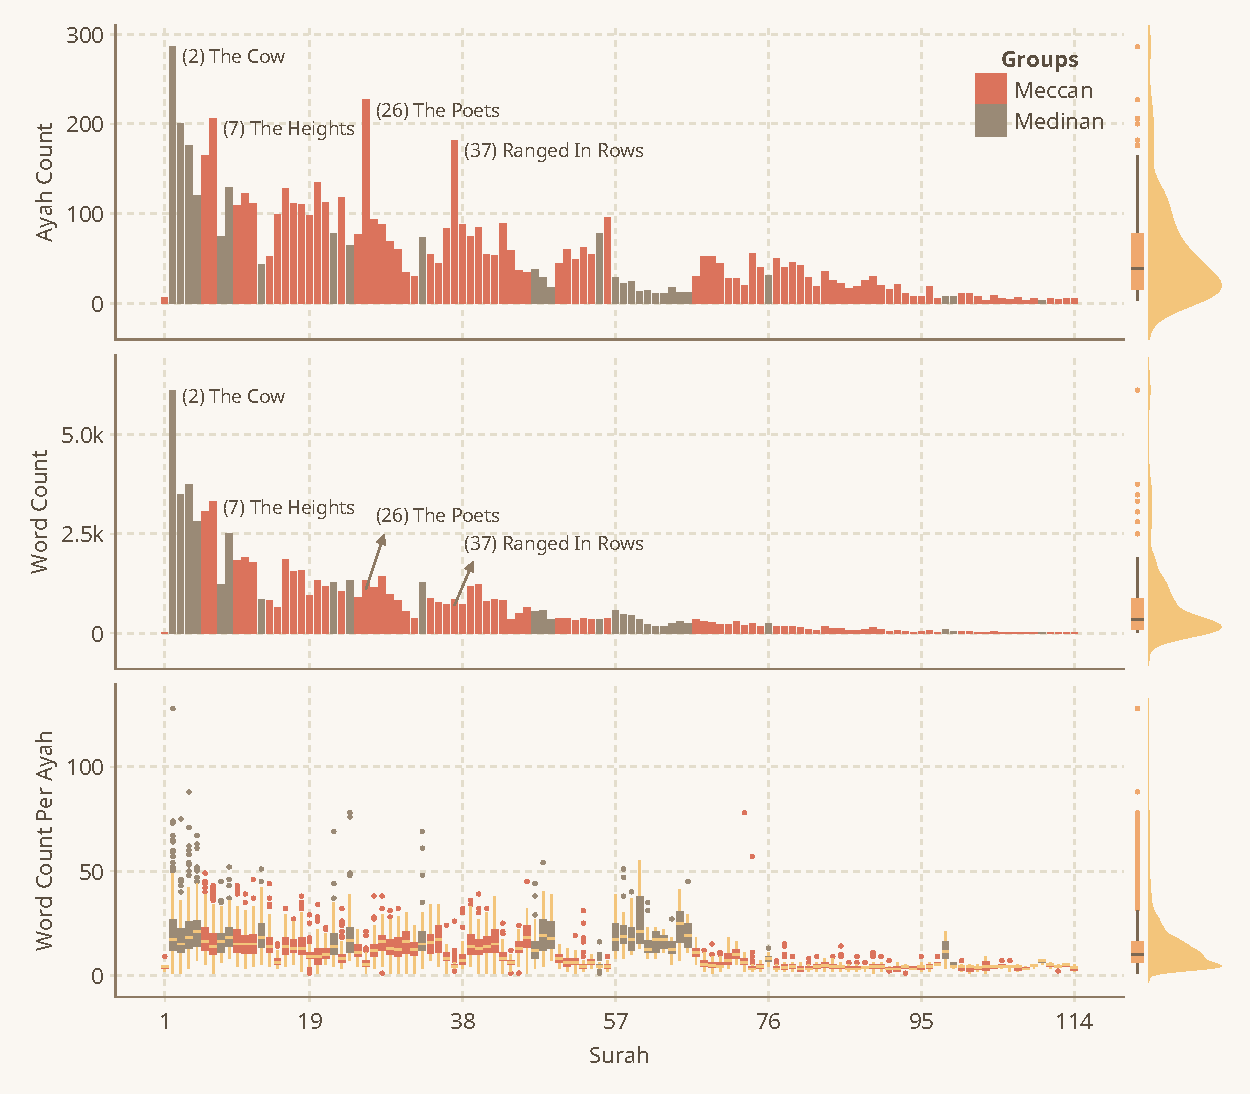
\includegraphics[width=\textwidth]{img/plot1.pdf}
    \caption{Statistics of the words and \arb[trans]{ayAt} \arb{ayAt} (verses) of the Qur'\=an}
    \label{fig:ayah_word_count_with_desc}
\end{figure}

As shown in Figure \ref{fig:ayah_word_count_with_desc}, both the Box and Density plots are tied to each other. This is indeed the case because both are describing the same information but presented in different style of visualization. In fact, Histogram is also used to describe the same information as the Box and Density, and the three are therefore related. So much so, that the three can be put into one graph. As to how to interpret these, readers are referred to for further details \textcolor{red}{[to add reference]}.
\begin{exmp}[Frequency Distribution]\label{ex:frequency_distribution}
Consider again the task of drawing an \arb[trans]{'ayAt} \arb{'ayAt} from the Qur'\=an, suppose the \arb[trans]{'ayAt} \arb{'ayAt} are separated into \arb{makkiyyaT} Meccan and \arb{madaniyyaT} Medinan, what is the probability of getting at most 10 \arb[trans]{kalimAt} \arb{kalimAt} or words in a sampled \arb[trans]{'ayAt} \arb{'ayAt} from \arb{makkiyyaT} Meccan \textit{surah}s \arb{sUr}?\\
\textit{Solution:} To answer this, Figure \ref{fig:meccan_medinan_word_count_per_ayah} shows the \textit{histograms} with the \textit{box plots} and the \textit{rainclouds} plots. The figure shows the frequency of the \arb[trans]{kalimAt} \arb{kalimAt} or words in a sampled \arb[trans]{'ayAt} \arb{'ayAt}. This frequency describes the distribution of the \arb[trans]{kalimAt} \arb{kalimAt}. To interpret this, the Medinan \arb{madaniyyaT} histogram shows that most of the \arb[trans]{'ayAt} \arb{'ayAt} have about 10 to 20 \arb[trans]{kalimAt} \arb{kalimAt} or words in total. This conclusion is based on the where the box of the box plot is located, which also corresponds to the area where the bars of the histogram are high, and also where most of the points or 'droplets' from the rainclouds plot are congested. With that said, \textit{historgram}, \textit{box plot}, and \textit{rainclouds} are related and are telling the same story from different perspectives. It should be noted that, the rainclouds plot is not a common visualization tool. 

Now, comparing the numbers from Medinan \arb{madaniyyaT} to the \arb[trans]{'AyAt 'l-makkiyyaTu} \arb{'AyAt 'l-makkiyyaTu}, there are about 5 to 15 \arb[trans]{kalimAt} \arb{kalimAt} to expect per \arb[trans]{'ayAt} \arb{'ayAt} based on Figure \ref{fig:meccan_medinan_word_count_per_ayah}. 

\begin{figure}[!t]
    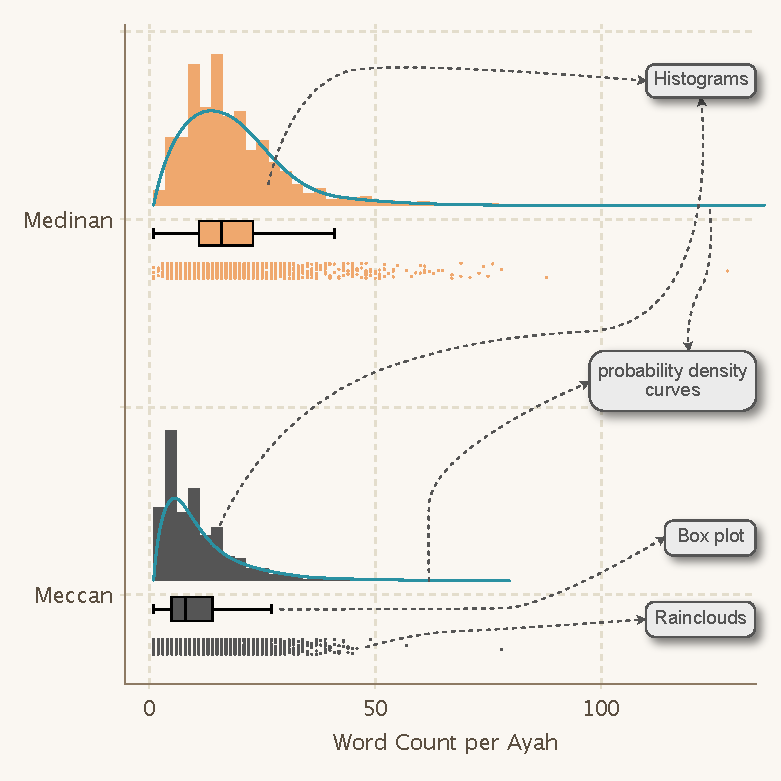
\includegraphics[width=\textwidth]{img/plot3.pdf}
    \caption{Probability density function plot of word count per \arb[trans]{'ayAt} \arb{'ayAt} by revelation location, in relation to its box plot and rainclouds.}
    \label{fig:meccan_medinan_word_count_per_ayah}
\end{figure}

The question has not been answered yet though, the above discussions only explains how to interpret the graphs in Figure \ref{fig:meccan_medinan_word_count_per_ayah}. So to answer the question, one simply needs to total the number of \arb[trans]{'AyAt} \arb{'AyAt} with at most 10 \arb[trans]{kalimAt} \arb{kalimAt} or words and divide this with the total number of \arb[trans]{'AyAt 'l-makkiyyaTu} \arb{'AyAt 'l-makkiyyaTu}. The answer is as follows, and this is part of the result of this paper: there are 4613 \arb[trans]{'AyAt 'l-makkiyyaTu} \arb{'AyAt 'l-makkiyyaTu}, and out of these is 2602 \arb[trans]{'AyAt 'l-makkiyyaTu} \arb{'AyAt 'l-makkiyyaTu} with at most 10 words. Therefore, the probability is $\frac{2602}{4613}=0.612$ or 61.2\% probability. Formally, if $X$ is the random variable of the event of observing at most 10 \arb[trans]{kalimAt} \arb{kalimAt} in a \arb[trans]{'AyAt 'l-makkiyyaTu} \arb{'AyAt 'l-makkiyyaTu}, then 
\begin{align}
     p(X\leq 10)=&\sum_{x=0}^{10} p(X=x)\label{ex_eq:prob_lesseq_10}\\
    =& p(X=0)+ p(X=1)+ p(X=2)+\cdots+ p(X=10)\label{ex_eq:freq_dist_prob1..10}\\
    =&0+\frac{24}{4613}+\frac{172}{4613}+\cdots+\frac{222}{4613}\label{ex_eq:freq_dist_probval1..10}\\
    =&\frac{2602}{4613}=0.612\label{ex_eq:prob_0612}
\end{align}

From Eq. \ref{ex_eq:freq_dist_prob1..10}, $ p(X=0)$ is the probability of observing zero \arb[trans]{kalimaT} \arb{kalimaT} in a \arb[trans]{'AyAt 'l-makkiyyaTu} \arb{'AyAt 'l-makkiyyaTu}, and $ p(X=1)$ is the probability of observing one \arb[trans]{kalimaT} \arb{kalimaT} in a \arb[trans]{'AyAt 'l-makkiyyaTu} \arb{'AyAt 'l-makkiyyaTu}, and so on. The numbers in Eq. \ref{ex_eq:freq_dist_probval1..10} are the number of \arb[trans]{'AyAt 'l-makkiyyaTu} \arb{'AyAt 'l-makkiyyaTu} having zero, one, two, to ten \arb[trans]{kalimAt} \arb{kalimAt}.

\end{exmp}
\section{Population and Sample}
Statistics is a branch of science that is concerned with understanding how the data behave based on a sample---a small set of the said data. It uses statistical methodologies to understand these behavior such as probability mass/density function, and use the findings from these tools on the sampled data as a conclusion for the population---the overall data.

Figure \ref{fig:pop_sample} illustrates the relation of population and sample data. A good example of this is the political surveys on the pulse of the nation on the candidates prior to election. Private entities like PulseAsia\footnote{\url{https://pulseasia.ph/}} and Social Weather Station\footnote{\url{https://www.sws.org.ph/swsmain/home/}} (SWS) do their survey by  sampling from the total population of the Philippines, hence the name survey.

The statistics computed from the surveys like the percentage of votes for particular political candidate are referred as estimates, this is because the computation was done in a sample of the population and not on the population itself. It is therefore important that for these estimates to be accurate representation of the nation's opinion, it has to be representative of the population. That is, the sample shouldn't be bias and leaning to the opinions of the few only and not of the whole nation.

The importance of the sample data as illustrated below follows from the fact that it saves time and cost since interviewing 2500 compared to 100,000 is better compromise for the estimated vote percentages. Further, since these samples requires to well represent the population, the computations of the statistics are estimated using statistical models, like probability mass/density functions, and other models like linear and nonlinears discussed in Section \ref{sec:stat_modeling}. The next example will illustrate the idea population and sample, and how probabilistic modeling can help in understanding insights and answering more questions.
\begin{figure}[t]
    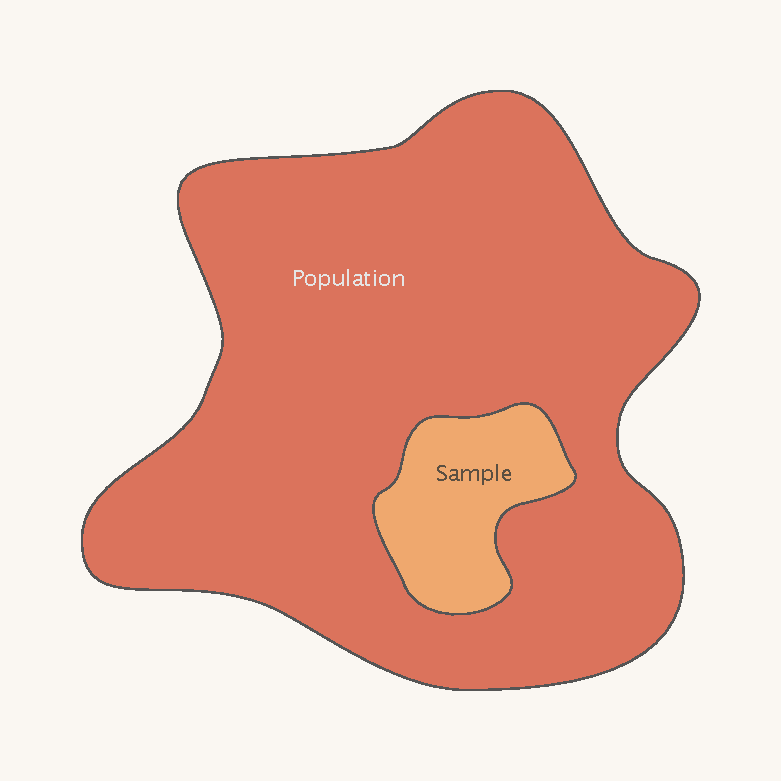
\includegraphics[width=\textwidth]{img/pop_sample.pdf}
    \caption{Population and sample illustration}
    \label{fig:pop_sample}
\end{figure}
\begin{exmp}\label{ex:population_sample_distribution_meccan_words}
Consider the task of sampling 250 \arb[trans]{'AyAt} \arb{'AyAt} from the population of \arb[trans]{'AyAt 'l-makkiyyaT}, describe the statistics of the population and the sample.\\
\textit{Solution:} In Statistics, there are several ways to sample from data, the simplest approach is through the use of \textit{uniform distribution}, that is, the sampling assumes that all data from the population are distributed equally, in the sense that all data points have equal chance of being selected. The other approach is through a \textit{weighted distribution}, where a probability is assigned to each of the data points in the population, so that, the selection will be biased to those with high probability. Figure \ref{fig:meccan_words_sampling} shows the graphs or plots of the population distribution of \arb[trans]{kalimAtu 'l-makkiyyaT} \arb{kalimAtu 'l-makkiyyaT}, which is presented as the top plot, this distribution of \arb{kalimAtu 'l-makkiyyaT} is the same one shown in the bottom plot of Figure \ref{fig:meccan_medinan_word_count_per_ayah}. 

To draw 100 samples from the said population, a simple random sampling without replacement (SRSWOR) is used for selecting or drawing samples. SRSWOR works by randomly selecting sample from the population and then setting it aside as the first sample. The resulting 100 samples are plotted in the bottom plot of Figure \ref{fig:meccan_words_sampling}.

As discussed above, the sample needs to be representative of the population. Figure \ref{fig:meccan_words_sampling} shows that the sampling distribution has more or less the same shape as the population. So that, the statistics are shown in Table \ref{tbl:meccan_words_pop_sample_stats}. From the said table, it can be seen that in terms of centrality, the both data are almost the same, for example the mean is 12.42 for the population and 10.64 for the sample. The reason why the mean in the population is much higher is due to the outlier in the population, which is seen in the extent of the tail of the Kernel Density Estimate in Figure \ref{fig:meccan_words_sampling}. In fact, this is seen in the Median in Table \ref{tbl:meccan_words_pop_sample_stats}, where  the estimate are almost the same. This is because the median is not affected by the outlier. However, the variance did suffer from the outlier in the population, with 50\% reduction in the sample variance, 54.15 to 48.96. The sample will less likely get the outlier as the sample since the outlier is only one observation from the 4163 total Meccan surahs.

The estimates got from the sample ideally are taken from a probabilistic model fitted into the sample data. This computation will be discussed in the next example.

\begin{table}
    \caption{Descriptive statistics of the population and sample data of \arb[trans]{kalimAtu 'l-makkiyyaT} \arb{kalimAtu 'l-makkiyyaT}}
    \label{tbl:meccan_words_pop_sample_stats}
    \begin{tabularx}{\textwidth}[!h]{XXXXl}
        \toprule
        Data&Mean&Median&Variance&Std. Deviation\\
        \midrule
        Population&10.28&8&54.15&7.36\\
        Sample&10.64&9&48.96&7.00\\
        \bottomrule
    \end{tabularx}
\end{table}
\begin{figure}[t]
    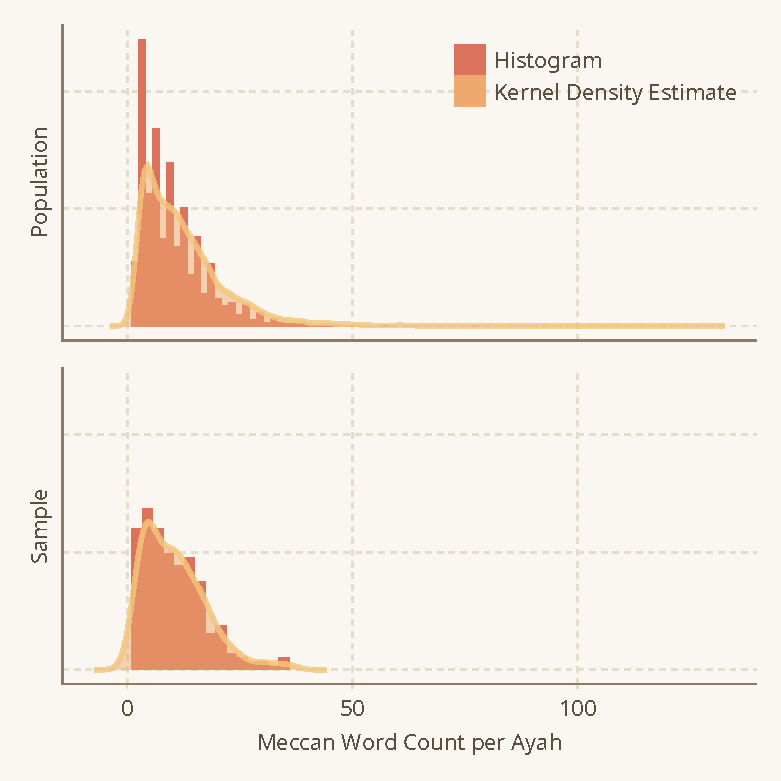
\includegraphics[width=\textwidth]{img/plot5.pdf}
    \caption{Population and sample distribution of Meccan }
    \label{fig:meccan_words_sampling}
\end{figure}

\end{exmp}
\begin{exmp}
Consider again Ex. \ref{ex:population_sample_distribution_meccan_words}, suppose the sample data is the only data available, how will you compute the probability of getting exactly 35 \arb[trans]{kalimAtu 'l-sUratu 'l-makkiyyaTu} \arb{kalimAtu 'l-sUratu 'l-makkiyyaTu}?\\
\textit{Solution:} To answer this question, one might approach this using the frequency distribution as in Ex. \ref{ex:frequency_distribution}. However, the use of frequency distribution from the said example is applicable since that deals with the population data, which is already the true probability, and there is no need to do some estimation. It is like try to get the average height of male Filipinos in the Philippines by doing census across the population, for such case, why would you do an estimate if you have all the census data of all heights of the Filipino, wouldn't it be easier to just do the average computation directly? This is the analogy for the frequency distribution used in Ex. \ref{ex:frequency_distribution}, that is, no need to do some estimation. However, for this problem, the assumption is that only the sample is available, that is, not all of the population is available. With that said, the best solution is to do some estimation. Now, doing an estimation is possible using the samples only, that is, using the idea of frequency distribution but this time applying it on the sample. This is becaus the sample was done using a random sampling, which more or less representative of the population. However, using this approach may possess a problem, let's see what that problem will likely be by forcing the approach in Ex. \ref{ex:frequency_distribution}, following the computation as in Eq. (\ref{ex_eq:prob_lesseq_10}) to Eq. (\ref{ex_eq:prob_0612}). 

Let $X$ again be the random variable of an event of observing 35 \arb[trans]{kalimAt} \arb{kalimAt}, this time from the sample, then
\begin{equation}\label{eq:probx_eq_35}
     p(X=35)=\begin{cases}
        \displaystyle\frac{0}{250}=0,&\text{if sample data}\\
        \displaystyle\frac{5}{4613}=0.0011,&\text{if population data}
    \end{cases}
\end{equation}
From the Eq. \ref{eq:probx_eq_35}, it shows that if we use the sample data for estimating the probability of observing 35 \arb{kalimAt}, then the answer above is 0, meaning by estimate there is a 0 chance of observing a 35 \arb{kalimAt} from a \arb[trans]{'AyAtu 'l-makkiyyaTu} \arb{'l-sUrAtu 'l-makkiyyaTu}. This conclusion is indeed misleading, since according to the population data, there are \arb[trans]{'AyAtu 'l-makkiyyaTu} \arb{'AyAtu 'l-makkiyyaTu} that has 35 \arb[trans]{kalimAt} \arb{kalimAt}. 

So, how to properly estimate this then? This is where the concept of probabilistic modeling comes in. For this problem, the data is count, and that the event of observing 10 \arb[trans]{kalimAtu 'l-sUratu 'l-makkiyyaTu} \arb{kalimAtu 'l-sUratu 'l-makkiyyaTu} in an \arb{'ayaT} is known to be best modeled by a Poisson distribution defined in Defn. \ref{defn:poisson_mass_function}. Ex. \ref{ex:poisson_distribution_sample} will discuss how to solve this. 
\end{exmp}
\section{Probability Distributions}
\begin{defn}[Poisson Mass Function]\label{defn:poisson_mass_function}
Let $X$ be a random variable and let $\lambda>0$ be a parameter, then if $x$ is the random value, then the \textit{Poisson} mass function is given by:
\begin{equation}
     p(X=x)=\frac{\lambda^x\exp(-\lambda)}{x!}
\end{equation}
\end{defn}
\begin{exmp}\label{ex:poisson_distribution_sample}
Consider again Ex. \ref{ex:population_sample_distribution_meccan_words}, the problem can be solved using the Poisson distribution.
\end{exmp}
\begin{defn}[Normal Density Function]
Let $Y$ be a random variable and let $\mu\in\mathbb{R}$ and $\sigma\in\mathbb{R}$ be the mean and variance parameters, if $y$ is the random value, then the \textit{Gaussian} or \textit{Normal} density function is given below:
\begin{equation}
     p(Y=y):=\frac{1}{\sqrt{2\pi\sigma^2}}\exp\left\{-\frac{(y-\mu)^2}{\sigma^2}\right\},\quad\text{where}\;-\infty<y<\infty
\end{equation}
\end{defn}
\begin{defn}[Dirichlet Density Function]
Let $\mathbf{Y}$ be a vector random variable with a random value $\mathbf{y}:=[y_1,\cdots,y_k]^{\text{T}}$ and let $\boldsymbol{\alpha}:=[\alpha_1,\cdots,\alpha_k]^{\text{T}}$ be the parameters, then the \textit{Dirichlet} density function is defined as
\begin{equation}
     p(\mathbf{X}=\mathbf{x};\boldsymbol{\alpha}):=\frac{1}{B(\boldsymbol{\alpha})}\prod_{i=1}^kx_i^{\alpha_i-1},
\end{equation}
where,
\begin{equation}
    B(\boldsymbol{\alpha}):=\frac{\displaystyle\prod_{i=1}^k\Gamma(\alpha_i)}{\Gamma\left(\sum_{i=1}^k\alpha_i\right)}
\end{equation}

\end{defn}
\begin{defn}[Multinomial Mass Function]
Let $\mathbf{X}$ be a vector random variable with a random value $\mathbf{x}:=[x_1,\cdots,x_k]^{\text{T}}$ such that $x_i\geq 0,\forall i \in[1,k]$, let $\boldsymbol{q}:=[q_1,\cdots,q_k]^{\text{T}}$ and $n$ be the parameters, the probability mass function of a Multinomial distribution is 
\begin{align}
    f(x_1,\cdots,x_k;n,q_1,\cdots,q_k):=& q(X_1=x_1\;\text{and}\;\cdots\;\text{and}\;X_k=x_k)\nonumber\\
    =&\begin{cases}
        \displaystyle\frac{n!}{x_1!\cdots x_k!}q_1^{x_1}\times\cdots\times q_k^{x_k},&\text{when}\;\sum_{i=1}^kx_i=n\\
        0&\text{otherwise},
    \end{cases}
\end{align}
\end{defn}

\section{Frequentist Estimation}\label{sec:stat_modeling}
Probability distributions are fundamental models that can be used to describe some characteristics of the data. However, combinations of variables, and accounting dynamics of the observations can lead into other types of models as well. In general, a statistical model can be written using the following formula:
\begin{equation}
    y=f(x|\mathbf{\Theta})+\varepsilon,
\end{equation}
where $y\sim p(\cdot)$ and $\varepsilon\sim p(\cdot)$.

There are two main ways to estimating the parameters $\boldsymbol{\Theta}$, and that is either through Frequentist or Bayesian approach.
\subsection{Maximum Likelihood Estimation}
Maximum likelihood estimation (MLE) is a fundamental concept in statistics that provides a method for estimating the parameters of a statistical model based on the observed data. The basic idea behind MLE is to find the parameter values that make the observed data most likely or probable under the assumed statistical model. The concept of MLE can be explained as follows:

Suppose we have a random sample of observations $X := \{x_1, x_2, ..., x_n\}$ from a probability distribution $f(x | \theta)$, where $\theta$ represents the unknown parameter(s) of the distribution. The likelihood function, denoted as $\mathcal{L}(\theta | X)$, is the joint probability density (or probability mass function for discrete distributions) of the observed data $X$, treated as a function of the parameter(s) $\theta$.
\begin{equation}
    \mathcal{L}(\theta | X) = f(x_1 | \theta) \times f(x_2 | \theta) \times\cdots\times f(x_n | \theta)    
\end{equation}

The maximum likelihood estimate (MLE) of $\theta$, denoted as $\hat{\theta}$, is the value of $\theta$ that maximizes the likelihood function $\mathcal{L}(\theta | X)$. In other words, $\hat{\theta}$ is the value of θ that makes the observed data most likely or probable under the assumed statistical model.
\begin{equation}
    \hat{\theta} = \underset{\theta}{\arg\max} \mathcal{L}(\theta | X)    
\end{equation}

In practice, it is often easier to work with the log-likelihood function, denoted as $\ell(\theta | X) = \log(\mathcal{L}(\theta | X))$, since the logarithm is a monotonic function and maximizing the log-likelihood is equivalent to maximizing the likelihood.
\begin{equation}
   \hat{\theta} = \underset{\theta}{\arg\max}\ell(\theta | X)    
\end{equation}
\begin{exmp}[Normal distribution]
    Suppose we have a random sample $X = \{x_1, x_2,\cdots, x_n\}$ from a normal distribution with unknown mean μ and known variance $\sigma^2$. The likelihood function is:
    \begin{equation}
        \mathcal{L}(\mu | X) = \frac{1}{(\sqrt{2\pi\sigma^2})^n}\exp\left(-\sum_{\forall i}(x_i - \mu)^2 / (2\sigma^2)\right)
    \end{equation}
    
    Taking the log and differentiating with respect to $\mu$, setting the derivative equal to zero, and solving for $\mu$, we get the maximum likelihood estimate or MLE of $\mu$:
    \begin{equation}
        \hat{\mu} = \frac{1}{n}\sum_{\forall i}x_i
    \end{equation}
\end{exmp}
MLE has several desirable properties, such as consistency (the MLE converges to the true parameter value as the sample size increases) and asymptotic normality (the sampling distribution of the MLE approaches a normal distribution as the sample size increases), which make it a widely used method in statistical inference and modeling.
\subsection{Numerical Approximation}
There are several ways to numerically estimate the parameters of the model using mathematical programming. The popular algorithm that is very common in Machine Learning is the \textit{gradient descent} (GD) given in Algorithm \ref{algo:GD}. Suppose $\nabla\ein(\hat{\mathbf{w}}^{(r)})$ is the gradient of the cost function at the $r$th iteration. $\ein$ is defined as \mbox{the \textit{in-sample error}} or the error in the training dataset, $\gamma$ is the \textit{learning-rate} parameter of the algorithm and $\nu$ is the \textit{precision} parameter. As an illustration, consider Example \ref{ex:gd}.\vspace{.4cm}

\begin{algorithm}
\caption{\it Gradient Descent}
\label{algo:GD}
\begin{algorithmic}[1]\vspace{.2cm}
\item Initialize $\hat{\mathbf{w}}^{(r)},r=0$\vspace{.2cm}
\While{$\lVert \hat{\mathbf{w}}^{(r+1)}-\hat{\mathbf{w}}^{(r)}\rVert > \nu$}\vspace{.2cm}
\State $\hat{\mathbf{w}}^{(r+1)}\triangleq \hat{\mathbf{w}}^{(r)} - \gamma\nabla\ein(\hat{\mathbf{w}}^{(r)})$\vspace{.2cm}
\State $r\triangleq r + 1$\vspace{.2cm}
\EndWhile\\\vspace{.2cm}
\Return $\hat{\mathbf{w}}^{(r)}$ and $r$.
\end{algorithmic}
\end{algorithm}
\vspace{-.3cm}

\begin{exmp}\label{ex:gd}
Suppose the loss function is given by
\begin{equation}\label{eq:errgd1}
\ein(w)\triangleq w^4 - 3w^3 + 2.
\end{equation}
The first derivative of the above equation with respect to $w$ is given by ${\ein'(w)=4w^3-9w^2}$. Let the initial guess be $\hat{w}^{(0)}=.1$ and let $\gamma=.01$ with $\nu=.00001$. Then $\nabla\ein(\hat{w}^{(0)})=\ein'(\hat{w}^{(0)})=-0.086$, so that $\hat{w}^{(1)}\triangleq\hat{w}^{(0)}-.01(-0.086)=0.10086$, and $|\hat{w}^{(1)} - \hat{w}^{(0)}| = 0.00086> \nu$. It turns out that 173 iterations are needed to satisfy \mbox{the inequality}, $|\hat{w}^{(r+1)} - \hat{w}^{(r)}| \ngtr \nu$.
\end{exmp}
In practice, however, there are hundreds to millions of data points that need to be summarized, so that at each iteration, the parameters are updated \textit{after} \mbox{the presentation} of \textit{all} the training examples that constitute an \textit{epoch} --- one complete presentation of the entire training dataset during the learning process \cite{Haykin1998}. In this setting, GD is sometimes called \textit{batch gradient descent} (BGD).
\subsection{Stochastic Gradient Descent}\label{sec:sgd}
An alternative to BGD is SGD or \textit{stochastic gradient descent}. SGD updates the parameter using only one observation for every iteration, which is a lot faster. Further, BGD is prone to local minimum since GD does so. This is guaranteed for misspecified initial value especially for high dimensional nonlinear error surface function. \mbox{The stochasticity} of the SGD follows from the randomization of the dataset at each epoch, and contrary to BGD, the SGD is not expected to converge to \mbox{the global} minimum, instead it will only stay around the global solution (\textit{see} Algorithm \ref{algo:SGD}). Example \ref{exmp:bgdslr} illustrates the application of mathematical programming in estimating the parameters of a simple linear regression model.
\vspace{.4cm}

\begin{algorithm}[!h]
\caption{\it Stochastic Gradient Descent}
\label{algo:SGD}
\begin{algorithmic}[1]\vspace{.2cm}
\item Initialize $\hat{\mathbf{w}}^{(r)},r=0$\vspace{.2cm}
\While{$\lVert \hat{\mathbf{w}}^{(r)}-\hat{\mathbf{w}}^{(r+1)}\rVert > \nu$}\vspace{.2cm}
\State Randomize the data set ($\mathbf{x}_i,\mathbf{y}_i$) with respect to $i$.\vspace{.2cm}
\For{$i \in\{1,\cdots, n\}$}\vspace{.2cm}
\State Update the parameters
\begin{align}\nonumber
\hat{\mathbf{w}}^{(r)}&\triangleq \hat{\mathbf{w}}^{(r)} - \gamma\nabla\mathrm{e}(h(\mathbf{x}_i,\hat{\mathbf{w}}^{(r)}),\mathbf{y}_i)\\\nonumber
&=\hat{\mathbf{w}}^{(r)} - \gamma\frac{\partial}{\partial\mathbf{w}}\left\{\frac{1}{2}[h(\mathbf{x}_i,\hat{\mathbf{w}}^{(r)})-\mathbf{y}_i]^2\right\}
\end{align}
%\State Compute $\mathrm{e}^{(r)}\triangleq\mathrm{e}(h(\mathbf{x}_k,\hat{\mathbf{w}}^{(r+1)}),\mathbf{y}_k)$\vspace{.2cm}
\EndFor\vspace{.2cm}
\State $\hat{\mathbf{w}}^{(r+1)}\triangleq \hat{\mathbf{w}}^{(r)}$\vspace{.2cm}
%\State Compute the cost function
%\begin{equation}
%\ein(h)=\frac{1}{n}\sum_{i=1}^K\mathrm{e}(h(\mathbf{x}_i,\hat{\mathbf{w}}^{(r+1)}),\mathbf{y}_i)
%\end{equation}
\EndWhile\vspace{.2cm}
\item\Return $\hat{\mathbf{w}}^{r}$ and $r$.
\end{algorithmic}
\end{algorithm}
\section{Bayesian Estimation}
Bayesian estimation is a statistical approach that incorporates prior knowledge or beliefs about the parameters of interest into the estimation process. It combines the prior knowledge with the observed data to obtain updated beliefs or estimates of the parameters, known as the posterior distribution.
The Bayesian estimation framework is based on Bayes' theorem, which relates the conditional probabilities of events. In the context of parameter estimation, Bayes' theorem can be expressed as:
\begin{equation}
    p(\theta | X) = \frac{p(X | \theta)p(\theta))}{p(X)}
\end{equation}
where $p(\theta | X)$ is the posterior distribution, representing the updated beliefs about the parameter(s) $\theta$ after observing the data X. $p(X | \theta)$ is the likelihood function, which quantifies the probability of observing the data X given the parameter(s) $\theta$. $p(\theta)$ is the prior distribution, representing the initial beliefs or knowledge about the parameter(s) $\theta$ before observing the data. $p(X)$ is the marginal likelihood or the probability of observing the data X, which acts as a normalizing constant.
\subsection{Laplace's Approximation}\label{sec:laplace}
The simplest approximation to the posterior distribution of the parameter of interest is the Laplace's approximation. The idea behind this procedure is to use a Gaussian approximator, $\g(x)$, such that it is centered on the mode of the target distribution, $ p(x)$. To illustrate, suppose
\begin{equation}
 p(x):=\frac{f(x)}{Z},\quad\mathrm{where}\;Z:=\int f(x)\D x.
\end{equation}
Using basic calculus, the mode\footnote{obtained using maximum \textit{a posteriori} (MAP)} of the posterior distribution, say at $x=x_{\text{MAP}}$, is achieved by taking the derivative of the objective function with respect to the $x$-axis, such that the gradient of the function is $0$ at $x=x_{\text{MAP}}$. That is,
\begin{equation}
\frac{\D f(x)}{\D x}\bigg|_{x=x_{\text{MAP}}}=0.
\end{equation}
The Gaussian distribution has the property that its logarithm is a quadratic function of the variables \cite{bishop}. Hence, the following is an approximation of \mbox{the log} of \mbox{the objective} function using second-order Taylor series expansion centered on \mbox{the mode} $x_{\text{MAP}}$, 
\begin{align}
\log f(x)=&\log f(x_{\text{MAP}})+\frac{\D \log f(x)}{\D x}\bigg|_{x=x_{\text{MAP}}}(x-x_{\text{MAP}})\\
&+\frac{\D^2 \log f(x)}{\D x^2}\bigg|_{x=x_{\text{MAP}}}\frac{(x-x_{\text{MAP}})^2}{2}+\mathcal{O}(x)\\
\approx&\log f(x_{\text{MAP}})+\frac{\D^2 \log f(x)}{\D x^2}\bigg|_{x=x_{\text{MAP}}}\frac{(x-x_{\text{MAP}})^2}{2}.
\end{align}
Exponentiating both sides of the above equations becomes
\begin{equation}
f(x)\approx f(x_{\text{MAP}})\exp\left[\frac{\D^2 \log f(x)}{\D x^2}\bigg|_{x=x_{\text{MAP}}}\frac{(x-x_{\text{MAP}})^2}{2}\right],
\end{equation}
so that the normalized estimator $\g(x)$ is given by
\begin{equation}
\g(x)=\left(-\frac{1}{2\pi}\frac{\D^2 \log f(x)}{\D x^2}\bigg|_{x=x_{\text{MAP}}}\right)^{1/2}\exp\left[\frac{\D^2 \log f(x)}{\D x^2}\bigg|_{x=x_{\text{MAP}}}\frac{(x-x_{\text{MAP}})^2}{2}\right].
\end{equation}
\vspace{-1cm}
\begin{exmp}
Suppose the posterior distribution is a chi-square of the form: $p(x):=\frac{x^{k-1}\exp\left(-\frac{x^2}{2}\right)}{Z}$, with $k$ degrees of freedom where $Z:=2^{\frac{k}{2}-1}\Gamma\left(\frac{k}{2}\right),\quad x>0$. Using Laplace, \mbox{the approximator} to the posterior distribution is obtained as follows:\\[.3cm]
The log-likelihood of the density function is given by
\begin{equation}
\ell(x):=\log p(x)=(k-1)\log x-\frac{x^2}{2}+\mathcal{C},
\end{equation}
where $\mathcal{C}$ is the constant. The mode of this posterior is given by
\begin{align}
\frac{\partial}{\partial x}\log  p(x)&=\frac{k-1}{x_{\text{MAP}}}-x_{\text{MAP}}\overset{\text{set}}{=}0\\
x_{\text{MAP}}&=\sqrt{k-1}.
\end{align}
The second partial derivative of the log-likelihood with respect to $x$ evaluated at $x_{\text{MAP}}$ is
\begin{equation}\label{eq:laplaceexapprox}
-\frac{\partial^2}{\partial x^2}\log  p(x)\bigg|_{x=x_{\text{MAP}}}=1-\frac{1-k}{x_{\text{MAP}}^2}=2.
\end{equation}
Thus the estimate of the posterior is given by a Gaussian distribution with mean $\mu=\sqrt{k-1}$ and variance $\sigma^2 = \frac{1}{2}$. Figure \ref{fig:laplaceapprox} visualizes the Gaussian distribution as an approximator to the posterior distribution.
\end{exmp}
Now consider the case where $\mathbf{x}\in\mathbb{R}^{d}$, such that $ p(\mathbf{x}):=\frac{f(\mathbf{x})}{Z}$. Analogous to \mbox{the univariate} case, the Laplace's approximation for $ p(\mathbf{x})$ is obtained by aligning \mbox{the mean} of the multivariate Gaussian distribution to the mode of the posterior density, denoted by $\mathbf{x}_{\text{MAP}}$. As before, the log-likelihood of $f(\mathbf{z})$ is given by \mbox{the following} equation
\begin{equation}\label{eq:laplacemultivar}
\log f(\mathbf{x})\approx\log f(\mathbf{x}_{\text{MAP}})-\frac{1}{2}(\mathbf{x}-\mathbf{x}_{\text{MAP}})^{\text{T}}\boldsymbol{\mathfrak{H}}(\mathbf{x}-\mathbf{x}_{\text{MAP}}),
\end{equation}
where $\boldsymbol{\mathfrak{H}}$ is the Hessian matrix defined by
\begin{equation}\label{eq:2ndderivlaplace}
\boldsymbol{\mathfrak{H}}:=-\frac{\partial^2}{\partial\mathbf{x}^2}\log f(\mathbf{x})\bigg|_{\mathbf{x}=\mathbf{x}_{\text{MAP}}}.
\end{equation}
Exponentiating Equation (\ref{eq:laplacemultivar}) leads to the normalized approximator, $\g(\mathbf{x})=\mathcal{N}_d(\mathbf{x}|\mathbf{x}_{\text{MAP}},\boldsymbol{\mathfrak{H}}^{-1})$.
\subsection{Markov Chain Monte Carlo (MCMC)}
Laplace has the advantage of being simple and easy to use. However, like any approximator, it has limitations especially on multimodal densities since it uses Gaussian as estimate to the posterior distribution. Most interesting high dimensional Bayesian models have multimodal \textit{a posteriori}, which can't be captured through Laplace's method. To address this problem, sampling methods are instead used for approximating the \textit{a posteriori}. These family of sampling methods are called Markov Chain Monte Carlos (MCMC) with \textit{Metropolis-Hasting} (MH) and \textit{Gibbs sampling} as \mbox{the popular} MCMCs. Further, for sophisticated MCMCs, the algorithms available are not limited to \textit{Hamiltonian Monte Carlo} (HMC) and \textit{Stochastic Gradient HMC}.
\subsection{Metropolis-Hasting}\label{sec:metropolishasting}
The idea of the MH algorithm is to randomly walk in the support of the target density such that the random step is governed by the proposal distribution $\g(\cdot)$. \mbox{The assumption} is that the posterior distribution has no closed-form solution, but the kernel, which is the unnormalized form of the target density is easy to evaluate. This is the advantage of the Metropolis-Hasting algorithm where the \textit{a posteriori} is not necessarily be normalized --- often the difficulty in simplifying the model evidence of the Bayes' rule. Let $ p(\cdot)$ be the \textit{a posteriori}, then the Metropolis-Hasting algorithm is given in Algorithm \ref{algo:mcmcmh}.
\vspace{.4cm}

\begin{algorithm}[!t]
\caption{\it Metropolis-Hasting MCMC}
\label{algo:mcmcmh}
\begin{algorithmic}[1]\vspace{.2cm}
\item Initialize $\mathbf{w}_{r}\sim\g(\mathbf{w}),r=0$\vspace{.2cm}
\For {$r\in\{1,\cdots, r_{\text{max}}\}$}\vspace{.2cm}
\State Propose: $\mathbf{w}_{new}\sim\g(\mathbf{w}_{new}|\mathbf{w}_{r-1})$\vspace{.2cm}
\State Acceptance: $\alpha(\mathbf{w}_{new}|\mathbf{w}_{r-1}):=\min\left\{1,\frac{ p(\mathbf{w}_{new}|\mathbf{w}_{r-1})\g(\mathbf{w}_{r-1}|\mathbf{w}_{new})}{ p(\mathbf{w}_{r-1}|\mathbf{w}_{new})\g(\mathbf{w}_{new}|\mathbf{w}_{r-1})}\right\}$\vspace{.2cm}
\State Draw $x\sim\text{Unif}(0,1)$\vspace{.2cm}
\If {$x<\alpha(\mathbf{w}_{new}|\mathbf{w}_{r-1})$}\vspace{.2cm}
\State $\mathbf{w}_{r}:=\mathbf{w}_{new}$
\vspace{.2cm}
\Else \vspace{.2cm}
\State $\mathbf{w}_{r}:=\mathbf{w}_{r-1}$\vspace{.2cm}
\EndIf\vspace{.2cm}
\EndFor
\end{algorithmic}
\end{algorithm}
\vspace{-.3cm}
\begin{exmp}\label{exmp:mcmcmh}
Consider the bivariate Gaussian distribution defined below:
\begin{equation}
f(\mathbf{x}|\boldsymbol{\mu},\boldsymbol{\Sigma})
:=\frac{1}{\sqrt{(2\pi)^d|\boldsymbol{\Sigma}|}}\exp\left[-\frac{1}{2}(\mathbf{x} - \boldsymbol{\mu})^{\text{T}}\boldsymbol{\Sigma}^{-1}(\mathbf{x}-\boldsymbol{\mu})\right].
\end{equation}
Suppose it has the following parameters: 
\begin{equation}\nonumber
\boldsymbol{\mu}:=[10\;-10]^{\text{T}} \quad\text{and}\quad \boldsymbol{\Sigma}:=\left[\begin{array}{cc}1.5^2&\rho(1.5)(1.35)\\\rho(1.5)(1.35)&1.35^2\end{array}\right]
\end{equation}
where ${\rho := .5}$; in order to draw samples from this model, let the proposal distribution defined to be the current step of the random walk plus an increment from a uniform distribution with parameters min = -5 and max = 5.

The random samples drawn by MH are not independent, this is due to \mbox{the design} of the algorithm where the distribution of the candidate sample depends solely on the current sample\footnote{this is the property of the Markov Chain, hence the name MCMC.}. To address this problem, diagnostics are applied using methods such as \textit{thinning}, where every $i$th sample is taken and the rest are discarded; or using \textit{burn-in} where first $n^{\star}$ samples are discarded.

\end{exmp}
\subsection{Gibbs Sampling}\label{sec:gibbssampling}
MH is by far one of the easiest MCMC algorithm for drawing samples from \textit{a posteriori} where direct sampling is not possible. It uses proposal distribution as drivers of the random walk in the support of the target density, which for high dimensional data, the choice of appropriate proposal function is sometimes difficult to specify. As an alternative, Gibbs sampler can be used for taking samples from the posterior distribution. The only requirement is that the joint distribution of the parameters (the \textit{a posteriori}) can be decomposed into conditional distributions of each variable conditioned on other variables. Mathematically, suppose \mbox{the multivariate} distribution is given by $f(\mathbf{w}|\mathscr{D})$, where $\mathbf{w}:=[w_1\;w_2\cdots w_K]^{\text{T}}$, then the Gibbs sampling algorithm is given in Algorithm \ref{algo:mcmcgibbs}.
\vspace{.4cm}

\begin{algorithm}[!b]
\caption{\it Gibbs Sampling MCMC}
\label{algo:mcmcgibbs}
\begin{algorithmic}[1]\vspace{.2cm}
\item Initialize $\mathbf{w}_{r}, r=0$\vspace{.2cm}
\For {$r\in\{1,\cdots, r_{\text{max}}\}$}\vspace{.2cm}
\State $w_1^{(new)}\sim f(w_1|w_2,\cdots,w_K)$\vspace{.2cm}
\State $w_2^{(new)}\sim f(w_2|w_1^{(new)},\cdots,w_K)$\vspace{.2cm}
\State $w_3^{(new)}\sim f(w_3|w_1^{(new)},w_2^{(new)},\cdots,w_K)$\vspace{.2cm}
\State $\vdots\qquad\qquad\qquad\vdots\qquad\qquad\qquad\vdots$\vspace{.2cm}
\State $w_K^{(new)}\sim f(w_K|w_1^{(new)},w_2^{(new)},\cdots,w_{K-1}^{(new)})$\vspace{.2cm}
\State $\mathbf{w}_r:=[w_1^{(new)},\cdots,w_K^{(new)}]^{\text{T}}$\vspace{.2cm}
\EndFor
\end{algorithmic}
\end{algorithm}
\vspace{-.3cm}
\begin{exmp}\label{exmp:gibbs}
Using the same posterior distribution as in Example \ref{exmp:mcmcmh}, the conditional distributions of the parameters conditioned on other parameters are also Gaussian with mean $\mu:=\mu_1 + \left(\frac{\sigma_1}{\sigma_2}\right)\rho(x - \mu_2)$ and standard deviation $\sigma:=\sqrt{(1 - \rho^2)\sigma_1^2}$. Analogous to MH, samples obtained using Gibbs are not independent but with lower autocorrelation compared to the former. As before, the same diagnostics can be done. 
\end{exmp}
\subsection{Bayesian Linear Regression}\label{sec:blr}
As an illustration of Bayesian inference to basic modeling, this section attempts to discuss the Bayesian approach to linear regression. Let ${\mathscr{D}=\{(\mathbf{x}_1,y_1),\cdots, (\mathbf{x}_n,y_n)\}}$ where $\mathbf{x}_i\in\mathbb{R}^{d}, y_i\in \mathbb{R}$ be the pairwised dataset. Suppose the response values, $y_1,\cdots,y_n$, are independent given the parameter $\mathbf{w}$, and is distributed as $y_i\sim\mathcal{N}(\mathbf{w}^{\text{T}}\mathbf{x}_i,\alpha^{-1})$, where $\alpha^{-1}$ is referred to as the \textit{precision} parameter --- useful for later derivation. In Bayesian perspective, the weights are assumed to be random and are governed by some \textit{a priori} distribution. The choice of this distribution is subjective, but choosing arbitrary \textit{a priori} can sometimes or often result to an intractable integration, especially for interesting models. For simplicity, a conjugate prior is used for the latent weights. Specifically, assume that ${\mathbf{w}\sim\mathcal{N}(\mathbf{0},\beta^{-1}\mathbf{I})}$ such that $\beta>0$ is the hyperparameter supposed in this experiment as known value. The posterior distribution based on the Bayes' rule is given by
\begin{equation}\label{eq:bayesrulepost}
	p(\mathbf{w}|\mathbf{y})=\frac{p(\mathbf{w})p(\mathbf{y}|\mathbf{w})}{p(\mathbf{y})},
\end{equation}
where $p(\mathbf{w})$ is the \textit{a priori} distribution of the parameter, $p(\mathbf{y}|\mathbf{w})$ is the likelihood, and $p(\mathbf{y})$ is the normalizing factor. The likelihood is given by
\begin{align}
    p(\mathbf{y}|\mathbf{w})&=\prod_{i=1}^{n}\frac{1}{\sqrt{2\pi\alpha^{-1}}}\exp\left[-\frac{\alpha(y_i-\mathbf{w}^{\text{T}}\mathbf{x}_i)^2}{2}\right]\\
    &=\left(\frac{\alpha}{2\pi}\right)^{n/2}\exp\left[-\sum_{i=1}^n\frac{\alpha(y_i-\mathbf{w}^{\text{T}}\mathbf{x}_i)^2}{2}\right].\label{eq:likelihood:blreg}
\end{align}
In matrix form, this can be written as
\begin{equation}
    p(\mathbf{y}|\mathbf{w})\propto\exp\left[-\frac{\alpha}{2}(\mathbf{y}-\boldsymbol{\mathfrak{A}}\mathbf{w})^{\text{T}}(\mathbf{y}-\boldsymbol{\mathfrak{A}}\mathbf{w})\right]
\end{equation}
where $\boldsymbol{\mathfrak{A}}=\left[(\mathbf{x}_i^{\text{T}})\right]$, i.e. $\boldsymbol{\mathfrak{A}}\in(\mathbb{R}^{n}\times\mathbb{R}^d)$, this matrix is known as the \textit{design matrix}. Given that $\mathbf{w}$ has the following prior distribution
\begin{equation}\label{eq:wpriori}
    p(\mathbf{w})=\frac{1}{\sqrt{(2\pi)^{d}|\beta^{-1}\mathbf{I}|}}\exp\left[-\frac{1}{2}\mathbf{w}^{\text{T}}\beta\mathbf{I}\mathbf{w}\right],
\end{equation}
implies that the posterior has the following form:
\begin{align}
    p(\mathbf{w}|\mathbf{y})&\propto\exp\left[-\frac{\alpha}{2}(\mathbf{y}-\boldsymbol{\mathfrak{A}}\mathbf{w})^{\text{T}}(\mathbf{y}-\boldsymbol{\mathfrak{A}}\mathbf{w})\right]\exp\left[-\frac{1}{2}\mathbf{w}^{\text{T}}\beta\mathbf{I}\mathbf{w}\right]\\
&=\exp\left\{-\frac{1}{2}\left[\alpha(\mathbf{y}-\boldsymbol{\mathfrak{A}}\mathbf{w})^{\text{T}}(\mathbf{y}-\boldsymbol{\mathfrak{A}}\mathbf{w})+\mathbf{w}^{\text{T}}\beta\mathbf{I}\mathbf{w}\right]\right\}.
\end{align}
Expanding the terms in the exponent, becomes
\begin{equation}\label{eq:expterms}
    \alpha\mathbf{y}^{\text{T}}\mathbf{y}-2\alpha\mathbf{w}^{\text{T}}\boldsymbol{\mathfrak{A}}^{\text{T}}\mathbf{y}+\mathbf{w}^{\text{T}}(\alpha\boldsymbol{\mathfrak{A}}^{\text{T}}\boldsymbol{\mathfrak{A}}+\beta\mathbf{I})\mathbf{w}.
\end{equation}
The next step is to complete the square of the above equation such that it resembles the inner terms of the exponential factor of the Gaussian distribution. The quadratic form of the exponential term of a $\mathcal{N}(\mathbf{w}|\boldsymbol{\mu},\boldsymbol{\Sigma}^{-1})$ is given by
\begin{align}
    (\mathbf{w}-\boldsymbol{\mu})^{\text{T}}\boldsymbol{\Sigma}^{-1}(\mathbf{w}-\boldsymbol{\mu})&=(\mathbf{w}-\boldsymbol{\mu})^{\text{T}}(\boldsymbol{\Sigma}^{-1}\mathbf{w}-\boldsymbol{\Sigma}^{-1}\boldsymbol{\mu})\\
&=\mathbf{w}^{\text{T}}\boldsymbol{\Sigma}^{-1}\mathbf{w}-
2\mathbf{w}^{\text{T}}\boldsymbol{\Sigma}^{-1}\boldsymbol{\mu}+\boldsymbol{\mu}^{\text{T}}\boldsymbol{\Sigma}^{-1}\boldsymbol{\mu}.\label{eq:expnorm}
\end{align}
The terms in Equation (\ref{eq:expterms}) are matched up with that in (\ref{eq:expnorm}), so that
\begin{equation}\label{eq:sigmablrgauss}
    \boldsymbol{\Sigma}^{-1}=\alpha\boldsymbol{\mathfrak{A}}^{\text{T}}\boldsymbol{\mathfrak{A}}+\beta\mathbf{I}
\end{equation}
and
\begin{align}
    \mathbf{w}^{\text{T}}\boldsymbol{\Sigma}^{-1}\boldsymbol{\mu}&=\alpha\mathbf{w}^{\text{T}}\boldsymbol{\mathfrak{A}}^{\text{T}}\mathbf{y}\\
    \boldsymbol{\Sigma}^{-1}\boldsymbol{\mu}&=\alpha\boldsymbol{\mathfrak{A}}^{\text{T}}\mathbf{y}\\
    \boldsymbol{\mu}&=\alpha\boldsymbol{\Sigma}\boldsymbol{\mathfrak{A}}^{\text{T}}\mathbf{y}.\label{eq:mublrgauss}
\end{align}
Thus the \textit{a posteriori} is a Gaussian distribution with location parameter in \mbox{Equation (\ref{eq:mublrgauss})} and scale parameter given by the inverse of Equation (\ref{eq:sigmablrgauss}).
\section{Types of Statistical Methods}
\textit{Parametric} and \textit{non-parametric} statistics are two broad categories of statistical methods, each with its own assumptions and applications. The primary difference between them lies in the underlying assumptions made about the population distribution.
\subsection{Parametric}
Parametric statistics are based on the assumption that the data follows a specific probability distribution, such as the normal distribution (also known as the Gaussian distribution). These methods rely on the estimation of parameters (such as the mean and standard deviation) from the sample data to make inferences about the population.
\begin{enumerate}
    \item \textbf{Student's t-test} - for comparing means
    \item \textbf{Analysis of Variance (ANOVA)} - for comparing means across multiple groups
    \item \textbf{Pearson's correlation coefficient} - for measuring linear correlation
    \item \textbf{Linear regression} - for modeling relationships between variables
\end{enumerate}
\subsection{Nonparametric}
Non-parametric statistics, also known as distribution-free tests, do not make assumptions about the underlying probability distribution of the data. These methods are based on the ranks or signs of the data rather than the actual values.
\begin{enumerate}
    \item \textbf{Mann-Whitney U test} - for comparing two independent groups
    \item \textbf{Wilcoxon signed-rank test} - for comparing two related groups or paired samples
    \item \textbf{Kruskal-Wallis test} - for comparing more than two independent groups
    \item \textbf{Spearman's rank correlation coefficient} - for measuring monotonic relationships between variables
\end{enumerate}
\section{Types of Models}
Generally, there are two types of models, the \textit{supervised} and \textit{unsupervised}. The other one that is not common, is the \textit{semi-supervised}. The following sections will elaborate more.
\subsection{Supervised}
Supervised learning models are trained using labeled data, which means that each training example is paired with an output label. The goal is to learn a mapping from inputs to outputs based on the labeled training data, so the model can predict the output for new, unseen inputs. The following are examples of supervised learning models:
\begin{enumerate}
    \item \textbf{Linear Regression} - used for predicting continuous outcomes that are not time dependent.
    \item \textbf{Logistic Regression} - used for binary classification.
    \item \textbf{Neural Networks} - the core model powering most of the big AI models and applications.
\end{enumerate}
\subsection{Unsupervised}\label{sec:unsupervised_models}
Unsupervised learning models are trained using unlabeled data, which means that the data does not have output labels. The goal is to uncover the underlying structure of the data, such as grouping similar data points together or reducing the dimensionality of the data. The following are examples of unsupervised models:

\begin{enumerate}
    \item \textbf{Hierarchical Clustering} - used for finding groups or clusters from the data.
    \item \textbf{Kernel Density Estimation (KDE)} - used for estimating the probability density function of the data.
    \item \textbf{Gaussian Processes} - used for regression and probabilistic classification, modeling distributions over functions.
\end{enumerate}

\chapter{Background on Natural Language Processing}\label{ch:nlp}
This chapter will discuss the concept and examples of Natural Language Processing in the context of analyzing the Qur'\=an.
\section{Text Analytics}
Technically, any information can be regarded as data, whether it be image, audio, video, and even texts; and in fact many more. All of these raw data, however, needs to be translated into numbers, and therefore true for texts as well. There are several ways to translate texts into numbers, the easiest way maybe is to map the letters into numbers. Like for example, $a$ will be 1, $b$ will be 2, and so on. This simple assignment, while easy to do, disregards a lot of information or representation of the texts. Therefore, when it comes to mapping raw data not in numeric form, the assignment has to be logical. One needs to make sure that the transformation from its raw form needs to account the characteristics of the texts. For example, any language has words that have synonyms and antonyms. So, mapping these to numbers should account these relations as well. For example, since synonyms depict the related words to a given words, their numeric form should therefore be close to each other. So that, if ``beautiful'' corresponds to 132, then ``attractive'' should have a numeric mapping that is close to 132 since the word ``beautiful'' and ``attractive'' are considered synonymous or related. On the other hand, ``ugly'', which is an antonym of the ``beautiful'', the corresponding numeric form should be far from 132 to capture the opposite of the two in number. The next section will discuss formal mathematical definition for this concept of representing the texts.
\section{Tokenization}\label{sec:text_tokenization}
When it comes to analyzing natural language presented as texts, it is important that like human beings, digesting a paragraph is by understanding it at the level of word for word. This is the same with mathematical computations, the texts need to be broken down into pieces before can be fed into the formula. Disintegrating the texts into smaller units is called \textit{tokenization}, and that the units are called \textit{tokens}.
\begin{exmp}
    Consider the \textit{basmala}, tokenize it into words.\\
    \textit{Solution:} Let $X=\text{"\arb[fullvoc]{bismi 'l-lahi 'l-ra.hmAni 'l-rahImi}"}$, if $f(\cdot;s)$ is the tokenizer function such that $s$ is the type of delimeter, then
    \begin{equation}
        f(X;s=` ')=[\text{\arb[fullvoc]{bismi}},\text{\arb[fullvoc]{'l-lahi}},\text{\arb[fullvoc]{'l-ra.hmAni}},\text{\arb[fullvoc]{'l-rahImi}}]^{\text{T}}
    \end{equation}
\end{exmp}
\section{Embeddings}
Embeddings is the technical word for translating the words into numbers, it is the process of `embedding' the words in a Euclidean vector space, a low-dimensional dense space. Let's understand this piece by piece. A logical approach to translating a word into numbers would be to do a one-hot encoding, which is a process of representing a word in a sparse vector with only one non-zero entry. Let's say the language contains only three words, `hi', `hello', and `yes'. Then, the one-hot encoding for this would be:
\begin{align}
    \text{hi}&=[1,0,0]\\
    \text{hello}&=[0,1,0]\\
    \text{yes}&=[0,0,1]
\end{align}
Notice, that each of the words has unique identity in their vector encoding. However, this example only shows 3 words, what if the language contains one million words, then each words will have 999,999 zeros in their vector encoding and only one non-zero entry. If a vector contains many zeros than non-zeros, then it is refered to as sparse. For this case, it is very sparse indeed. Further, applying such methodology is not flexible, since it is tied to fix number of words, which is a problem even for Arabic due to its complex morphology. Further, sparse vectors are not good for natural language processing (NLP), especially for doing all of the linear algebra computations. It is more preferrable to have a dense vector that also captures the semantics of the words.

Ideally, this very high dimensional vectors should be condensed into very low dimension to avoid the curse of dimensionality, a case where the vectors which supposed to be close to each other, but becomes more unique due to very high dimension. Apart from this, the embedding in the vector space should also capture the semantic proximity, that is, words that are similar semantically should be closed to each other in the embedding space. There are two approaches: \textit{Term Frequency - Inverse Document Frequency}, and \textit{Word Embeddings}.
\subsection{Term Frequency - Inverse Document Frequency}\label{sec:tf-df}
The TF-IDF or Term Frequency - Inverse Document Frequency is a NLP method for embedding words. It is composed of two statistics, the TF and the IDF. The following is the formal definitions of both statistics.
\begin{defnx}[Term Frequency]
Let $d$ be the document, and let $i$ be a term or word in the document, then the \textit{term frequency} of the $i$th term in the document $d$ is denoted by $\operatorname{tf}(i,d)$ with the following formula: $\operatorname{tf}(i,d)=\displaystyle\frac{|i|}{\sum_{\forall i'\in d}|i'|}$, where $i'$ is any other term other than $i$.
\end{defnx}
\begin{defnx}[Inverse Document Frequency]
Let $N$ be the total number of documents $D$ in the corpus, and let $i$ be the term in $d$ such that $d\in D$, then the \textit{inverse document frequency} is defined by
\begin{equation}
    \operatorname{idf}(i,d)=\log\frac{N}{|\{d:d\in D\;\text{and}\;i\in d\}|}
\end{equation}
\end{defnx}
\subsection{Word Embeddings}\label{sec:word-embeddings}
TF-IDF has several limitations, like the initial discussions above, each word will have its own dimension. Therefore, the resulting embedding will be very high in dimension. Further, while TF-IDF can create pairs of words in its bag-of-words to add a little context to the given word, it still cannot capture the full context of the sentence. Lastly, TF-IDF cannot handle out-of-vocabulary words without re-running all the computations to account the new word.

Having said all the limitaitons of the TF-IDF, \textit{word embeddings}, which is understood as based on Neural Network became popular since it addresses all of TF-IDF limitations. First, these word embeddings are dense and lower in dimension compared to the TF-IDF embeddings. Second, these embeddings capture the semantic relationship and similarities between words. Advanced models like Bidirectional Encoder Representation from Transformer (BERT) and Generative Pre-Trained Transformers (GPT) can generate contextualized embeddings, meaning the same word can have different representations depending on its context within a sentence. Both BERT and GPT are discussed in the next chapter. Third, these embeddings have the flexibility to handle out-of-vocabulary words. Lastly, these embeddings pre-trained on large corpora can be fine-tuned for specific tasks.

In summary, while TF-IDF is a straightforward and interpretable method for measuring term importance, it falls short in capturing the semantic richness and contextual nuances of language. Neural network-based word embeddings address these limitations by providing dense, semantically rich, and context-aware representations of words, making them more powerful and versatile for a wide range of natural language processing tasks.
\chapter[Background on ANN and Transformers]{Background on Neural Networks and Transformers}\label{app:neural_networks}
The goal of this appendix is to build upon the theory of Artificial Neural Networks (ANN), which form the fundamental components of complex models used in this paper: the BERT (Bidirectional Encoder Representations from Transformers) \cite{devlin2018bert} and GPT (Generative Pre-trained Transformer) \cite{radford2018improving} models. This paper will provide details on the mathematical background of ANNs, with the hope of giving the reader a good understanding of how to generalize it to complex models like BERT and GPT.

\section{Perceptron}
From \citeA{Haykin1998}, some 15 years after the publication of \citeA{mccullochpitts} classic paper, a new approach to pattern recognition was introduced by Rosenblatt (1958) in his work on the \textit{perceptron}, a novel method of supervised learning. The crowning achievement of Rosenblatt's work was the so-called \textit{perceptron convergence theorem}, the first proof for which was outlined by Rosenblatt (1960b).

\begin{figure}[!h]
\centering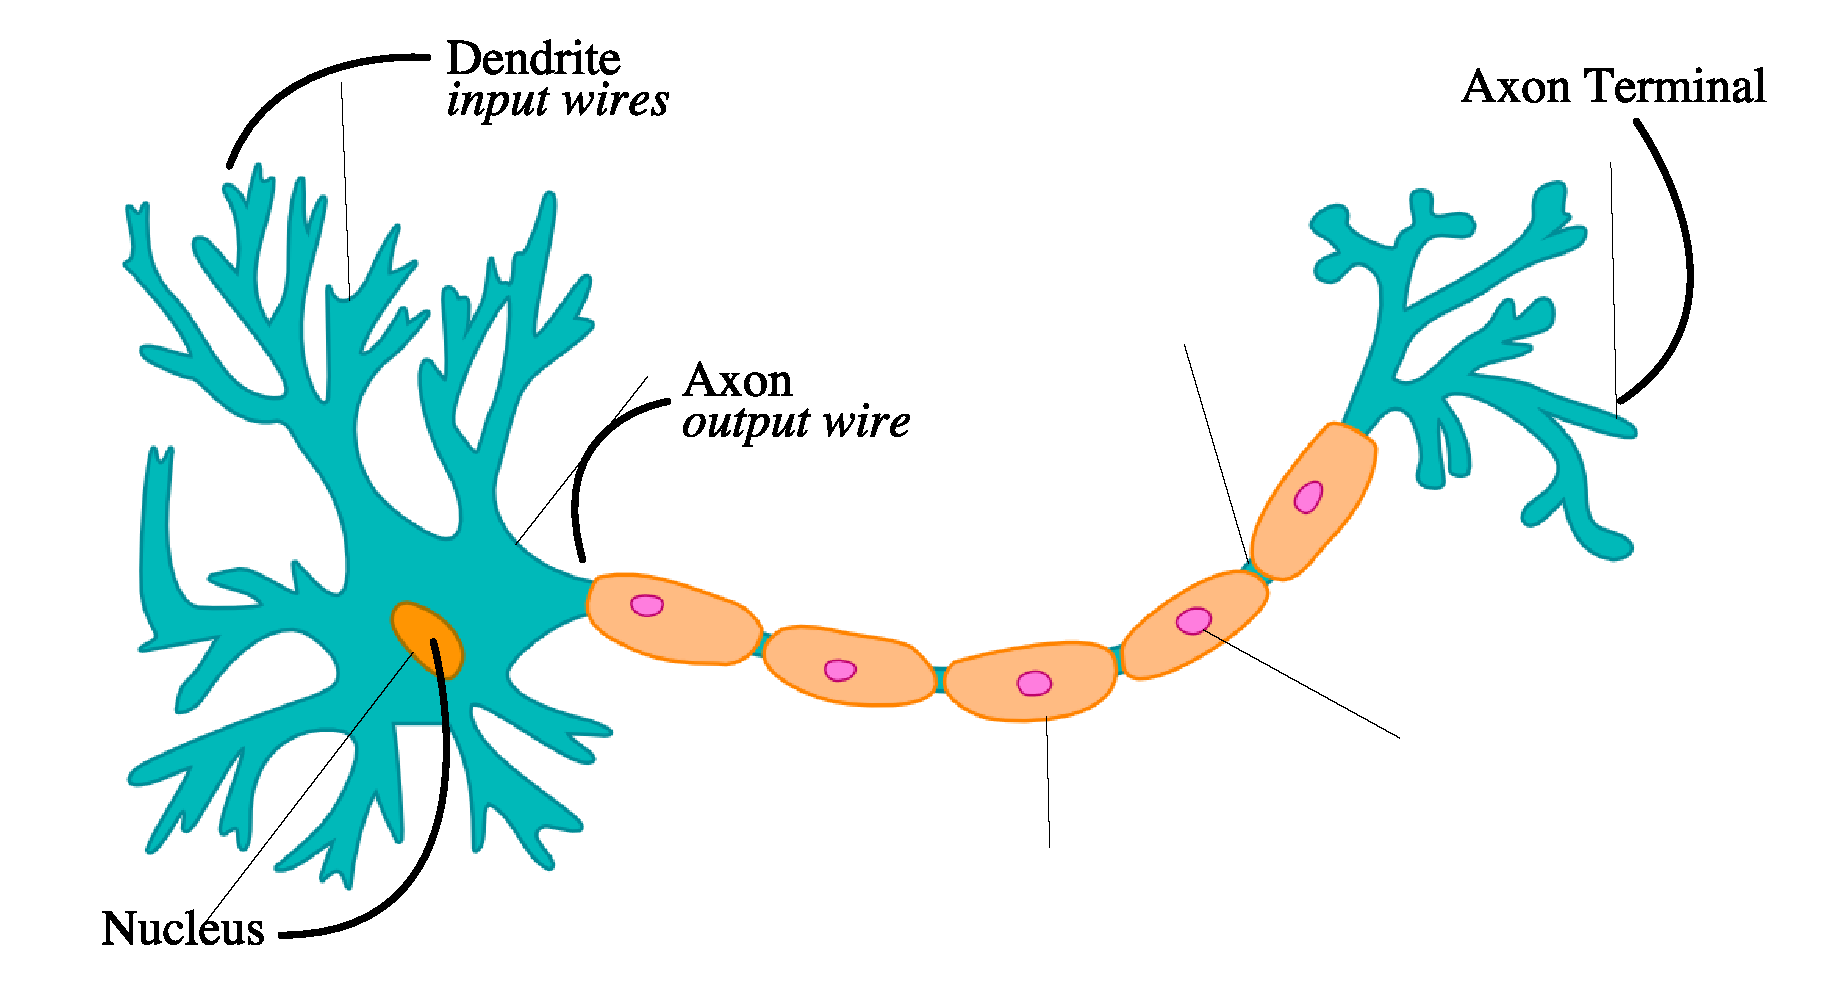
\includegraphics[scale = .4]{img/Neuron.pdf}
\caption[Structure of a Typical Biological Neuron]{Structure of a Typical Biological Neuron.\protect\footnotemark}
\label{fig:neuron}
\end{figure}

\footnotetext{Original SVG image by Quasar Jarosz but colors and some labels were modified for this paper.}

Figure \ref{fig:neuron} shows the typical nerve cell in Biology. In relation to the perceptron, the dendrite in this case takes several binary inputs and returns a single binary output on its axon. Mathematically, let $w_1,w_2,\cdots,w_p$ be the parameters or weights, and $x_1,x_2,\cdots, x_p$ be the inputs. Then the perceptron is defined as follows:

\begin{equation}
\label{eq:perceptron}
\begin{aligned}
y&=
\begin{cases}
0,& \sum_{i}w_i x_i\leq c\\
1,& \sum_{i}w_i x_i> c,
\end{cases}
\end{aligned}
\end{equation}

where $c$ is a threshold set by the experimenter. The following diagram in Figure \ref{fig:perceptron} is the schematic representation of Equation \ref{eq:perceptron}.

\begin{figure}[!t]
\vspace{0.7cm}
\centering\begin{tikzpicture}[
init/.style={
  draw,
  circle,
  inner sep=2pt,
  font=\Huge,
  join = by -latex
},
squa/.style={
  draw,
  inner sep=2pt,
  font=\Large,
  join = by -latex
},
start chain=4,node distance=13mm,thick
]
\begin{scope}[start chain=1]
\node[on chain=1] at (0,2.5cm) 
  (x1) {$x_1$};
\node[on chain=1,join=by o-latex] 
  (w1) {$w_1$};
\end{scope}

\begin{scope}[start chain=2]
\node[on chain=2] at (0,1.5cm) 
  (x2) {$x_2$};
\node[on chain=2,join=by o-latex] 
  (w2) {$w_2$};
\end{scope}

\begin{scope}[start chain=3, node distance = 18mm]
\node[on chain=3] at (0,.7cm) 
  {$\vdots$};
\node[on chain=3] at (0,.7cm) 
  {$\vdots$};
\end{scope}

\node[on chain=4] 
  (xi) {$x_i$};
\node[on chain=4,join=by o-latex] 
  (wi) {$w_i$};
\node[on chain=4,init] (sigma) 
  {$\displaystyle\Sigma$};
\node[on chain=4,label=above:Output,join=by -latex] 
  {$y$};

\begin{scope}[start chain=5,node distance=18mm]
\node[on chain=5] at (0,-.7cm) 
  {$\vdots$};
\node[on chain=5] at (0,-.7cm) 
  {$\vdots$};
\end{scope}

\begin{scope}[start chain=6]
\node[on chain=6] at (0,-1.5cm) 
  (xp) {$x_p$};
\node[on chain=6,label=below:Parameters,join=by o-latex] 
  (wp) {$w_p$};
\end{scope}


\draw[-latex] (w1) -- (sigma);
\draw[-latex] (w2) -- (sigma);
\draw[-latex] (wi) -- (sigma);
\draw[-latex] (wp) -- (sigma);

\draw[decorate,decoration={brace,mirror}] (x1.north west) -- node[left=10pt] {Inputs} (xp.south west);
\end{tikzpicture}
\vspace{0.7cm}
\caption[Schematic Representation of the Perceptron Neuron]{Schematic Representation of the Perceptron Neuron.}
\label{fig:perceptron}
\end{figure}
One limitation of the perceptron is its binary output, which sometimes is poor in discrimination problems, such as in text classification. To address this issue, a new artificial neuron is proposed that returns continuous values between 0 and 1, which can be interpreted as probabilities.

\section{Logistic Sigmoid Neuron}\label{sec:sln}
The logistic sigmoid neuron, or simply sigmoid neuron, takes its name from the fact that it uses the logistic function as its link/basis function; thus, it is also known as a logistic neuron. Formally, let $w_0$ be the intercept or the bias term and, as before, let $w_1,w_2,\cdots,w_p$ be the parameters. Then the logistic sigmoid function is given by
\begin{equation}\label{eq:logsig}
z=\sum_{i}w_ix_i+w_0,\quad y=\af(z)=\frac{1}{1+\exp(-z)}.
\end{equation}

In the following section, the connections between neurons will be discussed, as well as how the architecture of these networks is designed.

\section{Topology}\label{sec:topologyann}
The basic architecture of the network comprises the \textit{input} and the \textit{output} layers, between which are the \textit{hidden} layers. These hidden layers are layers that are not observed by the experimenter, hence the name. Figure \ref{fig:neuralnetarch} shows the diagram of a \textit{feedforward} neural network. It is feedforward due to the fact that the inputs are propagated onto the succeeding layers up to the output without redirecting back to the previous layer after processing. Otherwise, the model with recurrence would make it a \textit{recurrent} neural network.
\begin{figure}[!t]
\vspace{0.7cm}
\tikzset{%
  every neuron/.style={
    circle,
    draw,
    minimum size=.85cm
  },
  neuron missing/.style={
    draw=none, 
    scale=4,
    text height=0.333cm,
    execute at begin node=\color{black}$\vdots$
  },
}

\centering\begin{tikzpicture}[x=1.5cm, y=1.5cm, >=latex,thick]

\foreach \m/\l [count=\y] in {0,1,2,missing,3}
  \node [every neuron/.try, neuron \m/.try] (input-\m) at (0,2.5-\y) {};

\foreach \m [count=\y] in {0,1,missing,2}
  \node [every neuron/.try, neuron \m/.try ] (hidden-\m) at (2,2.6-\y*1.25) {};

\foreach \m [count=\y] in {1,missing,2}
  \node [every neuron/.try, neuron \m/.try ] (output-\m) at (4,1.5-\y) {};

\draw [<-] (input-0) -- ++(-1,0) node [above, midway] {$+1$};
\node [above] at (hidden-0.north) {$+1$};
\foreach \l [count=\i] in {1,2,p}
  \draw [<-] (input-\i) -- ++(-1,0)
    node [above, midway] {$x_{\l}$};

\foreach \i in {0,...,3}
  \foreach \j in {1,...,2}
    \draw [->] (input-\i) -- (hidden-\j);

\foreach \i in {0,...,2}
  \foreach \j in {1,...,2}
    \draw [->] (hidden-\i) -- (output-\j);

\foreach \l [count=\x from 0] in {Input, Hidden, Ouput}
  \node [align=center, above] at (\x*2,2) {\l \\ layer};

\end{tikzpicture}
\vspace{0.7cm}
\caption[Feedforward Neural Network]{Feedforward Neural Network.}
\label{fig:neuralnetarch}
\end{figure}
Since the input and output layers are observable, the hidden layers only serve as behind-the-scene computations. The parameters associated with each neuron have no interpretation at all, and that's one major limitation of ANNs. Neural networks can have several hidden layers depending on the study; for high levels of abstraction, one might consider multiple layers, also known as \textit{multilayer perceptrons} (MLP), which is a misnomer since these layers are made up of logistic sigmoid neurons, not of perceptrons. Networks with 2 or more hidden layers are often referred to as \textit{deep neural networks} \cite{nndeepl}, an example of which is depicted in Figure \ref{fig:deepnn}. The unknown vector $\mathbf{w}=[(w_i)]_{i=0}^p$ in Equation \ref{eq:logsig} is the parameter vector that needs to be estimated. This is done by maximum likelihood, which is equivalent to minimizing the error function through mathematical programming using methods such as the \textit{Gradient Descent} algorithm. The succeeding section will formalize the standard notations, then define the loss function which will be the basis for choosing the best estimates of the weights, and finally describe the estimation process.

\noindent
\begin{figure}[!b]
\vspace{0.7cm}
\tikzset{%
  every neuron/.style={
    circle,
    draw,
    minimum size=.85cm
  },
  neuron missing/.style={
    draw=none, 
    scale=4,
    text height=0.333cm,
    execute at begin node=\color{black}$\vdots$
  },
}
\centering\begin{tikzpicture}[x=1.31cm, y=1.5cm, >=latex,thick]

\foreach \m/\l [count=\y] in {1,2,3,missing,4}
  \node [every neuron/.try, neuron \m/.try] (input-\m) at (0,2-\y) {};

\foreach \m [count=\y] in {1,2,3,4,missing,5}
  \node [every neuron/.try, neuron \m/.try ] (hidden1-\m) at (2,2.5-\y) {};

\foreach \m [count=\y] in {1,2,missing,3}
  \node [every neuron/.try, neuron \m/.try ] (hidden2-\m) at (4,1.35-\y) {};

\foreach \m [count=\y] in {1,2,3,4,missing,5}
  \node [every neuron/.try, neuron \m/.try ] (hidden3-\m) at (6,2.5-\y) {};

\foreach \m [count=\y] in {1,missing,2}
  \node [every neuron/.try, neuron \m/.try ] (output-\m) at (8,1-\y) {};

\foreach \i in {1,...,4}
  \foreach \j in {1,2,3,4,...,5}
    \draw [->] (input-\i) -- (hidden1-\j);

\foreach \i in {1,2,3,4,...,5}
  \foreach \j in {1,2,...,3}
    \draw [->] (hidden1-\i) -- (hidden2-\j);

\foreach \i in {1,2,...,3}
  \foreach \j in {1,2,3,4,...,5}
    \draw [->] (hidden2-\i) -- (hidden3-\j);

\foreach \i in {1,2,3,4,...,5}
  \foreach \j in {1,...,2}
    \draw [->] (hidden3-\i) -- (output-\j);

\foreach \l [count=\x from 0] in {Input, Ouput}
  \node [align=center, above] at (\x*8,2) {\l \\ layer};

\draw (4,-4.7) node[above] {$\underbrace{\hspace{6cm}}_{\text{\small Hidden Layers}}$};
\end{tikzpicture}
\vspace{0.7cm}
\caption[Multilayer Feedforward Neural Network]{Multilayer Feedforward Neural Network.}
\label{fig:deepnn}
\end{figure}

\subsection{Notations}
The following definitions will serve as the standard notation for this appendix. To start with, let $f:\mathcal{X}\to\mathcal{Y}$ be the unknown \textit{target function} of the data points in the population, that is, $y:=f(\mathbf{x})$. The sample data set from this population is denoted by $(\mathbf{x}_1,y_1),\cdots,(\mathbf{x}_N,y_N)$. The learning algorithm picks $g:\mathcal{X}\to \mathcal{Y}$ as the \textit{final hypothesis} from the hypothesis set $\mathscr{H}:=\{h_v:h_v(\mathbf{x})=\hat{y},v\in\mathbb{N}\}$ s.t. $g\approx f$, that is, $g$ is the hypothesis that best approximates the target function $f$, thus $\hat{y}=g(\mathbf{x})$. The error in the training data set, named \textit{in-sample error}, is denoted by $\ein$, while the error in the validation dataset, named \textit{out-of-sample error}, is denoted by $\eout$.

For ANN models, let $i$, $j$, and $l$ be the indices of the observations in the inputs, outputs, and the layers containing the observations, respectively. The domains of these indices are as follows: $i\in\mathbb{N}_0^{(d^{(l-1)})}$, $j\in\mathbb{N}_1^{(d^{(l)})}$, and $l\in\mathbb{N}_1^L$, where $d^{(l)}$ is the dimension of the outputs in the $l$th layer. The upper bound of the inputs is $d^{(l-1)}$, since this is the dimension of the outputs in the previous layer, $l-1$, and is now an input layer due to the forward-propagation process; in this case, the next layer has $d^{(l)}$ dimension. Further, the lower bound of the input is 0 to account for the intercept term $w_0$. Hence, the standard notation for the parameters is $w_{ji}^{(l)}$.

Let $\mathbf{x}_k$ be the training input, $k\in\mathbb{N}$. Since the input layer is the $0$th layer with $d$ dimension, then each input is a $d^{(0)}\times 1$ vector. That is,
$$
\mathbf{x}_k=\left[
\begin{array}{c}
x_{k1}^{(0)}\\
x_{k2}^{(0)}\\
\vdots\\
x_{kd^{(0)}}^{(0)}
\end{array}
\right]
$$

In this setting, $h(\mathbf{x}_k,\mathbf{w})$ denotes the hypothesis or the model, where $\mathbf{w}$ is the vector of all weights. The feedforward process works as follows: the vector $\mathbf{x}_k$ will serve as an input on the first hidden layer, whose output will then be the input on the next hidden layer, and so on until the output layer. In general,
$$
x_{kj}^{(l)}=\af\left(z_{kj}^{(l)}\right)=\af\left(\left(\mathbf{w}_{j}^{(l)}\right)^{\top}\mathbf{x}_k^{(l-1)} + w_{j0}^{(l)}\right)=\af\left(\sum_{i=1}^{d^{(l-1)}}w_{ji}^{(l)}x_{ki}^{(l-1)}+w_{j0}^{(l)}\right),
$$
where $\mathbf{w}_{j}^{(l)}=\left[\begin{array}{cccc}w_{j1}^{(1)}&w_{j2}^{(2)}&\cdots&w_{jd^{(l-1)}}^{(l)}\end{array}\right]^{\top}$. This computation is propagated up to the output layer. For example, the following is the formula for obtaining $x_{kj}^{(l+1)}$:
$$
\begin{aligned}
x_{kj}^{(l+1)}&=\af\left(z_{kj}^{(l+1)}\right)=\af\left(\left(\mathbf{w}_{j}^{(l+1)}\right)^{\top}\mathbf{x}_k^{(l)} + w_{j0}^{(l+1)}\right)=\af\left(\sum_{i=1}^{d^{(l)}}w_{ji}^{(l+1)}x_{ki}^{(l)}+w_{j0}^{(l+1)}\right)\\
&=\af\left\{\sum_{i=1}^{d^{(l)}}w_{ji}^{(l+1)}\left[\af\left(\sum_{i=1}^{d^{(l-1)}}w_{ji}^{(l)}x_{ki}^{(l-1)}+w_{j0}^{(l)}\right)\right]+w_{j0}^{(l+1)}\right\}.
\end{aligned}
$$
So the dimension $d$ will vary from layer to layer. Consider Figure \ref{fig:neuralnetarch}; the neurons can now be labeled with the standard notations as in Figure \ref{fig:nnlab}.
Thus, $x_{kj}^{(1)}$ in the hidden layer has the following form:
$$
x_{kj}^{(1)}=\af(z_{kj}^{(1)})=\af\left(\left(\mathbf{w}_{j}^{(1)}\right)^{\top}\mathbf{x}_k^{(0)} + w_{j0}^{(1)}\right)=\af\left(\sum_{i=1}^{d^{(0)}}w_{ji}^{(1)}x_{ki}^{(0)}+w_{j0}^{(1)}\right),
$$
The $x_{kj}^{(2)}$ in the output layer is computed from the following equation:
$$
\begin{aligned}
x_{kj}^{(2)}&=\af(z_{kj}^{(2)})=\af\left(\left(\mathbf{w}_{j}^{(2)}\right)^{\top}\mathbf{x}_k^{(1)} + w_{j0}^{(2)}\right)=\af\left(\sum_{i=1}^{d^{(1)}}w_{ji}^{(2)}x_{ki}^{(1)}+w_{j0}^{(2)}\right)\\
&=\af\left\{\sum_{i=1}^{d^{(1)}}w_{ji}^{(2)}\left[\af\left(\sum_{i=1}^{d^{(0)}}w_{ji}^{(1)}x_{ki}^{(0)}+w_{j0}^{(1)}\right)\right]+w_{j0}^{(2)}\right\}.
\end{aligned}
$$

\begin{figure}[!t]
\vspace{0.7cm}
\tikzset{%
  every neuron/.style={
    circle,
    draw,
    minimum size=.85cm
  },
  neuron missing/.style={
    draw=none, 
    scale=4,
    text height=0.333cm,
    execute at begin node=\color{black}$\vdots$
  },
}

\centering\begin{tikzpicture}[x=1.5cm, y=1.5cm, >=latex, thick]

\foreach \m/\l [count=\y] in {0,1,2,missing,3}
  \node [every neuron/.try, neuron \m/.try] (input-\m) at (0,2.5-\y) {};

\foreach \m [count=\y] in {0,1,missing,2}
  \node [every neuron/.try, neuron \m/.try ] (hidden-\m) at (2,2.6-\y*1.25) {};

\foreach \m [count=\y] in {1,missing,2}
  \node [every neuron/.try, neuron \m/.try ] (output-\m) at (4,1.5-\y) {};

  \draw [<-] (input-0) -- ++(-1,0) node [above, midway] {$+1$};
\foreach \l [count=\i] in {1,2,d^{(0)}}
  \draw [<-] (input-\i) -- ++(-1,0)
    node [above, midway] {$x_{k\l}^{(0)}$};

%\foreach \l [count=\i] in {1,missing}
  \node [above] at (hidden-0.north) {$+1$};
  \node [above] at (hidden-1.north) {$x_{k1}^{(1)}$};
  \node [below] at (hidden-2.south) {$x_{kd^{(1)}}^{(1)}$};

\foreach \l [count=\i] in {1,d^{(2)}}
  \draw [->] (output-\i) -- ++(1,0)
    node [above, midway] {$x_{k\l}^{(2)}$};

\foreach \i in {0,...,3}
  \foreach \j in {1,...,2}
    \draw [->] (input-\i) -- (hidden-\j);

\foreach \i in {0,...,2}
  \foreach \j in {1,...,2}
    \draw [->] (hidden-\i) -- (output-\j);

\foreach \l [count=\x from 0] in {Input, Hidden, Ouput}
  \node [align=center, above] at (\x*2,2) {\l \\ layer};

\end{tikzpicture}
\vspace{0.7cm}
\caption[Neural Net with Standard Neuron Notation]{Neural Net with Standard Neuron Notation.}
\label{fig:nnlab}
\end{figure}

The final output $\mathbf{x}_{k}^{(2)}$ is the value of the hypothesis, that is, $h(\mathbf{x}_k,\mathbf{w})=\mathbf{x}_{k}^{(L)}$, where $L=2$.

\section{Network Training}
The nonlinearity of the loss function of a neural network makes it hard to compute the weights analytically, and instead the approach is often through numerical approximation.

\subsection{Loss Function}\label{sec:costfun}
In this section, the error functions of ANN models for regression and classification are derived from a probabilistic perspective. For the regression setup, the network has at least two nodes (one for the intercept and one for the independent variable) at the input layer and one node at the output layer. The standard activation function is the identity function, i.e., $h(\mathbf{x}_k,\mathbf{w})=z_k=\mathbf{w}^{\top}\mathbf{x}_k$, so there is no hidden layer; see Figure \ref{fig:slrnn}.
\begin{figure}[!t]
\vspace{0.7cm}
\centering\begin{tikzpicture}[
init/.style={
  draw,
  circle,
  inner sep=2pt,
  font=\Huge,
  join = by -latex
},
squa/.style={
  draw,
  inner sep=2pt,
  font=\Large,
  join = by -latex
},
start chain=4,node distance=13mm, thick
]
\begin{scope}[start chain=1]
\node[on chain=1] at (0,2.5cm) 
  (x1) {$x_{k1}^{(0)}$};
\node[on chain=1,join=by o-latex] 
  (w1) {$w_{11}^{(1)}$};
\end{scope}

\begin{scope}[start chain=2]
\node[on chain=2] at (0,1.5cm) 
  (x2) {$x_{k2}^{(0)}$};
\node[on chain=2,join=by o-latex] 
  (w2) {$w_{12}^{(1)}$};
\end{scope}

\begin{scope}[start chain=3, node distance = 20mm]
\node[on chain=3] at (0,.7cm) 
  {$\vdots$};
\node[on chain=3] at (0,.7cm) 
  {$\vdots$};
\end{scope}

\node[on chain=4] 
  (xi) {$x_{ki}^{(0)}$};
\node[on chain=4,join=by o-latex] 
  (wi) {$w_{1i}^{(1)}$};
\node[on chain=4,init] (sigma) 
  {$\displaystyle\Sigma$};
\node[on chain=4,label=above:Output,join=by -latex] 
  {$h(\mathbf{x},\mathbf{w})$};

\begin{scope}[start chain=5,node distance=20mm]
\node[on chain=5] at (0,-.7cm) 
  {$\vdots$};
\node[on chain=5] at (0,-.7cm) 
  {$\vdots$};
\end{scope}

\begin{scope}[start chain=6]
\node[on chain=6] at (0,-1.5cm) 
  (xp) {$x_{kd^{(0)}}^{(0)}$};
\node[on chain=6,label=below:Parameters,join=by o-latex] 
  (wp) {$w_{1d^{(0)}}^{(1)}$};
\end{scope}

\node[label=above:\parbox{2cm}{\centering Intercept \\ $w_0$}] at (sigma|-w2) (b) {};

\draw[-latex] (w1) -- (sigma);
\draw[-latex] (w2) -- (sigma);
\draw[-latex] (wi) -- (sigma);
\draw[-latex] (wp) -- (sigma);
\draw[o-latex] (b) -- (sigma);

\end{tikzpicture}
\vspace{0.7cm}
\caption[Neuron's Schematic Diagram for Linear Regression]{Neuron's Schematic Diagram for Linear Regression.}
\label{fig:slrnn}
\end{figure}
Given the training input $\mathbf{X}:=[\mathbf{x}_1^{(0)},\mathbf{x}_2^{(0)},\cdots,\mathbf{x}_N^{(0)}]$, where $\mathbf{x}_k^{(0)}$ is a $d^{(0)}$-dimensional feature vector whose elements are $\left[x_{k0}^{(0)},x_{k1}^{(0)},\cdots, x_{kd^{(0)}}^{(0)}\right]^{\top}\;\forall k\in\mathbb{N}$, the corresponding target variable is $\mathbf{Y}:=[y_1,y_2,\cdots,y_N]^{\top}$, and the error term $\varepsilon_k$ is assumed to be normally distributed with mean $\ev\varepsilon_k=0$ and variance $\var\varepsilon_k=\sigma^2$. It follows that the uncertainty around the target variable is also Gaussian distributed and is given by
\begin{align}
p(y|\mathbf{x},\mathbf{w},\sigma^2)&=\mathcal{N}(y|h(\mathbf{x},\mathbf{w}),\sigma^2)\nonumber\\
&:=\frac{1}{\sqrt{2\pi\sigma^{2}}}\exp\left[-\frac{(y-h(\mathbf{x},\mathbf{w}))^2}{2\sigma^{2}}\right].
\end{align}
If the data are independent and identically distributed, then the likelihood function of $\mathbf{y}$ is given by
\begin{align}
\mathcal{L}(\mathbf{w},\sigma|\mathbf{y},\mathbf{X})&=p(\mathbf{y}|\mathbf{X},\mathbf{w},\sigma)=\prod_{k=1}^{K}\mathcal{N}(y_k|h(\mathbf{x}_k,\mathbf{w}),\sigma^2)\nonumber\\
&=\frac{1}{(2\pi)^{K/2}\sigma^K}\exp\left[-\frac{1}{2\sigma^2}\sum_{k=1}^{K}(y_k-h(\mathbf{x}_k,\mathbf{w}))^2\right].
\end{align}
Taking the log-likelihood,
\begin{equation}
\label{eq:mle}
\ell(\mathbf{w},\sigma|\mathbf{y},\mathbf{X})=-\frac{1}{2\sigma^2}\sum_{k=1}^K(y_k-h(\mathbf{x}_k,\mathbf{w}))^2-K\log\sigma-\frac{K}{2}\log 2\pi.
\end{equation}
The estimate for the weight $\mathbf{w}$, denoted by $\hat{\mathbf{w}}_{\mathrm{MLE}}$, is obtained by maximizing the log-likelihood function. To do so, partial differentiation is applied to Equation \ref{eq:mle} with respect to $\mathbf{w}$, suggesting that the last two terms on the right-hand side can be disregarded since these are not dependent on $\mathbf{w}$. Also, the location of the maximum log-likelihood with respect to $\mathbf{w}$ is not affected by arbitrary positive scalar multiplication, so the factor $\frac{1}{\sigma^2}$ can be omitted. Equivalently, one can minimize the negative log-likelihood instead of maximizing $\ell$. The reason for doing this has to do with numerical computation, since optimizers in most statistical packages often work by minimizing the function. Thus, differentiating the negative of Equation \ref{eq:mle} is the same as differentiating the following equation:
\begin{equation}
\label{eq:regin}
\ein(h)=\frac{1}{2}\sum_{k=1}^K(y_k-h(\mathbf{x}_k,\mathbf{w}))^2,
\end{equation}
which is similar to the form of the \textit{residual sum-of-squares}. Hence, the sum-of-squares error function is a consequence of maximum likelihood under the normality assumption of the uncertainty around the target variable.

Likewise, the precision parameter can be estimated using maximum likelihood by simply differentiating Equation \ref{eq:mle} with respect to $\sigma$, i.e.,
$$
\hat{\sigma}_{\mathrm{mle}}^2=\frac{1}{K}\sum_{k=1}^K(y_k-h(\mathbf{x}_k,\mathbf{w}))^2.
$$

Now consider the case for classification, in which there is a single target variable $y$ that returns binary output, where $y=1$ corresponds to class $\mathcal{C}_1$ and $y=0$ to class $\mathcal{C}_2$. The appropriate activation function is the logistic sigmoid defined in Section \ref{sec:sln}, that is, 
$$
\af(z)=\frac{1}{1+\exp(-z_k)},
$$
implying $\af:\mathbb{R}\to[0,1]$, and hence it can be interpreted as a probability. This type of model has the same network architecture and neuron's schematic diagram as that in the linear regression model (see Figure \ref{fig:slrnn}), but this time the activation function has a unit interval range with hypothesis given by
$$\hat{y}=h(\mathbf{x},\mathbf{w})=\begin{cases}
1,&\af>c\\
0,&\af\leq c
\end{cases},$$
where $c$ is specified by the user and is often chosen to be 0.5.

\begin{figure}[t]
  \vspace{0.7cm}
\centering\begin{tikzpicture}[
init/.style={
  draw,
  circle,
  inner sep=2pt,
  font=\Huge,
  join = by -latex
},
squa/.style={
  draw,
  inner sep=2pt,
  font=\Large,
  join = by -latex
},
squa1/.style={
  draw,
  inner sep=2pt,
  join = by -latex
},
start chain=4,node distance=13mm, thick
]
\begin{scope}[start chain=1]
\node[on chain=1] at (0,2.5cm) 
  (x1) {$x_{k1}^{(0)}$};
\node[on chain=1,join=by o-latex] 
  (w1) {$w_{11}^{(1)}$};
\end{scope}

\begin{scope}[start chain=2]
\node[on chain=2] at (0,1.5cm) 
  (x2) {$x_{k2}^{(0)}$};
\node[on chain=2,join=by o-latex] 
  (w2) {$w_{12}^{(1)}$};

\end{scope}

\begin{scope}[start chain=3, node distance = 20mm]
\node[on chain=3] at (0,.7cm) 
  {$\vdots$};
\node[on chain=3] at (0,.7cm) 
  {$\vdots$};
\end{scope}

\node[on chain=4] 
  (xi) {$x_{ki}^{(0)}$};
\node[on chain=4,join=by o-latex] 
  (wi) {$w_{1i}^{(1)}$};
\node[on chain=4,init] (sigma) 
  {$\displaystyle\Sigma$};
\node[on chain=4,squa,label=above:{\parbox{2cm}{\centering Activation \\ function}}]   
  (af) {$\af$};
\node[on chain=4,squa1]
  (con) {if $\af>c$};

\begin{scope}[start chain=5,node distance=20mm]
\node[on chain=5] at (0,-.7cm) 
  {$\vdots$};
\node[on chain=5] at (0,-.7cm) 
  {$\vdots$};
\end{scope}

\begin{scope}[start chain=6]
\node[on chain=6] at (0,-1.5cm) 
  (xp) {$x_{kd^{(0)}}^{(0)}$};
\node[on chain=6,label=below:Parameters,join=by o-latex] 
  (wp) {$w_{1d^{(0)}}^{(1)}$};
\end{scope}

\node[label=above:\parbox{2cm}{\centering Intercept \\ $w_0$}] at (sigma|-w1) (b) {};
\node at (9.5,1.6cm) {True};
\node at (11.5,1.3cm) (tr) {$\hat{y}=1$};
\node at (11.5,-1.3cm) (fl) {$\hat{y}=0$};
\node at (9.5,-1.6cm) {False};
\draw[-latex] (w1) -- (sigma);
\draw[-latex] (w2) -- (sigma);
\draw[-latex] (wi) -- (sigma);
\draw[-latex] (wp) -- (sigma);
\draw[o-latex] (b) -- (sigma);
\draw[-latex] (con) |- (tr);
\draw[-latex] (con) |- (fl);

\end{tikzpicture}
\vspace{0.7cm}
\caption[Neuron's Schematic Diagram for Logistic Regression]{Neuron's Schematic Diagram for Logistic Regression.}
\label{fig:logrnn}
\end{figure}
The probability of success, in this case $y=1$ for $\mathcal{C}_1$, is 
$$
p(y=1|h(\mathbf{x},\mathbf{w}))=h(\mathbf{x},\mathbf{w})
$$
Thus, the conditional distribution of the target variable $y$ given $\mathbf{x}$ is a Bernoulli distribution with density given by
$$
p(y|h(\mathbf{x},\mathbf{w}))=\mathcal{B}(y|h(\mathbf{x},\mathbf{w}))=h(\mathbf{x},\mathbf{w})^{y}(1-h(\mathbf{x},\mathbf{w}))^{1-y},\quad y\in\{0,1\}.
$$

For a sample data set $\{\mathbf{x}_k,y_k\}$ where $\mathbf{x}_k$ is a $d^{(0)}$-dimensional feature vector and $y_k\in\{0,1\}\;\forall k\in\mathbb{N}$, if the $y$s are independent and identically distributed, then the likelihood function is given by
$$
\mathcal{L}(h(\mathbf{x}_k,\mathbf{w})|\mathbf{y})=\prod_{k=1}^{K}h(\mathbf{x}_k,\mathbf{w})^{y_k}(1-h(\mathbf{x}_k,\mathbf{w}))^{1-y_k},
$$
and the negative log-likelihood is given by 
\begin{align}
\ein(h)&=-\ell (h(\mathbf{x}_k,\mathbf{w})|\mathbf{y})\nonumber\\
&=-\sum_{k=1}^{K}\left[y_k\log h(\mathbf{x}_k,\mathbf{w})+(1-y_k)\log(1-h(\mathbf{x}_k,\mathbf{w}))\right].\label{eq:logitein}
\end{align}
This equation is known as the \textit{cross-entropy} loss function.
\begin{figure}[!t]
  \vspace{0.7cm}
\centering
\tikzset{%
  every neuron/.style={
    circle,
    draw,
    minimum size=.85cm
  },
  neuron missing/.style={
    draw=none, 
    scale=4,
    text height=0.333cm,
    execute at begin node=\color{black}$\vdots$
  },
}
\centering\begin{tikzpicture}[x=1.1cm, y=1.5cm, >=latex, thick]

\foreach \m/\l [count=\y] in {1,2,missing,3}
  \node [every neuron/.try, neuron \m/.try] (input-\m) at (0,1-\y) {};

\foreach \m [count=\y] in {1,missing,2}
  \node [every neuron/.try, neuron \m/.try ] (output-\m) at (2,.5-\y) {};

\foreach \l [count=\i+1] in {0,1,d^{(0)}}
  \draw [<-] (input-\i) -- ++(-1,0)
    node [above, midway] {$x_{k\l}^{(0)}$};

\foreach \l [count=\i] in {1,d^{(1)}}
  \draw [->] (output-\i) -- ++(1,0)
    node [above, right] {$x_{k\l}^{(1)}=y_k\in\{0,1\}$};

\foreach \i in {1,2,...,3}
  \foreach \j in {1,...,2}
    \draw [->] (input-\i) -- (output-\j);
\end{tikzpicture}
\vspace{0.7cm}
\caption[Neural Network for $d^{(1)}\geq 2$ Output Nodes]{Neural Network for $d^{(1)}\geq 2$ Output Nodes}
\label{fig:kloginn}
\end{figure}
Extending the case to at least two separate binary classifications requires $d^{(L)}\geq 2$ neurons on the output layer, each of which has a logistic sigmoid activation function. The target variable is defined as $\mathbf{y}_k=[y_1,y_2,\cdots,y_{d^{(L)}}]^{\top}$, where $y_j\in\{0,1\}\;\forall j\in\mathbb{N}^{(L)}$. Assuming independence of the class labels, the joint conditional distribution of the targets given the input vector is
$$
p(\mathbf{y}|\mathbf{x},\mathbf{w})=\prod_{j=1}^{d^{(L)}}h(\mathbf{x},\mathbf{w})^{y_j}\left[1-h(\mathbf{x},\mathbf{w})\right]^{1-y_j}.
$$
Then the likelihood function is given by
$$
\mathcal{L}(h(\mathbf{x}_k,\mathbf{w})|\mathbf{y})=\prod_{k=1}^{K}\prod_{j=1}^{d^{(L)}}h(\mathbf{x}_{k},\mathbf{w})^{y_{kj}}\left[1-h(\mathbf{x}_{k},\mathbf{w})\right]^{1-y_{kj}}.
$$
The negative log-likelihood then becomes
\begin{align}
\ein(h)&=-\ell (h(\mathbf{x}_{k},\mathbf{w})|\mathbf{y})\nonumber\\
&=-\sum_{k=1}^{K}\sum_{j=1}^{d^{(L)}}\left[y_{kj}\log h(\mathbf{x}_{k},\mathbf{w})+(1-y_{kj})\log(1-h(\mathbf{x}_{k},\mathbf{w}))\right].\label{eq:mlogitein}
\end{align}

In general, the loss function of a neural network can be written as the average of the errors in the output layer across all $k$ training inputs, i.e.,
\begin{align}
\ein(h)&=\frac{1}{K}\sum_{k=1}^K\frac{1}{2}\sum_{j=1}^{d^{(L)}}(y_{kj}-h(\mathbf{x}_{k},\mathbf{w}))^2\\
&=\frac{1}{K}\sum_{k=1}^K\varepsilon(h(\mathbf{x}_{k},\mathbf{w}),y_{kj})
\end{align}

This equation is also known as the \textit{mean squared error}. In order to minimize this function, one has to consider numerical methods such as \textit{gradient descent} or \textit{stochastic gradient descent}.

\subsection{Back-propagation Algorithm}\label{sec:backprop}
The average error of the $k$ training inputs defined in Section \ref{sec:costfun} is given by
\begin{equation}\label{eq:errornn}
\ein(\mathbf{w}):=\frac{1}{K}\sum_{k=1}^{K}\varepsilon(\mathbf{h}(\mathbf{x}_k,\mathbf{w}),\mathbf{y}_k).
\end{equation}
The terms in this equation are errors of the training inputs. That is, for each training input, there is a corresponding error that needs to be minimized. This error is the difference between the target $\mathbf{y}_k$ and the output of the hypothesis $\mathbf{h}(\mathbf{x}_k,\mathbf{w})$. To account for the iteration counter $r$, let $\hat{\mathbf{w}}_r$ be the notation for the estimate of $\mathbf{w}$ at the $r$th iteration; also let $\varepsilon_r$ be the error of the $r$th iteration. The inner term of Equation \ref{eq:errornn} can be expanded as follows:
\begin{align}
\varepsilon(\mathbf{h}(\mathbf{x}_k,\hat{\mathbf{w}}_r),\mathbf{y}_k)&:=\frac{1}{2}\lVert\mathbf{y}_k-\mathbf{h}(\mathbf{x}_k,\hat{\mathbf{w}}_r)\rVert^2=\frac{1}{2}\sum_{j=1}^{d^{(L)}}(y_{kj}-h_j(\mathbf{x}_k,\mathbf{w}))^2\nonumber\\
&=\frac{1}{2}\sum_{j=1}^{d^{(L)}}\left(y_{kj}-x_{kj}^{(L)}\right)^2=\frac{1}{2}\sum_{j=1}^{d^{(L)}}\left[y_{kj}-\af\left(z_{kj}^{(L)}\right)\right]^2\nonumber\\
&=\frac{1}{2}\sum_{j=1}^{d^{(L)}}\left[y_{kj}-\af\left(\sum_{i=1}^{d^{(L-1)}}w_{ji}^{(L)}x_{ki}^{(L-1)}+w_{j0}^{(L)}\right)\right]^2.
\end{align}
For each training input $k$, the gradient descent algorithm is applied to the function $\varepsilon(\mathbf{h}(\mathbf{x}_k,\mathbf{w}),\mathbf{y}_{k})$. The average of all these functions corresponds to the loss function, so the minimum average of the error terms will give the corresponding estimate of the parameters. For simplicity, assume there is only one hidden layer, that is, $L=2$. Consider the following:

\begin{equation}
\frac{\partial \ein(\mathbf{w})}{\partial w_{ji}^{(L)}}=\frac{\partial \ein(\mathbf{w})}{\partial \varepsilon(\mathbf{h}(\mathbf{x}_k,\mathbf{w}),\mathbf{y}_{k})}\frac{\partial \varepsilon(\mathbf{h}(\mathbf{x}_k,\mathbf{w}),\mathbf{y}_{k})}{\partial w_{ji}^{(L)}}
\end{equation}
where,
\begin{align}
\frac{\partial \ein(\mathbf{w})}{\partial \varepsilon(\mathbf{h}(\mathbf{x}_k,\mathbf{w}),\mathbf{y}_{k})}&=\frac{\partial}{\partial \varepsilon(\mathbf{h}(\mathbf{x}_k,\mathbf{w}),\mathbf{y}_{k})}\frac{1}{K}\sum_{k=1}^{K}\varepsilon(\mathbf{h}(\mathbf{x}_k,\mathbf{w}),\mathbf{y}_k)\nonumber\\
&=\frac{1}{K}\sum_{k=1}^{K}\frac{\partial}{\partial \varepsilon(\mathbf{h}(\mathbf{x}_k,\mathbf{w}),\mathbf{y}_{k})}\frac{1}{2}\sum_{j=1}^{d^{(L)}}(y_{kj}-h_j(\mathbf{x}_k,\mathbf{w}))^2\nonumber\\
&=\frac{1}{K}\sum_{k=1}^{K}\frac{\partial}{\partial \varepsilon(\mathbf{h}(\mathbf{x}_k,\mathbf{w}),\mathbf{y}_{k})}\frac{1}{2}\sum_{j=1}^{d^{(L)}}\left[y_{kj}-x_{kj}^{(L)}\right]^2\nonumber\\
&=\frac{1}{K}\sum_{k=1}^{K}\sum_{j=1}^{d^{(L)}}\left[y_{kj}-x_{kj}^{(L)}\right],\label{eq:err}
\end{align}
and
\begin{align}
\frac{\partial \varepsilon(\mathbf{h}(\mathbf{x}_k,\mathbf{w}),\mathbf{y}_{k})}{\partial w_{ji}^{(L)}}&=\frac{\partial}{\partial w_{ji}^{(L)}}\frac{1}{K}\sum_{k=1}^{K}\sum_{j=1}^{d^{(L)}}\left[y_{kj}-x_{kj}^{(L)}\right]\nonumber\\
&=\frac{1}{K}\sum_{k=1}^{K}\left[-\left(y_{kj}-x_{kj}^{(L)}\right)\frac{\partial x_{kj}^{(L)}}{\partial w_{ji}^{(L)}}\right].\label{eq:inerr}
\end{align}
And note that, $x_{kj}^{(L)}=\af\!\left(z_{kj}^{(L)}\right)=\af\!\left(\sum_{i=1}^{d^{(L-1)}}w_{ji}^{(L)}x_{ki}^{(L-1)}+w_{j0}^{(L)}\right)$. Hence,
\begin{align}
\frac{\partial \ein(\mathbf{w})}{\partial w_{ji}^{(L)}}&=-\frac{1}{K}\sum_{k=1}^{K}\left(y_{kj}-x_{kj}^{(L)}\right)\frac{\partial x_{kj}^{(L)}}{\partial z_{kj}^{(L)}}\frac{\partial z_{kj}^{(L)}}{\partial w_{ji}^{(L)}}\nonumber\\
&=-\frac{1}{K}\sum_{k=1}^{K}\left(y_{kj}-x_{kj}^{(L)}\right)\af'\!\left(z_{kj}^{(L)}\right)x_{ki}^{(L-1)}.\label{eq:grad1}
\end{align}
A gradient descent update at the $(r+1)$st iteration has the form,
\begin{equation}
w_{ji,r+1}^{(L)}=w_{ji,r}^{(L)}+\Delta w_{ji,r}^{(L)}=w_{ji,r}^{(L)}-\gamma\frac{\partial \ein(h)}{\partial w_{ji,r}^{(L)}}.
\end{equation}
The $\Delta w_{ji,r}^{(L)}$ can be expressed as follows:
\begin{equation}
\Delta w_{ji,r}^{(L)}=-\gamma\frac{\partial \ein(h)}{\partial w_{ji,r}^{(L)}}=\gamma\delta_{j}^{(L)}x_{ki}^{(L-1)},
\end{equation}
where $\delta_{j}^{(L)}$ is the \textit{local gradient} defined as
\begin{align}
\delta_{j}^{(L)}&=-\frac{\partial \ein(h)}{\partial z_{kj}^{(L)}}=-\frac{\partial \ein(h)}{\partial x_{kj}^{(L)}}\frac{\partial x_{kj}^{(L)}}{\partial z_{kj}^{(L)}}=\frac{1}{K}\sum_{k=1}^{K}\varepsilon(h_j(\mathbf{x}_k,\mathbf{w}),y_{kj})\af'\!\left(z_{kj}^{(L)}\right)\nonumber\\
&=\frac{1}{K}\sum_{k=1}^{K}\left(y_{kj}-x_{kj}^{(L)}\right)\af'\!\left(z_{kj}^{(L)}\right).
\end{align}
Thus, the local gradient is the product of the error signal at the $j$th neuron of the $L$th layer and the derivative of the associated activation function.

For weights at the $(L-1)$th layer, the local gradient is then given by
\begin{equation}\label{eq:delta2}
\delta_{j}^{(L-1)}=-\frac{\partial \mathcal{E}_{in}(\mathbf{w})}{\partial x_{kj}^{(L-1)}}\frac{\partial x_{kj}^{(L-1)}}{\partial z_{kj}^{(L-1)}}=-\frac{\partial \mathcal{E}_{in}(\mathbf{w})}{\partial x_{kj}^{(L-1)}}\af'\!\left(z_{kj}^{(L-1)}\right).
\end{equation}
where
\begin{equation}
\frac{\partial \mathcal{E}_{in}(\mathbf{w})}{\partial x_{kj}^{(L-1)}}=\frac{\partial \mathcal{E}_{in}(\mathbf{w})}{\partial \varepsilon(\mathbf{h}(\mathbf{x}_k,\mathbf{w}),\mathbf{y}_{k})}\frac{\partial \varepsilon(\mathbf{h}(\mathbf{x}_k,\mathbf{w}),\mathbf{y}_{k})}{\partial x_{kj}^{(L)}}\frac{\partial x_{kj}^{(L)}}{\partial z_{kj}^{(L)}}\frac{\partial z_{kj}^{(L)}}{\partial x_{kj}^{(L-1)}}.
\end{equation}
And since
\begin{equation}
\frac{\partial \mathcal{E}_{in}(\mathbf{w})}{\partial \varepsilon(\mathbf{h}(\mathbf{x}_k,\mathbf{w}),\mathbf{y}_{k})}\frac{\partial \varepsilon(\mathbf{h}(\mathbf{x}_k,\mathbf{w}),\mathbf{y}_{k})}{\partial x_{kj}^{(L)}}=-\frac{1}{K}\sum_{k=1}^{K}\sum_{j=1}^{d^{(L)}}\left(y_{kj}-x_{kj}^{(L)}\right)
\end{equation}
then
\begin{align}
\frac{\partial \mathcal{E}_{in}(\mathbf{w})}{\partial x_{kj}^{(L-1)}}&=-\frac{1}{K}\sum_{k=1}^{K}\sum_{j=1}^{d^{(L)}}\left(y_{kj}-x_{kj}^{(L)}\right)\frac{\partial x_{kj}^{(L)}}{\partial z_{kj}^{(L)}}\frac{\partial z_{kj}^{(L)}}{\partial x_{kj}^{(L-1)}}\nonumber\\
&=-\sum_{j=1}^{d^{(L)}}\frac{1}{K}\sum_{k=1}^{K}\left(y_{kj}-x_{kj}^{(L)}\right)\af'\!\left(z_{kj}^{(L)}\right)w_{ji}^{(L)}\nonumber\\
&=-\sum_{j=1}^{d^{(L)}}\delta_j^{(L)}w_{ji}^{(L)}.\label{eq:deltawij}
\end{align}
So that using Equation \ref{eq:deltawij} in \ref{eq:delta2},
\begin{equation}\label{eq:backprop}
\delta_{i}^{(L-1)}=\af'\!\left(z_{ki}^{(L-1)}\right)\sum_{j=1}^{d^{(L)}}\delta_j^{(L)}w_{ji}^{(L)}.
\end{equation}
To emphasize, $\af'\!\left(z_{ki}^{(L-1)}\right)$ is indexed at $i$ but at the $(L-1)$th layer, so the dimension on that layer is not necessarily the same as the $L$th layer, and thus it is not included in the summation. Equation \ref{eq:backprop} is known as the \textit{back-propagation equation}.

\section{Transformers}\label{sec:transformers}
Transformer models are models based on the work of \cite{vaswani2017attention}. These models are a type of neural network architecture designed to handle sequential data, primarily used in natural language processing (NLP) tasks. Unlike traditional variants of ANN like Recurrent Neural Networks (RNNs) and Long Short-Term Memory (LSTM) networks, Transformers do not rely on sequential data processing. Instead, they utilize an \textit{attention} mechanism that allows them to process entire sequences simultaneously, significantly improving efficiency and effectiveness. The following formulation is based from \cite{bishop2023learning}.

\subsection{Attention Mechanism}\label{sec:attention-mechanism}
The core innovation of transformers is the self-attention mechanism, which computes attention scores to weigh the importance of different words in a sentence relative to each other. 

\begin{defn}[Vector Self-Attention]\label{defn:vec-self-attention}
    Let $\mathbf{X}:=[\mathbf{x}_1,\cdots,\mathbf{x}_N]^{\top}$ be the data matrix, s.t. $\mathbf{x}_i\in\mathbb{R}^{D}$ is a word embedding, then the \textit{self-attention} is given by
    \begin{equation}\label{eq:self-attention}
        \mathbf{y}_n := \sum_{m=1}^{N}a_{nm}\mathbf{x}_m,
    \end{equation}
    where $0\leq a_{nm}\leq 1$ is a attention coefficient, and that $\sum_{m=1}^{N}a_{nm}=1$.
\end{defn}

The attention weights are based on the idea of \textit{query}, \textit{key}, and \textit{value}, where given an input vector $\mathbf{x}_n$, we compute its similarity to other words $\mathbf{x}_m,m\neq n$. Here $\mathbf{x}_n$ is the query and $\mathbf{x}_m$ is the key.

\begin{defn}[Attention Coefficient]
    Let $\mathbf{X}:=[\mathbf{x}_1,\cdots,\mathbf{x}_N]^{\top}$ be the data matrix, then the \textit{attention coefficient} is
    \begin{equation}
        a_{nm}:=\frac{\exp(\mathbf{x}_n^{\top}\mathbf{x}_m)}{\displaystyle\sum_{m'=1}^{N}\exp(\mathbf{x}_n^{\top}\mathbf{x}_{m'})},
    \end{equation}
    where the softmax formula helps $a_{nm}$ satisfy its constraints.
\end{defn}

\begin{defn}[Identity Self-Attention]
    Let $\mathbf{y}_1,\cdots,\mathbf{y}_N$ be the \textit{vector self-attention}, then $\mathbf{Y}=[\mathbf{y}_1,\cdots,\mathbf{y}_N]^{\top}$ is the \textit{identity self-attention} with the following formula:
    \begin{equation}\label{eq:identity-self-attention}
        \mathbf{Y}:=\operatorname{Softmax}(\mathbf{X}\mathbf{X}^{\top})\mathbf{X}
    \end{equation}
\end{defn}

\begin{remark}
    It is called \textit{identity self-attention} since there is no learnable parameter that controls the data matrix input.
\end{remark}

\begin{defn}[Encoded Data Matrix]\label{defn:encoded-data-matrix}
    Let $\mathbf{V}\in\mathbb{R}^{D\times D}$, then the \textit{encoded data matrix} is given by $\mathbf{Z}:=\mathbf{X}\mathbf{V}$
\end{defn}

So that from Definition \ref{defn:encoded-data-matrix}, Equation \ref{eq:identity-self-attention} becomes:
\begin{align}
    \mathbf{Y}=&\operatorname{Softmax}(\mathbf{X}\mathbf{V}\mathbf{V}^{\top}\mathbf{X}^{\top})\mathbf{X}\mathbf{V}\\
    =&\operatorname{Softmax}(\mathbf{Z}\mathbf{Z}^{\top})\mathbf{Z}
\end{align}

Further, it would be better to add learnable weights for the \textit{query}, \textit{key}, and \textit{value} as well. This is formulated in the next definition.

\begin{defn}[Self-Attention]\label{defn:self-attention}
    Let $\mathbf{W}_{(q)},\mathbf{W}_{(k)}$, and $\mathbf{W}_{(v)}$ be the weights matrix for \textit{query}, \textit{key}, and \textit{value}, respectively, s.t. $\mathbf{W}_{(i)}\in\mathbb{R}^{D\times D_i},i\in\{q,k,v\}$, then the \textit{self-attention} is 
    \begin{align}
        \mathbf{Y}=&\operatorname{Softmax}(\mathbf{X}\mathbf{W}_{(q)}\mathbf{W}_{(k)}^{\mathbf{T}}\mathbf{X}^{\mathbf{T}})\mathbf{X}\mathbf{W}_{(v)}\\
        =&\operatorname{Softmax}(\mathbf{Q}\mathbf{K}^{\top})\mathbf{V},
    \end{align}
    where $\mathbf{Q}:=\mathbf{X}\mathbf{W}_{(q)},\mathbf{K}:=\mathbf{X}\mathbf{W}_{(k)},\mathbf{V}:=\mathbf{X}\mathbf{W}_{(v)}$. The above equation will only work if $\mathbf{W}_{(q)}$ and $\mathbf{W}_{(k)}$ have the same output dimension, i.e., $D_q = D_k$.
\end{defn}

Further, because the Softmax can suffer from having exponentially small gradients for inputs of high magnitude, the same case for tanh or logistic-sigmoid activation functions, scaling can be used to address this issue.

\begin{defn}[Scaled Self-Attention]
    From Definition \ref{defn:self-attention}, the \textit{scaled self-attention} is
    \begin{equation}
        \mathbf{Y}=\operatorname{Attention}(\mathbf{Q},\mathbf{K},\mathbf{V}):=\operatorname{Softmax}\left(\frac{\mathbf{Q}\mathbf{K}^{\top}}{\sqrt{D_k}}\right)\mathbf{V},
    \end{equation}
    where $D_k$ is the dimension of the key vectors.
\end{defn}

\subsection{Multi-Head Attention}
To enhance the model's ability to focus on different parts of the input sequence, transformers employ multi-head attention. This involves splitting the query, key, and value matrices into multiple heads, applying the attention mechanism to each head independently, and then concatenating the results.

\begin{defn}[Multi-Head Attention]
    Let $\mathbf{Y}_1,\cdots,\mathbf{Y}_H$ be the scaled self-attention s.t. $\mathbf{Y}_h=\operatorname{Attention}(\mathbf{Q}_h,\mathbf{K}_h,\mathbf{V}_h)$, where $\mathbf{Q}_h=\mathbf{X}\mathbf{W}_h^{(q)},\mathbf{K}_h=\mathbf{X}\mathbf{W}_h^{(k)}$, and $\mathbf{V}_h=\mathbf{X}\mathbf{W}_h^{(v)}$, then the \textit{multi-head attention} is
    \begin{equation}
        \operatorname{MultiHead}(\mathbf{Q},\mathbf{K},\mathbf{V}):=\operatorname{Concat}(\mathbf{Y}_1,\cdots,\mathbf{Y}_H)\mathbf{W}^{(o)},
    \end{equation}
    where $\operatorname{Concat}$ simply combines the outputs $\mathbf{Y}_h$ into a matrix, so that $\mathbf{W}^{(o)}\in\mathbb{R}^{HD_v \times D_{\text{model}}}$, where $D_v$ is the dimension of each value head and $D_{\text{model}}$ is the model dimension.
\end{defn}

\subsection{Positional Encoding}
Since transformers do not process input sequences in order, they require a way to incorporate the position of each word. This is achieved through positional encoding, which adds positional information to the input embeddings. Positional encodings are vectors added to the input embeddings and can be computed using sine and cosine functions of different frequencies.

\begin{defn}[Positional Encoding]
    Let $\mathbf{r}_n$ be the vector of positional encoding with components defined as:
    \begin{equation}
        r_{ni}:=\begin{cases}
            \sin\left(\displaystyle\frac{n}{L^{i/D}}\right)&\text{if}\;i\;\text{is even,}\\
            \cos\left(\displaystyle\frac{n}{L^{(i-1)/D}}\right)&\text{if}\;i\;\text{is odd},
        \end{cases}
    \end{equation}
    where $n$ is the position, $i$ is the dimension, and $L$ is the maximum wavelength parameter. The paper of \citeA{vaswani2017attention} uses $L=10000$.
\end{defn}

\subsection{Transformer Architecture}
The transformer architecture consists of an \textit{encoder} and a \textit{decoder}, each comprising several layers of multi-head attention and feed-forward neural networks. The encoder processes the input sequence and generates context-aware representations, while the decoder uses these representations along with previously generated outputs to produce the final sequence.

\textbf{Encoder Layer}:
\begin{equation}
    \operatorname{EncoderLayer}(X)=\operatorname{LayerNorm}(X+\operatorname{MultiHead}(X,X,X))+\operatorname{LayerNorm}(X'+\operatorname{FFN}(X'))\nonumber
\end{equation}
where $X' = \operatorname{LayerNorm}(X+\operatorname{MultiHead}(X,X,X))$.

\textbf{Decoder Layer}:
\begin{align}
    \operatorname{DecoderLayer}(Y,\operatorname{EncoderOutput}):=&\operatorname{LayerNorm}(Y+\operatorname{MaskedMultiHead}(Y,Y,Y))\\
    &+ \operatorname{LayerNorm}(Y'+\operatorname{MultiHead}(Y',\operatorname{EncoderOutput},\operatorname{EncoderOutput}))\nonumber\\
    &+ \operatorname{LayerNorm}(Y''+\operatorname{FFN}(Y''))\nonumber,
\end{align}
where $Y' = \operatorname{LayerNorm}(Y+\operatorname{MaskedMultiHead}(Y,Y,Y))$ and $Y'' = \operatorname{LayerNorm}(Y'+\operatorname{MultiHead}(Y',\operatorname{EncoderOutput},\operatorname{EncoderOutput}))$, and $\operatorname{FFN}(X)$ is a feed-forward network applied to each position separately and identically.

Transformers have revolutionized NLP by enabling efficient parallel processing and capturing long-range dependencies in text data. Their architecture, centered around self-attention and multi-head attention mechanisms, has set new benchmarks in various NLP tasks, including machine translation, text summarization, and question answering.

\subsection{Large Language Models}\label{sec:llm_method}
Generative Artificial Intelligence or GenAI for short has been making waves due to its effectiveness in generating texts, images, audio, video, etc. It has elevated humanity to a new level of capability. However, behind these amazing capabilities is that GenAI is by design a mathematical formula that is called a \textit{model}. There are several types of \textit{models}, and one of those is the Large Language Model (LLM). The following section will discuss what LLM is and its mathematical formulation.

\subsection{Bidirectional Encoder Representation from Transformers}\label{sec:bert}
BERT or Bidirectional Encoder Representation from Transformers model is a large language model proposed by \citeA{devlin2018bert}. From the name itself, it is based on the Transformer model architecture (\textit{see} discussion in Section \ref{sec:transformers}) in that it only uses the Encoder layer, and stacks it together. BERT was pre-trained on large corpus of text using two unsupervised (\textit{see} Section \ref{sec:unsupervised_models}) tasks, and these are:
\begin{enumerate}
    \item \textit{Masked Language Modeling (MLM)} - tokens (\textit{see} Section \ref{sec:text_tokenization}) are randomly masked in the input and the model is trained to predict these masked tokens based on the surrounding context.
    \item \textit{Next Sentence Prediction (NSP)} - trains the model to understand the relationship between two sentences by predicting if one sentence follows the other.
\end{enumerate}
After pre-training the model, BERT can then be fine-tuned on specific tasks like question answering, sentiment analysis, and more with relatively smaller datasets. With that, BERT works as follows: 
\begin{enumerate}
    \item \textit{Input Representation} - BERT takes tokenized text as input, which includes a pair of sentences. The input is converted into tokens, added with special tokens like [CLS] (classification token at the beginning) and [SEP] (separator token between sentences).
    \item \textit{Embedding Layer} - The tokens are converted into embeddings which are the sum of token embeddings, segment embeddings, and position embeddings.
    \item \textit{Encoder Layers} - The embeddings are then passed through multiple layers of bidirectional Transformer encoders (\textit{see} Section \ref{sec:transformers}), which apply self-attention mechanisms to generate contextualized representations for each token.
    \item \textit{Output} - The final hidden states from the encoder layers are used for different tasks:
    \begin{itemize}
        \item The [CLS] token's representation can be used for classification tasks.
        \item The representations of other tokens can be used for tasks like named entity recognition (NER) or question answering.
    \end{itemize}
\end{enumerate}
There are several applications of BERT model, but for this paper it will be used for Topic Modeling and Text Summarization of the Qur'\=an. In particular, the CL-AraBERT model will be used for extracting embeddings of the Qur'\=anic words for further analysis.

\subsection{Generative Pre-Trained Transformer}
GPT or Generative Pre-Trained Transformer is another large language model proposed by \citeA{radford2018improving}. From the name itself and like BERT, GPT is based on the Transformer model \cite{vaswani2017attention}, \textit{see} Section \ref{sec:transformers}. Unlike BERT though, GPT uses the decoder layer of the Transformer model and stacks it multiple times. This is the model that is powering ChatGPT\footnote{\url{https://chat.openai.com/}} of OpenAI and also Claude AI\footnote{\url{https://claude.ai/}} of Anthropic\footnote{\url{https://anthropic.com/}}.

GPT models like those powering ChatGPT were pre-trained on large corpora by going through the sequence of the texts in \textit{unidirection}, which is contrary to the \textit{bidirectional} approach of BERT model. As such, the GPT models excel in generating text and performing tasks that require producing coherent sequences of words, in applications like text completion and creative writing. Whereas BERT is technically effective for tasks requiring deep contextual understanding such as text classification and named-entity recognition.
\chapter{Extant Manuscripts}
\label{appendix:extant_manuscripts}
This appendix contains the supporting extant manuscripts for Section \ref{sec:comparison_sinai} disproving the claimed 'plausible later insertions' by \citeA{sinai2020oqs} for the following \arb[trans]{'AyAt} \arb{'AyAt}: Q52:21, Q53:23, Q53:26-32, Q69:7, Q73:20, Q74:31, Q74:56, Q78:37-40, Q81:29, Q84:25, Q85:7-11, Q87:7, Q89:15-16, Q89:23-24, Q89:27-30, Q90:17-20, Q95:6, Q97:4, and Q103:3.

\begin{table}[!h]
    \centering
    \caption{Extant manuscripts containing Q52:21}
    \begin{tabularx}{\textwidth}[!t]{cc>{\centering\arraybackslash}p{0.65\textwidth}}
        \toprule
        \parnoteclear % tabularx will otherwise add each note thrice
        Label & Est. Date\parnote{From radiocarbon dating \cite<\textit{see}>{Radiocarbon14CDatingofQurnManuscripts}}\parnote{Cairo 1924 CE is the exact date} & Extant Manuscripts\\
        \midrule
        Cairo & 1924 CE &
            \txarb{وَٱلَّذِينَ ءَامَنُوا۟ وَٱتَّبَعَتْهُمْ ذُرِّيَّتُهُم بِإِيمَـٰنٍ أَلْحَقْنَا بِهِمْ ذُرِّيَّتَهُمْ وَمَآ أَلَتْنَـٰهُم مِّنْ عَمَلِهِم مِّن شَىْءٍۢ ۚ كُلُّ ٱمْرِئٍۭ بِمَا كَسَبَ رَهِينٌۭ}
        \\[0.2cm]
        SBA163\parnote{\url{https://corpuscoranicum.de/en/manuscripts/163/page/183v?sura=52&verse=21}} & 660 - 710 CE & \includegraphics[width=0.65\textwidth]{img/old_quran_manuscripts/52-21 (660-710).png}\\
        \bottomrule
    \end{tabularx}
    \begin{flushleft}
        \vspace{-0.3cm}
        \parnotes
    \end{flushleft}
\end{table}

\begin{table}[!h]
    \centering
    \caption{Extant manuscripts containing Q53:23}
    \begin{tabularx}{\textwidth}[!t]{cc>{\centering\arraybackslash}p{0.65\textwidth}}
        \toprule
        \parnoteclear % tabularx will otherwise add each note thrice
        Label & Est. Date\parnote{From radiocarbon dating \cite<\textit{see}>{Radiocarbon14CDatingofQurnManuscripts}}\parnote{Cairo 1924 CE is the exact date} & Extant Manuscripts\\
        \midrule
        Cairo & 1924 CE &
            \txarb{إِنْ هِىَ إِلَّآ أَسْمَآءٌۭ سَمَّيْتُمُوهَآ أَنتُمْ وَءَابَآؤُكُم مَّآ أَنزَلَ ٱللَّهُ بِهَا مِن سُلْطَـٰنٍ ۚ إِن يَتَّبِعُونَ إِلَّا ٱلظَّنَّ وَمَا تَهْوَى ٱلْأَنفُسُ ۖ وَلَقَدْ جَآءَهُم مِّن رَّبِّهِمُ ٱلْهُدَىٰٓ}
        \\[0.2cm]
        SBA163\parnote{\url{https://corpuscoranicum.de/en/manuscripts/163/page/184v?sura=53&verse=23}} & 660 - 710 CE & \includegraphics[width=0.65\textwidth]{img/old_quran_manuscripts/53-23 (660-710).png}\\
        \bottomrule
    \end{tabularx}
    \begin{flushleft}
        \vspace{-0.3cm}
        \parnotes
    \end{flushleft}
\end{table}

\begin{table}[!h]
    \centering
    \caption{Extant manuscripts containing Q53:26-32}
    \begin{tabularx}{\textwidth}[!t]{cc>{\centering\arraybackslash}p{0.65\textwidth}}
        \toprule
        \parnoteclear % tabularx will otherwise add each note thrice
        Label & Est. Date\parnote{From radiocarbon dating \cite<\textit{see}>{Radiocarbon14CDatingofQurnManuscripts}}\parnote{Cairo 1924 CE is the exact date} & Extant Manuscripts\\
        \midrule
        Cairo & 1924 CE &
            \txarb{۞ وَكَم مِّن مَّلَكٍۢ فِى ٱلسَّمَـٰوَٰتِ لَا تُغْنِى شَفَـٰعَتُهُمْ شَيْـًٔا إِلَّا مِنۢ بَعْدِ أَن يَأْذَنَ ٱللَّهُ لِمَن يَشَآءُ وَيَرْضَىٰٓ؛
            إِنَّ ٱلَّذِينَ لَا يُؤْمِنُونَ بِٱلْـَٔاخِرَةِ لَيُسَمُّونَ ٱلْمَلَـٰٓئِكَةَ تَسْمِيَةَ ٱلْأُنثَىٰ؛ وَمَا لَهُم بِهِۦ مِنْ عِلْمٍ ۖ إِن يَتَّبِعُونَ إِلَّا ٱلظَّنَّ ۖ وَإِنَّ ٱلظَّنَّ لَا يُغْنِى مِنَ ٱلْحَقِّ شَيْـًۭٔا ؛ فَأَعْرِضْ عَن مَّن تَوَلَّىٰ عَن ذِكْرِنَا وَلَمْ يُرِدْ إِلَّا ٱلْحَيَوٰةَ ٱلدُّنْيَا؛ ذَٰلِكَ مَبْلَغُهُم مِّنَ ٱلْعِلْمِ ۚ إِنَّ رَبَّكَ هُوَ أَعْلَمُ بِمَن ضَلَّ عَن سَبِيلِهِۦ وَهُوَ أَعْلَمُ بِمَنِ ٱهْتَدَىٰ؛ وَلِلَّهِ مَا فِى ٱلسَّمَـٰوَٰتِ وَمَا فِى ٱلْأَرْضِ لِيَجْزِىَ ٱلَّذِينَ أَسَـٰٓـُٔوا۟ بِمَا عَمِلُوا۟ وَيَجْزِىَ ٱلَّذِينَ أَحْسَنُوا۟ بِٱلْحُسْنَى؛ ٱلَّذِينَ يَجْتَنِبُونَ كَبَـٰٓئِرَ ٱلْإِثْمِ وَٱلْفَوَٰحِشَ إِلَّا ٱللَّمَمَ ۚ إِنَّ رَبَّكَ وَٰسِعُ ٱلْمَغْفِرَةِ ۚ هُوَ أَعْلَمُ بِكُمْ إِذْ أَنشَأَكُم مِّنَ ٱلْأَرْضِ وَإِذْ أَنتُمْ أَجِنَّةٌۭ فِى بُطُونِ أُمَّهَـٰتِكُمْ ۖ فَلَا تُزَكُّوٓا۟ أَنفُسَكُمْ ۖ هُوَ أَعْلَمُ بِمَنِ ٱتَّقَىٰٓ}
        \\[0.2cm]
        SBA163\parnote{\url{https://corpuscoranicum.de/en/manuscripts/163/page/185r?sura=53&verse=26}} & 660 - 710 CE & \includegraphics[width=0.65\textwidth]{img/old_quran_manuscripts/53-26-32 (660-710).png}\\
        \bottomrule
    \end{tabularx}
    \begin{flushleft}
        \vspace{-0.3cm}
        \parnotes
    \end{flushleft}
\end{table}

\begin{table}[!h]
    \centering
    \caption{Extant manuscripts containing Q69:7}
    \begin{tabularx}{\textwidth}[!t]{cc>{\centering\arraybackslash}p{0.65\textwidth}}
        \toprule
        \parnoteclear % tabularx will otherwise add each note thrice
        Label & Est. Date\parnote{From radiocarbon dating \cite<\textit{see}>{Radiocarbon14CDatingofQurnManuscripts}}\parnote{Cairo 1924 CE is the exact date} & Extant Manuscripts\\
        \midrule
        Cairo & 1924 CE &
            \txarb{سَخَّرَهَا عَلَيْهِمْ سَبْعَ لَيَالٍۢ وَثَمَـٰنِيَةَ أَيَّامٍ حُسُومًۭا فَتَرَى ٱلْقَوْمَ فِيهَا صَرْعَىٰ كَأَنَّهُمْ أَعْجَازُ نَخْلٍ خَاوِيَةٍۢ}
        \\[0.2cm]
        SBA163\parnote{\url{https://corpuscoranicum.de/en/manuscripts/163/page/203r?sura=69&verse=7}} & 660 - 710 CE & \includegraphics[width=0.65\textwidth]{img/old_quran_manuscripts/69-7 (660-710).png}\\
        \bottomrule
    \end{tabularx}
    \begin{flushleft}
        \vspace{-0.3cm}
        \parnotes
    \end{flushleft}
\end{table}

\begin{table}[!h]
    \centering
    \caption{Extant manuscripts containing Q73:20}
    \begin{tabularx}{\textwidth}[!t]{cc>{\centering\arraybackslash}p{0.65\textwidth}}
        \toprule
        \parnoteclear % tabularx will otherwise add each note thrice
        Label & Est. Date\parnote{From radiocarbon dating \cite<\textit{see}>{Radiocarbon14CDatingofQurnManuscripts}}\parnote{Cairo 1924 CE is the exact date} & Extant Manuscripts\\
        \midrule
        Cairo & 1924 CE &
            \txarb{۞ إِنَّ رَبَّكَ يَعْلَمُ أَنَّكَ تَقُومُ أَدْنَىٰ مِن ثُلُثَىِ ٱلَّيْلِ وَنِصْفَهُۥ وَثُلُثَهُۥ وَطَآئِفَةٌۭ مِّنَ ٱلَّذِينَ مَعَكَ ۚ وَٱللَّهُ يُقَدِّرُ ٱلَّيْلَ وَٱلنَّهَارَ ۚ عَلِمَ أَن لَّن تُحْصُوهُ فَتَابَ عَلَيْكُمْ ۖ فَٱقْرَءُوا۟ مَا تَيَسَّرَ مِنَ ٱلْقُرْءَانِ ۚ عَلِمَ أَن سَيَكُونُ مِنكُم مَّرْضَىٰ ۙ وَءَاخَرُونَ يَضْرِبُونَ فِى ٱلْأَرْضِ يَبْتَغُونَ مِن فَضْلِ ٱللَّهِ ۙ وَءَاخَرُونَ يُقَـٰتِلُونَ فِى سَبِيلِ ٱللَّهِ ۖ فَٱقْرَءُوا۟ مَا تَيَسَّرَ مِنْهُ ۚ وَأَقِيمُوا۟ ٱلصَّلَوٰةَ وَءَاتُوا۟ ٱلزَّكَوٰةَ وَأَقْرِضُوا۟ ٱللَّهَ قَرْضًا حَسَنًۭا ۚ وَمَا تُقَدِّمُوا۟ لِأَنفُسِكُم مِّنْ خَيْرٍۢ تَجِدُوهُ عِندَ ٱللَّهِ هُوَ خَيْرًۭا وَأَعْظَمَ أَجْرًۭا ۚ وَٱسْتَغْفِرُوا۟ ٱللَّهَ ۖ إِنَّ ٱللَّهَ غَفُورٌۭ رَّحِيمٌۢ}
        \\[0.2cm]
        SBA163\parnote{\url{https://corpuscoranicum.de/en/manuscripts/163/page/206v?sura=73&verse=20}} & 660 - 710 CE & \includegraphics[width=0.65\textwidth]{img/old_quran_manuscripts/73-20 (660-710).png}\\
        \bottomrule
    \end{tabularx}
    \begin{flushleft}
        \vspace{-0.3cm}
        \parnotes
    \end{flushleft}
\end{table}


\begin{table}[!h]
    \centering
    \caption{Extant manuscripts containing Q74:31}
    \begin{tabularx}{\textwidth}[!t]{cc>{\centering\arraybackslash}p{0.65\textwidth}}
        \toprule
        \parnoteclear % tabularx will otherwise add each note thrice
        Label & Est. Date\parnote{From radiocarbon dating \cite<\textit{see}>{Radiocarbon14CDatingofQurnManuscripts}}\parnote{Cairo 1924 CE is the exact date} & Extant Manuscripts\\
        \midrule
        Cairo & 1924 CE &
            \txarb{وَمَا جَعَلْنَآ أَصْحَـٰبَ ٱلنَّارِ إِلَّا مَلَـٰٓئِكَةًۭ ۙ وَمَا جَعَلْنَا عِدَّتَهُمْ إِلَّا فِتْنَةًۭ لِّلَّذِينَ كَفَرُوا۟ لِيَسْتَيْقِنَ ٱلَّذِينَ أُوتُوا۟ ٱلْكِتَـٰبَ وَيَزْدَادَ ٱلَّذِينَ ءَامَنُوٓا۟ إِيمَـٰنًۭا ۙ وَلَا يَرْتَابَ ٱلَّذِينَ أُوتُوا۟ ٱلْكِتَـٰبَ وَٱلْمُؤْمِنُونَ ۙ وَلِيَقُولَ ٱلَّذِينَ فِى قُلُوبِهِم مَّرَضٌۭ وَٱلْكَـٰفِرُونَ مَاذَآ أَرَادَ ٱللَّهُ بِهَـٰذَا مَثَلًۭا ۚ كَذَٰلِكَ يُضِلُّ ٱللَّهُ مَن يَشَآءُ وَيَهْدِى مَن يَشَآءُ ۚ وَمَا يَعْلَمُ جُنُودَ رَبِّكَ إِلَّا هُوَ ۚ وَمَا هِىَ إِلَّا ذِكْرَىٰ لِلْبَشَرِ}
        \\[0.2cm]
        RRL878\parnote{\url{https://corpuscoranicum.de/en/manuscripts/878/page/340v?sura=74&verse=30}} & 700 - 850 CE & \includegraphics[width=0.65\textwidth]{img/old_quran_manuscripts/74-31 (700-850).png}\\
        \bottomrule
    \end{tabularx}
    \begin{flushleft}
        \vspace{-0.3cm}
        \parnotes
    \end{flushleft}
\end{table}


\begin{table}[!h]
    \centering
    \caption{Extant manuscripts containing Q74:56}
    \begin{tabularx}{\textwidth}[!t]{cc>{\centering\arraybackslash}p{0.65\textwidth}}
        \toprule
        \parnoteclear % tabularx will otherwise add each note thrice
        Label & Est. Date\parnote{From radiocarbon dating \cite<\textit{see}>{Radiocarbon14CDatingofQurnManuscripts}}\parnote{Cairo 1924 CE is the exact date} & Extant Manuscripts\\
        \midrule
        Cairo & 1924 CE &
            \txarb{وَمَا يَذْكُرُونَ إِلَّآ أَن يَشَآءَ ٱللَّهُ ۚ هُوَ أَهْلُ ٱلتَّقْوَىٰ وَأَهْلُ ٱلْمَغْفِرَةِ}
        \\[0.2cm]
        TPM56\parnote{\url{https://corpuscoranicum.de/en/manuscripts/56/page/375v?sura=74&verse=56}} & 700 - 800 CE & \includegraphics[width=0.65\textwidth]{img/old_quran_manuscripts/74-56 (700-800).png}\\
        \bottomrule
    \end{tabularx}
    \begin{flushleft}
        \vspace{-0.3cm}
        \parnotes
    \end{flushleft}
\end{table}


\begin{table}[!h]
    \centering
    \caption{Extant manuscripts containing Q78:37-40}
    \begin{tabularx}{\textwidth}[!t]{cc>{\centering\arraybackslash}p{0.65\textwidth}}
        \toprule
        \parnoteclear % tabularx will otherwise add each note thrice
        Label & Est. Date\parnote{From radiocarbon dating \cite<\textit{see}>{Radiocarbon14CDatingofQurnManuscripts}}\parnote{Cairo 1924 CE is the exact date} & Extant Manuscripts\\
        \midrule
        Cairo & 1924 CE &
            \txarb{رَّبِّ ٱلسَّمَـٰوَٰتِ وَٱلْأَرْضِ وَمَا بَيْنَهُمَا ٱلرَّحْمَـٰنِ ۖ لَا يَمْلِكُونَ مِنْهُ خِطَابًۭا ؛ يَوْمَ يَقُومُ ٱلرُّوحُ وَٱلْمَلَـٰٓئِكَةُ صَفًّۭا ۖ لَّا يَتَكَلَّمُونَ إِلَّا مَنْ أَذِنَ لَهُ ٱلرَّحْمَـٰنُ وَقَالَ صَوَابًۭا ؛ ذَٰلِكَ ٱلْيَوْمُ ٱلْحَقُّ ۖ فَمَن شَآءَ ٱتَّخَذَ إِلَىٰ رَبِّهِۦ مَـَٔابًا ؛إِنَّآ أَنذَرْنَـٰكُمْ عَذَابًۭا قَرِيبًۭا يَوْمَ يَنظُرُ ٱلْمَرْءُ مَا قَدَّمَتْ يَدَاهُ وَيَقُولُ ٱلْكَافِرُ يَـٰلَيْتَنِى كُنتُ تُرَٰبًۢا }
        \\[0.2cm]
        SBA163\parnote{\url{https://corpuscoranicum.de/en/manuscripts/163/page/207r?sura=78&verse=37}} & 660 - 710 CE & \includegraphics[width=0.65\textwidth]{img/old_quran_manuscripts/78-37-40 (660-710).png}\\
        \bottomrule
    \end{tabularx}
    \begin{flushleft}
        \vspace{-0.3cm}
        \parnotes
    \end{flushleft}
\end{table}

\begin{table}[!h]
    \centering
    \caption{Extant manuscripts containing Q81:29}
    \begin{tabularx}{\textwidth}[!t]{cc>{\centering\arraybackslash}p{0.65\textwidth}}
        \toprule
        \parnoteclear % tabularx will otherwise add each note thrice
        Label & Est. Date\parnote{From radiocarbon dating \cite<\textit{see}>{Radiocarbon14CDatingofQurnManuscripts}}\parnote{Cairo 1924 CE is the exact date} & Extant Manuscripts\\
        \midrule
        Cairo & 1924 CE &
            \txarb{وَمَا تَشَآءُونَ إِلَّآ أَن يَشَآءَ ٱللَّهُ رَبُّ ٱلْعَـٰلَمِينَ}
        \\[0.2cm]
        SBA163\parnote{\url{https://corpuscoranicum.de/en/manuscripts/163/page/208r?sura=81&verse=29}} & 660 - 710 CE & \includegraphics[width=0.65\textwidth]{img/old_quran_manuscripts/81-29 (660-710).png}\\
        \bottomrule
    \end{tabularx}
    \begin{flushleft}
        \vspace{-0.3cm}
        \parnotes
    \end{flushleft}
\end{table}


\begin{table}[!h]
    \centering
    \caption{Extant manuscripts containing Q84:25}
    \begin{tabularx}{\textwidth}[!t]{cc>{\centering\arraybackslash}p{0.65\textwidth}}
        \toprule
        \parnoteclear % tabularx will otherwise add each note thrice
        Label & Est. Date\parnote{From radiocarbon dating \cite<\textit{see}>{Radiocarbon14CDatingofQurnManuscripts}}\parnote{Cairo 1924 CE is the exact date} & Extant Manuscripts\\
        \midrule
        Cairo & 1924 CE &
            \txarb{إِلَّا ٱلَّذِينَ ءَامَنُوا۟ وَعَمِلُوا۟ ٱلصَّـٰلِحَـٰتِ لَهُمْ أَجْرٌ غَيْرُ مَمْنُونٍۭ}
        \\[0.2cm]
        SBA163\parnote{\url{https://corpuscoranicum.de/en/manuscripts/163/page/209r?sura=84&verse=25}} & 660 - 710 CE & \includegraphics[width=0.65\textwidth]{img/old_quran_manuscripts/84-25 (660-710).png}\\
        \bottomrule
    \end{tabularx}
    \begin{flushleft}
        \vspace{-0.3cm}
        \parnotes
    \end{flushleft}
\end{table}


\begin{table}[!h]
    \centering
    \caption{Extant manuscripts containing Q85:7-11}
    \begin{tabularx}{\textwidth}[!t]{cc>{\centering\arraybackslash}p{0.65\textwidth}}
        \toprule
        \parnoteclear % tabularx will otherwise add each note thrice
        Label & Est. Date\parnote{From radiocarbon dating \cite<\textit{see}>{Radiocarbon14CDatingofQurnManuscripts}}\parnote{Cairo 1924 CE is the exact date} & Extant Manuscripts\\
        \midrule
        Cairo & 1924 CE &
            \txarb{وَهُمْ عَلَىٰ مَا يَفْعَلُونَ بِٱلْمُؤْمِنِينَ شُهُودٌۭ ؛ وَمَا نَقَمُوا۟ مِنْهُمْ إِلَّآ أَن يُؤْمِنُوا۟ بِٱللَّهِ ٱلْعَزِيزِ ٱلْحَمِيدِ ؛ ٱلَّذِى لَهُۥ مُلْكُ ٱلسَّمَـٰوَٰتِ وَٱلْأَرْضِ ۚ وَٱللَّهُ عَلَىٰ كُلِّ شَىْءٍۢ شَهِيدٌ ؛ إِنَّ ٱلَّذِينَ فَتَنُوا۟ ٱلْمُؤْمِنِينَ وَٱلْمُؤْمِنَـٰتِ ثُمَّ لَمْ يَتُوبُوا۟ فَلَهُمْ عَذَابُ جَهَنَّمَ وَلَهُمْ عَذَابُ ٱلْحَرِيقِ ؛ إِنَّ ٱلَّذِينَ ءَامَنُوا۟ وَعَمِلُوا۟ ٱلصَّـٰلِحَـٰتِ لَهُمْ جَنَّـٰتٌۭ تَجْرِى مِن تَحْتِهَا ٱلْأَنْهَـٰرُ ۚ ذَٰلِكَ ٱلْفَوْزُ ٱلْكَبِيرُ}
        \\[0.2cm]
        SBA163\parnote{\url{https://corpuscoranicum.de/en/manuscripts/163/page/209r?sura=85&verse=7}}\parnote{\url{https://corpuscoranicum.de/en/manuscripts/163/page/209v?sura=85&verse=8}} & 660 - 710 CE & \includegraphics[width=0.65\textwidth]{img/old_quran_manuscripts/85-7-8 (660-710).png}\newline\includegraphics[width=0.65\textwidth]{img/old_quran_manuscripts/85-8 (660-710).png}\\
        \bottomrule
    \end{tabularx}
    \begin{flushleft}
        \vspace{-0.3cm}
        \parnotes
    \end{flushleft}
\end{table}

\begin{table}[!h]
    \centering
    \caption{Extant manuscripts containing Q87:7}
    \begin{tabularx}{\textwidth}[!t]{cc>{\centering\arraybackslash}p{0.65\textwidth}}
        \toprule
        \parnoteclear % tabularx will otherwise add each note thrice
        Label & Est. Date\parnote{From radiocarbon dating \cite<\textit{see}>{Radiocarbon14CDatingofQurnManuscripts}}\parnote{Cairo 1924 CE is the exact date} & Extant Manuscripts\\
        \midrule
        Cairo & 1924 CE &
            \txarb{إِلَّا مَا شَآءَ ٱللَّهُ ۚ إِنَّهُۥ يَعْلَمُ ٱلْجَهْرَ وَمَا يَخْفَىٰ}
        \\[0.2cm]
        SBA163\parnote{\url{https://corpuscoranicum.de/en/manuscripts/163/page/209v?sura=87&verse=7}} & 660 - 710 CE & \includegraphics[width=0.65\textwidth]{img/old_quran_manuscripts/87-7 (660-710).png}\\
        \bottomrule
    \end{tabularx}
    \begin{flushleft}
        \vspace{-0.3cm}
        \parnotes
    \end{flushleft}
\end{table}

\begin{table}[!h]
    \centering
    \caption{Extant manuscripts containing Q89:15-16}
    \begin{tabularx}{\textwidth}[!t]{cc>{\centering\arraybackslash}p{0.65\textwidth}}
        \toprule
        \parnoteclear % tabularx will otherwise add each note thrice
        Label & Est. Date\parnote{From radiocarbon dating \cite<\textit{see}>{Radiocarbon14CDatingofQurnManuscripts}}\parnote{Cairo 1924 CE is the exact date} & Extant Manuscripts\\
        \midrule
        Cairo & 1924 CE &
            \txarb{فَأَمَّا ٱلْإِنسَـٰنُ إِذَا مَا ٱبْتَلَىٰهُ رَبُّهُۥ فَأَكْرَمَهُۥ وَنَعَّمَهُۥ فَيَقُولُ رَبِّىٓ أَكْرَمَنِ ؛ وَأَمَّآ إِذَا مَا ٱبْتَلَىٰهُ فَقَدَرَ عَلَيْهِ رِزْقَهُۥ فَيَقُولُ رَبِّىٓ أَهَـٰنَنِ}
        \\[0.2cm]
        SBA163\parnote{\url{https://corpuscoranicum.de/en/manuscripts/163/page/210v?sura=89&verse=15}} & 660 - 710 CE & \includegraphics[width=0.65\textwidth]{img/old_quran_manuscripts/89-15-16 (660-710).png}\\
        \bottomrule
    \end{tabularx}
    \begin{flushleft}
        \vspace{-0.3cm}
        \parnotes
    \end{flushleft}
\end{table}

\begin{table}[!h]
    \centering
    \caption{Extant manuscripts containing Q89:23-24}
    \begin{tabularx}{\textwidth}[!t]{cc>{\centering\arraybackslash}p{0.65\textwidth}}
        \toprule
        \parnoteclear % tabularx will otherwise add each note thrice
        Label & Est. Date\parnote{From radiocarbon dating \cite<\textit{see}>{Radiocarbon14CDatingofQurnManuscripts}}\parnote{Cairo 1924 CE is the exact date} & Extant Manuscripts\\
        \midrule
        Cairo & 1924 CE &
            \txarb{وَجِا۟ىٓءَ يَوْمَئِذٍۭ بِجَهَنَّمَ ۚ يَوْمَئِذٍۢ يَتَذَكَّرُ ٱلْإِنسَـٰنُ وَأَنَّىٰ لَهُ ٱلذِّكْرَىٰ ؛ يَقُولُ يَـٰلَيْتَنِى قَدَّمْتُ لِحَيَاتِى}
        \\[0.2cm]
        SBA163\parnote{\url{https://corpuscoranicum.de/en/manuscripts/163/page/210v?sura=89&verse=15}} & 660 - 710 CE & \includegraphics[width=0.65\textwidth]{img/old_quran_manuscripts/89-23-24 (660-710).png}\\
        \bottomrule
    \end{tabularx}
    \begin{flushleft}
        \vspace{-0.3cm}
        \parnotes
    \end{flushleft}
\end{table}

\begin{table}[!h]
    \centering
    \caption{Extant manuscripts containing Q89:27-30}
    \begin{tabularx}{\textwidth}[!t]{cc>{\centering\arraybackslash}p{0.65\textwidth}}
        \toprule
        \parnoteclear % tabularx will otherwise add each note thrice
        Label & Est. Date\parnote{From radiocarbon dating \cite<\textit{see}>{Radiocarbon14CDatingofQurnManuscripts}}\parnote{Cairo 1924 CE is the exact date} & Extant Manuscripts\\
        \midrule
        Cairo & 1924 CE &
            \txarb{يَـٰٓأَيَّتُهَا ٱلنَّفْسُ ٱلْمُطْمَئِنَّةُ؛ ٱرْجِعِىٓ إِلَىٰ رَبِّكِ رَاضِيَةًۭ مَّرْضِيَّةًۭ؛ فَٱدْخُلِى فِى عِبَـٰدِى؛ وَٱدْخُلِى جَنَّتِى}
        \\[0.2cm]
        SBA163\parnote{\url{https://corpuscoranicum.de/en/manuscripts/163/page/210v?sura=89&verse=15}} & 660 - 710 CE & \includegraphics[width=0.65\textwidth]{img/old_quran_manuscripts/89-27-30 (660-710).png}\\
        \bottomrule
    \end{tabularx}
    \begin{flushleft}
        \vspace{-0.3cm}
        \parnotes
    \end{flushleft}
\end{table}

\begin{table}[!h]
    \centering
    \caption{Extant manuscripts containing Q90:17-20}
    \begin{tabularx}{\textwidth}[!t]{cc>{\centering\arraybackslash}p{0.65\textwidth}}
        \toprule
        \parnoteclear % tabularx will otherwise add each note thrice
        Label & Est. Date\parnote{From radiocarbon dating \cite<\textit{see}>{Radiocarbon14CDatingofQurnManuscripts}}\parnote{Cairo 1924 CE is the exact date} & Extant Manuscripts\\
        \midrule
        Cairo & 1924 CE &
            \txarb{ثُمَّ كَانَ مِنَ ٱلَّذِينَ ءَامَنُوا۟ وَتَوَاصَوْا۟ بِٱلصَّبْرِ وَتَوَاصَوْا۟ بِٱلْمَرْحَمَةِ؛ أُو۟لَـٰٓئِكَ أَصْحَـٰبُ ٱلْمَيْمَنَةِ؛ وَٱلَّذِينَ كَفَرُوا۟ بِـَٔايَـٰتِنَا هُمْ أَصْحَـٰبُ ٱلْمَشْـَٔمَةِ؛ عَلَيْهِمْ نَارٌۭ مُّؤْصَدَةٌۢ}
        \\[0.2cm]
        ENL1335\parnote{\url{https://corpuscoranicum.de/en/manuscripts/1335/page/460?sura=90&verse=16}} & 700 - 800   CE & \includegraphics[width=0.65\textwidth]{img/old_quran_manuscripts/90-17-20 (700-800).png}\\
        \bottomrule
    \end{tabularx}
    \begin{flushleft}
        \vspace{-0.3cm}
        \parnotes
    \end{flushleft}
\end{table}

\begin{table}[!h]
    \centering
    \caption{Extant manuscripts containing Q95:6}
    \begin{tabularx}{\textwidth}[!t]{cc>{\centering\arraybackslash}p{0.65\textwidth}}
        \toprule
        \parnoteclear % tabularx will otherwise add each note thrice
        Label & Est. Date\parnote{From radiocarbon dating \cite<\textit{see}>{Radiocarbon14CDatingofQurnManuscripts}}\parnote{Cairo 1924 CE is the exact date} & Extant Manuscripts\\
        \midrule
        Cairo & 1924 CE &
            \txarb{إِلَّا
            ٱلَّذِينَ
            ءَامَنُواْ
            وَعَمِلُواْ
            ٱلصَّٰلِحَٰتِ
            فَلَهُمۡ
            أَجۡرٌ
            غَيۡرُ
            مَمۡنُونٖ}
        \\[0.2cm]
        CBL1600\parnote{\url{https://corpuscoranicum.de/en/manuscripts/1600/page/19v?sura=95&verse=6}} & 800 - 900   CE & \includegraphics[width=0.65\textwidth]{img/old_quran_manuscripts/95-6 (800-900).png}\\
        \bottomrule
    \end{tabularx}
    \begin{flushleft}
        \vspace{-0.3cm}
        \parnotes
    \end{flushleft}
\end{table}

\begin{table}[!h]
    \centering
    \caption{Extant manuscripts containing Q97:4}
    \begin{tabularx}{\textwidth}[!t]{cc>{\centering\arraybackslash}p{0.65\textwidth}}
        \toprule
        \parnoteclear % tabularx will otherwise add each note thrice
        Label & Est. Date\parnote{From radiocarbon dating \cite<\textit{see}>{Radiocarbon14CDatingofQurnManuscripts}}\parnote{Cairo 1924 CE is the exact date} & Extant Manuscripts\\
        \midrule
        Cairo & 1924 CE &
            \txarb{تَنَزَّلُ ٱلْمَلَـٰٓئِكَةُ وَٱلرُّوحُ فِيهَا بِإِذْنِ رَبِّهِم مِّن كُلِّ أَمْرٍۢ}
        \\[0.2cm]
        CBL1600\parnote{\url{https://corpuscoranicum.de/en/manuscripts/1600/page/20r?sura=97&verse=4}} & 800 - 900   CE & \includegraphics[width=0.65\textwidth]{img/old_quran_manuscripts/97-4 (800-900).png}\\
        \bottomrule
    \end{tabularx}
    \begin{flushleft}
        \vspace{-0.3cm}
        \parnotes
    \end{flushleft}
\end{table}

\begin{table}[!h]
    \centering
    \caption{Extant manuscripts containing Q103:3}
    \begin{tabularx}{\textwidth}[!t]{cc>{\centering\arraybackslash}p{0.65\textwidth}}
        \toprule
        \parnoteclear % tabularx will otherwise add each note thrice
        Label & Est. Date\parnote{From radiocarbon dating \cite<\textit{see}>{Radiocarbon14CDatingofQurnManuscripts}}\parnote{Cairo 1924 CE is the exact date} & Extant Manuscripts\\
        \midrule
        Cairo & 1924 CE &
            \txarb{إِلَّا ٱلَّذِينَ ءَامَنُوا۟ وَعَمِلُوا۟ ٱلصَّـٰلِحَـٰتِ وَتَوَاصَوْا۟ بِٱلْحَقِّ وَتَوَاصَوْا۟ بِٱلصَّبْرِ}
        \\[0.2cm]
        TPM53\parnote{\url{https://corpuscoranicum.de/en/manuscripts/53/page/349r?sura=103&verse=3}} & 700 - 800 CE & \includegraphics[width=0.65\textwidth]{img/old_quran_manuscripts/103-3 (700-800).png}\\
        \bottomrule
    \end{tabularx}
    \begin{flushleft}
        \vspace{-0.3cm}
        \parnotes
    \end{flushleft}
\end{table}
\chapter{Installation of Software Libraries}
\label{appendix:installation_libraries}
This appendix will provide the details on how to install the software libraries used in this paper. The main programming language used in this paper is Julia \cite{Julia2017}, and can be installed by following the steps below:

\begin{enumerate}
    \item Go to the official Julia website: \url{https://julialang.org/downloads/}
    \item Download the latest version of Julia for your operating system (Windows, macOS, or Linux).
    \item Follow the installation instructions for your operating system.
    \item After installation, open the Julia REPL (Read-Eval-Print Loop) by running the `julia` command in your terminal or command prompt.
    \item To check if Julia is installed correctly, type `versioninfo()` in the Julia REPL and press Enter. You should see information about your Julia installation.
\end{enumerate}

Once succesffuly installed, next is to install the required libraries. The main libraries used in this paper are: QuranTree.jl \cite{asaad2021qurantree} and Yunir.jl \cite{al_ahmadgaid_b_asaad_yunir}, among others. The following steps will guide you on how to install these libraries:
\begin{enumerate}
    \item Open the Julia REPL.
    \item Type \verb|]| to enter the package manager mode.
    \item To install the QuranTree.jl library, type \verb|add QuranTree| and press Enter.
    \item To install the Yunir.jl library, type \verb|add Yunir| and press Enter.
    \item To install the other libraries, type \verb|add <library_name>| for each library you want to install. For example, to install the DataFrames.jl library, type \verb|add DataFrames|.
\end{enumerate}

\end{document}
